 % arara: clean: { files: [thesis.aux, thesis.bbl, thesis.blg, thesis.dvi, thesis.fdb_latexmk, thesis.fls, thesis.idx, thesis.ilg, thesis.ind, thesis.lof, thesis.log, thesis.lot, thesis.nlo, thesis.nls, thesis.out, thesis.pdf, thesis.ps, thesis.toc]}
% arara: latex:  { shell: yes }
% arara: bibtex
% arara: nomencl
% arara: latex
% arara: makeindex
% arara: latex:  { shell: yes }
% arara: dvips
% arara: ps2pdf

% ******************************* PhD Thesis Template **************************
% Please have a look at the README.md file for info on how to use the template

\documentclass[nolineno,a4paper,numbered,index,draft]{Classes/PhDThesisPSnPDF} %,print,times

% ******************************************************************************
% ******************************* Class Options ********************************
% *********************** See README for more details **************************
% ******************************************************************************

% `a4paper'(The University of Cambridge PhD thesis guidelines recommends a page
% size a4 - default option) or `a5paper': A5 Paper size is also allowed as per
% the Cambridge University Engineering Deparment guidelines for PhD thesis
%
% `11pt' or `12pt'(default): Font Size 10pt is NOT recommended by the University
% guidelines
%
% `oneside' or `twoside'(default): Printing double side (twoside) or single
% side.
%
% `print': Use `print' for print version with appropriate margins and page
% layout. Leaving the options field blank will activate Online version.
%
% `index': For index at the end of the thesis
%
% `draft': For draft mode without loading any images (same as draft in book)
%
% `draftmode': Special draft mode with line numbers, images, and water mark with
% timestamp and custom text. Position of the text can also be modified.
%
% `abstract': To generate only the title page and abstract page with
% dissertation title and name, to submit to the Student Registry
%
% `chapter`: This option enables only the specified chapter and it's references
%  Useful for review and corrections.
%
% ************************* Custom Page Margins ********************************
%
% `custommargin`: Use `custommargin' in options to activate custom page margins,
% which can be defined in the preamble.tex. Custom margin will override
% print/online margin setup.
%
% *********************** Choosing the Fonts in Class Options ******************
%
% `times' : Times font with math support. (The Cambridge University guidelines
% recommend using times)
%
% `fourier': Utopia Font with Fourier Math font (Font has to be installed)
%            It's a free font.
%
% `customfont': Use `customfont' option in the document class and load the
% package in the preamble.tex
%
% default or leave empty: `Latin Modern' font will be loaded.
%
% ********************** Choosing the Bibliography style ***********************
%
% `authoryear': For author-year citation eg., Krishna (2013)
%
% `numbered': (Default Option) For numbered and sorted citation e.g., [1,5,2]
%
% `custombib': Define your own bibliography style in the `preamble.tex' file.
%              `\RequirePackage[square, sort, numbers, authoryear]{natbib}'.
%              This can be also used to load biblatex instead of natbib
%              (See Preamble)
%
% **************************** Choosing the Page Style *************************
%
% `default (leave empty)': For Page Numbers in Header (Left Even, Right Odd) and
% Chapter Name in Header (Right Even) and Section Name (Left Odd). Blank Footer.
%
% `PageStyleI': Chapter Name next & Page Number on Even Side (Left Even).
% Section Name & Page Number in Header on Odd Side (Right Odd). Footer is empty.
%
% `PageStyleII': Chapter Name on Even Side (Left Even) in Header. Section Number
% and Section Name in Header on Odd Side (Right Odd). Page numbering in footer


% ********************************** Preamble **********************************
% Preamble: Contains packages and user-defined commands and settings
% ******************************************************************************
% ****************************** Custom Margin *********************************

% Add `custommargin' in the document class options to use this section
% Set {innerside margin / outerside margin / topmargin / bottom margin}  and
% other page dimensions
\ifsetCustomMargin
  \RequirePackage[left=37mm,right=30mm,top=35mm,bottom=30mm]{geometry}
  \setFancyHdr % To apply fancy header after geometry package is loaded
\fi

% *****************************************************************************
% ******************* Fonts (like different typewriter fonts etc.)*************

% Add `customfont' in the document class option to use this section

\ifsetCustomFont
  % Set your custom font here and use `customfont' in options. Leave empty to
  % load computer modern font (default LaTeX font).
  \RequirePackage{helvet}
\fi

% *****************************************************************************
% **************************** Custom Packages ********************************

% ************************* Algorithms and Pseudocode **************************

%\usepackage{algpseudocode}
\usepackage{algorithm}
\usepackage{algorithmic}
\renewcommand{\algorithmicrequire}{\textbf{Input:}}
\renewcommand{\algorithmicensure}{\textbf{Output:}}
\usepackage{mdframed}


% ********************Captions and Hyperreferencing / URL **********************

% Captions: This makes captions of figures use a boldfaced small font.
%\RequirePackage[small,bf]{caption}

\RequirePackage[labelsep=space,tableposition=top,style=base,justification=centering]{caption}
\renewcommand{\figurename}{Fig.} %to support older versions of captions.sty
%[format=hang,justification=centering,singlelinecheck=off] ,labelfont=bf


% *************************** Graphics and figures *****************************

%\usepackage{rotating}
%\usepackage{wrapfig}

% Uncomment the following two lines to force Latex to place the figure.
% Use [H] when including graphics. Note 'H' instead of 'h'
%\usepackage{float}
%\restylefloat{figure}

% Subcaption package is also available in the sty folder you can use that by
% uncommenting the following line
% This is for people stuck with older versions of texlive
%\usepackage{sty/caption/subcaption}
\usepackage{subcaption}

% ********************************** Tables ************************************
\usepackage{booktabs} % For professional looking tables
\usepackage{multirow}

%\usepackage{multicol}
\usepackage{longtable}
%\usepackage{tabularx}


% ***************************** Math and SI Units ******************************

\usepackage{amsfonts}
\usepackage{amsmath}
\usepackage{amssymb}
\usepackage{siunitx} % use this package module for SI units
\usepackage{bm} % for \bm, bold math characters

% ***************************** My Custom Packages ******************************

\usepackage{enumitem} % for setlist
\newlist{acronyms}{description}{1}
\newcommand*\addcolon[1]{#1:}
\setlist[acronyms]{
  labelwidth=5em,
  leftmargin=5.5em,
  noitemsep,
  itemindent=0pt,
%   font=\addcolon
}
\usepackage[list-type=acronyms,list-header=chapter]{acro}
\usepackage{xspace}
\usepackage{amsthm} % Definition is not defined
  \newtheorem{definition}{Definition}
  \newtheorem{theorem}{Theorem}
  \newtheorem{lemma}{Lemma}
  \theoremstyle{remark}
  \newtheorem{claim}{Claim}
\newenvironment{remark}[1][Remark]{\begin{trivlist}
\item[\hskip \labelsep {\bfseries #1}]}{\end{trivlist}}
\usepackage{bibentry} % getting full reference
\nobibliography* % reuse existing bibtex files
\usepackage[normalem]{ulem} 
% \usepackage{enumerate}


% TIKZ stuff
\usepackage{tikz}
\usetikzlibrary{shapes,arrows,positioning,trees,matrix,chains,calc,backgrounds,decorations}
\tikzset{
    %Define standard arrow tip
    >=stealth',
    %Define style for boxes
    party/.style={
           %rectangle,
           %rounded corners,
           %draw=black, very thick,
           text width=25em,
           minimum height=2em,
           text centered},
    state/.style={
           inner sep=0,
           minimum size=0,
           text centered,
           text width=10em},
    stateSm/.style={
           inner sep=0,
           minimum size=0,
           text centered,
           text width=22.5em},
    stateSmS/.style={
           inner sep=0,
           minimum size=0,
           text centered,
           text width=11.0em},
    stateS/.style={
           inner sep=0,
           minimum size=0,
           text centered,
           text width=17em},
    dummyState/.style={
           inner sep=0,
           minimum size=0},
    % Define arrow style
    pil/.style={
           ->,
           thick,
           shorten <=2pt,
           shorten >=2pt,},
	decorate sep/.style 2 args= {decorate,decoration={shape backgrounds,shape=circle,shape size=#1,shape sep=#2}}
}

% ******************************* Line Spacing *********************************

% Choose linespacing as appropriate. Default is one-half line spacing as per the
% University guidelines

% \doublespacing
% \onehalfspacing
% \singlespacing


% ************************ Formatting / Footnote *******************************

% Don't break enumeration (etc.) across pages in an ugly manner (default 10000)
%\clubpenalty=500
%\widowpenalty=500

%\usepackage[perpage]{footmisc} %Range of footnote options


% *****************************************************************************
% *************************** Bibliography  and References ********************

%\usepackage{cleveref} %Referencing without need to explicitly state fig /table

% Add `custombib' in the document class option to use this section
\ifuseCustomBib
   \RequirePackage[square, sort, numbers, authoryear]{natbib} % CustomBib

% If you would like to use biblatex for your reference management, as opposed to the default `natbibpackage` pass the option `custombib` in the document class. Comment out the previous line to make sure you don't load the natbib package. Uncomment the following lines and specify the location of references.bib file

%\RequirePackage[backend=biber, style=numeric-comp, citestyle=numeric, sorting=nty, natbib=true]{biblatex}
%\bibliography{References/references} %Location of references.bib only for biblatex

\fi

% changes the default name `Bibliography` -> `References'
\renewcommand{\bibname}{References}

% enable backref for natbib
\PassOptionsToPackage{backref=page}{hyperref}
\usepackage{hypernat} 
% \usepackage[backref=page]{hyperref}
% \usepackage{etoolbox}
% \makeatletter
% \patchcmd{\BR@backref}{\newblock}{\newblock(page~}{}{}
% \patchcmd{\BR@backref}{\par}{)\par}{}{}
% \makeatother

% *****************************************************************************
% *************** Changing the Visual Style of Chapter Headings ***************
% This section on visual style is from https://github.com/cambridge/thesis

% Uncomment the section below. Requires titlesec package.

\RequirePackage{titlesec}
\newcommand{\PreContentTitleFormat}{\titleformat{\chapter}[display]{\scshape\Large}
{\Large\filleft{\chaptertitlename} \Huge\thechapter}
{1ex}{}
[\vspace{1ex}\titlerule]}
\newcommand{\ContentTitleFormat}{\titleformat{\chapter}[display]{\scshape\huge}
{\Large\filleft{\chaptertitlename} \Huge\thechapter}{1ex}
{\titlerule\vspace{1ex}\filright}
[\vspace{1ex}\titlerule]}
\newcommand{\PostContentTitleFormat}{\PreContentTitleFormat}
\PreContentTitleFormat
% \renewcommand{\chaptername}{CHAPTER}
% use roman numbers for chapters and omit chapter numbering in sections to make it more readable
\renewcommand{\thechapter}{\Roman{chapter}}
\renewcommand*\thesection{\arabic{section}}
% \renewcommand\thefigure{\arabic{figure}}
% \renewcommand\thetable{\arabic{table}}

% use document wide numbering for figures, tables, algorithms
\usepackage{chngcntr}
\counterwithout{figure}{chapter}
\counterwithout{table}{chapter}
\counterwithout{table}{algorithm}


% ******************************************************************************
% ************************* User Defined Commands ******************************
% ******************************************************************************

% *********** To change the name of Table of Contents / LOF and LOT ************

%\renewcommand{\contentsname}{My Table of Contents}
%\renewcommand{\listfigurename}{My List of Figures}
%\renewcommand{\listtablename}{My List of Tables}


% ********************** TOC depth and numbering depth *************************

\setcounter{secnumdepth}{3}
\setcounter{tocdepth}{3}


% ******************************* Nomenclature *********************************

% To change the name of the Nomenclature section, uncomment the following line

%\renewcommand{\nomname}{Symbols}


% ********************************* Appendix ***********************************

% The default value of both \appendixtocname and \appendixpagename is `Appendices'. These names can all be changed via:

%\renewcommand{\appendixtocname}{List of appendices}
%\renewcommand{\appendixname}{Appndx}

% ******************************** Draft Mode **********************************

% Uncomment to disable figures in `draftmode'
%\setkeys{Gin}{draft=true}  % set draft to false to enable figures in `draft'

% These options are active only during the draft mode
% Default text is "Draft"
%\SetDraftText{DRAFT}

% Default Watermark location is top. Location (top/bottom)
%\SetDraftWMPosition{bottom}

% Draft Version - default is v1.0
\SetDraftVersion{v0.1}

% Draft Text grayscale value (should be between 0-black and 1-white)
% Default value is 0.75
%\SetDraftGrayScale{0.8}


%% Todo notes functionality
%% Uncomment the following lines to have todonotes.

\ifsetDraft
	\usepackage[colorinlistoftodos]{todonotes}
	\newcommand{\mynote}[1]{\todo[size=\small,inline,color=blue!30]{#1}} %author=fk,
\else
	\newcommand{\mynote}[1]{}
	\newcommand{\listoftodos}{}
\fi

% Example todo: \mynote{Hey! I have a note}


%****************************************************************************************************
% 9. Handy macros
% ****************************************************************************************************
\newcommand\textlcsc[1]{\textsc{\MakeLowercase{#1}}}

% we have to get back the old marginpar for todonotes
\let\marginpar\oldmarginpar

% make href and footnote
\newcommand{\myhref}[2]{\href{#1}{#2}\footnote{\url{#1}}}

% Generel Model Variables
\newcommand{\A}{\ensuremath{\mathcal{A}}\xspace}

% Simulation based proofs
\newcommand{\IDEAL}{\ensuremath{\textlcsc{IDEAL}}\xspace}
\newcommand{\REAL}{\ensuremath{\textlcsc{REAL}}\xspace}
\newcommand{\HYBRID}{\ensuremath{\textlcsc{HYBRID}}\xspace}
\newcommand{\poly}{\ensuremath{\text{poly}}\xspace}

% UC variables
\newcommand{\UCZ}{\ensuremath{\mathcal{Z}}\xspace}
\newcommand{\UCS}{\ensuremath{\mathcal{S}}\xspace}
\newcommand{\UCF}{\ensuremath{\mathcal{F}}\xspace}

% Numbers
\newcommand{\NN}{\ensuremath{\mathbb{N}}\xspace}
\newcommand{\PP}{\ensuremath{\mathbb{P}}\xspace}
\newcommand{\ZZ}{\ensuremath{\mathbb{Z}}\xspace}
\newcommand{\RR}{\ensuremath{\mathbb{R}}\xspace}
\newcommand{\FF}{\ensuremath{\mathbb{F}}\xspace}
\newcommand{\GG}{\ensuremath{\mathbb{G}}\xspace}
\newcommand{\CC}{\ensuremath{\mathbb{C}}\xspace}
\newcommand{\DD}{\ensuremath{\mathbb{D}}\xspace}
\newcommand{\SSS}{\ensuremath{\mathbb{S}}\xspace}

\newcommand{\Zrp}{\ensuremath{\mathbb{Z}^\ast_p}}
\newcommand{\Zrq}{\ensuremath{\mathbb{Z}^\ast_q}}
\newcommand{\ZN}{\ensuremath{\mathbb{Z}_N}}

% General notation
\newcommand{\algout}{\ensuremath{\gets}\xspace}
\newcommand{\ralgout}{\ensuremath{\stackrel{\$}{\gets}}\xspace}
\newcommand{\rin}{\ensuremath{\in_R}\xspace}

\newcommand{\bits}{\ensuremath{\{0,1\}}\xspace}
\newcommand{\bigo}{\ensuremath{\mathcal{O}}\xspace}
\newcommand{\secpar}{\ensuremath{\lambda}\xspace}

\newcommand{\pk}{\ensuremath{\mathtt{pk}}\xspace}
\newcommand{\sk}{\ensuremath{\mathtt{sk}}\xspace}
\newcommand{\dk}{\ensuremath{\mathtt{dk}}\xspace}
\newcommand{\vk}{\ensuremath{\mathtt{vk}}\xspace}


\newcommand{\Gen}{\ensuremath{\mathtt{Gen}}\xspace}
\newcommand{\Sign}{\ensuremath{\mathtt{Sign}}\xspace}

\newcommand{\share}{\ensuremath{\mathfrak{s}}\xspace}
\newcommand{\secret}{\ensuremath{\mathfrak{s}}\xspace}

\newcommand{\vect}[1]{\ensuremath{\boldsymbol{\mathbf{#1}}}\xspace}
\newcommand{\fC}{\ensuremath{\mathfrak{C}}\xspace}
\newcommand{\fD}{\ensuremath{\mathfrak{D}}\xspace}

\newcommand{\genG}[1][]{\ensuremath{\langle g_{#1} \rangle}\xspace}

\newcommand{\verify}{\ensuremath{\stackrel{?}{=}}\xspace}

\newcommand{\true}{\ensuremath{\mathtt{true}}\xspace}
\newcommand{\false}{\ensuremath{\mathtt{false}}\xspace}


\newcommand{\Client}{\ensuremath{\mathcal{C}}\xspace}
\newcommand{\Server}{\ensuremath{\mathcal{S}}\xspace}

\newcommand{\RO}{\cH}

% Security defs
\newcommand{\DLog}{\ensuremath{\mathtt{DLog}}\xspace}
\newcommand{\DDH}{\ensuremath{\mathtt{DDH}}\xspace}
\newcommand{\SXDH}{\ensuremath{\mathtt{SXDH}}\xspace}
\newcommand{\RSA}{\ensuremath{\mathtt{RSA}}\xspace}
\newcommand{\OMRSA}{\ensuremath{\mathtt{OM-RSA}}\xspace}


% Caligraphic Letters
\newcommand{\cA}{\ensuremath{\mathcal{A}}\xspace}
\newcommand{\cB}{\ensuremath{\mathcal{B}}\xspace}
\newcommand{\cC}{\ensuremath{\mathcal{C}}\xspace}
\newcommand{\cD}{\ensuremath{\mathcal{D}}\xspace}
\newcommand{\cF}{\ensuremath{\mathcal{F}}\xspace}
\newcommand{\cH}{\ensuremath{\mathcal{H}}\xspace}
\newcommand{\cI}{\ensuremath{\mathcal{I}}\xspace}
\newcommand{\cK}{\ensuremath{\mathcal{K}}\xspace}
\newcommand{\cL}{\ensuremath{\mathcal{L}}\xspace}
\newcommand{\cM}{\ensuremath{\mathcal{M}}\xspace}
\newcommand{\cO}{\ensuremath{\mathcal{O}}\xspace}
\newcommand{\cP}{\ensuremath{\mathcal{P}}\xspace}
\newcommand{\cS}{\ensuremath{\mathcal{S}}\xspace}
\newcommand{\cT}{\ensuremath{\mathcal{T}}\xspace}
\newcommand{\cU}{\ensuremath{\mathcal{U}}\xspace}
\newcommand{\cX}{\ensuremath{\mathcal{X}}\xspace}
\newcommand{\cZ}{\ensuremath{\mathcal{Z}}\xspace}

% Passwords
\newcommand{\pwd}{\ensuremath{\mathtt{pwd}}\xspace}
%FIXME: wrong font
\newcommand{\pwdv}{\ensuremath{\mathtt{{\bf pwd}}}\xspace}

% crs
\newcommand{\crs}{\ensuremath{\mathtt{crs}}\xspace}

% functions
\newcommand{\KGen}{\ensuremath{\mathsf{KGen}}\xspace}
\newcommand{\Exp}{\ensuremath{\mathsf{Exp}}\xspace}
\newcommand{\PRF}{\ensuremath{\mathsf{PRF}}\xspace}

\newcommand{\Adv}{\ensuremath{\mathsf{Adv}}\xspace}
\newcommand{\AKESEC}{\ensuremath{\mathsf{AKE-SEC}}\xspace}


\newcommand{\AKE}{\ensuremath{\mathsf{AKE}}\xspace}

\newcommand{\Succ}{\ensuremath{\mathsf{Succ}}\xspace}

\renewcommand{\min}{\ensuremath{\mathtt{min}}\xspace}

\newcommand{\game}[1]{\ensuremath{\hfill\\\noindent\bm{\text{\bf Game}_{#1}:}}\xspace}

% Zero-knowledge models
\newcommand{\PK}{\ensuremath{\mathsf{PoK}}\xspace}
\newcommand{\ZKPoK}{\ensuremath{\mathsf{ZKPoK}}\xspace}
\newcommand{\ZKP}{\ensuremath{\mathsf{ZKP}}\xspace}
\newcommand{\PoK}{\ensuremath{\mathsf{PoK}}\xspace}
\newcommand{\NIZKPoK}{\ensuremath{\mathtt{ASCII}}\xspace}
\newcommand{\Ext}{\ensuremath{\mathsf{Ext}}\xspace}
\newcommand{\Sim}{\ensuremath{\mathsf{Sim}}\xspace}

% Commitments
\newcommand{\SetupC}{\ensuremath{\mathtt{Setup_C}}\xspace}
\newcommand{\Com}{\ensuremath{\mathtt{Com}}\xspace}
\newcommand{\Open}{\ensuremath{\mathtt{Open}}\xspace}
\newcommand{\Commitment}{\ensuremath{\mathtt{C}}\xspace}
\newcommand{\Pedersen}{\ensuremath{\mathtt{C_P}}\xspace}

% PAKE model
\newcommand{\pid}{\ensuremath{\mathtt{pid}}\xspace}
\newcommand{\sid}{\ensuremath{\mathtt{sid}}\xspace}
\newcommand{\ssid}{\ensuremath{\mathtt{ssid}}\xspace}
\newcommand{\trans}{\ensuremath{\mathtt{trans}}\xspace}
\newcommand{\key}{\ensuremath{\mathtt{k}}\xspace}
\newcommand{\mIn}{\ensuremath{\mathtt{m}_{\mathrm{in}}}\xspace}
\newcommand{\mOut}{\ensuremath{\mathtt{m}_{\mathrm{out}}}\xspace}
\newcommand{\state}{\ensuremath{\mathtt{state}}\xspace}
\newcommand{\used}{\ensuremath{\mathtt{used}}\xspace}
\newcommand{\role}{\ensuremath{\mathtt{role}}\xspace}
\newcommand{\client}{\ensuremath{\mathtt{client}}\xspace}
\newcommand{\server}{\ensuremath{\mathtt{server}}\xspace}
\newcommand{\NULL}{\ensuremath{\mathtt{NULL}}\xspace}

\newcommand{\cFPAKE}{\ensuremath{\cF_{\mathrm{PAKE}}}\xspace}
\newcommand{\NS}{\ensuremath{\mathtt{NS}}\xspace}
\newcommand{\TP}{\ensuremath{\mathtt{TP}}\xspace}
\newcommand{\NK}{\ensuremath{\mathtt{NK}}\xspace}

\newcommand{\Setup}{\ensuremath{\mathsf{Setup}}\xspace}
\newcommand{\Send}{\ensuremath{\mathsf{Send}}\xspace}
\newcommand{\Execute}{\ensuremath{\mathsf{Execute}}\xspace}
\newcommand{\Reveal}{\ensuremath{\mathsf{Reveal}}\xspace}
\newcommand{\Test}{\ensuremath{\mathsf{Test}}\xspace}
\newcommand{\Corrupt}{\ensuremath{\mathsf{Corrupt}}\xspace}

% UC 2PAKE
\newcommand{\FTWOPAKE}{\ensuremath{\cF_{\mathrm{2PAKE}}}\xspace}
\newcommand{\FTWOPAKEM}{\ensuremath{\widehat{\cF}_{\mathrm{2PAKE}}}\xspace}
\newcommand{\Fca}{\ensuremath{\cF_{\mathrm{ca}}}\xspace}
\newcommand{\Finit}{\ensuremath{\cF_{\mathrm{init}}}\xspace}
\newcommand{\Fcrs}{\ensuremath{\cF_{\mathrm{crs}}}\xspace}

\newcommand{\NH}{\ensuremath{\mathtt{NH}}\xspace}
\newcommand{\FA}{\ensuremath{\mathtt{FA}}\xspace}
\newcommand{\NW}{\ensuremath{\mathtt{NW}}\xspace}
\newcommand{\NV}{\ensuremath{\mathtt{NV}}\xspace}
\newcommand{\NPH}{\ensuremath{\mathtt{NPH}}\xspace}

\newcommand{\Register}{\ensuremath{\mathtt{Register}}\xspace}
\newcommand{\Registered}{\ensuremath{\mathtt{Registered}}\xspace}
\newcommand{\Retrieve}{\ensuremath{\mathtt{Retrieve}}\xspace}

\newcommand{\ok}{\ensuremath{\mathtt{ok}}\xspace}

\newcommand{\init}{\ensuremath{\mathtt{init}}\xspace}
\newcommand{\Hist}{\ensuremath{\mathtt{Hist}}\xspace}
\newcommand{\setId}{\ensuremath{\mathtt{setId}}\xspace}
\newcommand{\invoke}{\ensuremath{\mathtt{invoke}}\xspace}
\newcommand{\sendoutput}{\ensuremath{\mathtt{sendoutput}}\xspace}

\newcommand{\DSPHF}{\ensuremath{\text{D-SPHF}}\xspace}
\newcommand{\TDSPHF}{\ensuremath{\text{TD-SPHF}}\xspace}

\newcommand{\qid}{\ensuremath{\mathtt{qid}}\xspace}

\newcommand{\CA}{\ensuremath{\mathrm{CA}}\xspace}

\newcommand{\fa}{\ensuremath{\mathfrak{a}}\xspace}
\newcommand{\fb}{\ensuremath{\mathfrak{b}}\xspace}
\newcommand{\fc}{\ensuremath{\mathfrak{c}}\xspace}
\newcommand{\fd}{\ensuremath{\mathfrak{d}}\xspace}

\newcommand{\KEXinit}{\ensuremath{\mathtt{KEXinit}}\xspace}
\newcommand{\KEX}{\ensuremath{\mathtt{KEX}}\xspace}
\newcommand{\KEXhijack}{\ensuremath{\mathtt{KEXhijack}}\xspace}
\newcommand{\KEXnotify}{\ensuremath{\mathtt{KEXnotify}}\xspace}
\newcommand{\KEXthrottle}{\ensuremath{\mathtt{KEXthrottle}}\xspace}
\newcommand{\TestPwd}{\ensuremath{\mathtt{TestPwd}}\xspace}
\newcommand{\hijacked}{\ensuremath{\mathtt{hijacked}}\xspace}

\newcommand{\compromised}{\ensuremath{\mathtt{compromised}}\xspace}
\newcommand{\interrupted}{\ensuremath{\mathtt{interrupted}}\xspace}
\newcommand{\success}{\ensuremath{\mathtt{success}}\xspace}
\newcommand{\failed}{\ensuremath{\mathtt{failed}}\xspace}
\newcommand{\completed}{\ensuremath{\mathtt{completed}}\xspace}

\newcommand{\FPAKE}{\ensuremath{\cF_{\mathrm{PAKE}}}\xspace}
\newcommand{\FDSPHF}{\ensuremath{\cF_\DSPHF}\xspace}

\newcounter{game}
\newcounter{oldgame}
\renewcommand{\G}[1]{\ensuremath{\mathcal{G}_{#1}}\xspace}
\newcommand{\Gh}{\ensuremath{\setcounter{oldgame}{\thegame}\refstepcounter{game}\hfill\\\noindent\bm{\mathcal{G}_{\thegame}:}}\xspace}
\newcommand{\ResetGameCounters}{\setcounter{game}{0}\setcounter{oldgame}{0}}

% Encryption
\newcommand{\E}{\ensuremath{\mathtt{E}}\xspace}
\newcommand{\CS}{\ensuremath{\mathrm{CS}}\xspace}
\newcommand{\EG}{\ensuremath{\mathrm{EG}}\xspace}
\newcommand{\Label}{\ensuremath{\ell}\xspace}
\newcommand{\PKE}{\ensuremath{\mathsf{PKE}}\xspace}
\newcommand{\PKEGen}{\ensuremath{\mathsf{KGen_{PK}}}\xspace}
\newcommand{\Enc}{\ensuremath{\mathsf{Enc}}\xspace}
\newcommand{\Dec}{\ensuremath{\mathsf{Dec}}\xspace}
\newcommand{\cca}{\ensuremath{\mathsf{IND-CCA}}\xspace}
\newcommand{\cpa}{\ensuremath{\mathsf{IND-CPA}}\xspace}

% SPHF
\newcommand{\SPHF}{\ensuremath{\text{SPHF}}\xspace}
\newcommand{\SPHFF}{\ensuremath{\text{SPHF}^x}\xspace}
\newcommand{\aux}{\ensuremath{\mathtt{aux}}\xspace}

\newcommand{\hk}{\ensuremath{\mathtt{k_h}}\xspace}
\newcommand{\hp}{\ensuremath{\mathtt{k_p}}\xspace}
\newcommand{\hpp}[1]{\ensuremath{\mathtt{hp_{#1}}}\xspace}

\newcommand{\HKGen}{\ensuremath{\mathtt{KGen_H}}\xspace}
\newcommand{\PKGen}{\ensuremath{\mathtt{KGen_P}}\xspace}
\newcommand{\Hash}{\ensuremath{\mathtt{Hash}}\xspace}
\newcommand{\PHash}{\ensuremath{\mathtt{PHash}}\xspace}

\newcommand{\Lpwd}{\ensuremath{L_\pwd}\xspace}
\newcommand{\Laux}{\ensuremath{L_\aux}\xspace}

\newcommand{\smooth}[1]{\ensuremath{\mathtt{smooth-#1}}\xspace}

\newcommand{\TSPHF}{\ensuremath{\text{T-SPHF}}\xspace}
\newcommand{\TSetup}{\ensuremath{\mathtt{TSetup}}\xspace}
\newcommand{\VerHp}{\ensuremath{\mathtt{VerKp}}\xspace}
\newcommand{\THash}{\ensuremath{\mathtt{THash}}\xspace}

% registration
\newcommand{\pmin}{\ensuremath{{n_\mathtt{min}}}\xspace}
\newcommand{\pmax}{\ensuremath{{n_\mathtt{max}}}\xspace}

\newcommand{\PoM}{\ensuremath{\mathsf{\bf PoM}}\xspace}
\newcommand{\PoE}{\ensuremath{\mathsf{\bf PoE}}\xspace}
\newcommand{\PoS}{\ensuremath{\mathsf{\bf PoS}}\xspace}
\newcommand{\PoC}{\ensuremath{\mathsf{\bf PoC}}\xspace}

\newcommand{\Comm}{\ensuremath{\mathtt{Co}}\xspace}
\newcommand{\Ch}{\ensuremath{\mathtt{Ch}}\xspace}
\newcommand{\Cc}{\ensuremath{\mathtt{Cc}}\xspace}
\newcommand{\Cd}{\ensuremath{\mathtt{Cd}}\xspace}
\newcommand{\Res}{\ensuremath{\mathtt{Rs}}\xspace}

\newcommand{\ver}{\ensuremath{\mathtt{ver}}\xspace}

\newcommand{\Finalise}{\ensuremath{\mathtt{Finalise}}\xspace}
\newcommand{\Verify}{\ensuremath{\mathtt{Verify}}\xspace}
\newcommand{\ichrint}{\ensuremath{\texttt{CHRtoINT}_\texttt{i}}\xspace}
\newcommand{\chrint}{\ensuremath{\texttt{CHRtoINT}}\xspace}
\newcommand{\pwdint}{\ensuremath{\texttt{PWDtoINT}}\xspace}
\newcommand{\ASCII}{\ensuremath{\mathtt{ASCII}}\xspace}

\newcommand{\HashP}{\ensuremath{\mathtt{Hash_P}}\xspace}
\newcommand{\PSetup}{\ensuremath{\mathtt{PSetup}}\xspace}
\newcommand{\PHSalt}{\ensuremath{\mathtt{PHSalt}}\xspace}
\newcommand{\PPHSalt}{\ensuremath{\mathtt{PPHSalt}}\xspace}
\newcommand{\PPreHash}{\ensuremath{\mathtt{PPreHash}}\xspace}
\newcommand{\PFullHash}{\ensuremath{\mathtt{PFullHash}}\xspace}
\newcommand{\HashPO}{\ensuremath{\mathit{Hash_P}}\xspace}
\newcommand{\ProjHash}{\ensuremath{\mathtt{ProjHash}}\xspace}

\newcommand{\param}{\ensuremath{\mathtt{par}}\xspace}
\newcommand{\paramC}{\ensuremath{\mathtt{p_C}}\xspace}
\newcommand{\paramP}{\ensuremath{\mathtt{p_P}}\xspace}

\newcommand{\SMP}{\ensuremath{\mathsf{SMP}}}

% SPC
\newcommand{\SPC}{\ensuremath{\mathtt{SPC}}\xspace}
\newcommand{\OBI}{\ensuremath{\mathtt{OBI}}\xspace}

\newcommand{\SIM}{\ensuremath{\mathtt{SIM}}\xspace}
\newcommand{\view}{\ensuremath{\mathtt{view}}\xspace}


% general abbrevs.
\newcommand{\ie}{i.\,e.\xspace}
\newcommand{\Ie}{I.\,e.\xspace}
\newcommand{\eg}{e.\,g.,\xspace}
\newcommand{\Eg}{E.\,g.,\xspace} 
\newcommand{\etal}{et al.\xspace}
\newcommand{\aka}{a.\,k.\,a.\xspace}

% end of definition symbol
\newcommand\xqed[1]{%
  \leavevmode\unskip\penalty9999 \hbox{}\nobreak\hfill
  \quad\hbox{#1}}
\newcommand\eod{\xqed{$\Diamond$}}


% ********************************** Acronyms **********************************
% Acronyms: Contains definitions for all used acronyms

% Acronym definitions

\DeclareAcronym{PIN}{
  short   = PIN,
  long    = Personal Identification Number
}

\DeclareAcronym{API}{
  short   = API,
  long    = Application Programming Interface
}

\DeclareAcronym{UML}{
  short   = UML,
  long    = Unified Modeling Language
}

\DeclareAcronym{CRS}{
  short   = CRS,
  long    = Common Reference String
}

\DeclareAcronym{FtG}{
  short   = FtG,
  long    = Find-then-Guess
}

\DeclareAcronym{PAKE}{
  short   = PAKE,
  long    = Password Authenticated Key Exchange
}

\DeclareAcronym{UC}{
  short   = UC,
  long    = Universally Composability
}

\DeclareAcronym{PPSS}{
  short   = PPSS,
  long    = Password Protected Secret Sharing
}

\DeclareAcronym{NIST}{
  short   = NIST,
  long    = National Institue of Standards and Technology
}

\DeclareAcronym{OTP}{
  short   = OTP,
  long    = One-time Password
}

\DeclareAcronym{HMAC}{
  short   = HMAC,
  long    = Hash-Based Message Authentication Code
}

\DeclareAcronym{TAN}{
  short   = TAN,
  long    = Transaction authentication number
}

\DeclareAcronym{PPT}{
  short   = PPT,
  long    = Probabilistic Polynomial-Time
}

\DeclareAcronym{IO}{
  short   = IO,
  long    = Input/Output
}

\DeclareAcronym{HTTP}{
  short   = HTTP,
  long    = Hypertext Transfer Protocol
}

\DeclareAcronym{HTTPS}{
  short   = HTTPS,
  long    = \ac{HTTP} Secure
}

\DeclareAcronym{PKI}{
  short   = PKI,
  long    = Public Key Infrastructure
}

\DeclareAcronym{AKE}{
  short   = AKE,
  long    = Authenticated Key Exchange
}

\DeclareAcronym{RoR}{
  short   = RoR,
  long    = Real-or-Random
}

\DeclareAcronym{DDH}{
  short   = DDH,
  long    = Decisional Diffie-Hellman
}

\DeclareAcronym{SSO}{
  short   = SSO,
  long    = Single Sign-On
}

\DeclareAcronym{SPHF}{
  short   = SPHF,
  long    = Smooth Projective Hash Function
}
% 
%         \acro{HTML}{HyperText Markup Language}
%         \acro{NIZKPoK}{Non-Interactive Zero Knowledge Proof of Knowledge}
%         \acro{ECC}{Elliptic Curve Cryptography}
%         \acro{CPA}{Chosen Plaintext Attack}
%         \acro{OPAKE}{Oblivious \acl{PAKE}}
%         \acro{PRF}{Pseudorandom Function}
%         \acro{PP}{Probabilistic Polynomial}
%         \acro{PTM}{Probabilistic Turing Machine}
%         \acro{CDH}{Computational Diffie-Hellman}
%         \acro{DLin}{Decisional Linear}
%         \acro{DLP}{Discrete Logarithm Problem}
%         \acro{SAML}{Security Assertion Markup Language}
%         \acro{IHME}{Index-Hiding Message Encoding}
%         \acro{CCA}{Chosen-Ciphertext Attack}


% ************************ Thesis Information & Meta-data **********************
% Thesis title and author information, refernce file for biblatex
% ************************ Thesis Information & Meta-data **********************
%% The title of the thesis
\title{Advancements in Password-based Cryptography}
%\texorpdfstring is used for PDF metadata. Usage:
%\texorpdfstring{LaTeX_Version}{PDF Version (non-latex)} eg.,
%\texorpdfstring{$sigma$}{sigma}

%% Subtitle (Optional)
% \subtitle{Using the CUED template}

%% The full name of the author
\author{Franziskus Kiefer}

%% Department (eg. Department of Engineering, Maths, Physics)
\dept{Department of Computing}

%% University and Crest
\university{University of Surrey}
\crest{\includegraphics[width=0.25\textwidth]{University_Crest}}

%% You can redefine the submission text:
% Default as per the University guidelines:
% ``This dissertation is submitted for the degree of''
%\renewcommand{\submissiontext}{change the default text here if needed}

%% Full title of the Degree
\degreetitle{Doctor of Philosophy}

%% College affiliation (optional)
% \college{King's College}

%% Submission date
% Default is set as {\monthname[\the\month]\space\the\year}
%\degreedate{September 2014} 

%% Meta information
\subject{LaTeX} \keywords{{LaTeX} {PhD Thesis} {Computing} {University of
Surrey}}


% ***************************** Abstract Separate ******************************
% To printout only the titlepage and the abstract with the PhD title and the
% author name for submission to the Student Registry, use the `abstract' option in
% the document class.

\ifdefineAbstract
 \pagestyle{empty}
 \includeonly{Declaration/declaration, Abstract/abstract}
\fi

% ***************************** Chapter Mode ***********************************
% The chapter mode allows user to only print particular chapters with references
% Title, Contents, Frontmatter are disabled by default
% Useful option to review a particular chapter or to send it to supervisior.
% To use choose `chapter' option in the document class

\ifdefineChapter
 \includeonly{Chapter3/chapter3}
\fi

% ******************************** Front Matter ********************************
\begin{document}

\frontmatter

\begin{titlepage}
  \maketitle
\end{titlepage}


% % ******************************* Thesis Dedidcation ********************************

\begin{dedication} 

I would like to dedicate this thesis to my loving parents \dots

\end{dedication}


% ******************************* Thesis Declaration ***************************

\begin{declaration}

This thesis and the work to which it refers are the results of my own efforts. Any ideas, data, images or text resulting from the work of others (whether published or unpublished) are fully identified as such within the work and attributed to their originator in the text, bibliography or in footnotes. This thesis has not been submitted in whole or in part for any other academic degree or professional qualification.  I agree that the University has the right to submit my work to the plagiarism detection service TurnitinUK for originality checks.
Whether or not drafts have been so-assessed, the University reserves the right to require an electronic version of the final document (as submitted) for assessment as above. \\\\
% \hspace*{4em}
% \hfill\makebox[2.5in]{\hrulefill}\vspace*{-2em}

% I hereby declare that except where specific reference is made to the work of others, the contents of this dissertation are original and have not been submitted in whole or in part for consideration for any other degree or qualification in this, or any other university. 
% This dissertation is my own work and contains nothing which is the outcome of work done in collaboration with others, except as specified in the text and Acknowledgements. 
% % This dissertation contains fewer than 65,000 words including appendices, bibliography, footnotes, tables and equations and has fewer than 150 figures.
%
% % Author and date will be inserted automatically from thesis.tex \author \degreedate

\end{declaration}

% % ************************** Thesis Acknowledgements **************************

\begin{acknowledgements}      


And I would like to acknowledge ...


\end{acknowledgements}

% ************************** Thesis Abstract *****************************
% Use `abstract' as an option in the document class to print only the titlepage and the abstract.
\begin{abstract}
Password-based authentication is the most popular authentication mechanisms for humans today, not only on the internet.
Despite increasing efforts to move to supposedly more secure alternatives, password-based authentication is most likely to stay for the foreseeable future due to its user experience and convenience.
However, although secure cryptographic protocols for password-based authentication and key-exchange exist, they are hardly used in practice.
While previous work on password-based cryptography include secure password-based key-exchange, authentication, and secret sharing protocols, this thesis sets out to bring cryptographic password-based protocols closer to real world deployment as well as improving their security guarantees.
To this end we proposes frameworks for password-based authentication and key-exchange in the verifier-based and two-server setting as a step towards deploying cryptographically secure password-based protocols.
These frameworks do not only include the authentication/key-exchange step, which has been researched before, but also investigate registration of prospective client passwords, which has not been considered before.

In particular, the first step of each proposed framework is the secure registration of passwords with limited trust assumptions on server and client that require the server to enforce a password policy for minimum security of client passwords and enables the client to compute the password verifier or password shares on the client side.
While this first essential step for password-based authentication and key-exchange has hardly been explored before, the second step, the actual authentication and key-exchange protocol enjoys a large body of research in the plain single-server setting.
In this thesis however we focus on the less well studied verifier-based and two-server settings where we propose new protocols for both settings and the first security model for two-server protocols in the UC framework.

The theoretical work is underpinned by implementations of the password registration phase that allows to compare not only security but also performance of the proposed protocols.
To further facilitate adoption and demonstrate usability we show real world usage of the verifier-based framework by implementing a demo application and Firefox extension that allow to use the proposed framework for account registration and authentication.
\end{abstract}


% *********************** Adding TOC and List of Figures ***********************

\tableofcontents

\ifsetDraft
	\listoftodos
  \todototoc
\fi

\listoffigures

% \listoftables

% \listofalgorithms

\printacronyms



\chapter{List of Symbols}

\begin{longtable}[l]{p{80pt} | p{300pt}}
% \textbf{Symbol}	& \textbf{Description} \\
\secpar & security parameter \\
\NN, \ZZ  	 & set of natural number, set of integers \\
$\ZZ_p$, $\ZZ_p^\ast$	 & set of integers modulo $p\in\NN$, multiplicative group of $\ZZ_p$ \\
\GG		 & cyclic group with generator $g$ \\
\FF & field \\
$\in,\rin$ & choice/element of, random choice \\
$a \algout f(b)$ & $a$ is output of function evaluation of $f$ on input $b$ \\
$[1,n]$ & interval between $1$ and $n$ \\
\verify & equality check \\
$|x|$ & size of $x$ / absolute value of $x$ (context-dependent) \\
$\oplus$ & XOR \\
$\mod$ & modulo \\
$\Pr[X]$ & probability of event $X$ \\
$a\algout\cA^{X^y(\cdot)}(b)$ & attacker \cA with $y$-times access to oracle $X(\cdot)$ and input $b$ outputs $a$ ($y$ is optional) \\
$\varepsilon(\cdot)$ & negligible function\\
$\stackrel{c}{\equiv}$ & computationally indistinguishable \\
$P$, \Client, \Server & protocol participants, general, client and server; indexed with instance \\
\cA & attacker \\
\ver/$\ver_C$ & password verifier \\
$f$ & password policy \\
$\cD, \cD_f, \cD_{f,n}$ & dictionary, for policy $f$, with passwords of length $n$ \\
\verify & check equality
\end{longtable}


% \printnomencl[space] space can be set as 2em between symbol and description
%\printnomencl[3em]

% \printnomencl

% ******************************** Main Matter *********************************
\mainmatter

%*******************************************************************************
%*********************************** First Chapter *****************************
%*******************************************************************************

\chapter{Introduction}\label{ch:intro}  %Title of the First Chapter

\ifpdf
    \graphicspath{{Chapters/Figs/Raster/}{Chapters/Figs/PDF/}{Chapters/Figs/}}
\else
    \graphicspath{{Chapters/Figs/Vector/}{Chapters/Figs/}}
\fi

% \section{Setting things into perspective}
This work is concerned with cryptography from low-entropy secrets, better known as \emph{passwords}.
In contrast to conventional cryptographic algorithms and protocols, secrets used here have low-entropy, such that an adversary is able to iterate through all possible secrets in reasonable time.
This leads directly to the inherent threat to everything we are dealing with in this work: so-called dictionary attacks (cf. Section \ref{sec:introdictionaryattacks}).
So why do we want to perform cryptography with passwords at all, when they comprise intrinsic attack possibilities?

\begin{quote}
``Humans are incapable of securely storing high-quality cryptographic keys, and they have unacceptable speed and accuracy when performing cryptographic operations.''~\citet{Kaufmann02}
\end{quote}

\noindent
While human's lack of speed and accuracy in performing cryptographic operations can be mitigated by using computers, human's inability to remember high-quality cryptographic keys is a major challenge.
Even though there exist several standardised authentication tokens for humans, we nowadays heavily rely on passwords.
In general we distinguish between three major categories of authentication data according to \citet{Burr11}:
\begin{itemize}
	\item Something you know (\eg password, \ac{PIN})
	\item Something you have (\eg mobile phone, cryptographic key)
	\item Something you are (\eg fingerprint)
\end{itemize}
But since everything someone has or is may be stolen or duplicated, knowledge (of a password) is a very important factor in authenticating a human (as long as it is not written down).
To perform cryptography with humans entering a secret/authentication token, those have to be human-memorable.
This leads to the necessity of password-based cryptography as everything humans are able to remember correctly is rather short and has little entropy.

\paragraph{Outline of this Chapter}
This chapter gives a broad overview of password-based security mechanisms, security research, and cryptography research.
Section \ref{sec:intro:pwd-security} gives necessary definitions in the context of passwords used in this thesis and gives an overview of different ways of looking at passwords.
Section \ref{sec:intro:provable-security} describes general concepts and models used in the field of provable security, this thesis is placed in.
Sections \ref{sec:intro:registration} and \ref{sec:intro:pake} give an overview and related work of password-based cryptography research.
The chapter is concluded with Section \ref{sec:intro:real-world} describing real world challenges and architectures in the password context and the outline of this thesis in Section \ref{sec:intro:outline}.

% *****************************************************************************
% Password-Based Cryptography
% *****************************************************************************

\section{Password-based Security} \label{sec:intro:pwd-security}
Using passwords as means of authentication in a computer system allows users to log into the system without the need for any additional devices or tools.
This huge advantage over other ways of authenticating, \ie with something you have or are, is probably responsible for passwords being the most popular authentication mechanism and is likely to stay such despite increasing efforts to changes this (cf. Section \ref{sec:enhanced-login}).
The most common place where passwords are used as user authentication mechanism is the Internet, where personal content is protected with a username and password.
Only when providing a valid identifier (username, often e-mail address) and the according password that the server stored for this identifier the client is allowed to access data associated with this account.
Password and identifier are usually chosen by the client when registering a new account.
When someone forgets the password or wants to change it, websites offer the possibility to change the password for an account after providing the old password or other means of authentication (often done by sending a one-time link to the registered e-mail address).
This and other practical challenges such as password resets bring additional security risks that are out of scope of this thesis.

While passwords are used in other contexts such as device logins as well, we focus on the online setting in this thesis.
We look in particular at the previously described scenario of registering user accounts and their use for authentication and login purposes.
The used setting therefore contains a \emph{client} (controlled by the human user) that interacts with a remote \emph{server} controlling the client's account.

Password-based protocols are usually classified as symmetric because both parties hold the same secret (password).
Other variants exist where the server uses only a \emph{password verifier}, which can be classified as asymmetric.
In contrast to other cryptographic mechanisms where \emph{keys} are chosen from a \emph{key space}, \emph{passwords} are chosen from a \emph{dictionary}.
(A dictionary is defined as an efficiently traversable set.)
Note that dictionaries in our case denote sets of characters, \ie passwords, rather than \emph{real} lexicon like dictionaries containing a certain set of words.
When talking about those we use the term \emph{lexicon}.
Even though password is the umbrella term, we distinguish between several types of passwords, discussed in the following.

\paragraph{Password}
The term \emph{password} refers to character strings chosen from a dictionary consisting of alpha-numeric characters \texttt{a-z}, \texttt{A-Z}, \texttt{0-9} and special characters like \texttt{\$,\%,@} and so on.
While \acs{UTF-8} based passwords or passwords based on other character encodings are possible we focus on \acs{ASCII} based passwords in this thesis for convenience.
Despite the fact that many (online) services have password policies in place, humans tend to choose easily memorable and therefore often easy to guess passwords that can be found in a lexicon \cite{Florencio2007,Gaw2006}.
To encourage users to use stronger passwords, password-strength meters are used by many services, which display some measure of password strength entered by the client.
A recent study by \citet{Ur2012} on password-strength meters shows that this could have a significant impact on user's password-strength.
We define several other forms of user authentication that are similar to passwords in the following.
Note however that those terms are usually not used in cryptography research and this thesis (but security research).

\paragraph{Graphical Passwords}
Graphical passwords where first proposed by \citet{Blonder96}. 
Microsoft Window's picture passwords \cite{picturepwd1,picturepwd2} is the best known implementation of a subclass of graphical passwords.
Instead of relying on entropy in a character string, graphical passwords require the user to recognise certain images or features in an image.
The security usually stems from the ability of humans to reliably recognise pictures and small features inside pictures whereas algorithms struggle to do so.
This approach is somewhat related to using \acsp{CAPTCHA} to distinguish between humans and machines by asking a question hard for computers to solve, but easy for humans (hence the name \ac{CAPTCHA}, \acl{CAPTCHA}).
The term \ac{CAPTCHA} was coined by \citet{AhnBHL03}.

\paragraph{Passphrase}
Passphrases are very similar to passwords in the sense that they are character strings.
But instead of using relatively short words with characters from a big character set in order to reach security (entropy), passphrases are longer and generate their strength (entropy) from length over a rather small character set.
One big advantage of passphrases over passwords is that they are usually easier to memorise.

\paragraph{\acl{PIN}}
\acp{PIN} are rather short passwords, chosen only from the numeric dictionary containing numbers \texttt{0-9}.
They are mainly used to secure access to the actual authentication token like credit or other smart cards.
Since the card is a second authentication factor (\emph{something you have}), a short \ac{PIN} is sufficient to reach reasonable security.
The smaller dictionary containing only numbers is most likely due to practical restrictions on the input device, used to enter the \ac{PIN} and the fact that they are easier to memorise.

\paragraph{One-time Password}
While most passwords are meant to be memorised by humans, \acp{OTP} are used only once and therefore don not have to be memorised.
They are mainly chosen from the numeric dictionary \texttt{0-9}.
\acp{OTP} have become more popular recently as a second factor, in addition to the ``regular'' password, in two-factor authentication, \eg Google \cite{Google2Factor}, Facebook \cite{FB2Factor}, Twitter \cite{Twitter2Factor} and GitHub \cite{Github2Factor}.
The most popular standards for \ac{OTP} that are for example implemented in the Google Authenticator App \cite{GAuthenticator}, are the \acs{HMAC} based algorithm specified in RFC 4226 \cite{rfc4226} and the time based algorithm specified in RFC 6238 \cite{rfc6238}.

\paragraph{Transaction authentication numbers}
\acp{TAN} are special \acp{OTP} mainly used to authorise single financial transactions in online banking applications.
These mainly short passwords are usually drawn from the numeric dictionary containing numbers \texttt{0-9}.
They can be seen as transaction bound \acp{OTP}.

% *****************************************************************************
% The inherent Threat of Dictionary Attacks
% *****************************************************************************

\subsection{The inherent Threat of Dictionary Attacks}\label{sec:introdictionaryattacks}
As mentioned already, most cryptographic mechanisms use high-entropy secrets such that it is impossible for anyone (any algorithm) to traverse all possible secrets from the particular key space in reasonable time.
Password-based schemes in contrast assume low-entropy secrets that are drawn from a polynomial sized dictionary.
Therefore, it is feasible for an algorithm to walk through the entire dictionary and just try every possible secret (password).
This kind of attack, \emph{dictionary attack}, is inherent to any password-based algorithm and is therefore one of the main challenges in password-based cryptography compared to mechanisms on high-entropy secrets.

We differentiate between offline and online dictionary attacks.
Offline dictionary attacks allow an attacker to try elements from the dictionary in question against offline available data, while online dictionary attacks require the attacker to perform online queries to another party/oracle to verify whether an element from the dictionary is the right password or not.

\paragraph{Poorly Chosen Passwords}
While dictionary attacks are unavoidable, poorly chosen passwords worsen the situation.
Due to poorly chosen passwords it is often sufficient to perform a lexicon attack that traverses only a relatively small dictionary containing for example words of the English language instead of a brute force dictionary attack that iterates the entire dictionary.
By choosing passwords that are available in lexicons or easy to derive from other parameters like the public e-mail address, the search space for dictionary attacks gets significantly smaller.
Password cracking tools like \emph{John the Ripper} \cite{JohnTheRipper} or \emph{HashCat} \cite{hashcat} gather lexicons of different languages in password lists \cite{JohnTheRipperWordlist} to speed up attacks.
Not only language lexicons can be used for brute-force attacks on passwords, but password lists of often used passwords that got somehow leaked.
Using for example a list with the most used passwords \cite{XatoPwds,XatoPwds2,skullSecurity}, dictionary attacks on online accounts may be performed very efficiently.
Other common attack vectors on poorly chosen passwords is by exploiting common password composition rules such as \verb+<word><numbers>+.

% *****************************************************************************
% The Real World
% *****************************************************************************

\subsection{Passwords in The Wild}
Systems currently deployed on the Internet use the approach of \emph{password-over-\acs{HTML}} --- sending the password over an encrypted channel (\ac{TLS}) to the server for verification or registration --- which is risky due to the threat of disclosing user credentials to malicious parties via a plethora of attacks such as phishing attacks or \ac{MitM} attacks.
Even though a confidential \ac{HTTPS} connection --- \ac{HTTP} over a \ac{TLS}-encrypted connection --- is often used to transport sensitive data such as passwords, the server authentication of the underlying \ac{TLS} protocol depends on the user actually validating the server's certificate, the accessed \ac{URL}, and trust in a properly working \ac{PKI}.
(This includes sophisticated and government aided attacks.)
Password-based mechanisms on the web are (except for some exceptions such as \cite{FirefoxSync}) missing cryptographic treatment of the password for authentication purposes all together.
Instead, their security relies on the security of the secure channel used for transportation (\ac{TLS}) and thus the user's ability to verify the channel and the server's correct handling.

\subsubsection{Enhanced User Login} \label{sec:enhanced-login}
As discussed previously humans are hardly able to remember high-entropy secrets.
But even remembering passwords seems complicated in many cases such that users re-use their passwords and choose them from lexicons to simplify the process of recalling \cite{Gaw2006,Florencio2007}.
To simplify the user login process many technical solutions are in use of which some require passwords and others do not.
This work is not primarily concerned with these technical aspects but we give a brief overview on what is out there.
Those mechanisms either avoid the process of logging onto a website all together or automate it as far as possible.
The former is achieved by \ac{SSO} services such as Kerberos \cite{rfc4120} OpenID \cite{OpenID} or OAuth \cite{rfc6749}.
The latter is done by using password managers in combination with auto completion implementations that store login information for websites and fill forms automatically.
Other mechanisms try to enhance security by adding additional authentication factors to the password.
Enhancements to password-based logins such as multi-factor authentication \cite{FleischhackerMA14} exist where multiple authentication mechanisms are combined.
Popular implementations of this paradigm use the two factors \ac{OTP} and password. % \cite{Google2Factor,FB2Factor,Twitter2Factor,Github2Factor}.


\subsection{On Password Security Research}
Security research on passwords holds an excessive body of works at topics such as ``how to measure password strength'', ``how to securely hash and store passwords'', or ``how to encrypt using a password''.
Since this thesis is primarily concerned with cryptographic treatment of passwords and therefore uses idealised assumptions we give only a brief introduction into these research fields and highlight links to this thesis.

\paragraph{Password Strength}
One of the most difficult topics in password research is the question of how to measure the strength of a password.
While cryptography research usually assumes uniform or some other idealised distribution of passwords, this is clearly not the case in reality with humans choosing them.
Measuring password strength is rather non technical and focuses on user studies and analysis of password database leaks \cite{ShayKKLMBCC10,KomanduriSKMBCCE11,MazurekKVBCCKSU13} in order to come up with a good model to predict min-entropy of passwords.
Min-entropy can capture many realistic password creation models and has been standardised by \citet{nist800}.
However, although min-entropy seems a reasonable measure for modelling dictionary attack resistance of passwords we stress that min-entropy alone is not sufficient to estimate the real password strength. 
As shown by \citet{MazurekKVBCCKSU13}, password strength is a complex matter (due to a variety of real-world attacks) and can hardly be captured through a single metric like min-entropy.

\paragraph{Password Hashing and Storage}
In order to securely store passwords or use them for encryption, hashing them in some form is essential to make attacks on them more expensive.
The current state of the art password hashing schemes are the \ac{PBKDF2} \cite{rfc2898}, bcrypt \cite{ProvosM99}, and scrypt \cite{rfcScrypt}.
This very limited number of possible password hashing schemes should be resolved by the recently concluded password hashing competition (\url{https://password-hashing.net} that proposes a new hashing scheme called Argon2 by \citet{Biryukov15}).
Other more technical means to avoid stealing stored passwords is to hide them in a huge amount of data that makes it impossible to steal without being detected (a recent implementation is given by Taplink \url{https://taplink.co/technology/}).

\subsection{Password-based Cryptography}
Cryptography research in the area of passwords focuses mainly on \ac{PAKE} protocols and recently \ac{PPSS}.
\ac{PAKE} allows to exchange an authenticated session key between two parties holding a common password for authentication.
In contrast to other authenticated key exchange protocols \ac{PAKE} has to consider online dictionary attacks, \ie that an attacker is always able to run the protocol often enough with the server in order to eventually successfully authenticate.
The recent development of \ac{PPSS} moves away from key exchange and tackles the problem of encrypted online storage that is secured with the user's password.
In order to achieve high security, data stored on servers should be encrypted with common encryption mechanisms such as \ac{AES} \cite{FIPS-197}.
However, to access the data, users would have to store the key used in \ac{AES} to encrypt the remote storage.
The solution proposed by \ac{PPSS} allows to split the key in shares that are stored at different servers and can only be retrieved if the user successfully authenticates itself to the servers with the correct password.
\ac{PPSS} therefore allows to achieve secure remote storage with only a password for authentication, where security is achieved by sharing the password and key among multiple servers.
By not trusting a single server, password and key shares can get leaked or stolen without compromising security directly.
A comprehensible overview of password-based cryptography research can be found at \citet{KieferXX}.

\paragraph{Strong Cryptography from Low-Entropy Secrets}
Despite authentication and key exchange, passwords are used in other contexts such as general strong cryptography.
Due to the low-entropy of passwords this obviously introduces new interesting challenges.
\citet{AbdallaBCP09} show how to build strong cryptography from weak secrets.
In particular, they propose a method to perform distributed public key cryptography when each party holds only a low entropy password, based on the \ac{DDH} assumption.
\citet{BoyenCFP10} extend the notion to the pairing world.

% *****************************************************************************
% Section: On Provable Security
% *****************************************************************************

\section{On Provable Security}\label{sec:intro:provable-security}
We briefly discuss general security models used in the field of provable security, this thesis is placed in, as well as other means of establishing confidence in the security of an algorithm.
More specialised methods used in password-based cryptography are analysed later.

To prove a cryptographic primitive secure, reductionist arguments are used.
Thereby, the attempt is made to reduce the security of the algorithm/protocol under consideration to a problem that is believed to be hard.\footnote{Note that this work is not concerned with the question whether specific problems are actually hard. We consider only well investigated problems, which the cryptography community beliefs to be hard.}
Thus, given a (tight) reduction from the primitive to an underlying problem, one can be confident that the primitive is secure as long as the underlying problem is actually hard to solve.
For an insightful and sceptical discussion on this kind of security verification we refer to the ``Another Look'' series by \citet{AnotherLook}.

Cryptographic primitives can only be proven secure considering the abilities of a certain adversary.
Therefore, before being able to proof anything about a cryptographic primitive it has to be modelled considering an appropriate (hostile) environment.
It always has to be kept in mind that the resulting proof is only valid within the used model and thus not necessarily in every scenario, \ie the real world.
Before further discussion we give a brief introduction to another approach to analyse security: \emph{The Formal World}.
A formal view on modelling security goes back to work throughout the 1980's \cite{DeMillo82,Dolev83,Millen87,Meadows91,Kemmerer1988,Burrows90}.
While they explore different approaches of formal modelling, the so called Dolev-Yao model \cite{Dolev83} may be the best known one.
In this formal world, everything is modelled by formal expressions rather than bit strings.
The adversary controls the entire communication channel between participating parties and can replay, modify or drop messages.
A major drawback of this model is that it allows only all-or-nothing  and no probability or computational statements.

\paragraph{The Computational World}
In this thesis we deal with computational modelling.
The foundation of today's computational models were laid in the 1980's by Goldwasser and others \cite{Goldwasser82,Goldwasser84,Yao82,Blum82}.
The computational world consists of bit-string messages and cryptographic primitives performing computations on them.
It is therefore based on complexity theory rather than formal methods.
In this world the attacker is modelled as a \ac{PPT} Turing machine \cite{Turing37} that must not have significant success probability.
We give necessary formal definitions in Chapter \ref{ch:prelims}.

\paragraph{Reconciling the Two Worlds}
Even though efforts have been made to reconcile the two approaches of formal and computational models \cite{Abadi2002,Herzog2005}, there remain big differences in theory as well as in their communities.
For more discussion on these two worlds we refer the interested reader to \citet{cortier2011survey}.

%********************************** %Game-based Security  **************************************
\subsection{Game-based Security}
In this and the following section we give a short introduction to the two general directions of computational security proofs, game-based and simulation-based security.
Game-based security models allow the (\ac{PPT}) adversaries to play a game against a challenger.
During this game (\aka experiment) he is allowed to query a set of \emph{oracles} to simulate and interact with the primitive or protocol under consideration.
Eventually, the adversary outputs his answer to the challenger who decides whether the adversary wins the game or not.

Oracles are black-box functions simulating parts of the protocol's behaviour, the adversary can query.
On (possibly empty) input they return the result of their computation to the caller.
Thereby, oracles define an interface for the adversary to interact with the primitive.
The actual security definition and strength of the adversary therefore strongly depends on the available oracle.

Since simple reduction proofs from a protocol to a hard problem are rare, techniques have been developed to do this step by step.
An example on game-based security proofs using so called ``sequences of games'' is given by \citet{Shoup2004}.

%********************************** %Simulation-based Security  **************************************
\subsection{Simulation-Based Security}
The idea of simulation-based security proofs is due to \citet{Goldreich87}, further formalised by \citet{Canetti00}.
(We use the formalism by \citet{Goldreich2001,Goldreich2004}.)
In contrast to the previously described game-based approach simulation-based security does not define a challenger and oracles the adversary interacts with, but an ideal functionality in an ideal world the actual protocol should mimic in the real world.
The adversary's goal is to distinguish between the execution in the ideal world with a perfectly secure (ideal) algorithm/protocol, and the real world with the actual algorithm/protocol.
Security reasoning is then done as follows: since the ideal primitive does not leak any information other than publicly observable and its behaviour is indistinguishable from the real world, the real world primitive is secure.
Most game-based security models only allow to derive statements about the algorithm in a shielded environment or are limited otherwise.
As soon as the algorithm is used with other primitives, and thus sharing \ac{IO} channels and data, the security can not be guaranteed anymore.
Simulation-based security in contrast allows for composition of protocols.
This is strengthened in the \ac{UC} framework.

\paragraph{Universal Composability} \label{sec:uc-intro}
The \ac{UC} framework proposed by \citet{Canetti2001a} is a popular general purpose simulation-based security model.
It overcomes an inherent shortcoming of most game-based security models and improves on general simulation-based techniques as it allows for secure arbitrary concurrent composition with other primitives once a primitive is proven secure, which is stronger than the general simulation-based approach from \citet{Canetti00}.
The main difference between the general simulation-based security by \citet{Canetti00} and the \ac{UC} framework by \citet{Canetti2001a} is that the composition theorems from \citet{Canetti00} only hold in a non-concurrent setting.
The \ac{UC} framework uses ``distinguisher'' \UCZ, the environment, that generates all inputs for all parties, and reads their outputs.
A protocol is secure in \ac{UC} when it realises a given ideal functionality \UCF, such that for any real-world adversary \A, interacting with the protocol, there exists an ideal-world adversary \UCS, such that no environment \UCZ can decide whether it interacts with \A and the real-world protocol, or with \SIM and the ideal functionality \UCF.


% *****************************************************************************
% Section: Password Registration
% *****************************************************************************

\section{Cryptographic Password Registration}\label{sec:intro:registration}
Before using passwords for any kind of authentication protocol a password has to be registered with the server that performs the authentication process.
While registration of symmetric keys is not a particularly interesting cryptographic problem since security there has to be guaranteed by other means, password registration is more involved.
This is due to two different reasons;
First, passwords are not necessarily symmetric secrets.
In the verifier-based setting (cf. Section \ref{sec:intro:verifier-basedPAKE}) the server stores only a randomised function of the password and some randomness in order to authenticate the user holding the correct password, which results in an asymmetric setting.
Second, passwords are not chosen uniformly at random in practice but by humans and require additional attention.
In particular, systems commonly impose restrictions on possible passwords such as password policies in order to ensure a certain min-entropy of passwords in the system.
This should guarantee strong passwords that have reasonable security against dictionary attacks.

When users select passwords for remote access to systems or services, the password policy enforcement mechanism must be able to verify that selected passwords comply with the existing policy.
This compliance check can be performed either on the client side or on the server side.
For instance, when a web browser is used to register for some web service the policy can be checked within the browser using scripts embedded into the registration website, or on the server side upon the initial transmission of the password (\eg over a \ac{TLS} channel).
Both approaches, however, have security risks as discussed in the following.
If policy enforcement is performed solely on the client side, the server must trust the client to obey the policy and execute the check correctly.
This is not a threat if the compliance check is assumed to be in the interest of an honest user.
Nonetheless, malicious users or users who are too lazy to remember complicated passwords can easily circumvent such script-based verification and register passwords that are not compliant with the policy. The corresponding service provider might want to exclude this threat.
In this case the compliance check must be performed on the server side.
In order to perform policy checks with available technologies the client's password must be transmitted to the server, possibly over a secure channel.
This ultimately requires the client to trust the server to process and store the received password in a secure way.
While many servers adopt the current state-of-the-art approach for storing passwords in a hashed form, \eg using PBKDF2 \cite{rfc2898,nist800} or bcrypt \cite{ProvosM99}, with a random salt\footnote{The randomness used in password hashing is commonly called \emph{salt}.} to protect against server compromise or re-use attacks, there have been many known cases, \eg \cite{rockyouBreach,msBreach,cupidBreach}, where passwords have been stored in clear and compromised subsequently.
The ultimate goal, therefore, is to avoid trusting servers with secure processing and storage of user passwords.
% In order to offer better protection against compromised password databases servers are supposed to store only the randomised password hash and the random salt that was used.
% As mentioned previously however, the increasing number of successful password leaks suggest that many servers fail to protect passwords, which nullifies the potential of \ac{VPAKE}.
% For this reason, remote password registration should ideally be performed without the need for the client to send its password to the server; in other words, without trusting the server to securely process and store client passwords.
% The ultimate goal, therefore, is to avoid trusting servers with secure processing and storage of user passwords.
This goal imposes two main challenges:
(1) in the registration phase users must be able to choose passwords and prove their policy compliance to a remote server without actually transmitting their passwords, and 
(2) after the registration phase users must be able to authenticate themselves to the server using their passwords without transmitting them.
The first challenge of registering password verifiers while maintaining the server's ability to check their policy compliance has not been solved yet and is part of the contribution of this thesis (cf. Chapter \ref{ch:vpake} Section \ref{sec:bpr}).
% When the server stores a password verifier instead of the actual password the client authenticates itself with the password whereas the server uses stored password hash and salt to perform the check.
% This resembles the concept of \ac{VPAKE} (cf. Section \ref{sec:intro:verifier-basedPAKE}).


% *****************************************************************************
% Section: Password-Based Authentication and Key Exchange
% *****************************************************************************

\section{Cryptographic Password Authentication}\label{sec:intro:pake}
In this section we give a broad overview on password-based authentication and key exchange protocols found in literature.
We start with the most popular protocol \emph{\ac{PAKE}} before investigating more specialised protocol classes like threshold and group \ac{PAKE}.

%********************************** %PAKE  **************************************
\subsection{Password-Based Authenticated Key Exchange}
The notion of \emph{\ac{PAKE}} was introduced by \citet{bellovin92} and corresponding security models were initially developed by \citet{Bellare2000}, \citet{Boyko2000}, and \citet{Goldreich01}.
The first and maybe best known \ac{PAKE} protocols include SPEKE by \citet{Jablon96} and EKE by \citet{bellovin92}, proven secure by \citet{Bellare2000}.
Until now, numerous subsequent work explored the notion of \ac{PAKE} in depth.
\ac{PAKE} allows two parties, holding low-entropy keys, to negotiate a common authenticated session key.
Despite the key exchange functionality it authenticates the two parties explicitly or implicitly.
They aim to protect against offline dictionary attacks but require restrictions on the number of failed password trials as all password-based protocols in order to preserve security against online dictionary attacks.
In particular, security models aim at \ac{AKE}-security introduced by \citet{Bellare1993} and \citet{Bellare1995}.
One of the most promising applications of \ac{PAKE} protocols is the online authentication of users.
It is considered a more secure alternative to the nowadays mainly deployed approach of password-over-\ac{HTML}, \ie transmitting the password over a secure channel (\ac{HTTPS}) and let the server perform a check against a stored credential.
The standard model of \ac{PAKE} does not require any \ac{PKI}, which is necessary for the secure \ac{TLS} channel, and assumes that only a low-entropy secret, \ie a human memorable password, is shared between both parties.
% \footnote{Please note that this applies only for the authentication process \emph{not} for the registration process.
% There is no mechanism to store the password on the server without sending it there in a secure way.
% This is the key distribution problem, implicit to all symmetric key protocols.}
Thereby, \ac{PAKE} protocols solve the problem of potential password leakage, inherent to the approach based on secure channels.

In general, all \ac{PAKE} models (see~\citet{Pointcheval2012} for a recent overview) take into account unavoidable online dictionary attacks and aim to guarantee security against offline dictionary attacks.
While many \ac{PAKE} constructions require a constant number of communication rounds (\citet{KatzOY01,Gennaro2003,Abdalla2005,Gennaro2008,Katz2009a,Katz2011,AbdallaBP14a}); recent frameworks by \citet{Katz2011} and \citet{Benhamouda2013} offer optimal one-round \ac{PAKE}.

In addition to the aforementioned approaches that are tailored to the password-based setting there exist several more general authentication and key exchange frameworks such as the ones proposed by \citet{Camenisch2010} and \citet{Blazy2012} that also lend themselves to the constructions of (somewhat less practical) \ac{PAKE} protocols.

Like key exchange protocols with high entropy secrets, \ac{PAKE} protocols can be modelled in one of the following general settings.

\subsubsection{Game-Based PAKE-Security}
The original game-based \ac{PAKE} models in \citet{Bellare2000} (denoted \ac{BPR-M} here) and \citet{Boyko2000} specify the \ac{FtG} approach where the semantic security of the session key is considered with respect to one particular session, referred to as a \emph{test session}, determined by the adversary through one call to a \Test oracle.
(Semantic security states that no \ac{PPT} adversary exists that has non-negligible probability of winning the experiment, in this case the \ac{PAKE} experiment.)
The adversary has furthermore access to oracles that allow him to eavesdrop on protocol executions, take actively part in executions and corrupt protocol participants to retrieve private information from a party.
\citet{Abdalla2005} proposed the stronger notion in the \ac{RoR} setting to model semantic security of PAKE protocols by allowing polynomially-many queries to the \Test oracle.
They showed not only that their \ac{RoR} approach leads to stronger security but were also able to simplify the model by removing the reveal oracle.
The models in~\citet{Bellare2000} and \citet{Abdalla2005} remain the most popular game-based PAKE models, adopted in the analysis of many protocols, including the random oracle-based protocols by \citet{Abdalla2006} and \citet{Abdalla2005b} and protocols requiring a \ac{CRS} (\citet{KatzOY01,Gennaro2003,Gennaro2008,Katz2009a}).

%TODO move
% by removing the \Reveal oracle that provides the adversary with established session keys.
%The adversary in~\cite{Abdalla2005} is thus left with access to the \Test oracle, the \Execute oracle that models passive attacks, and the \Send oracle accounting for active attacks.

\paragraph{\acl{FtG}}
The term \acl{FtG} goes back to \citet{Bellare97} whose definition of \ac{FtG}-security for symmetric encryption is based on work by \citet{Goldwasser84} and \citet{Micali86}.
In this thesis we focus on password-based cryptography where one of the first formal models for \ac{PAKE}, proposed by \citet{Bellare2000}, employs the \ac{FtG} approach.
The security requirement there is that an adversary must not be able to decide whether a given bit-string is the real key computed by honest parties performing the protocol, or a random element of the same length.
The adversary has only one approach to retrieve such a test key.

\paragraph{\acl{RoR}}
The term \acl{RoR} has been introduced by \citet{Bellare97} in a different context and a different meaning.
The notion of \ac{RoR} in the context of \acl{AKE} protocols has been introduced by \citet{Abdalla2005} to strengthen and simplify the \ac{FtG} approach used in the original \ac{BPR-M} model towards the \ac{RoR} approach.
In the \ac{AKE} context \ac{RoR} allows the adversary to query \emph{multiple} keys before deciding whether all of them have been computed by honest parties performing the protocol, or all of them  have been randomly chosen from the key space.

\subsubsection{Simulation-Based PAKE-Security}
Simultaneously with the first game-based models by \citet{Bellare2000} and \citet{Boyko2000}, the first simulation-based \ac{PAKE} model has been proposed by \citet{Goldreich01}.
Their work also comprises the first (and until now the only, but fairly inefficient) \ac{PAKE} protocol that is built from general secure multi-party computation techniques but does not require any setup assumptions nor random oracles.\footnote{The work by \citet{Goldreich01} is concerned with the general possibility of such a protocol rather than building a practical one.}
The protocol has been subsequently simplified at the cost of weakened security by \citet{NguyenV04}.
While the model from \citet{Goldreich01} is hardly used in the analysis of \ac{PAKE} protocols, a stronger simulation-based model in the framework of \acl{UC} by  \citet{Canetti2001a} has later been proposed by \citet{Canetti2005}.
In contrast to game-based \ac{PAKE} protocols, \ac{UC}-secure protocols require setup assumptions \cite{Canetti2005}, with \ac{CRS} being the most popular one~\cite{Katz2011}, albeit ideal ciphers / random oracles~\cite{Abdalla2008} and stronger hardware-based assumptions~\cite{cryptoeprint:2012:537} have also been used.
The most recent and most efficient \ac{PAKE} protocols are proven secure in the \ac{UC}-framework \cite{Benhamouda2013,AbdallaBBCP13,AbdallaBP14a,AbdallaBP15}.

%********************************** %VPAKE  **************************************
\subsection{Verifier-based Password Authenticated Key Exchange}\label{sec:intro:verifier-basedPAKE}

A challenge intrinsic to all \ac{PAKE} protocols is the issue of \emph{server compromise}.
It has been mentioned from the first PAKE protocols by \citet{BellovinM93} (augmented EKE) describing the threats arising from stolen password databases.
Servers store passwords in databases to retrieve them when necessary.
In order to offer better protection against password database compromise servers are supposed to store only the randomised password hash and the random salt that was used.
\citet{BellovinM93} first described how password authenticated key-exchange can be performed while the server stores only a verifier of the actual password.
The idea sketched by \citet{BellovinM93} resembles the concept of \ac{VPAKE}.
This concept is also known as asymmetric \cite{Bellare2000} or augmented \ac{PAKE} \cite{BellovinM93}.
% In \ac{VPAKE} protocols the client authenticates itself with the password whereas the server uses a password hash and salt to perform the check.
While this might sound compelling, the research community never picked up on \ac{VPAKE} with only few works considering this protocol class \cite{Wu1998,Gentry2006,Boyen2009a,BenhamoudaP13}.
\citet{Gentry2006} propose a way of transforming \ac{PAKE} protocols into \ac{UC}-secure \ac{VPAKE} protocols.
\citet{BenhamoudaP13} recently proposed the first game-based security model, based on the well known BPR model for \ac{PAKE} protocols.
% The fact that passwords require protection on the server that stores them is unquestionable.
% Different approaches have been proposed to mitigate the impact of server compromises.
% Two-server \ac{PAKE} protocols are another possibility to tackle server compromise and malicious servers.
% As discussed earlier however, an increasing number of successful password leaks suggest that many servers do not apply randomised password hashing at all. 
% Even though salted hashing of passwords is more or less standard, leakage of password databases is a big security risk.

% A large number of break-ins into server databases makes \ac{VPAKE} a particularly valuable concept for remote password-based authentication since in order to recover the actual client password the attacker must perform a costly dictionary attack on its password hash.
% Increasing number of successful password leaks~\cite{rockyouBreach,cupidBreach,adobeBreach} suggests however that many servers do not apply randomised password hashing at all. 
% \mynote{check password leak references}


% The body of research on \ac{VPAKE} is rather limited.


\subsubsection{On Rainbow Tables}
The reason for protecting passwords on a server are rather simple.
Computing a verifier from a password using only a one-way function allows an attacker to precompute a list of verifiers such that inverting the one-way function can be performed rather efficiently considering human password choice.
Those lists that can further be shared and re-used are commonly called \emph{rainbow tables}.
Note that actual rainbow tables usually build hash chains to reduce their size.
We refrain from further description of rainbow table as they are out of scope of this thesis.
Adding a small amount of true randomness to the input of the one-way function alleviates these attacks as rainbow tables for all possible random values would have to be created, which leads to a time/memory trade-off up to a point where storing those tables becomes inefficient.
This additional randomness is commonly referred to as \emph{salt}.

\subsubsection{Discussion}\label{sec:intro:vpake-discusion}
One reason for the relatively limited interest in \acl{VPAKE} might be the somewhat questionable security benefits of \ac{VPAKE}.
Security models for \ac{PAKE} protocols consider security of a key-exchange protocol using a password as authentication mechanism.
Often however, they do \emph{not} consider any malicious server or attacker that tries to steal the authentication information, i.e. the password.
\ac{VPAKE} security models try to capture whether the protocol is secure (in the sense of \acl{PAKE}) \emph{and} if the server securely handles and stores the passwords/verifiers.
Since those security goals are significantly different and somewhat unrelated, it is difficult to find a meaningful security model for it.
Instead checking the hardness of retrieving the actual password from a password hash it might be for example more interesting of modelling whether an attacker is able to use the password verifier as authentication credential directly (as is the case for tSoke or other direct transformations of \ac{PAKE} into \ac{VPAKE} protocols).

Another reason for low adoption rate of \ac{VPAKE} in the research community could be its questionable benefit considering efficiently of password cracking tools.
Nonetheless, \ac{VPAKE} is an interesting primitive that deserves more investigation.
% While it is arguably that secure handling and storage of passwords is important, \ac{VPAKE} offers little benefit compared to \ac{PAKE}.
% Since necessary randomness has to be stored on the server (recall that the client is stateless and can only handle human memorable secrets), it has to be transferred to the client at some point in the protocol.
% However, when the randomness has to be transmitted from the server to the client, there is no reason not to do this as early in the protocol as possible and then use the verifier for authentication rather than the password in a common \ac{PAKE} protocol.


%********************************** %TPAKE and 2PAKE  **************************************
\subsection{Threshold and Two-Server PAKE}
Two-server PAKE protocols such as the one proposed by \citet{Abdalla2005} and general threshold \ac{PAKE} protocols \cite{MacKenzieSJ02,RaimondoG03,Abdalla2005b} tackle the problem of server compromise and malicious servers in a different way than \ac{VPAKE}.
They share the client's password amongst two or more servers that then jointly authenticate the client.
By splitting the password a malicious or compromised server can only recover a password share that does not allow to recover the password.
In contrast to \ac{PAKE} protocols two-server and threshold \ac{PAKE} protocols are less well studied.

\subsubsection{Threshold PAKE}
\citet{FordK00} first suggested to split the client's password among multiple servers to protect against server compromise.
\citet{RaimondoG03} and \citet{MacKenzieSJ02} were the first to propose t-out-of-n threshold \ac{PAKE} protocols, where the protocol remains secure as long as $t$ out of $n$ servers, participating in the protocol and holding a password share, are honest.
But not all of them, such as the protocol from \citet{MacKenzieSJ02} are password-only and require additional cryptography such as a PKI in addition to the password.

\subsubsection{Two-Server PAKE}
\ac{2PAKE} can be seen as a special case of threshold PAKE for $t=n=2$.
Compared to  general threshold \ac{PAKE}, \ac{2PAKE} is deemed more practical requiring only two participating servers.
In case of a server compromise, password change notifications can be sent to users.
Threshold \ac{PAKE} protocols are not necessarily \ac{2PAKE} protocols.
The threshold \ac{PAKE} from \citet{RaimondoG03} for example requires $t<n/3$ such that it can not be modified to a \ac{2PAKE} protocol.
The first real \ac{2PAKE} protocol is due to \citet{BrainardJKS03}, which was proven secure by \citet{SzydloK05} in a modified version.
The first and only \ac{2PAKE} with thorough security model based on the popular game-based \ac{BPR-M} model is due to \citet{Katz2012a}.

%********************************** %Other PAKE protocols  **************************************
\subsection{Other Password Authenticated Protocols} \label{sec:other-pake}
Besides the client-server authentication and key-exchange scenario, there exist several others in the password-based authentication setting we briefly discuss in the following.

\paragraph{Tag-based Password Authentication}
While \ac{PAKE} is the most popular password-based authentication protocol in cryptography research, it is often sufficient to perform authentication without key exchange.
To this end \citet{Manulis2014} introduced \ac{tPAuth} that essentially strips a \ac{PAKE} protocol of its key exchange phase and performs mutual authentication instead.
The additional tag allows to use \ac{tPAuth} protocols to be used in \ac{PACCE} protocols, which is useful when performing password-based authentication on top of an already confidential channel.
\ac{PACCE} allows to bind a confidential channel to a password-based authentication protocol and thus authenticate the confidential channel using the password.
This provides an alternative to using the session key output by a \ac{PAKE} protocol to create a confidential and authenticated channel.

\paragraph{Three-Party Password Authenticated Key Exchange}
The three-party setting (3\ac{PAKE}) considers two humans who want to securely communicate with each other.
Since sharing passwords with everyone else is not practical, a trusted server (the third party) comes into play.
Thus, the users have to share only one password with the trusted sever, which assists in the three-party protocol between the two users.
The first three-party security model is due to \citet{Abdalla2005}.
Subsequent works \cite{CliffTB06,Yoneyama08,TsaiC13} propose further protocols and improved security models.

\paragraph{Group Password Authenticated Key Exchange}
Password authenticated group key exchange is another popular protocol, extending two-party \ac{PAKE} to the group setting.
Authenticated group key exchange protocols allow a \emph{group} of parties to negotiate a session key.
One way to achieve group \ac{PAKE} is to use general group key exchange protocols and modify them for the password setting as proposed by \citet{Bresson02,BrChPo05}.
%However, this usually yields rather inefficient protocols.
Similar to \ac{PAKE}, group \ac{PAKE} enjoys a large body of research papers \cite{Kim2004,Abdalla2006,Bohli2006,Dutta2006,AbdallaP06,AbdallaBVS07,AbdallaCCP09,AbdallaCGP11,hao2015fairy}.

\paragraph{Multi-Factor Authenticated Key Exchange}
As mentioned before, using passwords is only one possible authentication mechanism for humans.
Combining several authentication techniques leads to \emph{multi-factor} authentication protocols.
The most commonly used reference for (multi-factor) authentication is the aforementioned \ac{NIST} standard \cite{Burr11} that defines four security levels for authentication.
Starting from level three at least two authentication factors are necessary.
Research in the area of multi-factor authentication \cite{PointchevalZ08,SUC10,LiuWM10,HaoC12} proposes protocols and security models for two-party and three-party scenarios.
Real world implementations include the popular Google authenticator \cite{GAuthenticator} amongst others.
However, implementations usually combine only passwords with \acp{OTP}.
Using biometric factors is rarely seen in practice so far.

\paragraph{Password Protected Secret Sharing}
The notion of \acl{PPSS} was recently introduced by \citet{Bagherzandi2011} (improved by \citet{JareckiKK14}).
It allows to share a secret such as a symmetric key, among multiple servers, protected by a password. 
A security model in the \ac{UC} framework was proposed later by \citet{Camenisch2012} (enhanced to resist malicious servers by \citet{CamenischLLN14} and transient corruptions by \citet{CamenischEN15}).
\ac{PPSS} has many interesting applications such as secure remote storage, an increasingly important use-case.
A similar notion called \emph{hidden credential retrieval} using only a single server has been introduced by \citet{Boyen09} to allow users with knowledge of a password to store high-entropy messages securely on a server.


% *****************************************************************************
% Section: Passwords and TLS
% *****************************************************************************
\section{Real World Architectures and Challenges}\label{sec:intro:real-world}
As discussed in the beginning, the scenario where cryptographic password-based authentication protocols are most needed is user login on the Internet.
However, due to the Internet's architecture the use of protocols like \ac{PAKE} on the internet involves several challenges.
To understand the challenges one first has to understand how \ac{HTTPS} and thus \ac{TLS} works.

\ac{TLS} is, in it's current version $1.2$ \cite{rfc5246,rfc6176,rfc4492}, the successor of the \ac{SSL} protocol \cite{rfc6101}, a suite of cryptographic protocols for secure and authenticated communication.
It is standardised by the \ac{IETF} (\url{https://www.ietf.org/}) and, while called \emph{transport layer} security, is implemented on the presentation layer and is initialised on the session layer.
In order to secure network traffic however, it can be seen as the transport layer while all lower layers only transport the encrypted content.
When accessing a website via \ac{HTTPS} a \ac{TLS} session is first established between the client and the server (authenticated by the server's public key, usually wrapped in an X.509 certificate \cite{rfc5280}), which is then used to transport the content via \ac{HTTP}.
Thus, when the user is presented with a website to log on, the secure channel has been established already such that executing a \ac{PAKE} protocol for authentication and subsequent exchange of \ac{TLS} keys with the newly created key from the \ac{PAKE} protocol is rather impractical (and not supported by any common browser).
The place to use \ac{PAKE} is actually \emph{before} the \ac{TLS} channels is set up, such that it can be used as key exchange in the \ac{TLS} handshake protocol.
This approach has been followed by \citet{rfc5054}, which uses the Secure Remote Password (SRP) protocol by \citet{Wu98} and is implement in major \ac{TLS} implementations such as OpenSSL (\url{https://www.openssl.org/}).
The problem with such an approach however is that it requires the user to login before the actual website is sent, besides other problems, including the logout problem.
Most problems are transferable from the scenario where clients use X.509 certificates for authentication to the case where the client uses a password for authentication.
See \citet{Parsovs14} for a discussion of these problems.

Looking at the current state of the Internet and the used tools and protocols it is simply not reasonable to use \ac{PAKE} as \ac{TLS} authentication.
The challenge is therefore to deploy cryptographic password-based authentication on top of \ac{TLS}, \ie on the the application level, in order to secure user logins on the Internet.
While this might sound straight-forward, one has to consider that executing for example \ac{PAKE} with mutual authentication via an \ac{HTTPS} channel does \emph{not} necessarily yield an authenticated and confidential channel between client and server.
To achieve this the password-based authentication protocol has to be bound to the \ac{TLS} channel.
This has been recently achieved by \citet{MSD13} by introducing \ac{PACCE} on top of \ac{TLS}.


% *****************************************************************************
% Section: Outline & Summary
% *****************************************************************************
\section{Outline of this Thesis \& Summary of Results}\label{sec:intro:outline}
This thesis consists of four more chapters.
Chapter \ref{ch:prelims} gives prerequisites and building blocks used throughout this work.
The remainder of the work consists of the two main Chapters \ref{ch:vpake} and \ref{ch:2pake} before concluding the work in Chapter \ref{ch:conclusion}.

Chapter \ref{ch:vpake} describes a framework for password registration and authentication.
It comprises the first two password registration protocols with security models that allow to register passwords in a \emph{blind} way that does not reveal the password to the server but only transmits and stores a verifier.
While being blind, the registration protocols allow the server to impose rules on password strength.
In particular, the server can verify a password policy on the password that corresponds to the registered verifier.
To use the registered verifier a new password-based authentication protocol in the verifier-based setting is proposed.
The proposed protocols were implemented to compare performance of the protocols in addition to their security.
To demonstrate practicability of the framework, we further give a demo that shows how a real-world deployment of could look like.
The demo consists of a server necessary to perform registration and authentication, a corresponding client application implemented as Firefox extension, and an application that is accessed after logging in.

Chapter \ref{ch:2pake} describes a framework similar to the one from Chapter \ref{ch:vpake} but for thew two-server setting.
In particular, it proposes a password registration protocol for the two-server setting with an according security model.
While being similar to the single-server setting, this involves additional challenges as no single server retrieves an element that is able to verify the client's password on its own.
The focus in this chapter however is on \ac{2PAKE}.
It proposes in particular a new framework for \ac{2PAKE} using the new notion of \ac{D-SPHF} that distributes computation of \acp{SPHF} between the two servers.
Building on \ac{D-SPHF} and the proposed \ac{2PAKE} framework allows us to propose a new \ac{2PAKE} protocol that is secure in the newly proposed security definition for \ac{2PAKE} in the \ac{UC} framework.
% Chapter \ref{ch:realworld} extends \cite{MSD13} and depicts solutions on how to bring cryptographic password authentication to the web on desktop and mobile browsers.
% Eventually, the thesis is concluded in Chapter \ref{ch:conclusion} summarising results described in the thesis and giving an outlook to potential future work.



% %********************************** %Related Work  **************************************
% \section{Related Work}
% 
% %********************************** %Multi-Server PAKE  **************************************
% \subsection{Multi-Party Password Authenticated Key Exchange}
% \mynote{literature review/related work section}
% 
% \subsubsection{Threshold PAKE}
% 
% \subsubsection{Two-Server PAKE}

%*******************************************************************************
%****************************** Preliminaries *********************************
%*******************************************************************************

\chapter{Prerequisites and Building Blocks}

In this chapter we recall known facts and assumptions as well as notations used throughout this work.
We start with some general mathematical fundamentals before giving generally useful definition in our setting.
While these definitions are all well known and do not need reference, most of them can be found (in maybe slightly different version) in \cite{katz2008introduction}.


%********************************** %Math  **************************************
\section{Mathematical Background}
We will not give an entire mathematical introduction but recall the most important definitions needed in our context.

\subsection{Groups}
Groups are an important mathematical structure in cryptography.
In the following we give some useful definitions in the context of cyclic and composite order groups.

\begin{definition}[Groups]\label{def:groups}
Let \GG denote a set and $\circ$ a binary operation on two elements from \GG.
\GG is a group if it has \emph{closure}, a \emph{neutral} element, every element has an \emph{inverse} element and it is \emph{associative}:
\begin{itemize}
	\item For all $g,h\in\GG$, $g\circ h \in\GG$
	\item There exists an element $e\in\GG$, called \emph{identity}, such that for all $g\in\GG$, $e\circ g=g=g\circ e$.
	\item For all $g\in\GG$ there exists an \emph{inverse} element $h\in\GG$ such that $g\circ h=e=h\circ g$.
	\item For all $g,h,k\in\GG$, $(g\circ h)\circ k=g\circ (h \circ k)$.
\end{itemize}
\eod
\end{definition}

\noindent
The \emph{order} of a finite group \GG is denoted by $|\GG|$ and is defined as the number of elements in \GG.
An \emph{abelian} group additionally is commutative, \ie for all $g,h\in\GG$, $g\circ h=h\circ g$.
In this work, and cryptography in general, we mainly use cyclic groups.

\begin{definition}[Cyclic Groups]\label{def:cyclicgroups}
Let \GG denote a finite group of order $p$.
\GG is \emph{cyclic} if there exists a \emph{generator} $g\in\GG$ such that $\{g^0,g^1,\dots,g^{p-1}\}=\GG$.
\eod
\end{definition}

\noindent
Let $\phi(p)=|\ZZ^\ast_p|$ denote the cardinality of $\ZZ^\ast_p$.

\subsubsection{Cyclic Groups}
Since many computational assumptions on groups used in cryptography rely on the cyclic property of groups we have to ensure that all groups used in this context are cyclic.
Therefore, we usually use groups of prime order $p$ since groups of prime order are cyclic.
Another useful feature of prime order groups is that all elements of group \GG, except the identity, are generators of \GG.
We write $\GG=\genG$ to denote a group \GG is generate by $g$.
Working in subgroups of $\ZZ_p$ it is further useful to know that $\ZZ^\ast_p=\{x\in{1,\dots,p-1}~|~\gcd(x,p)=1\}$ is a cyclic group as well.
In the case of cyclic groups where $p$ is prime all elements in $\ZZ^\ast_p$ are relatively prime to $p$ (and thus invertible modulo $p$) such that $\phi(p)=p-1$.

\subsubsection{Composite Order Groups}
Composite order groups $\ZZ^\ast_N$ for integer $N=pq$ that is a product of two distinct primes $p$ and $q$ are another useful group for cryptography.
Note that $\ZZ^\ast_N=\{x\in{1,\dots,N-1}~|~\gcd(x,N)=1\}$ is always an abelian group under multiplication modulo integer $N>1$.
The cardinality of $\ZZ^\ast_N$ is given by $\phi(p)=(p-1)(q-1)$.


\subsection{Elliptic Curves}
This work is only marginally concerned with elliptic curve cryptography.
We therefore keep this section short and refer to \cite{HankersonMS03} for further introduction into elliptic curves in cryptography.

An \emph{elliptic curve} $E$ over prime-field $\FF_p$ is given by 
\[
  y^2 = x^3 + ax + b \mod p,
\]
with $a,b\in\FF_p$ and $4a^3 + 27b^2 \not= 0 \mod p$.
Points on curve $E$ are given by pairs $(x,y)\in\FF^2_p$ that fulfil those equations.
The set containing all these points, plus the point at infinity $\infty$, are denoted $E(\FF_p)$.
$E(\FF_p)$ with $\infty$ as identity and common arithmetic operations such as addition, subtraction, multiplication, and inversion forms an abelian group.
Note that we use the multiplicative notation for elliptic curves (even though it is an additive group).

\subsection{Pairings}
Let $\GG_1=\genG[1], \GG_2=\genG[2]$, and $\GG_T=\genG[T]$ denote cyclic groups of prime-order $p$.
A pairing is defined by an efficient bilinear map $e: \GG_1 \times \GG_2 \mapsto \GG_T$ with $e(g_1^x, g_2^y) = g_T^{xy}$ for $x,y\in\ZZ_p$.
In cryptography we usually distinguish between three different types of pairings \cite{GalbraithPS08}:

\begin{itemize}
  \item Type I: $\GG_1 = \GG_2$;
  \item Type II: $\GG_1 \not= \GG_2$ and there exists an efficiently computable homomorphism $\phi: \GG_2 \mapsto \GG_1$ (bot not for $\GG_1 \mapsto \GG_2$);
  \item Type III: $\GG_1 \not= \GG_2$, without any efficiently computable homomorphism between $\GG_1$ and $\GG_2$.
\end{itemize}

\subsection{Computational Assumptions}
In this section we recall computational assumption used in the remainder of this thesis.
We distinguish between assumptions on cyclic groups and assumptions on composite order groups.

\mynote{give games here with security parameter}

\subsubsection{Cyclic Groups}
In this section we recall some computational assumptions in the group context that are believed to be hard.
The \ac{DLP} is the basis of all assumptions in groups.

\begin{definition}[\acl{DLP}]\label{def:dlp}
Let \GG denote a group of prime order $p$ with generator $g$.
The \ac{DLP} in \GG states that given a random element $h\rin\GG$ it is hard to compute $x$ such that $h=g^x$.
\eod
\end{definition}

\noindent
Several \ac{DLP}-based assumptions have been proposed.
The two most important ones are the \ac{DDH} and \ac{CDH} assumptions.

\begin{definition}[\acl{DDH}]\label{def:ddh}
Let \GG denote a group of order $p$ with generator $g$.
The \ac{DDH} assumption in \GG states that given $(g,g^a,g^b,g^c)\in\GG^4$ it is hard to determine whether $c=ab$ for random scalars $a,b,c\rin\ZZ_p$.
\eod
\end{definition}

\begin{definition}[\acl{CDH}]\label{def:cdh}
Let \GG denote a group of order $p$ with generator $g$.
The \ac{CDH} assumption in \GG states that given $(g,g^a,g^b)\in\GG^3$ it is hard to compute $g^{ab}$ for random scalars $a,b\rin\ZZ_p$.
\eod
\end{definition}

\begin{definition}[\acl{SXDH} \cite{BallardGMM05,AtenieseCHM05}]\label{def:sxdh}
Let $\GG_1=\genG[1]$, $\GG_2=\genG[2]$, and $\GG_T=\genG[T]$ denote groups of prime-order $p$ with associated bilinear map $e$.
The \ac{SXDH} assumption states that the DDH assumption in $\GG_1$ and $\GG_2$ is hard, i.e. given $(w_1,x_1,y_1,z_1)\in\GG^4_1$ and $(w_2,x_2,y_2,z_2)\in\GG^4_2$ it is hard to decide whether there exists values $a_1,a_2$ such that $x_1=w_1^{a_1}$, $z_1=y_1^{a_1}$, $x_2=w_2^{a_2}$, and $z_2=y_2^{a_2}$.
\eod
\end{definition}

\subsubsection{Composite Order Groups}
The basic problem underlying all hardness assumptions in composite order groups is the factorisation problem.

\begin{definition}[Factoring is hard]\label{def:factoring}
Let $N=pq$ denote an integer with prime factors $p$ and $q$.
The factoring problem in $\ZZ^\ast_N$ states that given modulus $N$ it is hard to compute $p',q'$ such that $N=p'q'$.
\eod
\end{definition}

\begin{definition}[RSA Assumption]\label{def:rsa}
Let $N=pq$ denote an integer with prime factors $p$ and $q$ and $y\rin\ZZ^\ast_N$ a random element from $\ZZ^\ast_N$.
The RSA problem over $\ZZ^\ast_N$ states that given $(N,e,d,y)$ with $\gcd(e, \phi(N))=1$ and $ed=1\mod \phi(N)$ it is hard to compute $x$ such that $x^e = y \mod N$.
\eod
\end{definition}

\begin{definition}[One-more RSA]\label{def:onemoreRSA}
...
\eod
\end{definition}

%********************************** %Definitions  **************************************
\section{Definitions}
Asymptotic notation allows us to describe the behaviour of a function when its arguments tend towards some limit.
As mentioned earlier, security models used in this work are from the computational world.
In particular, running time and success or advantage probabilities of algorithms, \ie adversaries, are modelled as functions on a security parameter.
Security is therefore only given for \emph{reasonable} security parameters.
To express this asymptotic notation is used.

\begin{definition}[Negligible Functions]\label{def:negligible}
A function $f$ is \emph{negligible} if for every polynomial $p(\cdot)$ there exists an $N\in\NN$ such that for all $n\in\NN$ with $n>N$ it holds that $f(n)<1/p(n)$.
\eod
\end{definition}

\begin{definition}[Asymptotic Notation]\label{def:asymptotic}
Let $f(n)$ and $g(n)$ denote functions from $\NN_0$ to $\RR_{\geq 0}$.
\begin{itemize}
	\item $f(n)=\cO(g(n)):$ There exist $c,N\in\NN_0$ such that for all $n>N$ it holds that $f(n)\leq c\cdot g(n)$.
	\item $f(n)=\Omega(g(n)):$ There exist $c,N\in\NN_0$ such that for all $n>N$ it holds that $f(n)\geq c\cdot g(n)$.
	\item $f(n)=\Theta(g(n)):$ Both $f(n)=\cO(g(n))$ and $f(n)=\Omega(g(n))$ hold.
	\item $f(n)=o(g(n)):$ $\lim_{m\rightarrow\infty}\frac{f(n)}{g(n)}=0$
	\item $f(n)=\omega(g(n)):$ $\lim_{m\rightarrow\infty}\frac{f(n)}{g(n)}=\infty$ 
	\eod
\end{itemize}
\end{definition}

\paragraph{Probabilistic Polynomial-Time}
We often use the phrase \ac{PPT} to describe an efficient algorithm.
The actual definition of \ac{PPT}, first defined in \cite{gill1977}, is given for \ac{PP}, how \ac{PPT} is usually called in complexity theory, as follows:

\begin{definition}[\acl{PP}]\label{def:ppt}
\ac{PP} denotes the class of decision problems solvable by a \ac{PTM} $A$ such that
\begin{itemize}
	\item $A$ runs in polynomial-time,
	\item at least $1/2$ of the computation paths accept when the answer is `yes', and
	\item less than $1/2$ of the computation paths accept when the answer is `no'. \eod
\end{itemize}
\end{definition}

\noindent
The informal description for \aclp{PTM} is given in Definition \ref{def:ptm}.
We refer the interested reader to works concerned with complexity theory like \cite{santos1969,WaterlooComplexity} for more on \ac{PTM} and a formal definition.

\begin{definition}[\acl{PTM} \cite{gill1977}]\label{def:ptm}
A \ac{PTM} is a Turing machine with distinguished states called coin-tossing states.
For each coin-tossing state, the finite control unit specifies two possible next states.
The computation of a \ac{PTM} is deterministic except that in coin-tossing states the machine tosses an unbiased coin to decide between the two possible next states.
\end{definition}

\noindent
Note that the running time is always parametrised with the security parameter \secpar.
You can think of \ac{PPT} as a notion for ``feasible strategies'' or ``efficient algorithms'' running in time polynomial in \secpar.
In other words, this means that for some constants $a$ and $c$ the algorithm runs in time $a\cdot \secpar^c$ with security parameter \secpar \cite{katz2008introduction}.

\paragraph{The Random Oracle Model}
Many cryptographic proofs are only possible in the \emph{random oracle model} where a public randomly chosen black-box function $H$ is available.
The other popular model is the so-called \emph{standard model} where no such function exists.
While this function $H$ does not actually exist in the real world it is useful in many proves.
It is usually instantiated with a cryptographic hash function.
The function $H$ is queried on an input $x$ and returns the ``hash value'' of $x$.
It is consistent, such that $y=H(x)$ for all $y\gets H(x)$.
The output $y$ of $H$ is uniformly at random such that one can think of $H$ as drawing a random element $y$ each time it is queried on a new $x$.
If $H$ has seen $x$ before, it returns the previously chosen element $y$.

\subsection{Notations}
In addition to common notations (we do not recall here), we give here all notations used throughout this work.
\mynote{see if anything of this is useful ...}
\begin{itemize}
	\item If $A$ is an algorithm, then $x\algout A(y)$ denotes running $A$ with input $y$ and storing the result in $x$.
	\item If $A$ is a randomised algorithm, then $x\ralgout A(y;r)$ denotes running $A$ with input $y$ and randomness $r$, and storing the result in $x$.
	\item If $U$ is a set, then $x\rin U$ denotes that $x$ is chosen uniformly at random form $U$.
	\item A variable $y$ is assigned to $x$ by $x:=y$.
	\item The boolean operations \emph{and} and \emph{or} are denoted by $\wedge$ and $\vee$.
	\item Exclusive or (xor) is denoted by $\oplus$.
	\item Set of binary strings of length $n$ $\bits^n$.
	\item The length of a binary string $x$ is denoted by $|x|$, the bit-length of an integer $y$ is denoted by $\|y\|$.
	\item $\bigo,\Theta,\Omega,\omega$
	\item Since $\log_2$ is the most used logarithm we denote it by $\log$.
	\item The security parameter is denoted $\secpar$.
	\item Oracle access to $O(\cdot)$ for algorithm $A$ is denoted by $A^{O(\cdot)}$.
	\item Public/private key-pairs are denoted by $(\pk,\sk)$
	\item Negligible functions are denoted by $\varepsilon(\cdot)$.
	\item \aclp{PRF} are denoted by \PRF.
	\item \ZZ, \NN, \RR, $\NN_0$, $\NN_{\geq 0}$
\end{itemize}


%********************************** %Building Blocks  **************************************
\section{Building Blocks}

\subsection{Commitments}
Let $\Commitment=(\SetupC,\Com)$ denote a commitment scheme and $C\gets\Com(x;r)$ a commitment on $x$ using randomness $r$, with \SetupC generating parameters for \Commitment.
A commitment scheme $\Commitment=(\SetupC,\Com)$ is \emph{efficient} if $\SetupC(\secpar)$ and $(C,d)\gets\Com(x;r)$ are computable in polynomial time, \emph{complete} if $\Com(d)=(C,d)$ for $(C,d)\gets\Com(x;r)$, and secure if it is
\begin{itemize}
  \item Binding: For all PPT adversaries $\cA$ there exists a negligible function $\varepsilon_{\mathrm{bi}}(\cdot)$ such that for all $(x,x',r,r',C)\gets A$:
    $\Pr[x\not=x'\wedge (C,d)=\Com(x;r)\wedge (C,d')=\Com(x';r')] \leq \varepsilon_{\mathrm{bi}}(\secpar)$,
  \item Hiding: For all PPT adversaries $\cA$ there exists a negligible function $\varepsilon_{\mathrm{hi}}(\cdot)$ such that for all $x_0,x_1$ with $|x_0|=|x_1|$ and $b\rin\bits, (C,d)\gets\Com(x_b;r)$ and $b'\gets A(C,x_1,x_2)$:
    $\Pr[b=b'] \leq 1/2+\varepsilon_{\mathrm{hi}}(\secpar)$.
\end{itemize}

\subsubsection{Pedersen commitments \cite{Pedersen91}}
We will use perfectly hiding, computationally binding, homomorphic Pedersen commitments \cite{Pedersen91} defined as follows.
Let $\Pedersen=(\SetupC$, $\Com)$ with $(g,h,q,\secpar)\gets\SetupC(\secpar)$ and $C\gets\Com=(x;r)=g^x h^r$ denote the Pedersen commitment scheme where $g$ and $h$ are generators of a cyclic group $G$ of prime order $q$ with bit-length in the security parameter $\secpar$ and the discrete logarithm of $h$ with respect to base $g$ is not known.
Pedersen commitments are \emph{additively homomorph}, i.e. for all $(C_i,d_i) \gets \Com(x_i;r_i)$ for $i\in0,\dots,m$ it holds that $\prod_{i=0}^{m}C_i=\Com(\sum_{i=0}^{m}x_i$; $\sum_{i=0}^{m}r_i)$.

\paragraph{Trapdoor commitments}
In order to build zero-knowledge proofs of knowledge with malicious verifiers we require a trapdoor commitment scheme, which allows a party knowing the correct trapdoor to open a commitment to any value (equivocable commitment).
Fortunately, Pedersen commitments are trapdoor commitments as they can be opened to any element using the discrete logarithm $\log_g h$ as a trapdoor.

%----------------------------------- Zero Knowledge Proofs-----------------------
\subsection{Zero Knowledge Proofs}
A zero-knowledge proof is executed between a prover and a verifier, proving that a word $x$ is in a language $L$, using a witness $w$ proving so.
An interactive protocol \ZKP for a language $L$ between prover $P$ and verifier $V$ is a zero knowledge proof if the following holds:
\begin{itemize}
	\item Completeness: If $x\in L$, $V$ accepts if $P$ holds a witness proving so.
	\item Soundness: For every malicious prover $P^\ast(x)$ with $x\in L$ that the probability of making $V$ accept is negligible.
	\item Zero-Knowledge: If $x\in L$, then there exists an efficient simulator \Sim that on input of $x$ is able to generate a view, indistinguishable from the view of a malicious verifier $V^\ast$.
\end{itemize}

\paragraph{Zero-Knowledge Proof of Knowledge}
A zero-knowledge proof of knowledge \ZKPoK is a zero-knowledge proof with the following special soundness definition:
\begin{itemize}
	\item Soundness: There exists an efficient knowledge extractor $\Ext$ that can extract a witness from any malicious prover $P^*(x)$ with $x\in L$ that has non-negligible probability of making $V$ accept.
\end{itemize}

\subsubsection{Committed Zero-knowledge Proofs}
We use the following committed $\Sigma$-protocol to ensure extractability (\ZKPoK) and simulatability when interacting with a malicious verifier~\cite{Damgard00,JareckiL00}.
Let $P_1(x,w,r)$ and $P_2(x,w,r,c)$ denote the two prover steps of a $\Sigma$-protocol and $H:\bits^\ast\mapsto\ZZ_q$ a collision-resistant hash function.
A committed $\Sigma$-protocol based on Pedersen commitments is then given by the following four steps:
\begin{itemize}
  \item The prover computes the first message $m_1\gets P_1(x,w,r)$, computes 
  \[M_1\gets\Com(H(x,m_1); r_1)=g^{H(x,m_1)}h^{r_1},\]
  and sends $M_1$ to the verifier.
  \item The verifier chooses challenge $c\rin\ZZ_q$ and returns it to the prover.
  \item The prover computes the second message $m_2\gets P_2(x,w,r,c)$, computes 
  \[M_2\gets\Com(H(m_2); r_2)=g^{H(m_2)}h^{r_2},\]
   and sends $M_2$ to the verifier.
  \item Further, the prover sends the opens the commitments $M_1$ and $M_2$ sending $(x,m_1,m_2,r_1,r_2)$ to the verifier.
  \item The verifier accepts iff both commitments are valid and if the verification of the $\Sigma$-protocol $(x,m_1,c,m_2)$ is successful.
\end{itemize}

\noindent
Despite being zero-knowledge in the malicious verifier setting, this type of protocol has the advantage of concurrent zero-knowledge (since no rewinding is necessary \cite{Damgard00,JareckiL00}).


%----------------------- PK Encryption schemes---------------------------
\subsection{Public Key Encryption}

Public key encryption allows party $A$ holding a \emph{public key \pk} of some party $B$ to encrypt a message $m$ in ciphertext $c$ such that only the party holding the according \emph{secret key \sk} ($B$ in this case) to decrypt the ciphertext $c$ to $m$.
It is formally defined as follows.

\begin{definition}[Public Key Encryption]\label{def:pkencryption}
A public key encryption scheme $\PKE=(\PKEGen, \Enc, \Dec)$ consists of the following three algorithms:
\begin{itemize}
  \item $\PKEGen(\secpar)$ generates a secret/public key-pair $(\sk,\pk)$ on input of the security parameter \secpar
  \item $\Enc_\pk(m; r)$ encrypts message $m$ with \pk and randomness $r$, and outputs ciphertext $c$
  \item $\Dec_\sk(c)$ decrypts ciphertext $c$ with \sk and outputs message $m$
\end{itemize}
\end{definition}


\subsubsection{Public Key Encryption secure against Chosen-Plaintext Attacks}
\ac{CPA} defines a security for \ac{PKE} schemes where the attacker is allowed to query encryption and decryption oracles.

\begin{definition}[IND-CPA Security]\label{def:indcpa}
An encryption scheme $\Pi=(\PKEGen,\Enc,\Dec)$ is \emph{IND-CPA} secure if for all \ac{PPT} adversaries $\cA$ there exists a negligible function $\varepsilon(\cdot)$ such that:
\[\Adv_{\Pi,\cA}^{\cpa}(\secpar)=\left|\Pr[\Exp^{\cpa}_{\Pi,\cA}(\secpar)=1]-\frac12\right|\leq\varepsilon(\secpar)\]

\noindent
$\Exp^{\cpa}_{\Pi,\cA}(\secpar):$\\
\hspace*{2em}$(\pk,\sk)\ralgout\KGen(\secpar),~b\rin\bits$\\
\hspace*{2em}$(m_0,m_1)\gets\cA^{\Enc_\pk(\cdot)}(\secpar,\pk)$\\
\hspace*{2em}$c\gets\Enc_\pk(m_b)$\\
\hspace*{2em}$b'\gets\cA^{\Enc_\pk(\cdot)}(\secpar,\pk,m_0,m_1,c)$\\
\eod
\end{definition}


\paragraph{ElGamal Encryption}\label{sec:elgamalencryption}
ElGamal operates on a multiplicative group \GG of prime order $q$ with generator $g$.
Key generation $\PKEGen(\secpar)$ outputs a public key $\pk=h=g^z$ for random $\dk=z\rin\ZZ_q$ and $x$ as secret key.
Let $C=(u,e)\algout\Enc^{\EG}_\pk(m;r)$ with $u=g^r$ and $e=h^rg^m$ denote an El-Gamal ciphertext.
Note that we assume $m\in\ZZ_q$ such that $g^m\in\GG$.
Decryption is given by $g^m=\Dec_\dk^\EG(C)=e/u^z$.


\subsubsection{Public Key Encryption secure against Chosen-Ciphertext Attacks}
\ac{CCA} defines a security for \ac{PKE} schemes where the attacker is allowed to query encryption and decryption oracles.
It is therefore a stronger security requirement than \ac{CPA}.
Note that we always refer to adaptive \ac{CCA}-security, i.e. \ac{CCA}2, when talking about \ac{CCA}-security.

\begin{definition}[IND-CCA2 Security]\label{def:indcca2}
An encryption scheme $\Pi=(\PKEGen,\Enc,\Dec)$ is \emph{IND-CCA2} secure if for all \ac{PPT} adversaries $\cA$ there exists a negligible function $\varepsilon(\cdot)$ such that:
\[\Adv_{\Pi,\cA}^{\ccatwo}(\secpar)=\left|\Pr[\Exp^{\ccatwo}_{\Pi,\cA}(\secpar)=1]-\frac12\right|\leq\varepsilon(\secpar)\]

\noindent
$\Exp^{\ccatwo}_{\Pi,\cA}(\secpar):$\\
\hspace*{2em}$(\pk,\sk)\ralgout\PKEGen(\secpar),~b\rin\bits$\\
\hspace*{2em}$(m_0,m_1)\gets\cA^{\Enc_\pk(\cdot),\Dec_\sk(\cdot)}(\secpar,\pk)$\\
\hspace*{2em}$c\gets\Enc_\pk(m_b)$\\
\hspace*{2em}$b'\gets\cA^{\Enc_\pk(\cdot),\Dec_\sk(\cdot)}(\secpar,\pk,m_0,m_1,c)$\\
\hspace*{2em}return $b=b'$\\
Note that $\cA$ must not query the decryption oracle on $c$.
\eod
\end{definition}

\paragraph{Labelled Public Key Encryption}
We mainly use a variant of public key encryption, called labelled \ac{PKE} \cite{Shoup01,Canetti2005}.
Labelled \ac{PKE} takes a public \emph{label $\ell$} as additional input to the encryption ($\Enc_\pk(m,\ell; r)$) and decryption algorithm ($\Dec_\sk(c,\ell)$).
The attacker in the \ac{CCA}-security experiment is now also allowed to query the decryption oracle on $c$ as long as the label $\ell'$ handed to the oracle is different from $\ell'\not=\ell$.


\paragraph{Cramer-Shoup Encryption}\label{sec:csencryption}

We describe labelled\ac{CS} encryption here.
Common \ac{CS} encryption simply omits the label $\ell$.
\ac{CS} encryption operations on multiplicative group $\GG$ of prime order $q$ with generators $g_1$ and $g_2$.
Key generation $\PKEGen(\secpar)$ returns public key $\pk=(c,d,H_k)$ with $c=g_{1}^{x_1}g_{2}^{x_2}, d=g_{1}^{y_1}g_{2}^{y_2}, h=g_{1}^z$ and hash function $H_k$ such that $\dk=(x_1,x_2,y_1,y_2,z)$ denotes the decryption key.
We assume $m\in\ZZ_q$ such that $g_1^m\in\GG$.
Let $C=(\ell,\bm{u},e,v)\algout\Enc^{\CS}_\pk(\ell,m;r)$ (on label $\ell$, message $m$, and randomness $r$) with $\bm{u}=(u_1,u_2)=(g_{1}^r,g_{2}^r),~ e=h^rg_1^m$ and $v=(cd^{\xi})^r$ with $\xi=H_k(\ell,\bm{u},e)$ denote a labelled Cramer-Shoup ciphertext.
Decryption is defined as $g_1^m=\Dec_\dk^\CS(C)=e/u_1^z$ if $u_1^{x_1+y_1\cdot \xi'}u_2^{x_2+y_2\cdot \xi'}=v$ with $\xi'=H_k(\ell,\bm{u},e)$.


%----------------------- SPHF---------------------------
\subsection{Smooth Projective Hashing}
We focus in this work on two-server PAKE and therefore describe SPHF and its variants only for our purpose, for general definitions see \cite{cryptoeprint:2013:034}.
First, we recall definitions for classical SPHF tailored to the PAKE use-case and cyclic groups $\GG$ of prime-order $q$.
Hence, we use languages of ciphertexts with the password as message and the randomness as witness.
An SPHF language $L$ for a given password \pwd from dictionary \cD is given by \Lpwd. 
The public parts of the language are given by the common reference string \crs containing the public key \pk of the used encryption scheme.
By $\tau$ we denote the \crs trapdoor, the secret key to \pk.
We denote $\cL$ the encryption scheme used to generate words in \Lpwd.
Unless stated otherwise we assume that $\cL$ is a labelled CCA-secure encryption scheme.

% FIXME: \fk{remark for \GG}

\begin{definition}[Languages of Ciphertexts]\label{def:language}
Let $L_\pwd \subseteq \{(\Label, C, \pwd^\ast)\}=\cC$ denote the language of labelled ciphertexts under consideration with ciphertext $(\Label,C)$ under \pk and password $\pwd^\ast\in\cD$.
A ciphertext $C$ is in language $L_\pwd$ iff there exists randomness $r$ such that $C\gets\Enc^{\cL}_\pk(\ell,\pwd;r)$.
\end{definition}

\noindent
Smooth projective hashing for languages of ciphertexts is then defined as follows.
Note that we describe only KV-SPHF where the projection key does not depend on the word (ciphertext).

\begin{definition}[KV-SPHF]\label{def:sphf}
Let $\Lpwd$ denote a language of ciphertexts such that $C\in \Lpwd$ if there exists randomness $r$ proving so.
A \emph{smooth projective hash function} for ciphertext language \Lpwd consists of the following four algorithms:

\begin{itemize}
	\item $\HKGen(\Lpwd)$ generates a random hashing key \hk for language \Lpwd.
	\item $\PKGen(\hk,\Lpwd)$ derives the projection key $\hp$ from hashing key \hk. 
	\item $\Hash(\hk,\Lpwd,C)$ computes hash value $h$ from hashing key \hk and ciphertext $C$.
	\item $\PHash(\hp,\Lpwd,C,r)$ computes hash value $h$ from projection key \hp, ciphertext $C$ and randomness $r$. 
\end{itemize}
\end{definition}

\noindent
A SPHF has to fulfil the following three properties:
\begin{itemize}
	\item \emph{Correctness}: If $C\in L$, with $r$ proving so, then $\Hash(\hk,\Lpwd,C)=\PHash(\hp,\Lpwd,C,r)$.
	\item \emph{Smoothness}: If $\{(\Label, C, \pwd^\ast)\}\ni C\not\in\Lpwd$, the hash value $h$ is (statistically) indistinguishable from a random element. 
	\item \emph{Pseudorandomness}: If $C\in\Lpwd$, the hash value $h$ is (computationally) indistinguishable from a random element. 
\end{itemize}

\noindent
In a nutshell, smoothness ensures that the hash value always looks random in $\GG$ when computed on an element not in the language, while pseudorandomness ensures that it looks random in $\GG$ when computed on an element in the language.
Note again that we are only concerned with KV-SPHF that have word-independent keys and offer adaptive smoothness (first proposed in \cite{Katz2011}).
The corresponding notion of adaptive smoothness with word-independent keys is defined as follows.
For any function $f:\GG \mapsto \cC\setminus \Lpwd$ the following distributions are statistically $\varepsilon$-close:
\begin{align*}
& \{(\hp,h) ~|~ \hk\ralgout\HKGen(\Lpwd); \hp\algout\PKGen(\hk,\Lpwd); h\algout\Hash(\hk,\Lpwd,f(\hp))\} \\
\stackrel{\varepsilon}{=}~ & \{(\hp,h) ~|~ \hk\ralgout\HKGen(\Lpwd); \hp\algout\PKGen(\hk,\Lpwd); h\rin\GG\}
\end{align*}

\noindent
Gennaro and Lindell \cite{Gennaro2003} introduced pseudorandomness of SPHFs to show that \Hash and \PHash are the only way to compute the hash value even though the adversary knows some tuples $(\hp,C,\Hash(\hk,\allowbreak\Lpwd,C))$ for $C\in\Lpwd$.
An SPHF is pseudorandom if the hash values produced by \Hash and \PHash are indistinguishable from random without the knowledge of the uniformly chosen hash key \hk or a witness $w$, i.e. for all $C\in\Lpwd$ the following distributions are computationally $\varepsilon$-close:
\begin{align*}
& \{(\hp,C,h) ~|~ \hk\ralgout\HKGen(\Lpwd); \hp\algout\PKGen(\hk,\Lpwd); h\algout\Hash(\hk,\Lpwd,C)\} \\
\stackrel{\varepsilon}{=}~ & \{(\hp,C,h) ~|~ \hk\ralgout\HKGen(\Lpwd); \hp\algout\PKGen(\hk,\Lpwd); h\rin\GG\}
\end{align*}

\noindent
The formalisation from Katz and Vaikuntanathan \cite{Katz2011} define pseudorandomness to hold even if hashing keys and ciphertexts are re-used.

\begin{definition}[Pseudorandomness]\label{def:prplusc}
An \SPHF $\Pi$ offers pseudorandomness if for all PPT algorithms $\cA$ and polynomials $l$ there exists a negligible function $\varepsilon(\cdot)$ such that
\[\Adv_{\Pi,\cA}^{\Pr}=\left|\Pr[\Exp_{\Pi,\cA}^{\Pr}(\secpar)=1] - \frac12 \right|\leq \varepsilon(\secpar)\]

\noindent
$\Exp_{\Pi,\cA}^{\Pr}(\secpar):$ Choose $b\rin\bits$, call $b'\gets\cA^{\Omega^{\cL}_\pk(\cdot),\Dec^\cL_\pi(\cdot)}(\secpar,\hp_1,\dots,\hp_l)$ with $\hp_i\gets\PKGen(\hk_i,\Lpwd,C)$ and $\hk_i\gets\HKGen(\Lpwd)$ for all $i\in 1,\dots,l$.
Return $b=b'$.

\begin{description}
	\item[$\Omega^{\cL}_\pk(\ell,\pwd)$] returns elements $C\in \Laux$ with $C\gets\Enc^\cL_\pk(\Label,\allowbreak\pwd;r)$ using encryption algorithm \cL and label \Label.
    	It additionally returns $\Hash(\hk_{i},\Lpwd,C)$ if $b=0$ or $h_{i}\rin\GG$ if $b=1$ for all $i\in 1,\dots, l$.
	
	\item[$\Dec^\cL_\pi(\Label,C)$] decrypts the ciphertext $C$ with label \Label if $(\Label,C)$ was not obtained from $\Omega^\cL_\pk$.
\end{description}
\end{definition}

\paragraph{SPHF on Cramer-Shoup Ciphertexts}
Benhamouda et al. propose a new perfectly smooth SPHF for labelled Cramer-Shoup encryptions in \cite{Benhamouda2013}.
The SPHF is defined as follows:
\begin{itemize}
  \item $\HKGen(\Lpwd)$ return $\hk=(\eta_1,\eta_2,\theta,\mu,\nu)\rin\ZZ_q^{1\times 5}$
  \item $\PKGen(\hk, \Lpwd)$ returns $\hp=(\hp_1=g_1^{\eta_1} g_2^{\theta} h^\mu c^\nu, \hp_2=g_1^{\eta_2} d^{\nu})$
  \item $\Hash(\hk, \Lpwd, C)$ computes $h=u_1^{\eta_1+\xi\eta_2} u_2^{\theta} (e/g_1^{\pwd})^\mu v^\nu$
  \item $\PHash(\hp, \Lpwd, C, r)$ computes $h=(\hp_1 \hp_2^\xi)^r$
\end{itemize}

\subsubsection{Trapdoor \SPHF (\TSPHF)}\label{sec:tsphf}
To build efficient one-round UC-secure PAKE protocols Benhamouda et al. \cite{Benhamouda2013} introduce the notion of \TSPHF.
We briefly recall their definition and additional security properties such as $(t,\varepsilon)$-soundness and computational smoothness in the light of PAKE protocols.
\TSPHF adds three additional functions to the classical SPHF definition that allow computation of the hash value knowing only the projection key, ciphertext and trapdoor $\tau'$.\footnote{Note that $\tau'$ is a different trapdoor than the CRS trapdoor $\tau$.}

\begin{definition}[Trapdoor SPHF]\label{def:tsphf}
Let $\Lpwd$ denote a language of ciphertexts such that $C\in \Lpwd$ if there exists randomness $r$ proving so.
A \emph{trapdoor smooth projective hash function} for ciphertext language \Lpwd consists of the following seven algorithms:

\begin{itemize}
  \item \HKGen, \PKGen, \Hash and \PHash are as given in Definition \ref{def:sphf}
	\item $\TSetup(\crs)$ generates a second $\crs'$ with trapdoor $\tau'$ on input of a \crs
	\item $\VerHp(\hp, \Lpwd)$ returns $1$ iff \hp is a valid projection key, $0$ otherwise
	\item $\THash(\hp, \Lpwd, C, \tau')$ computes the hash value $h$ of $C$ using the projection key \hp and trapdoor $\tau'$
\end{itemize}

\noindent
We assume $\crs'$ is, like \crs, made available to all parties.
\end{definition}

\emph{Correctness} of T-SPHFs extends correctness of SPHFs by the statement that for every valid ciphertext $C$, generated by \cL, and honestly generated keys \hk and \hp, it holds that $\VerHp(\hp, \Lpwd)=1$ and $\Hash(\hk, \Lpwd, C)=\THash(\hp, \Lpwd, C, \tau')$.
To capture soundness of T-SPHFs \cite{Benhamouda2013} introduces \emph{$(t,\varepsilon)$-soundness}, complementing the previous correctness extension.

\begin{definition}[$(t,\varepsilon)$-soundness]
Given \crs, $\crs'$ and $\tau$, no adversary running in time at most $t$ can produce a projection key \hp, a password \pwd, a word $C$, and valid witness $r$ such that \hp is valid, i.e. $\VerHp(\hp,\Lpwd)=1$, but $\THash(\hp,\Lpwd,C,\tau')\not=\PHash(\hp,\Lpwd,C,r)$ with probability at least $\varepsilon(\secpar)$.
Perfect soundness states that the property holds for any $t$ and any $\varepsilon(\secpar)>0$.
\end{definition} 

\noindent
As statistical smoothness is impossible for T-SPHF, \cite{Benhamouda2013} introduces the notion computational smoothness, which is similar to the definition of pseudorandomness for SPHFs.

\begin{definition}[Computational Smoothness \cite{Benhamouda2013}]
An SPHF is $(t,\varepsilon)$-smooth if for all adversaries $\cA$ running in time at most $t$
\[ \Adv_{\Pi, \cA}^{\smooth{b}} = \left|\Pr[\Exp^{\smooth{1}}_{\SPHF,\cA}(\secpar)=1] - \Pr[\Exp^{\smooth{0}}_{\SPHF,\cA}(\secpar)=1]\right| \leq \varepsilon(\secpar).\]

\noindent
$\Exp^{\smooth{b}}_{\SPHF,\cA}(\secpar):$ Generate $(\crs',\tau')\ralgout\TSetup(\crs)$.
The adversary, given $\crs, \crs'$ and $\tau$, is then allowed to query $\cO_{\PKGen}(\cdot)$ and $\cO_{\Hash_b}(\cdot)$ once before returning a bit $b'$.
Return $b=b'$.\\

\noindent
On input \pwd the $\cO_{\PKGen}$ oracle draws a new hash key \hk for \TSPHF on \Lpwd, computes the according projection key \hp using \PKGen, and returns it to the adversary.
The $\cO_{\Hash}$ oracle returns $h\gets \Hash$ honestly computed on input ciphertext $C$ if $b=0$ or $C\in\Lpwd$, and $h\rin \GG$ if $b=1$.\\
\end{definition}


\paragraph{\TSPHF on Cramer-Shoup Ciphertexts}
Benhamouda et al. propose a \TSPHF for labelled CS ciphertexts in \cite{Benhamouda2013} under the SXDH assumption.
The \TSPHF is a straight-forward extension of the previously described \SPHF in labelled CS ciphertexts.
Let $(q, \GG_1, \GG_2, \GG_T, e)$ denote a bilinear group and replace \GG from the previous \SPHF with $\GG_1$ and $g_1,g_2$ by $g_{1,1},g_{1,2}$, generators for $\GG_1$.
All other previous parameters are in $\GG_1$ instead of \GG and $g_2$ is generator of $\GG_2$.
The additional algorithms for \TSPHF and changes to the hash functions are defined as follows.
\begin{itemize}
  \item $\TSetup(\crs)$ draws a random $\tau'\rin\ZZ_q$ and sets $\crs'=\zeta=g_2^{\tau'}$.
  \item $\PKGen(\hk, \Lpwd)$ generates $\hp=(\hp_1=g_1^{\eta_1} g_2^{\theta} h^\mu c^\nu$, $\hp_2=g_1^{\eta_2} d^{\nu}$, $\hp_3)$ with 
      $\hp_3=(\chi_{1,1}, \chi_{1,2}, \chi_2$, $\chi_3, \chi_4)$ for 
      $\chi_{1,1}={\zeta}^{\eta_1}, \chi_{1,2}={\zeta}^{\eta_2}, \chi_2={\zeta}^{\theta}, \chi_3={\zeta}^{\mu}, \chi_4={\zeta}^{\nu}$
  \item $\Hash(\hk, \Lpwd, C)$ computes $h'=u_1^{\eta_1+\xi\eta_2} u_2^{\theta} (e/g_1^{\pwd})^\mu v^\nu$ as before and outputs $h=e(h',g_2)$
  \item $\PHash(\hp, \Lpwd, C, r)$ computes $h'=(\hp_1 \hp_2^\xi)^r$ as before and outputs $h=e(h',g_2)$
  \item $\VerHp(\hp, \Lpwd)$ verifies that 
      $e(\hp_1, \crs')\stackrel{?}{=} e(g_{1,1}, \chi_{1,1})\cdot e(g_{1,2}, \chi_2)\cdot e(h_1, \chi_3)\cdot e(c, \chi_4)$ and
      $e(\hp_2, \crs')$ $\stackrel{?}{=}$ $e(g_{1,1}$, $\chi_{1,2})\cdot e(d, \chi_4)$
  \item $\THash(\hp, \Lpwd, C, \tau')$ computes $\left[ e(u_1, \chi_{1,1} \chi_{1,2}^{\xi})\cdot e(u_2, \chi_2)\cdot e(e/g_{1,1}^{\pwd}, \chi_3)\cdot e(v, \chi_4) \right]^{1/\tau'}$
\end{itemize}

\chapter[A Password Authentication Framework for the Single-Server Setting]{A Password-based Authentication Framework for the Single-Server Setting} \label{ch:vpake}

Using passwords for authentication is it's most common use case.
As discussed in Chapter \ref{ch:intro} this is usually done with the inherently flawed approach of password-over-\ac{HTML} despite the existence of more secure alternatives such as \ac{PAKE}.
In this chapter we propose the first framework for cryptographic password registration and authentication.
The framework comprises a protocol for clients to register passwords in a secure way with a server while still allowing for password policies checks, as well as suitable protocols to use the password verifier for password-based authentication.

The first main contribution in this chapter is the definition of \acl{BPR}.
This protocol class allows a client to register a password verifier with a server without actually disclosing the password, while allowing the server to check the password's policy compliance against his password policy.
Note that this still requires a secure channel (established using for example \ac{TLS}) between client and server.
This requirement can not be removed as obtaining the password verifier eventually always leads to password disclosure.
However, this is not the goal of \ac{BPR}.
Instead, \ac{BPR} offers a way of removing the trust assumption that the server securely handles client passwords by never revealing the actual password to the server.

Using registered password verifiers to authenticate clients are the second step of the proposed framework, which can be performed using \ac{VPAKE} or \ac{tPAuth} protocols.
While \ac{VPAKE} is the first natural way of authenticating using a password on the client side and a password verifier on the server side, \ac{tPAuth} protocols can be used with verifiers as well and are more suitable for password based authentication on the web.
 
\smallskip
\noindent
This chapter is based on work in \cite{Kiefer13a,KieferM15a,DongK15a}.
 
\paragraph{Outline}
This chapter comprises 9 sections organised as follows.
Section \ref{sec:passwords} gives definitions of passwords, dictionaries, and policies, used in this chapter and Section \ref{sec:strucphash} describes a novel password hashing algorithm.
Methods introduced in these first two sections allow us to convert character strings to elements usable for cryptographic operations.
Section \ref{sec:zkppc} introduces the notion of \ac{ZKPPC} and how it can be used to build password registration protocols from it.
The resulting notion of \ac{BPR} is formalised in the subsequent Section \ref{sec:bpr} giving a security model and an efficient protocol.
Section \ref{sec:spc-bpr} introduces an alternative approach to \ac{BPR}.
To compare the different \ac{BPR} approaches Section \ref{sec:performance} provides implementations for all three approaches and gives a comparison of the protocols and security guarantees.
This concludes the password registration step of the framework.
To use passwords registered with the \ac{BPR} protocols described in Section \ref{sec:zkppc}-\ref{sec:spc-bpr}, Sections \ref{sec:pake} discusses and proposes appropriate \ac{PAKE} and \ac{VPAKE} protocols.
The chapter is concluded by the description of an online demo for the proposed framework in Section \ref{sec:vpake-demo} and Section \ref{sec:vpake-conclusion} to summarise the results of this chapter.

\section{Modelling Passwords and Policies} \label{sec:passwords}

In the following we describe how to model passwords, dictionaries they are chosen from, and password policies. 
Password strings have to be mapped to integers before they are used in cryptographic operations. 
For our purposes such an integer mapping must be able to preserve the password structure. 
In particular, the way a password string is composed from single characters must remain visible from the resulting integer value. 
As part of password modelling we describe an appropriate encoding scheme that maps password strings defined over the alphabet of printable \ac{ASCII} characters to integers while preserving their structure. 
We further model and define password policies as some kind of regular expressions over different \ac{ASCII} character sets.
In addition to the main model we describe an alternative way of modelling that is used in Section \ref{sec:spc-bpr}

\subsection{Password Strings and Dictionaries}
We consider \emph{password strings} $\pwd$ over the \emph{\ac{ASCII}  alphabet} $\Sigma$ containing all 94 \emph{printable} \ac{ASCII}  characters.
Although we do not consider password strings consisting of other characters, our approach is easily adaptable to \ac{UTF-8} and other character sets.
We split $\Sigma=d\cup u\cup l\cup s$ into four subsets:
\begin{itemize}
	\item set of \emph{\bf digits} $d=[0-9]$ (or \ac{ASCII}  codes $[48-57]$),
	\item set of \emph{\bf upper case letters} $u=[A-Z]$ (or \ac{ASCII}  codes $[65-90]$)
	\item set of \emph{\bf lower case letters} $l=[a-z]$ (or \ac{ASCII}  codes $[97-122]$)
	\item set of \emph{\bf symbols} $s=[$!\textquotedbl\#\$\%\&'()*+,-./~:;\textless=\textgreater?@~[\textbackslash]\^{}\_`~\{\textbar\}\textasciitilde$]$ (or \ac{ASCII}  codes $[33-47,58-64,91-96,123-126]$)
\end{itemize}

\noindent
By $\cD$ we denote a \emph{general dictionary} containing all strings that can be formed from printable \ac{ASCII}  characters, \ie all power sets of $\Sigma$.
A \emph{password string} $\pwd=(c_{0},\dots,c_{n-1})\in\Sigma^n\subset\cD$ of length $n$ is an ordered set of characters $c_i\in\Sigma$.

\subsection{Password Mapping --- From Strings to Integers}\label{sec:pwdencoding}
In the following we show how a password string $\pwd$ can be mapped to an integer $\pi$ for further cryptographic processing in a way that preserves the character composition of $\pwd$ and makes it possible to efficiently reconstruct $\pwd$ from $\pi$. 

%We define the encoding in the following with a variable base $b$ and discuss possible choices for it in Remark \ref{rem:basischoice} at the end of Section \ref{sec:strucphash}.
%Note that the choice of base $b=95$ in the proceedings version of this work \cite{KieferM14b} renders the password hashing protocol in Section \ref{sec:strucphash} insecure.

\subsubsection{Mapping of Password Characters to Integers}
In order to preserve the character structure of a password string $\pwd$ upon its mapping to an integer we first define a \emph{character mapping} function $\chrint:\Sigma\mapsto\ZZ_{95}$ for any printable \ac{ASCII}  character $c\in\Sigma$ that internally uses its decimal \ac{ASCII}  code $\ASCII(c)$ to output an integer in $\ZZ_{95}$:
\[
\chrint(c) =
\left\{
	\begin{array}{ll}
		\bot  & \mbox{if } \ASCII(c) < 32 \\
		\ASCII(c)-32 & \mbox{if } 33 \leq \ASCII(c) \leq 126 \\
		\bot & \mbox{if } 126 < \ASCII(c)
	\end{array}
\right.
\]


\subsubsection{Position-Dependent Mapping of Password Characters to Integers}
A printable \ac{ASCII}  character $c\in\Sigma$ may appear at any position $i\in[0, n-1]$ in a password string $\pwd\in\Sigma^n$. For every position $i$ we require a different integer to which $c_i\in\pwd$ can be mapped to.
Assuming a reasonable upper bound $\pmax$ on the password length $n$, \ie $n\leq \pmax$, and some \emph{shift base} $b\in\NN$, we define four integer sets $\Omega_x$, $x\in\Sigma' = \{d, u, l, s\}$, where $d$, $u$, $l$, $s$ are the identifiers of the four \ac{ASCII}  character subsets that were used to define $\Sigma$ as follows:
\begin{itemize}
	\item $\Omega_d = \{b^i\chrint(c)\}$ for all digits $c\in d$ and $i=0,\ldots,\pmax-1$. Note that $|\Omega_d|= 10\pmax$.
	\item $\Omega_u = \{b^i\chrint(c)\}$ for all upper case letters $c\in u$ and $i=0,\ldots,\pmax-1$. Note that $|\Omega_u|= 26\pmax$.
	\item $\Omega_l = \{b^i\chrint(c)\}$ for all lower case letters $c\in u$ and $i=0,\ldots,\pmax-1$. Note that $|\Omega_l|= 26\pmax$.
	\item $\Omega_s = \{b^i\chrint(c)\}$ for all symbols $c\in s$ and $i=0,\ldots,\pmax-1$. Note that $|\Omega_s|= 32\pmax$.
\end{itemize}
Any password character $c_i\in\pwd$, $i\in[0,\pmax-1]$ can therefore be mapped to one of the four sets $\Omega_x$, $x\in\Sigma'$ with the \emph{position-dependent character mapping} function $\ichrint:\Sigma\mapsto\Omega_{x}$, defined as
\[
\ichrint(c, i)= b^i\chrint(c),
\]
where the shift base $b\in\NN$ is a public constant.
We write $\pi_i \gets \ichrint(c, i)$ for the integer value of the $i$th character $c_i\in\pwd$.
%Let $\Omega_\Sigma=\Omega_d\cup\Omega_u\cup\Omega_l\cup\Omega_s$.

\subsubsection{Mapping of Password Strings to Integers}


A \emph{password mapping} function $\pwdint:\Sigma^n\mapsto\ZZ_{b^{\pmax}}$ that maps any password string $\pwd=(c_{0},\dots,c_{n-1})\in\Sigma^n$ to an integer in a larger set $\ZZ_{b^{\pmax}}$ in a way that preserves the $i$th position of each character $c_i$ is defined as follows:
\[
\pwdint(\pwd) = \sum_{i=0}^{n-1}b^{i} \chrint(c_{i}) = \sum_{i=0}^{n-1}\ichrint(c_i, i) \textrm{ for } c_i\in\pwd
\]
We will use $\pwd$ to denote a password string and $\pi \gets \pwdint(\pwd)$ for its integer value. Note that $\pi = \sum_{i=0}^{n-1}\pi_i$. %The special constant $\emptyset$ is used to denote zero and $\emptyset$ is not a valid password character.
The mapping computed through $\pwdint$ is injective and reversible. For example, $\pi = 883318$ with $b=100$ is the integer value of password string $\pwd = (\textrm{2},\textrm{A},\textrm{x})$. The string can be recovered by concatenation of $883318\mod 100=18~ \widehat{=}$ 2 at position 0, $(797353\mod 100^2)-(797353\mod 100)=3300=33\cdot 100^1~ \widehat{=}$ A at position $1$ and $797353-(797353\mod95^2)=880000=88\cdot 100^2~ \widehat{=}$ x at position $2$.



\subsection{Password Policies}\label{sec:policies}
A password policy is defined to impose requirements on password complexity in terms of the minimum number of characters, minimal number of character classes, and minimal number of characters in each class.
A \emph{password policy} $f=(R,\pmin,\pmax)$ is modelled using some sort of \emph{regular expression} $R$ over $\Sigma'=\{d, u, l, s\}$, a \emph{minimum length} $\pmin$ and a \emph{maximum length} $\pmax$ that a password string $\pwd$ must fulfil.
The way password policies are modelled in this work is suitable for policies that put restrictions on the password length and the nature of password characters. Other types of policies, \eg search for natural words in a password (cf.~Dropbox password-meter, \url{https://tech.dropbox.com/2012/04/zxcvbn-realistic-password-strength-estimation}) are currently not supported by our framework and thus left for future work.
We write $f(\pwd)=\true$ to indicate that the policy is satisfied by the password string \pwd.
%The upper limit $n$ can be picked such that sufficiently long passwords are admitted and will have impact on the efficiency of the corresponding zero-knowledge proofs for policy compliance.
For example, %The following examples illustrate how regular expressions $R$ should be used to define policies:
\begin{itemize}
	\item $f=(\mathtt{ds}, 6, 10)$ means that $\pwd$ must have between 6 and 10 characters with at least one digit and one symbol.
	\item $f=(\mathtt{uss}, 8, 12)$ means that $\pwd$ must have between 8 and 12 characters with at least one upper-case letter and two symbols.
	\item $f=(\mathtt{duls}, 8, 16)$ means that $\pwd$ must have between 8 and 16 characters with at least one character of each type.
\end{itemize}

\noindent
A character $c_i\in\pwd$ is called \emph{significant} if it is necessary to fulfil a policy expression $R$ and say the according set $R_j\in R$ is the according \emph{significant set}.
For every $R_j\in R$ the first occurrence of a character $c_i\in R_j$ is considered significant.
Note that $\Sigma$, and thus $d,u,l$ and $s$, in this work can refer to the set of encoded characters, or the set of \ac{ASCII}  characters, depending on the context.

\begin{remark}
Note that in practice password policies do not specify \pmax. 
We leave it for the server administrator to decide whether \pmax should be mentioned explicitly in $f$ or fixed in the system to allow for all reasonable password lengths.
A password policy is called simplified if \pmax is omitted, \ie a simplified policy is given by $f=(R,\pmin)$.
\end{remark}

% \subsubsection{Simplified Password Policies}
% A \emph{password policy} is defined as a tuple $f=(R,\pmin)$, where $R$ is a policy expression over $\Sigma=\{d, u, l, s\}$, where $d$ denotes digits, $u$ upper case letters, $l$ lower case letters, $s$ symbols, and \pmin defines the minimum length of a password.
% We do not specify an upper limit on the password length in this simplified password policy.
% A policy expression $R$ over $\Sigma$ is a simplified regular expression that only specifies the sets necessary for a string to fulfil the expression.
% In particular, it specifies the minimum number of occurrences of elements from $\Sigma$ in the password string, e.g., $R=dl$ requires \pwd to have at least one digit and one lower case letter, and $R=ssd$ requires \pwd to have at least two symbols and one digit.
% We write $f(\pwd)=\true$ to indicate that the policy is satisfied by the password string \pwd.

\subsection{An Alternative Definition}\label{sec:spc-passwords}
Instead of the previously described definition of passwords and policies we propose an alternative description that giving a set-theoretical approach.
Note that only the mapping of passwords to cryptographic elements and the policy definition changes, \emph{not} the definition of dictionaries, character sets, or passwords.

\subsubsection{An Alternative Policy Definition} \label{sec:lsss}
An alternative approach of defining password policies is a set-theoretical representation, \ie \emph{monotone access structures} \cite{ito89}.
Note that this approach is more general than only for passwords.
We describe in the following paragraph how the alternative password mapping and policy description is defined for the special case of password policies.
A policy $f$ defines a pair $(\cS,\Gamma_\cS)$ where \cS is a set and $\Gamma_\cS$ is an access structure over \cS. 
The access structure is a subset of the powerset $2^\cS$. 
We say an access structure $\Gamma_\cS$ is monotonic if for each element in $\Gamma_\cS$, all its superset is also in $\Gamma_\cS$. 
We say a set \cC satisfies a policy $f$, written as $f(\cC)=\true$, if $\cC\in \Gamma_\cS$. 
A set \cC that satisfies $f$ is called an authorised set. 
Access structures capture many complex access control and authorisation policies. For example, $\cS$ can be a set of credentials and $\Gamma_\cS$ defines subsets of credentials that are required for authorisation.

It has long been known that an access structure can be mapped to a \ac{LSSS} \cite{ito89,bei96}. 
Given an access structure $\Gamma_\cS$ defined over $\cS$, one can choose a secret and split it into a set of shares accordingly. 
Each share is associated with an element in $\cS$ and the following holds: 
(1) any set of shares can reconstruct the secret if the elements associated with the shares form an authorised set, and 
(2) any set of shares does not reveal any information about the secret if the elements associated with the shares do not form an authorised set.
In this way, checking whether a set satisfies a policy is equivalent to checking whether a set of shares can reconstruct the secret. 
There are several generic approaches to map access structures to \ac{LSSS}, in this paper we will use the \ac{MSP} approach introduced by \citet{bei96}. 

\subsubsection{Alternative Password Mapping}
% In this paper, we consider a password to be in the basic format of a finite length string of printable characters (\ac{ASCII} , \ac{UTF-8}, etc.). 
% We do not consider other forms of passwords such as graphical passwords \cite{suo05}. 
% It is a common practice to partition the password alphabet into character classes, e.g., upper case, lower case, symbols and digits. 
% These character classes can be seen as disjoint subsets of the alphabet. 
% % Another common feature of password policies is a minimum number of characters a password must provide.
% For example, every valid password must have at least one character from each class and eight characters overall.
% %Let $P=(\min,\{t_i, A_i\})$ thus denote a password policy with minimum password length \min and a set of threshold, character set pairs.

An alternative approach of mapping passwords to cryptographically usable elements is given in the set theoretical setting.
To this end we first define a mapping from passwords (character strings) to a set, which can be used in cryptographic set operations.
First we observe that passwords are arbitrary strings and as such can have repeated characters. 
So the collection of characters in a password forms a multiset, not a set. 
The problem is that some direct conversion from a character multiset (password) to a set results in lost characters.
For example, if client chooses ``pa\$\$w0rd'', the resulting set would be $\{p,a,\$,w,0,r,d\}$.
This can be solved by pre-processing the characters in the dictionary and passwords.

The dictionary pre-processing step converts the dictionary into a set that can later be used in the password registration protocol. 
This step is done by the server as follows. 
Let $\Sigma=\sigma_1\cup\dots\cup \sigma_m$ be the alphabet where $\sigma_i$ is a character class (digits, lower case, etc.). 
The server transforms it into $\Sigma'$ based on password policy $f$. 
For each $\sigma_i$, there is a threshold $t_i$ in policy $f$ that says at least $t_i$ characters from $\sigma_i$ need to appear in the password. 
If $t_i = 0$, then the serve just skips all characters in this class $\sigma_i$ because they do not have to be checked. 
Otherwise, the server creates an empty set $\sigma'_i$, appends an index (from $1$ to $t_i$) to each character in $\sigma_i$, and puts the $t_i$ copies of indexed characters into $\sigma'_i$. 
For example, if $\sigma_i=l$ contains lower case characters and $t_i=2$, then $\sigma'_i=\{a1,a2,b1,b2,\ldots,z1,z2\}$. 
The union of $\sigma_i$ builds the set $\Sigma'$ to be used later 
This step has to be done only once as long as policy $f$ does not change.

The password pre-processing is performed as follows. 
We define a function $\psi$ for the client to convert a password (character string) into a set. 
For the $i$th character in the password, the function creates a substring of the password including the first $i$ characters in the password. 
Then the function appends to the $i$th character the number of occurrence of itself in the substring and puts the result into a set. 
For example, ``pa\$\$w0rd'' will be converted into $\{p1,a1,\$1,\$2,w1,01,r1,d1\}$. 
 


\subsection{Password Distributions and Min-Entropy} \label{sec:min-entropy}
Intuitively, a password hashing scheme should be considered secure if an attacker can not retrieve the password from its hash more efficiently than by performing a brute-force attack over the dictionary. 
Therefore, security definitions for password hashing or dictionary attack resistance rely on a notion of guessability, here min-entropy $\beta$.

The dictionary $\cD$, from which passwords are chosen, has min-entropy $\beta$ such that efficient sampling of the dictionary allows guessing a password with probability in $\beta$.
Although passwords in cryptographic research are often assumed to be uniformly at random distributed low-entropy secrets, we consider this somewhat more realistic password model for password registration.
In particular, we consider passwords to be character strings where the distribution of characters depends on the used character sets $\omega$, character positions and the password string itself.
We thus use a definition of password min-entropy commonly used in password security research \cite{ShayKKLMBCC10,KomanduriSKMBCCE11,MazurekKVBCCKSU13}, which captures the difficulty of brute-force attacks on passwords chosen from certain dictionaries.
As discussed in \cite{ShayKKLMBCC10,KomanduriSKMBCCE11}, this definition can capture many realistic password creation models.
Let $\DD_\omega$ denote the probability distribution in password \pwd of characters from a character set $\omega\in\{\Sigma,d,u,l,s\}$.
Min-entropy for $\pwd=(c_0,\dots,c_{n-1})$ is then defined according to \citet{shannon48} as
\[
  \beta_{\cD_{f,l}} = -\max_{\pwd\in \cD_{f,l}} \sum_{i=0}^{n-1} [\DD_\Sigma(c_i)\lg(\DD_\Sigma(c_i))].
\]
Note that definitions for min-entropy of $\cD$ and $\cD_f$ are equivalent to the definition for $\cD_{f,l}$.
While this may be surprising at first glance, one has to consider that while the policy restricts the character space, it does not restrict the positions where these characters appear, \ie an adversary cannot exclude any characters at any position.\footnote{Note that we exclude the special case where every character in a password is significant and the policy expression $R$ does not use all four available character sets. Changes for these can be easily incorporated.}

% We define the probability distribution $\DD_\omega$ of a character set $\omega\in\{\Sigma,d,u,l,s\}$ at position $i$ in password $\pwd=(c_0,\dots,c_{n-1})$ as $\DD_\omega=\Pr[c_i | i \wedge \pwd \wedge c_i\in\omega]$.
% Definition of the condition $i \wedge \pwd \wedge c_i\in\omega$ in the probability is left open for future work.
% This allows us to define min-entropy of a dictionary $\cD$, or in our case of $\cD_{f,l}$.
% Let $\DD_{\cD_{f,l}}=\Pr[\pwd]$ denote the password distribution in a dictionary $\cD_{f,l}$.
% Min-entropy $\beta_{\cD_{f,l}}$ of the dictionary is then given by $\beta_{\cD_{f,l}}=\min_{\pwd\in\cD_{f,l}} \log_2 (1/\DD_{\cD_{f,l}})$.
% In particular
% %, $\min_{\pwd\in\cD_f} \log_2 (1/\Pr_\DD[\pwd])$ and $\min_{\pwd\in\cD_{f,l}} \log_2 (1/\Pr_\DD[\pwd])$ respectively.
% % Min-entropy for $\cD_{f,l}$ is therfore given by
% \[
% \beta_{\cD_{f,l}} = \min_{\pwd\in \cD_{f,l}} \log_2 \left(\left( \prod_{i=0}^{n-1} \DD_{\Sigma}\right)^{-1}\right). %\Pr_{\DD_{\Sigma}}[c_i | i \wedge \pwd \wedge c_i\in\omega]
% \]
% % where $\DD_\Sigma$ is the distribution of \ac{ASCII}  characters and $\pwd=(c_0,\dots,c_{n-1})$.
% % The problem with this definition as $\beta_\cD$ is with less than $6.6$ very small.
% % This is due to the missing minimum length in $\cD$.
% % Therefore, to get a useful definition, we consider only $\cD_l$ where passwords have a minimum length of $l$ characters.
% In this case $\beta_{\cD_l}$ can has an upper bound of $\log_2(94^l)$ for uniformly at random distributed characters.
% % We further have dictionaries $\cD_f$ and $\cD_{f,l}$ with $f=(R,\pmin)$ and $l\geq\pmin$.
% % The regular expression $R$ defines which character sets from $\Sigma$ have to be present in every $\pwd\in\cD_f$, while $n$ gives a minimum size.
% % While these dictionaries have a different definition, their min-entropy is equivalent to $\cD$ (with according length restrictions).
% %, \ie the min-entropy is given by $\beta_{\cD_{f,l}} \leq \log_2(94^{l-m} \cdot \prod_{i=1}^{m} |R_i|)$.

\begin{remark}
Defining how character properties influence the distribution \DD of characters and therefore passwords and what are these exact properties, \eg password length, neighbouring characters, character distribution in a language etc., is out of scope of this work.
Further, although min-entropy seems a reasonable measure for modelling dictionary attack resistance of \ac{BPR} protocols,
we stress that min-entropy alone might not be sufficient to estimate the real password strength. 
As shown by \citet{MazurekKVBCCKSU13}, password strength is a complex matter (due to a variety of real-world attacks) and can hardly be captured through a single metric like min-entropy.
%We therefore stress that the definition of min-entropy is not necessarily equivalent to password strength.
%But this is not the focus of this work and may be worth exploring in future in order to refine security guarantees.
% However, note that our model can be easily extended to capture other, more complex metrics.
% While this work is concerned with the question how to efficiently perform blind password registrations with policy checks, we have to consider a certain type of password entropy.
\end{remark}

\subsection{Password Verifiers}
Password verification information stored by a server are denoted \ver and defined as follows.
\begin{itemize}
  \item $\phi(\pwd, r)$ on input of password \pwd and randomness $r$ deterministically outputs a password verifier \ver.
\end{itemize}
Note that \ver always has the form $(H, r)$ where $r$ is the randomness input into $\phi$ and $H$ is some function of \pwd and $r$.
In particular, the verifier \ver stored by the server is sufficient to authenticate a user holding only password \pwd and $H$ can be computed when \pwd and $r$ are known.

\mynote{use this \ver everywhere ...}

%****************** Randomised Password Hashing ****************************

\section{Randomised Password Hashing} \label{sec:strucphash}
A \emph{password hashing} scheme $\Pi$ that is used to compute password verification information \ver for later use in \ac{VPAKE} protocols is defined as follows, extending the definition introduced by \citet{BenhamoudaP13}:

\begin{itemize}
	\item $\PSetup(\secpar)$ generates password hashing parameters \paramP. 
	  These parameters contain implicit descriptions of random salt spaces $\mathbb{S}_P$ and $\mathbb{S}_H$.
	\item $\PPHSalt(\paramP)$ generates a random pre-hash salt $s_P\rin\mathbb{S}_P$.
	\item $\PPreHash(\paramP, \pwd, s_P)$ outputs pre-hash value $P$.
	\item $\PHSalt(\paramP)$ generates a random hash salt $s_H\rin\mathbb{S}_H$.
	\item $\PHash(\paramP, P, s_P, s_H)$ outputs hash value $H$.
\end{itemize}

\noindent
In the above syntax the algorithm $\PPreHash$ is \emph{randomised} with a pre-hash salt $s_P$, which extends the notion proposed by \citet{BenhamoudaP13}, where $\PPreHash$ is deterministic (and realised in constructions as a random oracle output $\RO(\pwd)$). 
In contrast we are interested in algebraic constructions of both $\PPreHash$ and $\PHash$ to allow for efficient proofs of knowledge involving pre-hash value $P$. 
The randomisation of $\PPreHash$ further increases the complexity of an offline dictionary attack that recovers $\pwd$ from $P$ since it removes the ability of an attacker to pre-compute pairs $(P,\pwd)$ and use them directly to recover $\pwd$ (see also Section~\ref{sec:pwreg}). 
We write $H\gets \HashP(\pwd,r)$ to denote $H\gets \PHash(\paramP,P,s_P$, $s_H)$ with $P\gets\PPreHash(\paramP,\pwd,s_P)$, where $r=(s_P,s_H)$ combines the randomness used in \PHash and \PPreHash. 
A secure $\Pi$ must satisfy the following security properties. 
Note that password-hiding is a new property introduced here to ensure that password hashes $H$ do not leak any information about \pwd. 
The remaining four properties are from \cite{BenhamoudaP13}, updated where necessary to account for the randomised $\PPreHash$:

\begin{itemize}
  \item Password hiding: 
    For all \ac{PPT} algorithms $\cA=(\cA_1,\cA_2)$ where $\cA_1$ on input $\paramP\gets\PSetup(\secpar)$ outputs two equal-length password strings $\pwd_0$ and $\pwd_1$, $\cA_2$ on input $H\gets\PHash(\paramP,P,s_P,s_H)$, where $s_H\gets\PHSalt(\paramP)$, $s_P\gets\PPHSalt(\paramP)$, and $P\gets\PPreHash(\paramP,\pwd_b, s_P)$ for a random bit $b\rin\bits$ outputs bit $b'$ there exists a negligible function $\varepsilon(\cdot)$ such that
$|\Pr[b'=b]-\frac12|\leq\varepsilon(\secpar)$.

  \item \textbf{Pre-image resistance:}
    For all \ac{PPT} algorithms \cA running in time at most $t$, there exists a negligible function $\varepsilon(\cdot)$ such that
    \[\Pr[(i,P)\gets \cA^{\HashPO(\cdot), \Verify(\cdot)}(\paramP);~ \Verify(i,P) = 1]\leq \frac{\alpha t}{2^\beta t_\PPreHash}+\varepsilon(\secpar),\]
    for small $\alpha$ and $t_\PPreHash$ being the running time of \PPreHash, with $\paramP\gets\PSetup(\secpar)$.
    \begin{itemize}
      \item Each $i$th invocation of $\HashPO(\cdot)$ returns $(H,s_H)$ with $H\gets\PHash(\paramP,P,s_P,s_H)$ and stores $T[i]\gets\PPreHash(\paramP,\pwd, s_P)$, where $s_H\gets\PHSalt(\paramP)$, $s_P\gets\PPHSalt(\paramP)$, and $\pwd\rin\cD$.
      \item \Verify(i, P) allows \cA to check whether whether his guess is correct, \ie it returns $1$ iff $T[i]=P$, $0$ otherwise. 
    \end{itemize}
%     $\Finalise(i,P)$ returns $1$ iff $T[i]=P$, $0$ otherwise. 
%     (Note that $\HashPO(\cdot)$ does not return $s_P$.)

\item \textbf{Second pre-image resistance:}
    For all \ac{PPT} algorithms \cA there exists a negligible function $\varepsilon(\cdot)$ such that for $P'\gets \cA(\paramP, P, s_H)$
      \[\Pr[P'\not=P \wedge \PHash(\paramP,P,s_H)=\PHash(\paramP,P',s_H)] \leq \varepsilon(\secpar),\]
      with $\paramP\gets\PSetup(\secpar), s_P\gets\PPHSalt(\paramP), s_H\gets\PHSalt(\paramP)$ and $P\gets\PPreHash$ $(\paramP, \pwd, s_P)$ for any $\pwd\in\cD$.

\item \textbf{Pre-hash entropy preservation:}
    For all polynomial time samplable dictionaries \cD with min-entropy $\beta$, and any \ac{PPT} algorithm \cA, there exists a negligible function $\varepsilon(\secpar)$ such that for $(P,s_P)\gets \cA(\paramP)$ with $\paramP\gets\PSetup(\secpar)$ and random password $\pwd\rin\cD$:
      \[\Pr[s_P\in\SSS_P \wedge P=\PPreHash(\paramP,\pwd,s_P)] \leq 2^{-\beta} + \varepsilon(\secpar).\]

\item \textbf{Entropy preservation:} 
    For all polynomial time samplable dictionaries $\cD$ with min-entropy $\beta$, and any \ac{PPT} algorithm \cA, there exists a negligible function $\varepsilon(\secpar)$ such that for $(H,s_P,s_H)\gets \cA(\paramP)$
      \[\Pr[s_P\in\SSS_P \wedge s_H\in\SSS_H \wedge H=\HashP(\paramP,\pwd,s_P,s_H)] \leq 2^{-\beta} + \varepsilon(\secpar),\]
      where $\paramP\gets\PSetup(\secpar)$ and $\pwd\rin\cD$.
\end{itemize}

\subsection{Password Hashing from Pedersen Commitments}\label{sec:pwhashped}
We introduce a new randomised password hashing scheme $\Pi=(\PSetup,\PPHSalt,\allowbreak\PPreHash,\allowbreak\PHSalt$, $\PHash)$ for \ac{ASCII}-based passwords using Pedersen commitments. 
Let $\pi\gets\pwdint(\pwd)$ for an appropriate choice of shift base $b$ and construct $\Pi$ as follows:

\begin{itemize}
	\item $\PSetup(\secpar)$ generates $\paramP= (p,g,h,\secpar)$ where $g$, $h$ are independent generators of a cyclic group \GG of prime order $p$ of length \secpar.
	\item $\PPHSalt(\paramP)$ generates a pre-hash salt $s_P\rin\Zrp$.
	\item $\PPreHash(\paramP, \pi, s_P)$ outputs the pre-hash value $P=g^{s_P\pi}$.
	\item $\PHSalt(\paramP)$ generates a hash salt $s_H\rin\Zrp$.
	\item $\PHash(\paramP, P, s_P, s_H)$ outputs hash value $H=(H_1, H_2)=(g^{s_P}, Ph^{s_H})$.
\end{itemize}

\noindent
Observe that $H_2=H_1^\pi h^{s_H}$, \ie $H_1$ can be seen as a fresh generator that is used to compute the Pedersen commitment $H_2$.
The security properties of our password hashing scheme $\Pi$ follow from the properties of the underlying cyclic group $G$ and from the security of Pedersen commitments. 
We argue informally:

\begin{itemize}
  \item The \emph{password hiding} property of the scheme, assuming that $\pwd_0$ and $\pwd_1$ are mapped to corresponding integers $\pi_0$ and $\pi_1$ in $\ZZ_{b^n}$, is perfect and holds based on the perfect hiding property of the Pedersen commitment scheme. 
    Note that the adversary receives the corresponding hash value $H=(H_1, H_2)=(g^{s_P}, Ph^{s_H})$, where $H_2= g^{s_P\pi}h^{s_H}$ is a Pedersen commitment on $\pi$ with respect to two independent bases $g^{s_P}$ and $h$. 
    The ability of \cA to distinguish between $\pi_0$ and $\pi_1$ can thus be turned into an attack on the hiding property of the commitment scheme.

  \item The \emph{pre-image resistance} holds since $s_P$ and $s_H$ are randomly chosen on every invocation of $\HashPO(\cdot)$ with a negligible probability for a collision and $H_2$ is a perfectly hiding commitment with bases $g^{s_P}$ and $h$. 
    Therefore, for any given output $(H=(H_1, H_2), s_H)$ of $\HashPO(\cdot)$, \cA must perform $2^\beta$ exponentiations $H_1^{\pi^\ast}$, one for each candidate $\pi^\ast$, in order to find $P = H_2h^{-s_H}$. 
    This roughly corresponds to $2^\beta$ invocations of \PPreHash.
    Note that this assumes that brute forcing \cD is more efficient than solving the discrete logarithm problem, which can be assured by appropriate choice of shift base $b$.

  \item The \emph{second pre-image resistance} holds since $H_1$ is uniform in \GG and $H_2$ is a computationally binding commitment with bases $g^{s_P}$ and $h$. 
    Note that for any $P'$ generated by \cA, $H_1^\pi h^{s_H}$ $=P'h^{s_H}$ is true only if $P'=H_1^\pi$.
	
	\item The \emph{pre-hash entropy} and \emph{hash entropy} preservation hold since $H_1$ is a generator of \GG such that for every $(P,s_P)$ chosen by the pre-hash entropy adversary, $\Pr[P=H_1^\pi]\leq2^{-\beta}+\varepsilon(\secpar)$, and for every $(H,s_H)$ chosen by the hash entropy adversary, $\Pr[H_2=H_1^\pi h^{s_H}]\leq2^{-\beta}+\varepsilon(\secpar)$ for a random $\pwd\rin\cD$.
\end{itemize}

\subsection{Choosing the Shift Base}\label{rem:basischoice}
As point out by \citet{BenhamoudaP13}, the encoded password (integer) $\pi$ in $P=H_1^\pi$ can be computed from $(H, s_H)$ in time $O(\sqrt{n})$ for $\pi \in [0,n-1]$, \eg using variants of the Pollard's kangaroo algorithm \cite{Pollard78}, and if $n$ corresponds to the dictionary size $|\cD|$ then the above password hashing scheme is no longer pre-image resistant. 
We observe, however, that the size of $n$ is \emph{larger} than the dictionary size $|\cD|$. 
To see this, first note that 
\[n=\sum_{i=0}^{|\pwd|-1}b^i\cdot 93,\] 
which denotes the largest possible value of $\pi \gets \pwdint(\pwd)$ obtained from a password string of length $|\pwd|$ (normalised to $0$ being the smallest possible $\pi$). 
In order to see the difference to the dictionary size $|\cD|$ we analyse how the password length $|\pwd|$ impacts the interval of the corresponding integer $\pi$: for example, if $|\pwd| = 1$ then $\pi$ is in $[1,94]$; if $|\pwd|=2$ then $\pi$ is in $[b+1,b+94]\cup \dots \cup[94b+1,94b+94]$; if $|\pwd|=3$ then $\pi$ is in  $[1+b+b^2,94+b+b^2]\cup\dots\cup[1+94b+94b^2,94+94b+94b^2]$, and so on. 
That is in contrast to the size of the dictionary $\cD$ (assuming for now that policy $f$ does not restrict the character choice), which corresponds to the number of $|\pwd|$-tuples containing characters chosen out of all $94$ printable \ac{ASCII} characters and is therefore given by 
\[|\cD| = 94^{|\pwd|}\]
and therefore independent of shift base $b$.
In order to guarantee the pre-image resistance of the password hashing scheme we need to ensure that $|\cD| \approx \sqrt{n}$.
%, which makes $O(\sqrt{n})$ not more efficient than a brute-force attack on dictionary $\cD$. 
This can be achieved by choosing shift base $b$ such that computing $\pi$ from $P=H_1^\pi$ becomes as difficult as a brute-force search over the dictionary $\cD$. 
In particular, shift base $b$ must be chosen such that 
\begin{equation}\label{eq:hashlimit}
  |\mathcal{D}|^2\leq \sum_{i=0}^{|\pwd|-1}b^i\cdot 93.
\end{equation}
Since the required value of $b$ depends on $|\pwd|$ as well as policy $f$ it is possible for a specific password policy $f=(R,\pmin,\pmax)$ to compute the optimal value for $b$ using the password length restrictions $\pmin,\pmax$ and regular expression $R$, and by this to optimise the performance of the password hashing scheme (and of our ZKPPC protocol) with respect to the given policy. 
Using dictionary size 
\[|\cD_f|=94^{|\pwd|-|R|}\prod_{i=0}^{|R|-1}|R_i|,\]
for policy $f$ allows to compute an optimal $b$ such that Eq. \ref{eq:hashlimit} holds for all policy compliant passwords.
If such optimisation is not required then we recommend setting $b=10^5$, which should be a safe choice for all sensible policies and password lengths.
% A shift base of $b=10^5$ ensures in particular that $|\mathcal{D}|^2\leq n$ for all passwords of at least $5$ characters and allowing for some leeway defining regular expression $R$.
Figure \ref{fig:choiceb} depicts relations among password length and optimal shift base $b$ for the general case (without regular expression) and with regular expression $R=\mathtt{duls}$.
First it shows that $b=10^5$ is a safe choice.
Further, it shows that the regular expression has a significant influence on the choice of an optimal base $b$, \ie can be used to tweak performance of a ZKPPC protocol.
In the general case we see that base $b$ grows exponentially the shorter the password gets, which is responsible for the relatively large suggested default base $b=10^5$.
With regular expression $\mathtt{duls}$ in contrast $b$ has to \emph{grow} with increasing password length.
This is due to the restriction on the character sets from the regular expression.


\begin{figure}[tbh]
\centering
\begin{tikzpicture}[x=1cm,y=1cm]

 \draw[latex-latex, thin, draw=gray, ->] (0,0)--(6,0) node [right] {$b$}; 
 \draw[latex-latex, thin, draw=gray, ->] (0,0)--(0,8) node [above] {$|\pwd|$}; 
 
   \foreach \y in  {1,2,3,4,5,6,7}
  \draw[shift={(0,\y)},color=black] (3pt,0pt) -- (-3pt,0pt);
  \foreach \y in {1,2,3,4,5,6,7} 
  \draw[shift={(0,\y)},color=black] (0pt,0pt) -- (-3pt,0pt) node[left] 
  {$\the\numexpr\y+3$};

  
 \draw[latex-latex, thin, draw=gray, ->] (7,0)--(7,8) node [above] {$|\pwd|$}; 
 \draw[latex-latex, thin, draw=gray, ->] (7,0)--(13,0) node [right] {$b$};
 
   \foreach \y in  {1,2,3,4,5,6,7}
  \draw[shift={(7,\y)},color=black] (3pt,0pt) -- (-3pt,0pt);
  \foreach \y in {1,2,3,4,5,6,7} 
  \draw[shift={(7,\y)},color=black] (0pt,0pt) -- (-3pt,0pt) node[left] 
  {$\the\numexpr\y+3$};

  
  \foreach \x in  {1,2,3,4,5}
  \draw[shift={(\x,0)},color=black] (0pt,3pt) -- (0pt,-3pt);
  \foreach \x in {1,3,5} 
  \draw[shift={(\x,0)},color=black] (0pt,0pt) -- (0pt,-3pt) node[below] 
  {\small $\the\numexpr\x*1000$}; 
  \foreach \x in {2,4} 
  \draw[shift={(\x,0)},color=black] (0pt,0pt) -- (0pt,-10pt) node[below] 
  {\small $\the\numexpr\x*1000$};
  
  \foreach \x in  {1,2,3,4,5}
  \draw[shift={(\the\numexpr\x+7,0)},color=black] (0pt,3pt) -- (0pt,-3pt);
  \foreach \x in {1,3,5} 
  \draw[shift={(\the\numexpr\x+7,0)},color=black] (0pt,0pt) -- (0pt,-3pt) node[below] 
  {\small $\the\numexpr\x*10000$}; 
  \foreach \x in {2,4} 
  \draw[shift={(\the\numexpr\x+7,0)},color=black] (0pt,0pt) -- (0pt,-10pt) node[below] 
  {\small $\the\numexpr\x*10000$};
  
  
% no R
% l = 3 -> b >= 86128
% l = 4 -> b >= 40320
% l = 5 -> b >= 27587
% l = 6 -> b >= 21969
% l = 7 -> b >= 18875
% l = 8 -> b >= 16936
% l = 9 -> b >= 15613
% l = 10 -> b >= 14656
\foreach \Point in {(\the\numexpr4.0320+7, 1), (\the\numexpr2.7587+7, 2), (\the\numexpr2.1969+7, 3), (\the\numexpr1.8875+7, 4), (\the\numexpr1.6936+7, 5), (\the\numexpr1.5613+7, 6), (\the\numexpr1.4656+7, 7)}{
    \node at \Point {\textbullet};
}


% R=duls
% l = 4 -> b >= 796
% l = 5 -> b >= 1452
% l = 6 -> b >= 2084
% l = 7 -> b >= 2651
% l = 8 -> b >= 3149
% l = 9 -> b >= 3582
% l = 10 -> b >= 3960
% l = 20 -> b >= 6042
% l = 40 -> b >= 7343
% l = 60 -> b >= 7818
% l = 80 -> b >= 8064
% l = 100 -> b >= 8215
\foreach \Point in {(0.796, 1), (1.452, 2), (2.084, 3), (2.651, 4), (3.149, 5), (3.582, 6), (3.960, 7)}{
    \node at \Point {$\circ$};
}

% to ensure that the points are being properly centered:
\draw [dotted, gray] (0,0) grid (6,8);
\draw [dotted, gray] (7,0) grid (13,8);
% \node [red] at (3,2.5) {\textbullet};
% \node [blue] at (3,-2.5) {$\circ$};

\end{tikzpicture}
\caption[Choosing a shift base]{Optimal Choice for $b$\\$\circ$ with regular expression $R=\mathtt{duls}$ \hspace*{5em} \textbullet without regular expression $R$ }\label{fig:choiceb}
\end{figure}

% Considering password policies exemplified in Section \ref{sec:policies} we can define the following optimised basis.
% \begin{itemize}
% 	\item $\cD_{f,6}$ with $f=(\mathtt{ds}, 6, 10)$ contains $24,983,966,720$ passwords, which leads to a basis $b\geq 14,424$.
% % 	      $\cD_{f,10}$ with $f=(\mathtt{ds}, 6, 10)$ contains $1,950,620,603,331,461,120$ passwords, which leads to a basis $b\geq 11601$.
% 	      
% 	\item $\cD_{f,8}$ with $f=(\mathtt{uss}, 8, 12)$ contains $195,394,606,923,776$ passwords, which leads to a basis $b\geq 12,110$.
% % 	      $\cD_{f,12}$ with $f=(\mathtt{uss}, 8, 12)$ contains $15,255,413,614,534,691,127,296$ passwords, which leads to a basis $b\geq 10,799$.
% 	
% 	\item $\cD_{f,8}$ with $f=(\mathtt{duls}, 8, 16)$  contains $16,889,161,502,720$ passwords, which leads to a basis $b\geq 6,016$.
% \end{itemize}
%To the best of our knowledge no variant of the Kangaroo algorithm exists that allows to take the smaller subsets of correct solutions into account since the computation of possible solutions is performed by splitting the exponent (password) and therefore destroying the ability to use the fact that valid solutions come from a smaller subset of valid integer values.
%Further note that using Pollard's kangaroo on every subset separately is not efficient as each subset only holds $94$ possible solutions.


%********************************** %Registering Passwords  **************************************

% \mynote{ZKPPC from ESORICS'14 \cite{KieferM14b}}
\section[ZKPPC and Password Registration]{Zero-knowledge Password Policy Checks and\\ Policy Compliant Passwords Registration} \label{sec:zkppc}

We propose the concept of \ac{ZKPPC} enabling a client to prove compliance of its chosen passwords $\pwd$ with respect to a server's password policy $f$ without disclosing $\pwd$. 
We give a general framework for building \ac{ZKPPC} protocols for \ac{ASCII}-based passwords and a concrete \ac{ZKPPC} instantiation. 
We then show how to build registration protocols that use \ac{ZKPPC} as a building block.

\subsection{Zero-Knowledge Password Policy Checks}
A \ac{PPC} is an interactive protocol between a client \Client and a server \Server where the server's password policy $f$ and the public parameters of a password hashing scheme $\Pi$ are used as a common input. 
At the end of the \ac{PPC} execution \Server accepts $H\gets \HashP(\pwd,r)$ for any password $\pwd\in\cD$ of client's choice if and only if $f(\pwd)=\true$, \ie $\pwd\in\cD_f$. 
A \ac{PPC} protocol is a proof of knowledge for $\pwd$ and $r$ such that $H\gets \HashP(\pwd,r)$ and $f(\pwd)=\true$. 
It thus includes the requirements on completeness and soundness. 
In addition, a \ac{ZKPPC} protocol is a \ac{PPC} protocol with zero-knowledge property to ensure that no information about $\pwd$ is leaked to \Server. 
More formally, %If the client's prospective password is not policy conform, i.e. $f(\pwd)=\false$, the server rejects the setup process.

\mynote{give all the functions like password hashing unique symbols to use}
\mynote{make all \PSetup etc unique and uniform}

\begin{definition}[ZKPPC]\label{def:pocopas}
Let $\Pi=(\PSetup,\allowbreak\PPHSalt,\allowbreak\PPreHash,\PHSalt,\allowbreak\PHash)$ be a secure password hashing scheme and $f$ be a password policy. A \ac{ZKPPC} protocol is a zero-knowledge proof of knowledge protocol between a prover \Client (client) and a verifier \Server (server), defined as
\begin{center}$\ZKPoK\{(\pwd,r):~f(\pwd)=\true \wedge H=\HashP(\pwd,r)\}.$\end{center}
\eod
\end{definition}

%\noindent
%PPC is a \ac{ZKPPC} if $\PK$ is a zero-knowledge proof of knowledge.
%The security properties of the proof of knowledge $\PK$ can be translated as follows:
%For any honest server $B$ with policy $f$ and honest client $A$ the server accepts the client's password $\pwd$ if and only if $f(\pwd)=\true$ (Completeness).
%For any honest server $B$ with policy $f$ and (malicious) client $A$ on input of $H$ with $f(\pwd)=\true$ and $H\gets \HashP(\pwd,r)$, the server outputs $0$ with overwhelming probability, i.e. rejects $(A,H)$ (Soundness).
%In other words, there exists an efficient extractor $\Ext$ that extracts $(\pwd,r)$ from any (malicious) client $A$ that can convince an honest server to accept $(A,H)$.
%A \ac{PPC} protocol is a \ac{ZKPPC} protocol if there exists a simulator $\Sim(f)$ for every $H$ with $f(\pwd)=\true$ and $H\gets \HashP(\pwd,r)$ that can produce a view that is indistinguishable from the view of a possibly malicious server $B$, interacting with a client $A$ (Zero-Knowledge).

\subsection{A General ZKPPC Framework for ASCII-based Passwords} \label{sec:genconstruction}
We present a general \ac{ZKPPC} construction for password strings $\pwd$ composed of printable \ac{ASCII} characters using a homomorphic commitment scheme $C=(\SetupC,\Com,\Open)$, a password hashing scheme $\Pi=(\PSetup,\PPHSalt,\allowbreak\PPreHash,\allowbreak\PHSalt,\allowbreak\PHash)$ and appropriate \acp{SMP} $\SMP$. 
We assume that the common input of \Client and \Server includes $\paramP\gets\PSetup(\secpar)$, $\paramC\gets\SetupC(\secpar)$, and the server's password policy $f=(R, \pmin, \pmax)$ that is communicated to \Client beforehand.

The \ac{ZKPPC} protocol proceeds as follows (see also Figure~\ref{fig:zkpconeserver} for an overview). 
Let $R_j$ be the $j$th character of $R$. 
$R_j$ uniquely identifies one of the four \ac{ASCII} subsets of $\Sigma = d \cup u \cup l \cup s$ and one of the four integer sets $\Omega_x$, $x\in\Sigma'=\{d, u, l, s\}$. 
Let $\Omega_\Sigma=\bigcup_{x\in\Sigma'}\Omega_x$ be a joint integer set of these four sets. 
The client picks an \ac{ASCII} string $\pwd=(c_0,\ldots,c_{n-1})$ such that $f(\pwd)=\true$, computes integer values $\pi_i\gets\ichrint(c, i)$ for all $i= 0,\ldots, n-1$ and $\pi \gets \pwdint(\pwd) = \sum_{i=0}^{n-1}\pi_i$, and password hash $H\gets \HashP(\pi, (s_P, s_H))$ using salt $s_P\gets\PPHSalt(\secpar)$ and $s_H\gets\PHSalt(\secpar)$. 
For each position $i=0,\ldots,n-1$ the client computes commitment $C_i \gets \Com(\pi_i, r_i)$ and sends its password hash $H$ with the set of commitments $\{C_i\}$ to \Server that by checking $|\{C_i\}|\in[\pmin,\pmax]$ will be able to check the password length requirement from $f$. 
Since $f(\pwd)=\true$, for each $R_j$ in $R$ the client can determine the first character $c_j\in\pwd$ that fulfils $R_j$ and mark it as \emph{significant}. 
Let $\{c_{i_1},\ldots c_{i_{|R|}}\}$ denote the set of significant characters from $\pwd$ that is sufficient to fulfil $R$. 
For each significant $c_{i_j}\in\pwd$, $j=1,\ldots, |R|$ client \Client as prover and server \Server as verifier execute an \ac{SMP} $\SMP(\pi_{i_j},r_{i_j},\Omega_x)$, \ie proving that position-dependent integer value $\pi_{i_j}$ committed to in $C_{i_j}$ is in $\Omega_x$ for one of the four \ac{ASCII} subsets in $\Sigma$ identified by $R_j$. 
These \acp{SMP} ensure that characters in password \pwd fulfil $R$. 
For every other character $c_i\in\pwd$, $i\neq i_j$, $j=1,\ldots, |R|$ client \Client as prover and server \Server as verifier execute $\SMP(\pi_{i},r_{i},\Omega_\Sigma)$ proving that position-dependent integer value $\pi_{i}$ committed to in $C_{i}$ is in the joint integer set $\Omega_{\Sigma}$. 
This proves that each remaining $c_i$ is a printable \ac{ASCII} character without disclosing its type and thus ensures that \Server doesn't learn types of (remaining) password characters that are not necessary for $R$. 
Note that in the notation $\SMP(\pi_i,r_i,\Omega')$ used in Figure~\ref{fig:zkpconeserver}, set $\Omega'$ is either one of $\Omega_x$, $x\in\Sigma'$ if $\pi_i$ represents a significant character or $\Omega_\Sigma$ for all remaining characters.

If all \acp{SMP} are successful then \Server is convinced that commitments $\{C_i\}$ contain some integer values $\pi_i$ representing characters $c_i$ that fulfil $R$ and that $n\in[\pmin,\pmax]$. 
This does not complete the proof yet since two issues remain: 
(1) committed $\pi_i$ are not yet linked to the integer value $\pi$ that represents $\pwd$, and 
(2) the client has not proved yet that this $\pi$ was used to compute the hash value $H$. 
In order to address (1) and (2) the \ac{ZKPPC} framework first uses the homomorphic property of the commitment scheme.
Both \Client and \Server independently compute $C\gets\prod_{i=0}^{n-1}C_i=\Com(\sum_{i=0}^{n-1} \pi_i,r)= \Com(\pi, r)$, where $r = \sum_{i=0}^{n-1} r_i$, whereas \Client additionally uses the knowledge of all $r_i$ to compute $r$. 
As a last step of the \ac{ZKPPC} protocol client \Client as prover and server \Server as verifier execute a \ac{ZKPoK} proof that \Client knows $\pi$ and random salts $(s_P, s_H)$ that were used to compute $H$ and that $\pi$ is an integer contained in the (combined) commitment $C$ for which the client knows the (combined) randomness $r$. 
If this final \ac{ZKPoK} is successful then \Server accepts the hash value $H$.


%$C=\prod_{i=0}^{|\pwd|-1}C_i=\Com(\pi,\sum_{i=0}^{|\pwd|-1} r_i)$,  is policy conform.
%However, the server still does not know whether the client actually knows the password in $H$ and if the password committed to in $H$ is the same as the one used in $C$.
%Therefore, the client must further prove in zero-knowledge to the server its knowledge of $\pwd$ and randomness that were   used to generate $H$ and $C$.
%The server accepts the password verifier $H$ for $A$ if all these proofs are successful.

\begin{figure}[t]
\centering
\begin{tikzpicture}[scale=0.64, every node/.style={scale=0.64}, framed]
\matrix (m)[matrix of nodes, column  sep=.1cm,row  sep=1mm,
		nodes={draw=none, anchor=center,text depth=1pt},
		column 1/.style={nodes={minimum width=17em, align=left}}, %,text width=15em
		column 2/.style={nodes={minimum width=19em, align=center}},
		column 3/.style={nodes={minimum width=16em, align=right}}]{
	\node[align=center](client){$\Client(f=(R,\pmin,\pmax),\paramP,\paramC)$}; \draw[]($(client.south west)+(.5,0)$)--($(client.south east)-(.5,0)$); & & \node[align=center](server){$\Server(f=(R,\pmin,\pmax),\paramP,\paramC)$}; \draw[]($(server.south west)+(.5,0)$)--($(server.south east)-(.5,0)$);\\ [1mm]
	
\parbox{17em}{Choose $\pwd\in_R\cD$ with $f(\pwd)=\true$;\\ Let $n \gets |\pwd|$; \\
$\forall i = 0,\dots,n-1$:\\
    \hspace*{1em} $\pi_i\gets\ichrint(c_i, i)$ for $c_i\in\pwd$;\\
    \hspace*{1em} $r_i\rin\SSS_C$; $C_i\gets\Com(\pi_i;r_i)$;\\
$\pi\gets\sum_i\pi_i$; $r\gets\sum_ir_i$; $C\gets\prod_{i}C_i$;\\
$s_P\gets_R\PPHSalt(\paramP)$;\\
$s_H\gets_R\PHSalt(\paramP)$;\\
$H\gets \HashP(\pi;(s_P, s_H))$;} & & \hfill \\ [2em]
	
	 & \parbox{19em}{\centering$H,~\{C_i\},~\forall i:~\SMP(\pi_i,r_i,\Omega')$\\[1em]} & \parbox{16em}{Let $n\gets|\{C_i\}|$.\\If $n \not\in[\pmin,\pmax]$ then ABORT.\\
Else $C\gets\prod_{i}C_i$;\\}\\[1em]
	
	& \parbox{19em}{\centering$\ZKPoK\{(\pi, s_P, s_H, r):~$\\
\hspace*{1em}$H=\HashP(\pi; (s_P, s_H)) \wedge%$\\ \hspace*{1em}
C=\Com(\pi;r)\}$\\[2em]} & \parbox{16em}{If any $\SMP$ or $\ZKPoK$ is not successful then ABORT.\\ Else ACCEPT and store $H$.\\}  \\ [1em]
};

\draw[<-] (m-3-2.south east)--(m-3-2.south west);
\draw[<-] (m-4-2.south east)--(m-4-2.south west);
%\draw[<->] (m-5-2.south east)--(m-5-2.south west);
\end{tikzpicture}
\caption{General ZKPPC Framework for ASCII-based Passwords}
\label{fig:zkpconeserver}
\end{figure}

\noindent
In reference to Definition \ref{def:pocopas}, our \ac{ZKPPC} framework in Figure~\ref{fig:zkpconeserver} tailors the general statement $f(\pwd)=\true$ to \ac{ASCII}-based policies $f=(R,\pmin,\pmax)$ and corresponding password hashing schemes $\Pi$ so that the resulting \ac{ZKPPC} proof is of the following form:
\begin{align*}
\ZKPoK\{&(\pi,r,\{\pi_i\},\{r_i\}\textrm{ for }i=0,\ldots,n-1):\\
& C_i=\Com(\pi_i, r_i) \wedge \prod_iC_i=\Com(\pi, \sum_ir_i) \wedge \pi_i\in\Omega' \wedge H=\HashP(\pi,r)\}.
\end{align*}
%where $\Omega'$ stands for an integer set $\Omega_x$, $x\in\Sigma'$ if $\pi_i$ represents a character $c_i\in\pwd$ that is necessary for the fulfillment of $R$ or for the joint integer set $\Omega_\Sigma$ if this $c_i$ is one of the remaining characters in $\pwd$.
%This is the adaptation of Definition \ref{def:pocopas} to our construction using set membership proofs and commitments, i.e. $f(\pwd)=\true$ is interpreted as $\PK\{(\xi_\pwd,\{\rho_i\}_{i\in[0,|\{C_i\}|-1]}):~C_i=\Com(\xi_{\pwd,i}, \rho_i) \wedge \xi_{\pwd,i}\in\Omega_x\}$ for all $i\in 0,\dots, |\{C_i\}|-1$ and sets $\Omega_x$ from regular expression $R$.

\begin{theorem}\label{theo:singlegen}
If $C=(\SetupC,\Com,\Open)$ is an (additively) homomorphic commitment scheme, $\Pi=(\PSetup$, $\PPHSalt$, $\PPreHash$, $\PHSalt$, $\PHash)$ a secure randomised password hashing scheme, $\SMP$ a zero-knowledge set membership proof and $\ZKPoK$ a zero-knowledge proof of knowledge, then the protocol from Figure \ref{fig:zkpconeserver} is a \ac{ZKPPC} protocol according to Definition~\ref{def:pocopas}.
\end{theorem}

\begin{proof}
Protocol \emph{completeness} follows by inspection.
To prove \emph{soundness} we assume that the server accepts $H$ from a malicious client that was not computed as $\HashP(\pi,r)$ for integer $\pi$ that represents a policy-conform password string $\pwd$. 
By construction of the protocol the client must have either 
(1) cheated in one of the $\SMP(\pi_i,r_i,\Omega')$ proofs or the final $\ZKPoK$ proof which contradicts the soundness properties of those proofs, or 
(2) was able to compute $H$ in two different ways, as $\HashP(\pi,r)$ using $\pi$ that corresponds to a policy-conform $\pwd\in\cD_f$ and as $\HashP(\pi^\ast,r^\ast)$ using $\pi^\ast$ for some $\pwd^\ast\in\cD$ that is not policy-conform, which contradicts the second pre-image resistance of $\Pi$, or 
(3) was able to compute at least one $C_i$ in two different ways, as $\Com(\pi_i, r_i)$ using $\pi_i$  that corresponds to a character $c_i$ that is significant for the regular expression $R$ and as $\Com(\pi^\ast_i, r^\ast_i)$ using $\pi^\ast_i$ that does not fulfil any character $R_j$ from $R$, which contradicts to the binding property of commitment $C$.

To prove the \emph{zero-knowledge} property we need to build a simulator $\Sim$ to simulate the view of the server. 
$\Sim$ internally uses the simulators for SMP proofs and the \ac{ZKPoK} proofs to simulate server's view, thereby relying on the password hiding property of $\Pi$ and the hiding property of commitment $C$ in the simulation of $H$ and every $C_i$, respectively.
\end{proof}

\begin{remark}\label{rangeproofs}
Depending on the maximal password length $\pmax$ and complexity of $f=(R,\pmin,\pmax)$ using range proofs instead of set membership proofs, may be more efficient.
Although \ac{ZKPPC} complexity is currently dominated by set membership proofs, passwords in practice are rather short and policies not too complex, so that set membership proofs will be sufficiently efficient in most cases.
Further notice that leakage of password length $n$ to the server is not considered as an attack against the \ac{ZKPPC} protocol. 
For policies that implicitly defines $\pmin$ in regular expression $R$, the password length $n$ may be hidden using the homomorphic property the commitment scheme $C$, \ie by combining commitments $C_i$ for $\pi_i$ representing (remaining) password characters that are not needed to satisfy $R$.
However, complexity of the framework is dominated by the complexity of the set membership proofs $\SMP_i$, which mainly depends on the upper bound $n$ on the password length.
See Section \ref{sec:discussion} for further performance discussions with the instantiation from the following section in mind.
\end{remark}

\subsection{A Concrete ZKPPC Protocol for ASCII-based Passwords}\label{sec:instantiation}
\mynote{The ZKs need description!!}
To show feasibility of the \ac{ZKPPC} approach we give a concrete \ac{ZKPPC} protocol construction for \ac{ASCII}-based passwords in a cyclic group \GG of prime order $p$. 
The protocol is built from the Pedersen commitment scheme $C=(\SetupC,\Com,\Open)$ and the randomised password hashing scheme $\Pi=(\PSetup,\allowbreak\PPHSalt,\allowbreak\PPreHash,\PHSalt,\allowbreak\PHash)$ from Section~\ref{sec:pwhashped} that share the same group $G$. 
In particular, public parameters used by \Client and \Server in the \ac{ZKPPC} protocol are defined as $(p,g,h,\secpar)$ where $g$ and $h$ are independent generators of \GG. 
For set membership proofs $\SMP(\pi_i,r_i,\Omega')$ we adopt a three-move honest-verifier proof 
\[\ZKPoK\{(\pi_i,r_i):~ C_i=g^{\pi_i}h^{r_i} \wedge (\pi_i=\omega_0 \vee \dots \vee \pi_i=\omega_{|\Omega'|})\}\]
for $\omega_j\in\Omega'$, whose length is proportional to $|\Omega'|$. 
Assuming that for each $\omega_j\in\Omega'$ the corresponding value $g^{\omega_j}\in \GG$ is pre-computed this proof can be realised as 
\[\ZKPoK\{(\pi_i,r_i):~ C_i=g^{\pi_i}h^{r_i} \wedge (C_i=g^{\omega_0}h^{r_i} \vee \dots \vee C_i=g^{\omega_{|\Omega'|}}h^{r_i})\}.\]
More efficient SMPs, \eg \cite{CamenischCS08}, can possibly be used with a different commitment and password hashing scheme. 
In this case care must be taken when it comes to the instantiation of \ac{VPAKE} that must be able to handle password hashes generated in \ac{ZKPPC} (cf. Section~\ref{sec:vpake}).
The final \ac{ZKPoK} proof is instantiated as a three-move honest-verifier proof 
\[\ZKPoK\{(\pi, s_P, s_H, r):~ H_1=g^{s_P} \wedge H_2 = H_1^{\pi}h^{s_H} \wedge C = g^\pi h^{r}\}\] 
that proceeds in the following classical way. 
\Client picks random $k_\pi, k_{s_P}, k_{s_H}, k_{r}\in\ZZ_p$, computes $t_1=g^{k_{s_P}}$, $t_2=H_1^{k_\pi}h^{k_{s_H}}$, and $t_3=g^{k_\pi}h^{k_{r}}$, and sends $(t_1,t_2,t_3)$ to \Server that replies with a random challenge $c\in\bits^\secpar$. 
\Client computes $a_1=k_{s_P}+cs_P\mod p$, $a_2=k_\pi+c\pi \mod p$, $a_3=k_{s_H}+cs_{H}\mod p$ and $a_4=k_{r}+cr\mod p$, and sends $(a_1,a_2,a_3,a_4)$ to \Server that accepts the proof if $g^{a_1}=t_1 H_1^{c}$, $H_1^{a_2}h^{a_3}=t_2H_2^c$, and $g^{a_2}h^{a_4}=t_3C^c$ holds.

\begin{remark}
The honest-verifier \ac{ZK} property of the adopted three-move \ac{SMP} and \ac{ZKPoK} protocols is sufficient since \ac{ZKPPC} will be executed as part of the registration protocol over a server-authenticated secure channel (cf. Section~\ref{sec:pwreg}) where the server is assumed to be honest-but-curios. 
If \ac{ZKPPC} protocol is executed outside of such a secure channel then common techniques from \citet{CramerDM00} can be applied to obtain \ac{ZK} property in presence of malicious verifiers. 
We also observe that all \acp{SMP} and \ac{ZKPoK} protocols can be made non-interactive (in the random oracle model) using the techniques from \citet{FiatS86}.
\end{remark}


% \begin{fullpaper}
% \subsection{Performance and Discussion}\label{sec:implementation}
% %We implement the instantiation of the framework to give a reference proof of concept implementation for future full implementations and point out challenges that need to be solved before using the proposed protocol in practice.
% %Note that the implementation does not perform network operations, i.e. it runs client and server locally, and uses non-interactive versions of the zero-knowledge proofs to render them secure against malicious server.
% %The implementation is done on a supersingular curve over a base field with $512$ bits (denoted \emph{SS512}) using the Charm crypto library \cite{charm13}.
% %Implementations of necessary primitives such as password hashing, Pedersen commitment and zero-knowledge proof are straight forward.
% %To realise the set membership proofs from \cite{CamenischCS08} we implement the weakly secure short signature scheme from \cite{BonehB04} and necessary zero-knowledge proofs.
% %The python code is available from \url{http://130.83.239.102/oiwph32/pocopas.zip}.
% %It contains implementations of all necessary primitives as well as utility functions such as encoding and policy set generation from policy strings.
% % \fk{change this according to changes of SMP}
% Runtime and communication complexity of the framework and its instantiation are dominated by the set membership proof, i.e. $\ZKP\{C_i=\Com(\omega_0) \vee \dots \vee C_i=\Com(\omega_k)\}$ for $k=n\cdot |\Omega'|$, which grows linearly in the upper bound $n$ of the password length.
% The $\Omega$ sets are of size $|\Omega_d|=10n$, $|\Omega_u|=26n$, $|\Omega_l|=26n$, $|\Omega_s|=32n$, and $|\Omega_\sigma|=94n$.
% % Considering a $512$-bit elliptic curve this results in $|\{\Xi_j\}|=24064n$ bytes, e.g., $n=10$ leads to $235$ kB and $n=20$ generates $470$ kB.
% % Runtime scales accordingly and thus dominates the total execution time of the protocol.
% %Measuring runtime of the protocol on a Intel\textregistered Core\texttrademark 2 Duo P8600 at 2.40GHz shows the following results: Using upper limits $n=5, n=20$ and $n=40$ on the password length, the protocol has a runtime of $3.1, 17.1$ and $37.8$ seconds.
% %However, $2.8, 16.4$ and $36.6$ seconds of the total runtime is used to generate and verify the signatures in $\{\Xi_i\}$.
% It would therefore be interesting to use more efficient set membership proofs, or deploy a different encoding that allows to use more efficient range proofs.
% With the used encoding it is not possible to use range proofs efficiently.
% This is due to the fact that encoded character sets are not continuous.
% %The second, and more important, reason is that the current encoding creates discontinuous subsets.
% For example, the set $\Omega$ of digits for $n=2$ is given by $\Omega=\{16, 17, 18, 19, 20, 21, 22, 23, 24, 25, 1410, 1520, 1615, 1710, 1805, 1900, 1995, 2090$,\\ $2185, 2280, 2375\}$.
% Another possibility to reduce message size and computation time would be not to verify characters that are not relevant for the policy, i.e. only perform set membership proofs for the character sets specified in the policy and allow arbitrary characters for the remaining ones.
%
% Considering that password set up is not performed regularly and usually involves a longer process of filling sign-up forms that can be used to perform the policy check in the background, the proposed instantiation is sufficiently efficient for reasonable limits on the password length.
% %However, the proposed framework offers many possibilities for performance improvements that can be explored in future works.
% \end{fullpaper}


\subsection{Blind Registration of Passwords based on ZKPPC}\label{sec:pwreg}
Blind registration of passwords based on our generic \ac{ZKPPC} construction from Section~\ref{sec:genconstruction} proceeds in \emph{three} main stages and requires server-authenticated secure channel, \eg \ac{TLS}, between \Client and \Server: 
(1) \Server sends its password policy $f$ to \Client; 
(2) \Client picks its user login credentials, containing $id$ (such as its email address) which \Client wants to use for later logins at \Server, and initiates the execution of the \ac{ZKPPC} protocol. 
If the \ac{ZKPPC} protocol is successful then \Client has a policy-conform password $\pwd$ and \Server receives $id$ and the password hash $H\algout\HashP(\pi,r)$; 
(3) \Client sends used random salt $r$ to \Server and \Server stores a tuple $(id, H, r)$ in its password database.
This is necessary as the client is only able to remember the low-entropy password.

The use of server-authenticated secure channel guarantees that no active adversary \cA can impersonate honest \Server and obtain $(id, H, r)$ nor can \cA mount an attack based on modification of server's policy $f$, e.g. by replacing it with a weaker one.
Especially, $r$ needs protection since knowledge of $(H, r)$ enables an offline attack that recovers $\pwd$. Assuming an efficiently samplable dictionary $\cD$ with min-entropy $\beta$ a brute force attack would require at most $2^\beta$ executions of $\HashP(\pi^\ast,r)$, where $\pi^\ast \gets \pwdint(\pwd^\ast)$, $\pwd^\ast\in\cD$.

The execution of the \ac{ZKPPC} protocol in the second stage does not require a secure channel due to the assumed \ac{ZK} property. 
However, if secure channel is in place then we can work with the \emph{honest-verifier} \ac{ZK} property, which may lead to more efficient \ac{ZKPPC} constructions. 
Note that \Server is not assumed to be fully malicious but rather honest-but-curios since it cannot be trusted to process plain passwords in a secure way. 
By modeling \Server as a malicious party in the \ac{ZKPPC} protocol we can offer strong guarantees that no information about \pwd is leaked to \Server in the second stage and so the only way for \Server to recover \pwd at the end is to mount an offline dictionary attack using $r$ from the third stage.

The resulting password registration protocol guarantees that no server \Server can do better in recovering the client's \pwd than any attacker \cA that compromises \Server during or after the registration phase. 
This is an ideal security requirement for the registration of passwords that will be used in authentication protocols with password verifiers on the server side. 
Note that security of such verifier-based authentication protocols implies that any $A$ who breaks into \Server cannot recover \pwd better than by mounting an offline dictionary attack. 
Our approach thus extends this requirement to password registration protocols.

\mynote{what is this?}
For our concrete \ac{ZKPPC} construction from Section~\ref{sec:instantiation} we can modify the third stage of the registration protocol such that instead of $r=(s_P,s_H)$ server \Server receives only $s_H$ and stores $(id, H, s_H)$, where $H=(H_1, H_2)$, $H_2=H_1^\pi h^{s_H}$. This trick helps to significantly increase the complexity of an offline dictionary attack. Note that pre-image resistance of $\Pi$ guarantees that an offline password test based on equality $H_1^{\pi} = H_2h^{-s_H}$ would require $2^\beta$ exponentiations $H_1^{\pi^\ast}$ until $\pi^\ast=\pi$ is found. Note that if $s_P$ is disclosed then the above equality can be re-written to $g^{\pi} = (H_2h^{-s_H})^{1/s_P}$ and a pre-computed table $T=(\pi^\ast, g^{\pi^\ast})$ would immediately reveal $\pi^\ast=\pi$. The computation of $T$ requires $2^\beta$ exponentiations $g^{\pi^\ast}$ but $T$ would need to be computed only once. This also explains why we use $\Pi$ with randomised $\PPreHash$.


% \mynote{BPR from ???(PETS'15/ePrint'15)  \cite{KieferM15a}}
\section{Blind Password Registration} \label{sec:bpr}

The previous section on \ac{ZKPPC} gives only an informal discussion on how to use \ac{ZKPPC} in password registration.
In this section we introduce a formal definition of \ac{BPR} and propose an optimised protocol following the idea used in \ac{ZKPPC}.
A zero-knowledge property in the context of password verifiers seems an unnecessarily strong requirement since offline dictionary attacks can always be performed on the server side.
By dropping the zero-knowledge requirement and focusing on the entire registration process we thus obtain a more realistic security model and are able to construct more efficient \ac{BPR} protocols.

A \ac{BPR} protocol allows a user to register a password verifier at a \ac{VPAKE} server and prove that it contains a password that complies with the server's policy without disclosing the password.
A \ac{BPR} protocol is thus executed between a client \Client and a server \Server, both holding the server's password policy $f$.
The policy can be exchanged before the actual protocol with other general information about the registration.
After choosing a policy compliant password \pwd, \Client engages in a protocol with \Server to prove policy compliance of \pwd, i.e. $f(\pwd)=\true$, and sends a password verifier to the server, which can later be used in \ac{VPAKE} protocols.
We discuss \ac{VPAKE} protocols that can be used with verifiers set-up with this \ac{BPR} protocol in Section \ref{sec:pake}.
Blind password registration is formally defined as follows.

\begin{definition}[Blind Password Registration]\label{def:bpr}
A \ac{BPR} protocol is executed between a client \Client and a server \Server with the server's password policy $f$ as common input. 
At the end of the protocol the server eventually outputs the password verifier $\ver_C$ for a policy compliant, client chosen password \pwd. %for a suitable \ac{VPAKE} protocol without learning anything about the password in the verifier.
\eod
\end{definition}

\subsection{Blind Password Registration Model} \label{sec:bpr-model}
We consider two security properties for \ac{BPR} protocols to capture the requirement that the server \emph{learns nothing about the password in the verifier} and that the password verifier $\ver_C$ belongs to a \emph{policy compliant} password.
% Recall that we assume semi-honest servers, where it interacts with the client as specified in the protocol.
The first security notion regarding the server, called \emph{\ac{DAR}}, considers a passive attack in which the adversary must not be able to retrieve the password from the password verifier faster than with a brute-force attack over the used dictionary.
The second security notion regarding the client, called \emph{\ac{PC}}, considers an active attack where the adversary plays the role of the client and tries to register a non-compliant password at a server.
We propose a game-based security model for \ac{BPR} protocols over dictionaries $\cD_{f,n}$.
Recall that a policy dictionary $\cD_f$ contains all passwords \pwd with $f(\pwd)=\true$ and a dictionary $\cD_{f,n}$ contains all passwords \pwd with $f(\pwd)=\true$ and $|\pwd|=n$.
We work in the semi-honest server model where the client can be malicious, but the server is honest in its execution.
As argued before, this best captures the real world scenario where server \Server is partially trusted, but in particular not trusted to handle the client's password securely.
Note that security of \ac{BPR} protocols can only be assessed with respect to the used password hashing scheme \HashP since the attackers ability to recover the password from a compromised server depends on the pre-image resistance of the hashing scheme.

\paragraph{Participants and Parameters}
A \ac{BPR} protocol is executed between a client \Client from a universe of clients $\cC$ and a server $\Server_f$ chosen from the universe of servers $\cS$.
The universe of servers $\cS$ contains servers $\Server_f$ such that there exists a server $\Server_f$ for every policy $f$.
Note that we usually omit $f$ and write \Server instead.
Both protocol participants have common inputs, necessary for the execution of the protocol, and password policy $f$.
Instances of protocol participants \Client or \Server are denoted $\Client_i$ or $\Server_i$. 
Protocol participants without specified role are denoted by $P$.
A client can only register one password with one server, but can register passwords at an arbitrary number of servers.
Further, a server only allows a single registration from a client such that any attempt to register a password with a server that already stores a verifier from this client is rejected by the server.
The client \Client is unique and is used as identifier on the server, \ie as \emph{username} to store alongside the password verifier $\ver_C$ for later \ac{VPAKE} executions.
An entry $(C,\ver_C)$ is only stored on the server if the \ac{BPR} protocol is successful.
%
% We consider further a set of parameters, stored with each protocol participant that allow us to define the security properties later.
%
% \begin{itemize}
%   \item The session identifier $\sid_P^i$ is modelled as ordered, partial protocol transcript of incoming and outgoing messages of a participant.
%   \item The partner identifier $\pid^i_P$ is defined on initialisation of a participant and points to the intended communication partner such that $\pid^i_P\in\cS$ if $P\in\cC$ and $\pid^i_P\in\cC$ if $P\in\cS$.
%   \item The password verifier $\ver_C$ for a client identified by the client identifier \Client is stored on the server.
%         It is initialised with $\bot$.
% \end{itemize}
%
% \noindent
To interact with protocol participants, the adversary has access to an \Execute and a \Send oracle.

\begin{itemize}
  \item $\Execute(C,S)$ models a passive attack and executes a \ac{BPR} protocol between new instances of \Client and \Server.
        If there exists a verifier $\ver_C$ for client \Client on server \Server, the oracle aborts.
        Otherwise, it returns the protocol transcript and the internal state of server \Server.
  \item $\Send(C_i,S_i,m)$ models an active attack and sends message $m$, allegedly from client instance $\Client_i$, to server instance $\Server_i$ (a new server instance with a unique index $i$ is created if it does not exist yet).
        If there exists a verifier $\ver_C$ for client \Client on server \Server, the oracle aborts.
        Otherwise, it returns the server's answer $m'$ if there exists any.
\end{itemize}

\noindent
% Security of a \ac{BPR} protocol is defined by two properties: \emph{policy compliance} and \emph{dictionary attack resistance}.
Note that we allow the adversary to register passwords with servers such that we do not require the existence of a client \Client after a successful registration of $(C,\ver_C)$ on a server (client identities \Client are unique but not secret and can therefore be used by the adversary).

\paragraph{Policy Compliance}
Policy compliance is the first natural security property of \ac{BPR} protocols, requiring that a password set up with a \ac{BPR} protocol is compliant with the server's policy $f$.
The attacker here plays the role of the client and tries to register a password \pwd on a server that is \emph{not} policy compliant.

\begin{definition}[Policy Compliance]\label{def:pc}
Let \cA denote a \ac{PPT} adversary with access to \Execute and \Send oracles.
The probability that a server instance $\Server_i$ exists after \cA terminated that accepted $(C,\ver_C)$ with $\ver_C=\HashP(\pwd;r)$ and $f(\pwd)=\false$ is negligible in $\secpar$.
\eod
\end{definition}

\paragraph{Dictionary Attack Resistance}
% \noindent
To model the second security property, \acl{DAR}, we define another oracle, which models an offline dictionary attack on password verifier $\ver_C$.
\ac{DAR} models server compromise (honest but curious) and requires that it is impossible for an attacker to recover the client's password from the password verifier $\ver_C$ in a more efficient way than traversing the used dictionary.
Note that it is always possible for an attacker to brute-force a password verifier such that the defined definition of \ac{DAR} is the strongest possible notion.

\begin{itemize}
  \item $\Verify(C,S,\pwd)$ takes a client, server pair $(C,S)$ and a password \pwd as input, and returns $1$ iff there exists a server instance $\Server_i$ that accepted $(C,\ver_C)$ with $\ver_C=(H_1,H_2,s_H)$ and $(H_1,H_2)\algout\HashP(\pwd;r)$, and $\Server_i$ is a passive session, i.e. no \Send was queried for $(C,S)$ on session $\Server_i$.
        Otherwise, return $0$.
\end{itemize}

\noindent
The adversary in the \ac{DAR} experiment outputs a $(C,S,\pwd)$ triple after interacting with the \Execute and \Send oracle.
This triple is handed over to \Verify such that the experiment is successful if and only if \Verify returns 1, \ie the adversary is able to compute the password \pwd from a password verifier $\ver_C$ stored on server \Server.
Since this is always possible, we have to restrict the time the adversary is allowed to take to compute the correct password, \ie he must not be more efficient in computing the password than performing a brute force attack.
We formalise the notion of dictionary attack resistance in the following definition.

\begin{definition}[Dictionary Attack Resistance]\label{def:dar}
A \ac{BPR} protocol using password hashing scheme \Hash is \emph{\acl{DAR}} if for all \ac{PPT} adversaries $\cA$ running in time $t$ (excl. time for oracle computations) and all dictionaries $\cD_f$ there exists a negligible function $\varepsilon(\cdot)$ such that:
% \begin{center}  
\[\Pr[(C,S,\pwd)\gets\cA^{\Execute, \Send, \Verify}(\secpar);~ \Verify(C,S,\pwd)=1] \leq \frac{2^{-\beta_{\cD_{f,|\pwd|}}}\cdot t}{t_{\PPreHash}} + \varepsilon(\secpar),\]
% \end{center} 
with $t_\PPreHash$ being the running time of \PPreHash.
\eod
\end{definition}

\noindent
Note that $t$ used in the above definition measures time that is spent by $\cA$ on the actual computation of \pwd. 
This time can be estimated as $t=t_\cA-t_{q,E}-t_{q,S}$, where  $t_\cA$ is the overall running time of $\cA$, $t_{q,E}$ is the time for processing $q_E$ \Execute queries, and $t_{q,S}$ is the time for processing $q_S$ \Send queries. 


Our definition of \ac{DAR} seems a reasonable compromise between the desired security and efficiency for \ac{BPR} protocols.
Nonetheless, it is possible to change the balance between security and efficiency by aiming at a stronger form of dictionary attack resistance that would further hide the password length, or at a weaker form of dictionary attack resistance that would disclose the sets of significant characters to the adversary. We discuss both variants in the following.
% This leads to the following definition of \ac{BPR} security in the semi-honest server model.

% \begin{definition}[BPR Security]\label{def:bprsecurity}
% A \ac{BPR} protocol is secure with respect to password hashing scheme \Hash in the semi-honest server model if it offers policy compliance according to Definition \ref{def:pc} and dictionary attack resistance according to Definition \ref{def:dar}.
% \end{definition}

\subsubsection{Disclosure of Significant Character Sets} %Leaking Character Positions
Definition~\ref{def:dar} does \emph{not} leak the significant password character sets to the server and thus makes the \ac{BPR} protocol superior to the \ac{ZKPPC}-based approach proposed in Section \ref{sec:zkppc}, where positions and sets of password characters that are significant for policy $f$ are disclosed. 
Note that such weaker notion of dictionary attack resistance can be modeled by using dictionaries $\cD_{f}^\ast$ and $\cD_{f,n}^\ast$ in Definition~\ref{def:dar} while assuming that position information of significant password characters is known. 
That is,
% Let $\beta_{R_i}=\min_{c\in R_i} \log_2(1/\Pr_{\DD_{R_i}}[c])$ denote the min-entropy of elements in the $i$-th part of the regular expression $R$ where
let $\DD_{R_j}$ denote the probability distribution of characters in a password \pwd over set $R_j$, the $j$-th set in the regular expression $R$.
Further, let $R_S$ be the set of significant character indices $i$.
The min-entropy of $\cD_{f,n}^\ast$ is then given by
% \[
% \beta_{\cD_f^\ast} = \min_{\pwd\in \cD_f^\ast} \log_2 \left(\left(\prod_{i=1}^{|\pwd|-m}\Pr_{\DD_{\Sigma}}[c_j|j] \cdot \prod_{i=1}^{m}\Pr_{\DD_{R_i}}[c_j|j]\right)^{-1}\right),
% \]
% \begin{center}
\[\beta_{\cD^\ast_{f,n}} = -\max_{\pwd\in \cD_{f,n}} \sum_{i=0, i\not\in R_S}^{n-1} [\DD_\Sigma(c_i)\lg(\DD_\Sigma(c_i))] + \sum_{i=0, i\in R_S}^{n-1} [\DD_{R_i}(c_i)\lg(\DD_{R_i}(c_i))].\]
% \end{center}
% where characters $c_j\in\pwd$ are chosen appropriately and $|R|=m$.
% The minimum password length is here already given in $f$.
% We can again specify the upper bound of $\beta_{\cD_f}$ by $\log_2(94^{|\pwd|-m} \cdot \prod_{i=1}^{m} |R_i|)$ for uniformly at random chosen characters.
The min-entropy of $\cD_{f}^\ast$ can be defined accordingly.
% XXX: Note that additional assumptions such as secure erasures could allow a protocol, secure in this weakened model, to be secure in our model according to Definition \ref{def:dar}.

\subsubsection{Hiding Password Lengths}\label{sec:strongerDAR}
Definition~\ref{def:dar} allows \ac{BPR} protocols to leak the length of the registered password to the server, as is also the case for \ac{ZKPPC}-based password registration protocols. 
While this leakage can be tolerated for uniformly distributed passwords, it can be used to build smaller dictionaries for non-uniform password distributions. 
We can easily strengthen Definition~\ref{def:dar} to hide password lengths by replacing $\beta_{\cD_{f,n}}$ with $\beta_{\cD_f}$. 
However, in order to realise this stronger requirement \ac{BPR} protocols would typically require extra computation and communication costs. 
We discuss in Section \ref{sec:discussion} how efficiency of our \ac{BPR} protocol, which satisfies Definition~\ref{def:dar}, can be traded in order to ensure password-length hiding.

\subsubsection{A Note on Relation to ZKPPC-based Password Registration}
The model proposed in this section defines a complete blind password registration procedure for \ac{VPAKE} protocols, in contrast to the protocol given in Section \ref{sec:zkppc} that defines \acp{ZKPPC} and uses them as a building block for a \ac{VPAKE} registration procedure, without modelling the latter. 
We observe that according to the security definition of \ac{BPR} protocols, \ac{ZKPPC} proofs do not necessarily lead to secure \ac{BPR} constructions. 
As mentioned in the previous paragraph the generic blind password registration procedure based on \ac{ZKPPC} leaks positions and sets of significant characters. 
While this is tolerable in the \ac{ZKPPC}-based protocol where the actual time needed to retrieve the password from the verifier is not restricted, in our model this protocol would not satisfy dictionary attack resistance because an attacker would be able to retrieve passwords from verifiers significantly faster than required by Definition \ref{def:dar}.
Definition~\ref{def:dar} models the intrinsic \ac{VPAKE} requirement that a server, holding a password hash and used random salt, must not be able to recover the password faster than by brute-forcing the dictionary. 
% While this requirement also applies to \ac{ZKPPC}-based \ac{BPR} protocols it was not explicitly modelled.

%===============================================================================
% Section: Efficient \ac{BPR} Construction
%===============================================================================

\subsection{An Efficient BPR Protocol in the Standard Model} \label{sec:construction}

\tikzset{
    %Define standard arrow tip
    >=stealth',
    %Define style for boxes
    party/.style={
           %rectangle,
           %rounded corners,
           %draw=black, very thick,
           text width=16em,
           minimum height=2em,
           text centered},
    state/.style={
           inner sep=0,
           minimum size=0,
           text centered,
           text width=10em},
    stateSm/.style={
           inner sep=0,
           minimum size=0,
           text centered,
           text width=22.5em},
    stateSmS/.style={
           inner sep=0,
           minimum size=0,
           text centered,
           text width=11em},
    stateS/.style={
           inner sep=0,
           minimum size=0,
           text centered,
           text width=28em},
    dummyState/.style={
           inner sep=0,
           minimum size=0},
    % Define arrow style
    pil/.style={
           ->,
           thick,
           shorten <=2pt,
           shorten >=2pt,},
	decorate sep/.style 2 args= {decorate,decoration={shape backgrounds,shape=circle,shape size=#1,shape sep=#2}}
}
% \setlength{\textfloatsep}{10pt}

We first give a high-level overview of the proposed \ac{BPR} protocol according to Figure~\ref{fig:bpr-protocol-overview} and then proceed with the detailed specification of its steps. The client starts the registration procedure by choosing an ASCII-based password $\pwd\in_R\cD_f$ of length $n$, which is then mapped to an integer $\pi\gets\pwdint(\pwd)$.
The client maps each password character $c_i\in\pwd$ to an integer $\pi_i\gets\chrint(c_i)$ and computes Pedersen commitments $C_i$ and $C'_i$ for $\pi_i$. 
Note that those commitments are independent of the character's position, in contrast to the commitments used in the \ac{ZKPPC}-based approach.
Note that each commitment $C'_i$ is obtained by re-randomising $C_i$. 
The client builds vector $\bm{C}=\{C_i\}$, shuffles commitments in $\bm{C'}=\{C'_i\}$, and proves that $\bm C'$ contains commitments to ASCII characters, including those that are significant to fulfil password policy $f$. 
This proof is performed using an appropriate \ac{PoM}.
The client also computes the randomised password hash $(H_1, H_2)$ using $\pi$, sends $(H_1, H_2)$ with the hash salt $\Server_H$ to the server, and proves that $\pi$ used to compute $(H_1, H_2)$ is the same as in the product of shifted commitments $C^{{b^i}}_i$. 
This proof is performed using an appropriate \ac{PoE}.
The product of $C^{b^i}_i$ used in the verification can be computed by the server using shift base $b$ and the received commitments $C_i\in \bm C$.
Finally, the client proves to the server that $\bm C'$ is a shuffle of $\bm C$ using an appropriate \ac{PoS}. 
The purpose of this proof is to link the proof that $\pwd$ contains \ac{ASCII} characters and fulfils policy $f$ (\ac{PoM}) with the proof that $(H_1, H_2)$ is the password hash of $\pi$ (\ac{PoE}) without leaking positions and ASCII subsets of characters that are significant for $f$ (as discussed in Section \ref{sec:bpr-model}). 
The server, after successful verification of all proofs, stores the client's password verifier $\ver_C = (H_1,H_2,s_H)$ in its protected password database and terminates the registration protocol. 
For remote registration of the password verifier we assume that the \ac{BPR} protocol is executed over a server-authenticated secure channel in order to protect transmission of $\ver_C$; otherwise an eavesdropping adversary would be able to recover the password by brute-forcing the dictionary. 
For example, on the web our \ac{BPR} protocol can be executed on top of a TLS channel established between the client and the server.
\begin{figure}[htb]
\centering
\scalebox{0.58}{
\begin{tikzpicture}[framed] %[scale=0.7, every node/.style={scale=0.7}, ]
\matrix (m)[matrix of nodes, column  sep=.1cm,row  sep=1mm, ampersand replacement=\&,
		nodes={draw=none, anchor=center,text depth=1pt},
		column 1/.style={nodes={minimum width=24em, align=left}}, %,text width=15em
		column 2/.style={nodes={minimum width=14em}},
		column 3/.style={nodes={minimum width=21em, align=left, text width=21em}}]{
	\node[align=center](client){Client $(\Client,\Server,f)$}; \draw[]($(client.south west)+(.5,0)$)--($(client.south east)-(.5,0)$); \& \& 
	\node[align=center](server){Server $(\Client,\Server,f)$}; \draw[]($(server.south west)+(.5,0)$)--($(server.south east)-(.5,0)$);\\ [1mm]
	
	\parbox{24em}{choose $\pwd=(c_0,\dots,c_{n-1})\in\cD_f$} \& \& \\
	\parbox{24em}{compute $\pi\gets\pwdint(\pwd)$} \& \& \\
	\parbox{24em}{for all $i\in[0,n-1]$ compute:} \& \& \\
	\parbox{24em}{\hspace*{2em}$\pi_i\gets\chrint(c_{i})$; $C_i=g^{\pi_i}h^{r_i};~ C'_i=C_ih^{r'_i}$;} \& \& \\
	\parbox{24em}{Shuffle $C'_i \gets C'_{k_i}$ and define sets $\bm C = \{C_i\}$, $\bm C' = \{C'_i\}$} \& \& \\
	\parbox{24em}{Compute the randomised password hash:} \& \& \\
	\parbox{24em}{\hspace*{2em}$(H_1,H_2)\gets\HashP(\pi)=(g^{s_P}, H_1^{\pi}h^{s_H})$} \& \& \\
	\parbox{24em}{For each $c_i\in\pwd$ identify appropriate set $\omega_{k_i}$} \& \& \\
	\parbox{24em}{Execute the following protocols with the server:} \& 
	  $\bm C, \bm C', \vect{\omega}, H_1,H_2, s_H,$ \& 
	  If $|\bm C|$ $=$ $|\bm C'|$ $\geq$ $\pmin$:   \\
	\parbox{24em}{\PoE: $\ZKPoK\{(\pi,\hat{r}) : ~ H_2/h^{s_H}=H_1^{\pi} \wedge \prod_{i=0}^{n-1} C_i^{b^i} = g^{\pi}h^{\hat{r}}\}$} \& 
	  $\Comm_{\PoM}, \Comm_{\PoE}, \Comm_{\PoS}$ \& 
	  \hspace*{2em} choose $\Ch_\PoM, \Ch_\PoM, \Ch_\PoS$\\
	\parbox{24em}{\PoM: $\ZKPoK\{\{\pi_i,r_i\}_{i} : ~ C'_{k_i}=g^{\pi_i}h^{r_i} \wedge \pi_i\in \omega_{k_i}\}$} \& 
	  $\Ch_{\PoM}, \Ch_{\PoE}, \Ch_{\PoS}$ \& \\
	\parbox{24em}{\PoS: $\ZKPoK\{\{k_i, r'_{k_i}\}_{i} : ~ C'_{i}=C_{k_i}h^{r'_{k_i}}\}$} \& 
	  $\Res_{\PoM}, \Res_{\PoE}, \Res_{\PoS}$ \& 
	  If $\PoM$, $\PoE$, $\PoS$ succeed: \\
	\& \& \hspace*{2em} store $(C,\ver_C)$ with $\ver_C=(H_1,H_2,s_H)$ \\
};

\draw[->] (m-11-2.south west) -- (m-11-2.south east);
\draw[<-] (m-12-2.south west) -- (m-12-2.south east);
\draw[->] (m-13-2.south west) -- (m-13-2.south east);
\end{tikzpicture}}
\caption{\acl{BPR} --- A High-Level Overview}
\label{fig:bpr-protocol-overview}
\end{figure}


% \subsubsection{Detailed Protocol Specification} \label{sec:protocol}
While the high-level idea of the protocol is intuitive, the actual specification becomes somewhat technical.
Note that the three proofs \ac{PoM}, \ac{PoE} and \ac{PoS} can be performed in parallel.
Further note that all sets are \emph{ordered} in the following and set operations are assumed to use elements from the correct positions.
We first describe local pre-computation steps of the client such as password encoding and hashing before giving a detailed specification of the proofs.
The protocol uses a cyclic group \GG of prime order $p$ with generator $g$.
Let $h,f_i\rin \GG$ for $i\in[-4,m]$ with $m$ is at least $|\pwd|$, denote random group elements whose discrete logarithms with respect to $g$ are assumed to be unknown. 
In practice, $m$ can be chosen sufficiently large in order to accommodate all reasonable password lengths. The public parameters of the protocol are $(p,g,h,\bm f)$ with $\bm f = \{f_i\}$.
Let $n = |\pwd|$ and count indices $i\in[0,n-1]$ when dealing with password characters from $\pwd$, whereas for the indices of other sets we mostly use the interval $[1,x]$, $x\in\NN$. Note that index ranges change frequently in the description of the protocol.

\subsubsection{Pre-Computations}
The client chooses some password string $\pwd=(c_0,\ldots$, $c_{n-1})\rin\cD_f$ that is compliant with policy $f$, encodes it to $\pi\gets\pwdint(\pwd)$, and iterates over all password character positions $i\in[0,n-1]$ to perform the following computations:
% \begin{proceedings}
% encode the character as $\pi_i\gets\chrint(c_i)$;
% commit to $\pi_i$ by computing Pedersen commitments $C_i=g^{\pi_i}h^{r_i}, C'_i=C_i h^{r'_i}$ for $r_i,r'_i\rin\Zrp$;
% % compute a shifted commitment $C^\ast_i=C_i^{b^i}$ using the shift base $b$;
% choose a unique random index $k_{i} \rin[1,|\pwd|]$ to shuffle each $C'_i\gets C_{k_i}$;
% if $\pi_i$ is \emph{significant} for any $R_j\in R$, set $\omega_{k_i}\gets R_j$, otherwise $\omega_{k_i}\gets\Sigma$ (recall $\Sigma=\{d,u,s,l\}$).
% Further, let $l_i\in\NN$ denote the index in $\omega_{k_i}$ such that $c_i=\omega_{k_i}[l_i]$.
% \end{proceedings}
\begin{itemize}
  \item encode the character as $\pi_i\gets\chrint(c_i)$
  \item commit to $\pi_i$ by computing Pedersen commitments $C_i=g^{\pi_i}h^{r_i}, C'_i=C_i h^{r'}$ for $r_i,r'_i\rin\Zrp$
%   \item compute a shifted commitment $C^\ast_i=C_i^{b^i}$ using the shift base $b$
  \item choose a unique random index $k_{i} \rin[0,n-1]$ to shuffle each $C'_i\gets C'_{k_i}$
  \item if $\pi_i$ is \emph{significant} for any $R_j\in R$, set $\omega_{k_i}\gets R_j$, otherwise $\omega_{k_i}\gets\Sigma$
  \item let $l_i\in\NN$ denote the index in $\omega_{k_i}$ such that $c_i=\omega_{k_i}[l_i]$
\end{itemize}
Note that values $(C_i, C'_i, \omega_{k_i}, k_{i}, l_i, \pi_i, r_i, r'_i)$ will be used in the proofs of knowledge.
The client then generates random salts $\Server_P,s_H\rin\ZZ_p$ for the password hashing scheme and computes the password verifier $\ver_C=(H_1, H_2, s_H)$ where $(H_1,H_2)\gets (g^{s_P}, H_1^\pi h^{s_H})$.
Further, the client combines previously computed values $\bm C = \{C_{i}\}$.
The shuffled commitments and sets $\omega_{k_i}$ are combined in specific order according to the chosen index $k_i$, \ie $\bm C' = \{C'_{k_{i}}\}$ and $\vect{\omega} = \{\omega_{k_i}\}$.
With these values the client can start the computation of the three proofs \ac{PoM}, \ac{PoE} and \ac{PoS}.
In the following we describe these three proofs and define their messages. Note that we do not mention standard checks such as checks for group membership in our description.

% \begin{proceedings}
%
% \subsubsection{Proof of Membership (\PoM)}
% The proof of membership of characters $c_{k_i}\in\omega_{k_i}$ uses the shuffled set of commitments $\bm C'$ and shows
% \[\ZKPoK\{(\{\pi_i,r_i\}_{i\in[0,n-1]}) : ~ C'_{x}=g^{\pi_{i}}h^{r_{i}} ~ \wedge ~ \pi_{k_i}\in \omega_{k_i}\}.\]
% (We use $\pi_{i}\in \omega_{x}$ as a short form of $c_i\in\omega_{x}$ with $\pi_i\gets \chrint(c_i)$ here.)
% Note that $C'_{k_i}\in \bm C'$.
% The first part is a standard zero-knowledge proof of knowledge while the seconds part is implemented as a common set membership proof using zero-knowledge OR-proofs.
%
% \subsubsection{Proof of Shuffle (\PoS)}
% Let $A'_{ij}$ denote a shuffling matrix representing $k_i$, i.e. the shuffle from set $\bm C$ to $\bm C'$.
% We use the efficient proof for correct shuffling for ElGamal ciphertexts from \cite{Furukawa05}, which is an optimised version of \cite{FurukawaS01}, adapted to Pedersen commitments.
% The \ac{PoS} protocol is in particular an honest verifier zero-knowledge proof of knowledge of the following statement if the discrete logarithm problem in the used group is hard,
%   \[\ZKPoK\{A_{ji}:~ C'_i=h^{A_{0i}}\cdot\prod_{v=1}^n C_v^{A_{vi}}\},\]
% where a $n\times n$ sub-matrix $A'_{ji}$ of $A_{ji}$ is the used permutation matrix and $A_{0i}$ the used re-randomiser $r'_i$.
%
% \end{proceedings}

\subsubsection{Proofs}

\paragraph{Proof of Equivalence (\PoE)}
This protocol proves that password hash $H_2$ contains the same encoded password $\pi$ as the product of the shifted commitments $\prod_{i=0}^{n-1} C^{b^i}_i$ and that the client knows the discrete logarithm $s_P$ of $H_1$ to base $g$, in particular:
\[
  \ZKPoK\{(\pi,s_P,\hat{r}) : ~ H_2/h^{s_H}=H_1^{\pi} \wedge H_1 = g^{s_P} \wedge \prod_{i=0}^{n-1} C_i^{b^i} = g^{\pi}h^{\hat{r}}\}.
\]
\begin{enumerate}
  \item The first client message $\Comm_\PoE$ is set to $(t_{s_P}, t_H, t_{C^\ast})$ for
    $t_{s_P}=g^{k_{s_P}};~ t_H=H_1^{k_{\pi}};~ t_{C^\ast}=g^{k_{\pi}}h^{k_{r^{\ast}}}$
    with 
    $k_{s_P},k_{\pi},k_{r^\ast}\rin\Zrp$.
    
  \item The server stores received values and sets $\Ch_\PoE=c\rin\bits^\secpar$. 
  
  \item After receiving challenge \Client from the server, the client computes the following verification values
    \[
      s_{s_P}=k_{s_P}-c s_P;~ s_{\pi}=k_\pi - c \pi;~ s_{r^\ast}=k_{r^\ast} - c \sum_{i=0}^{n-1} b^i r_i
    \]
    and sets $\Res_\PoE=(s_{s_P}, s_\pi, s_{r^\ast})$ as response.
  
  \item To verify the proof, \ie the product of shifted commitments $C_i^{b_i}$ for $C_i\in\bm C$ contains the same password $\pi$ as the password hash $H_2$, the server verifies the following:
    \[
      t_{s_P}\stackrel{?}{=}g^{s_{s_P}}H_1^{c};~ t_H\stackrel{?}{=}H_1^{s_\pi}(H_2/h^{s_H})^c;~
      t_{C^\ast}\stackrel{?}{=}g^{s_\pi}h^{s_{r^\ast}} \left(\prod_{i=0}^{n-1} C^{b^i}_i \right)^c.
    \]
    The server accepts the proof iff those verifications succeed.
\end{enumerate}
%, where \Client is the challenge chosen for \PoM. %, checks them for group membership
% This concludes the proof of equivalence for the client.


\subsubsection{Proof of Membership (\PoM)}
This protocol proves that every password character $c_{k_i}\in\omega_{k_i}$ using the shuffled set of commitments $\bm C'$, \ie
\[\ZKPoK\{(\{\pi_i,r_i\}_{i\in[0,n-1]}) : ~ C'_{{k_i}}=g^{\pi_{i}}h^{r_{i}} ~ \wedge ~ \pi_{i}\in \omega_{{k_i}}\},\]
(we use $\pi_{i}\in \omega_{{k_i}}$ as a short form of $c_i\in\omega_{{k_i}}$ with $\pi_i\gets \chrint(c_i)$).
Note that $C'_{k_i}\in \bm C'$.

\begin{enumerate}
  \item To prove that every $C'_{{k_i}}$ commits to a value in the corresponding set $\omega_{{k_i}}$ the client computes the following values for the first move of the proof:
    \[
      \forall \pi_j\in\omega_{{k_i}} \wedge \pi_j\not=\pi_i :~ s_j\rin\Zrp,~ c_j\rin\Zrp,~ t_j=g^{\pi_j}h^{s_j}(C'_{{k_i}}/g^{\pi_j})^{c_j}
    \]
    \[
      k_{\rho_i}\rin\Zrp;~ t_{l_{k_i}}=g^{\pi_i}h^{k_{\rho_i}}
    \]
    Values $(\bm t_{k_i}, \bm s_{k_i}, \bm c_{k_i}, k_{\rho_i})$, with $\bm t_{k_i}= t_j \cup \{t_{l_{k_i}}\}$, $\bm s_{k_i}=\{s_j\}$, and $\bm c_{k_i}=\{c_j\}$ are stored for future use.
    Note that $t_{l_{k_i}}$ has to be added at the correct position ($l_{k_i}$) in $\bm t_{k_i}$.
    After computing the proof for every $C'_{k_i}$ the client sets the message $\Comm_\PoM=\bm t = \{\bm t_{k_i}\}$.
    
  \item The server stores received values, checks them for group membership, chooses a random challenge $c\rin\bits^\secpar$ and sets $\Ch_\PoM=c$.
  
  \item After receiving the challenge \Client from the server, the client computes the following verification values for all commitments $C'_{{k_i}}$ (note that $\Server_j$ and $c_j$ for all $j\not= l_{k_i}$ are chosen already):
    \[
      c_{l_{k_i}}=c\oplus \bigoplus_{j=1,j\not=l_{k_i}}^{|\omega_{k_i}|} c_j;~ s_{l_{k_i}}=k_{\rho_{k_i}} - c_{l_{k_i}}(r_{i}+r'_{k_i}),
    \]
    where $i$ is the index of $C'_{k_i}$ before shuffling.
    The client then combines $\bm s = \bm s_{k_i} \cup \{s_{l_{k_i}}\}$ and $\bm c = \bm c_{k_i} \cup \{c_{l_{k_i}}\}$.
    Note again that the set union has to consider the position of $l_{k_i}$ to add the values at the correct position.
    % and $\bm s_{\pi}=\{s_{\pi_i}\}$
    The response message $\Res_\PoM$ is then set to $(\bm s, \bm c)$.
  
  \item To verify the proof, \ie to verify that every commitment $C'_{k_i}$ in $\bm C'$ commits to a character $c_i$ from either a subset $R_j$ of $\Sigma$ if significant or $\Sigma$ if not, the server verifies the following for every set $\omega_{i} \in \vect{\omega}$ with $i\in[0,n-1]$:
    \begin{itemize}
      \item~ Let $c_j\in\bm c_i$ for $\bm c_i\in\bm c$ and verify
            $c\stackrel{?}{=}\bigoplus_{j=1}^{|\omega_i|}c_j$
      \item~ Let $\pi_j\in\omega_{i}$, $\bm s_i \in \bm s$, $\bm t_i\in \bm t$, and $\bm c_i \in \bm c$, and verify
            $\displaystyle \bm t_{i}[j]\stackrel{?}{=}g^{\pi_j}h^{\bm s_i[j]}(C'_i/g^{\pi_j})^{\bm c_i[j]}$
            for all $j\in[1,|\omega_{i}|]$
    \end{itemize}
    The verification of the proof is successful iff all verifications above are successful \emph{and} \vect{\omega} contains all significant characters for $f$.
\end{enumerate}

\subsubsection{Proof of Shuffle (\PoS)}
Let $\phi$ denote a function such that $\phi(i)=k_i$ shuffles the set $\bm C$ to $\bm C'$.
We use the efficient proof for correct shuffling for ElGamal ciphertexts from \citet{Furukawa05}, which is an optimised version of the protocol proposed by \citet{FurukawaS01}, and adapt it to Pedersen commitments, which translates
\[
  \ZKPoK\{(\{k_i, r'_{k_i}\}_{i}) : ~ C'_{i}=C_{k_i}h^{r'_{k_i}}\}
\text{ into }
  \ZKPoK\{\hat{A}_{ji}:~ C'_i=h^{\hat{A}_{0i}}\cdot\prod_{v=1}^n C_v^{\hat{A}_{vi}}\}
\]
where the permutation matrix is a $n$-times-$n$ sub-matrix of $\hat{A}_{ji}$.
% First, we describe the zero-knowledge proof of correct shuffling of Pedersen commitments $\bm C$ and $\bm C'$.
% Then we describe some optimisations we can perform on it due to the fact that we know messages and randomness of $\bm C$ and $\bm C'$.
% Note that indices for commitments run from $1$ to $n$ and index ranges in the following change frequently.

\begin{enumerate}
  \item In the first move, the client (prover) builds a permutation matrix and commits to it.
  First he chooses random $A'_j\rin\Zrp$ for $j\in[-4,n]$.
Let $A_{ji}$ denote a matrix with $j\in[-4,n]$ and $i\in[0,n]$, \ie of size $n+5\times n+1$, such that a $n\times n$ sub-matrix of $A_{ji}$ is the permutation matrix.
Further, let $\phi$ denote the permutation function that, on input index $i$, returns the index $k_i$ of the according shuffled element and $\phi^{-1}$ its inverse.
This allows us to write the shuffle as $C'_{i}=\prod_{j=0}^{n}C_{j}^{A_{ji}}=C_{\kappa_i}h^{r'_{\kappa_i}}$ with $C_0=h$ and $\kappa_i=\phi^{-1}(i)$ for $i\in[1,n]$.
Matrix $A_{ji}$ is defined with $A_{w0}\rin\Zrp, A_{-1v}\rin\Zrp$ and $A_{0v}=r'_{\phi(v)}$ for $w\in[-4,n]$ and $v\in[1,n]$. %depicted in Figure \ref{fig:matrix}
The remaining values in $A_{ji}$ are computed as follows for $v\in[1,n]$:
% \begin{center}  
\[ 
  A_{-2v}=\sum_{j=1}^{n} 3A_{j0}^2 A_{jv};~ A_{-3v}=\sum_{j=1}^{n} 3A_{j0} A_{jv};~ 
  A_{-4v}=\sum_{j=1}^{n} 2A_{j0} A_{jv}
\]
% \end{center}

% \begin{figure}[!h]
% % \begin{wrapfigure}[15]{r}{0.5\textwidth}
% % \vspace*{-2em}
% \centering
% \begin{tikzpicture}
%   \matrix [matrix of math nodes, text height=1em, minimum width=11em] (m) { %
%     \hfill  & A_{-4,v}=\sum_{j=1}^{n} 2A_{j0} A_{jv} \\
%     \hfill  & A_{-3,v}=\sum_{j=1}^{n} 3A_{j0} A_{jv} \\
%     \hfill  & A_{-2,v}=\sum_{j=1}^{n} 3A_{j0}^2 A_{jv} \\
%     A_{w0}\rin\Zrp & A_{-1,v}\rin\Zrp \\
%     \hfill  & A_{0,v}=r'_{k_v} \\
%     \hfill  & \hfill \\
%     \hfill  & A_{ji} := \phi \\
%     \hfill  & \hfill \\
%   };
%   \draw[] (m-1-1.north west) -- (m-1-2.north east) -- (m-8-2.south east) -- (m-8-1.south west) -- (m-1-1.north west);
%   \draw[] (m-1-2.north west) -- (m-1-2.south west) -- (m-1-2.south east);
%   \draw[] (m-2-2.north west) -- (m-2-2.south west) -- (m-2-2.south east);
%   \draw[] (m-3-2.north west) -- (m-3-2.south west) -- (m-3-2.south east);
%   \draw[] (m-4-2.north west) -- (m-4-2.south west) -- (m-4-2.south east);
%   \draw[] (m-5-2.north west) -- (m-5-2.south west) -- (m-5-2.south east);
%   \draw[] (m-6-2.north west) -- (m-8-2.south west);
% \end{tikzpicture}
% \caption{$A_{ji}$}\label{fig:matrix}
% % \end{wrapfigure}
% \end{figure}

\noindent
After generating $A_{ji}$ the client commits to it and sets output $\Comm_\PoS=(C'_0, \tilde{f}, \bm f', w, \tilde{w})$ for $\bm f'=\{f'_v\}$ with $v\in[0,n]$.
\[ 
 f'_v=\prod_{j=-4}^{n} f_j^{A_{jv}};~ \tilde{f}=\prod_{j=-4}^{n} f_j^{A'_{j}}
 C'_0=g^{\sum_{j=1}^{n} \pi_j A_{j0}} h^{A_{00}+\sum_{j=1}^{n} r_jA_{j0}}
\] 
\[w=\sum_{j=1}^n A_{j0}^3-A_{-20}-A'_{-3};~ \tilde{w}=\sum_{j=1}^n A_{j0}^2 - A_{-40} \]

\noindent
Note that $C'_0$ has the form $\prod_{j=0}^n C_j^{A_{j0}}=h^{A_{00}}\prod_{j=1}^n C_j^{A_{j0}}$, but computing $g^{\sum_{j=1}^{n} \pi_j A_{j0}}$ $h^{A_{00}+\sum_{j=1}^{n} r_jA_{j0}}$ saves $n-1$ exponentiations.


\item The server chooses $\bm c = \{c_v\}$ with $c_v\rin\bits^\secpar$ for $v\in[1,n]$ and sets $\Ch_\PoS=\bm c$.

\item After receiving challenges $\bm c$ from the server, the client computes the following verification values and sets \allowbreak $\Res_\PoS=(\bm s, \bm s')$ for $\bm s = \{s_v\}$ and $\bm s' = \{s'_v\}$ with $v\in[-4,n]$.
Let $c_0=1$.
\[ s_v = \sum_{j=0}^{n} A_{vj}c_j;~ s'_v = A'_v + \sum_{j=1}^{n} A_{vj}c_j^2 \] % \text{ for } v\in[-4,n]


\item Finally, the server checks the following equations for a randomly chosen $\alpha\rin\Zrp$ and $C_0=h$:

\[  \prod_{v=-4}^{n} f_v^{s_v+\alpha s'_v} \stackrel{?}{=} f'_0\tilde{f}^\alpha \prod_{j=1}^n {f'_j}^{c_j+\alpha c_j^2};\hspace*{2em}
    \prod_{v=0}^n C_v^{s_v} \stackrel{?}{=} \prod_{j=0}^n {C'_j}^{c_j} \]
\[  \sum_{j=1}^n (s_j^3 - c_j^3) \stackrel{?}{=} s_{-2} + s'_{-3} + w;\hspace*{2em}
    \sum_{j=1}^n (s_j^2 - c_j^2) \stackrel{?}{=} s_{-4} + \tilde{w} \]

\noindent
The server accepts the \ac{PoS} proof if all verifications succeed.
%This concludes the proof of correctness of a shuffling.
\end{enumerate}

\mynote{check choice of challenge everywhere!}

\subsubsection{Security Analysis}
The security of our \ac{BPR} protocol is established by the following theorem. 

\begin{theorem}[BPR Security]\label{theo:bpr}
  The protocol from Section \ref{sec:construction} is \ac{BPR}-secure, \ie. policy compliant and dictionary attack resistant, if the discrete logarithm problem is hard in the used group \GG.
\end{theorem}

\noindent
To prove Theorem \ref{theo:bpr}, we start with the security of the adopted shuffling approach and prove that \ac{PoS} is a zero-knowledge proof of knowledge for the shuffle of $\bm C$ to $\bm C'$.
The following Lemma~\ref{lem:pocs} is proven by \citet{Furukawa05} for ElGamal ciphertexts.
We recall the proof here with necessary changes for Pedersen commitments in the following lemma.

\begin{lemma}[\PoS is a ZKPoK] \label{lem:pocs}
  The \ac{PoS} protocol from Section \ref{sec:construction} is an honest verifier zero-knowledge proof of knowledge of the following statement if the discrete logarithm problem in the used group is hard,
  \[\ZKPoK\{A_{ji}:~ C'_i=h^{A_{0i}}\cdot\prod_{v=1}^n C_v^{A_{vi}}\},\]
  where a $n\times n$ sub-matrix of $A_{ji}$ is the used permutation matrix and $A_{0i}$ the used re-randomiser.
\end{lemma}

\begin{proof}
This proof follows immediately from the proof by \citet{Furukawa05}.
For completeness we recall the proof here for our construction.
We have to prove soundness and zero-knowledge of the \ac{PoS} protocol in order to prove Lemma \ref{lem:pocs}.
We start with proving the \emph{zero-knowledge} property.
To do so, we compute $C'_0, \tilde{f}, \{f'_j\}, w, \tilde{w}, \{c_j\}, \{s_j\}$, and $\{s'_j\}$, such that they are indistinguishable from a view of an honest verifier, given $(p,g,h,\bm f, \bm C, \bm C')$:
  \[
    f'_j, c_j, s_v, s'_v \rin \Zrp \text{ for } v\in[-4,n], j\in[1,n]
  \]
  \[
    C'_0 = \frac{\prod_{j=0}^n C_j^{s_j}}{\prod_{j=1}^n {C'_j}^{c_j}};~~
    f'_0 = \frac{\prod_{v=-4}^n f_v^{s_v}}{\prod_{j=1}^n {f'_j}^{c_j}};~~
    \tilde{f} = \frac{\prod_{v=-4}^n f_v^{s'_v}}{\prod_{j=1}^n {f'_j}^{c^2_j}};
  \]
  \[
    w = \sum_{j=1}^n (s_j^3 - c_j^3) - s_{-2} - s'_{-3};~~
    \tilde{w} = \sum_{j=1}^n (s_j^2 - c_j^2) - s_{-4}
  \]

\noindent
To prove \emph{soundness} of the \ac{PoS} scheme we show how to construct an extractor $E$ that extracts the matrix $A_{vj}$ and $A'_v$ for $v\in[-4,n], j\in[0,n]$.
  Note that this includes extraction of the permutation matrix, \ie $\phi$, and the re-randomisation values $r'_j$, but \emph{not} the content, \ie the characters.
  First, we see that there exists an extractor $E$ using $n+1$ linearly independent challenge sets $\bm c$ that is able to extract $A_{ji}$ from $\Server_v=\sum_{j=0}^n A_{vj}c_j$ that fulfils the equation $\prod_{v=-4}^n f_v^{s_v}=\prod_{j=0}^n {f'_j}^{c_j}$, and $A'_v$ from $\Server'_v=A'_v + \sum_{j=1}^n A_{vj}c_j^2$ that fulfils the equation $\prod_{v=-4}^n f_v^{s'_v}=\prod_{j=1}^n {f'_j}^{c^2_j}$ for $v\in[-4,n]$ and $j\in[0,n]$.
  In this case we also know that the prover either built $\Server_v$ and $\Server'_v$ correct, or is able to create (non-trivial) integers $\{\beta_v\}$ for $v\in[-4,n]$ as $\sum_{j=0}^n A_{vj}c_j - s_v$ or $\sum_{j=1}^n A_{vj}c^2_j - s'_v$ such that $\prod_{v=-4}^n f_v^{\beta_v} = 1$, which is impossible under the discrete logarithm assumption.
  Second, equations $\sum_{j=1}^n (s_j^3 - c_j^3)=s_{-2} + s'_{-3} + w$ and $\sum_{j=1}^n (s_j^2 - c_j^2)= s_{-4} + \tilde{w}$ ensure that the $n\times n$ sub-matrix used in $A_{ji}$ is indeed a permutation matrix, using the fact that every $n\times n$ permutation matrix $A_{ab}$ satisfies the following two equations:
  \[
    \sum_{j=1}^n A_{jc} A_{jd} A_{je} = 1 \text{ if } (c=d=e) \text{ otherwise } 0; ~
  \]
  \[
    \sum_{j=1}^n A_{jc} A_{jd} = 1 \text{ if } (c=d) \text{ otherwise } 0.
  \]
%   \[
%     \sum_{j=1}^n A_{jc} A_{jd} = 1 \text{ if } (c=d) \text{ otherwise } 0.
%   \]
  Eventually, $\prod_{v=0}^n C_v^{s_v}=\prod_{j=0}^n {C'_j}^{c_j}$ guarantees that, for well-formed $\Server_v$, the prover knows the used randomness to create the shuffled commitments $C'_j$ for $j\in[1,n]$.
\end{proof}

\begin{proof}[Proof of Theorem \ref{theo:bpr}]
% \subsection{Proof of Lemma \ref{lem:pc}}\label{app:proof-pc}
\textbf{Policy Compliance}
To prove policy compliance of the construction we first show that the three proofs in the protocol are sound.
This allows us to argue that every attacker winning the policy compliance experiment allows us to build an attacker against one of the three proofs in the protocol.

\begin{claim}[\PoE Soundness]
  \ac{PoE} is sound, i.e. for every client using $H_2=H_1^{\pi}h^{s_H}$ and $\prod_{i=0}^{n-1} C^{b^i}_i=g^{\pi'}h^{\hat{r}}$ with $\pi\not=\pi'$ and $\hat{r}=\sum_{i=1}^n r_i$ the probability that the server accepts \ac{PoE} is negligible.
\end{claim}

\begin{proof}
Soundness of \ac{PoE} holds if the probability is negligible that
\[ 
  t_H\verify H_1^{s_\pi}(H_2/h^{s_H})^c \text{ and } t_{C^\ast} \verify g^{s_\pi}h^{s_{r^\ast}}\left(\prod_{i=0}^{n-1} C^{b^i}_i \right)^c 
\]
holds for $H_2=H_1^{\pi}h^{s_H}$ and $\prod_{i=0}^{n-1} C^{b^i}_i=g^{\pi'}h^{\hat{r}}$ with $\pi\not=\pi'$ and $\hat{r}=\sum_{i=1}^n b^i r_i$.
To show that this holds we assume w.l.o.g. that $\Server_\pi$ and $\Server_{r^\ast}$ are chosen such that the second equation holds.
In particular $\Server_\pi=x-c\pi'$ for an appropriate value of $x$.
However, we see now that for the first equation to hold, the adversary would have to compute $t_H=g^{s_P s_\pi}(H_2h^{-s_H})^c$, which implies computing $y=\log_g(s_P x-s_P c\pi'+\beta c)$ for some $\beta$.
By assumption $\beta\not= s_P\pi'$ such that computation of $y$ is impossible under the discrete logarithm assumption.
Note that the additional proof for knowledge of $\Server_P$ ensures that the client knows the discrete logarithm to basis $g$ of $H_1$, which allows us to define the equation $t_H$ as $H_1^{s_\pi}(H_2h^{-s_H})^c=g^{s_P s_\pi}(H_2h^{-s_H})^c$.

% \begin{align*}
%   H_2&=H_1^\pi h^{s'_H}=h^{2\pi + s'_H} \\
%   t_H&=H_1^{s_\pi}(H_2/h^{s_H})^c=h^{2 s_\pi}h^{2\pi c + s'_Hc -s_Hc} \\
%   &=h^{2x-2c\pi'+2\pi c + s'_Hc - s_Hc}=h^{2x-c(2(\pi-\pi') + s'_H - s_H)} \\
%   0&=2(\pi-\pi') + s'_H - s_H
% \end{align*}
\end{proof}

\begin{claim}[\PoM Soundness]
  \ac{PoM} is sound, \ie for every client \Client using $\pwd\not\in\cD_f$ the probability that the server accepts \ac{PoM} is negligible.
\end{claim}

\begin{proof}
Note that while \ac{PoM} is a proof of knowledge, we are not actually interested in the knowledge soundness as this comes implicitly under the discrete logarithm assumption.
Instead it is sufficient in our case that client \Client can not make the server accept \ac{PoM} with a password $\pwd\not\in\cD_f$.
Soundness of \ac{PoM} implies that if there exists a commitment $C'_{k_i}$ that commits to an encoded character $\pi_i$ \emph{not} in the respective set $\omega_{k_i}$, then
\[ \bm t_i[j] \stackrel{?}{=} g^{\pi_j}h^{\bm s_i[j]}(C'_{k_i}/g^{\pi_j})^{\bm c_i[j]} \]
does not hold with overwhelming probability for given values.
This holds under the assumption that the discrete logarithm problem is hard in \GG and $\bm c_{k_i}[l] \in \bm c$ is uniformly distributed in $\bits^\secpar$.
The first assumption is clear and the second one holds as long as $c\stackrel{?}{=}\bigoplus_{j=1}^{|\omega_i|}\bm c_i[j]$ holds for a uniformly at random chosen $c\rin\Zrp$.
Note that this also holds for our case in which we use the same \Client in all $n$ proofs.
Assuming that the client can convince the server that the equation holds in case $\pi_i$ is not in $\omega_{k_i}$ it is easy to see that this is equivalent to breaking the discrete logarithm problem in \GG, \ie the client can either compute $\hat{r}$ such that $C'_{k_i}=g^{\pi_i}h^{(r+r')}=g^{\pi_j}h^{\hat{r}}$, or he can compute $\bm s_i[j]=\pi_j \log_h(g) - \log_h(t) + c\log_h(C'_{k_i}g^{-\pi_j})$.
Therefore, the claim follows since the client can not fool the server in accepting a set membership proof for a character $c_i\not\in\omega_{k_i}$ in \pwd and the server additionally verifies that sets $\omega_i$ are necessary and sufficient to fulfil policy $f$.

\end{proof}

\noindent
Soundness of \ac{PoS} is proven in \cite{FurukawaS01,Furukawa05} (and recalled above).
Note that we require that \ac{PoS} is a proof of knowledge for re-randomiser $r'$ and permutation matrix.
Given soundness of the three proofs it is easy to construct a reduction from the policy compliance adversary to the soundness properties of the proofs.
Let \cA denote a policy compliance attacker that has non-negligible probability to register a non-compliant password  $\pwd\not\in\cD_f$.
We construct a successful attacker \cB on the soundness of \ac{PoM} by simulating \Execute queries honestly for \cA.
\Send queries are all simulated honestly, except for one session, in which \cB outputs the first part of \ac{PoM} in a random \Send query as its first message.
This \Send query returns the challenge that \cB receives.
The second part of \ac{PoM} in the second \Send query of this session is output by \cB, which results in a success probability of $\Succ_{\cA}/q$, where $q$ is the number of active sessions invoked by \cA.

Knowing that the \acl{PoM} is sound we show how to construct a successful extractor $\cB'$ on the permutation \ac{PoS} using a successful attacker \cA on the policy compliance experiment.
To this end $\cB'$ simulates all \Execute oracles honestly.
\Send queries are simulated honestly, except for one session, in which $\cB'$ stores the first part of \ac{PoS} in a random \Send query and responds with $n+1$ linearly independent challenges $\bm c$ for \ac{PoS} and a random challenge \Client for \ac{PoM} and \ac{PoE}.
Gathering the $n+1$ messages in the second \Send query from \cA on that session, $\cB'$ can extract $r'_i$ and the permutation matrix.
Building an attacker on the soundness of \ac{PoE} using a successful attacker \cA on the policy compliance experiment is similar to building \cB on \ac{PoM}.
Considering claims for \ac{PoM} and \ac{PoE} and the soundness proof of \ac{PoS} \acl{PC} follows.

\smallskip\noindent
\textbf{Dictionary Attack Resistance}
First note that the used password hashing scheme that computes $(H_1,H_2)=(g^{s_P},\allowbreak g^{s_P \pi}h^{s_H})$ with $\Server_P,s_H\rin\Zrp$ is secure.
We show in the following that a successful attacker $\cA$ on the dictionary attack resistance of the \ac{BPR} protocol would be able to distinguish between identical distributions of real and simulated values.
It is easy to see that \ac{PoM} and \ac{PoE} on its own are zero-knowledge proofs.
The zero-knowledge property of \ac{PoS} has been shown in Lemma \ref{lem:pocs}.

We start by observing that breaking the dictionary attack resistance of the protocol implies that \cA is able to find a password \pwd from a \ac{BPR} transcript and the server's information, \ie the password verifier $\ver_C=(H_1,H_2,s_H)$, using less than $2^{\beta_{\cD_{f,|\pwd|}}}$ exponentiations (pre-hash computations).
This implies that there exists at least one index $i$ such that \ac{PoM} leaks the shuffled character $c_j\in\pwd$ for $j=\phi(i)$, or \ac{PoS} exposes the relationship between $C'_j$ and the according $C_i$ and therefore the set $R_j$ from which $c_i$ is chosen.
Let $i$ denote the index of such a character.
If \cA can identify index $i$, he can distinguish between $\cX_i=(t_i=g^{\pi_i}h^{k_{\rho_i}}, s_i=k_{\rho_i}-c_i(r_{\phi^{-1}(i)}+r'_i), c_i)$ and $\cX_0=(t_o=g^{\pi_o}h^{s_o}(C'_{\phi(i)}/g^{\pi_o})^{c_o}, s_o, c_o)$ with $c,s_o,c_o\rin\Zrp$ and $c_i=c\oplus \bigoplus c_o$ for $o\in[1,n], o\not=i$.
This however is impossible since $\cX_i$ and all $\cX_o$ are identically distributed.
Similarly, we can argue that distinguishing between a real and a simulated proof of shuffle is impossible.
Considering that \ac{PoM} and \ac{PoS} do not offer any attack possibilities we see that if \cA is able to win the dictionary attack resistance game, we can distinguish between a real and a simulated \ac{PoE}.
However, this is impossible due to the zero-knowledge property of \ac{PoE}, \ie values $t_{s_P}, t_H$ and $t_{C^\ast}$ are identically distributed in both cases.
\end{proof}

\subsection{Discussion}
The proposed \ac{BPR} protocol is proven secure in a strong security model, but does not hide the length of the password from the server.
Arguably, this is a strong security requirement (cf. Section \ref{sec:bpr-model}) that may not be needed in every practical scenarios since password policies usually aim at offering some minimum password strength such that every password of the required minimum length or longer and all necessary character classes is considered to be secure.

Nonetheless, one may argue that an attacker knowing the password length can perform a dictionary attack by only trying passwords of the given length and thus use the reduced search space to speed up the attack. An initial idea for hiding the password length in our \ac{BPR} protocol could be to combine commitments for \emph{non-significant} password characters into a single commitment and use only \pmin commitments in the proof. This, however, would allow a malicious client to register passwords that do not comply with the policy unless the client can prove that the exponent of the combined commitment is of the form $\sum b^i\pi_j$, which is only possible when the length of the polynomial (and therefore the password length) is known.
We show that our \ac{BPR} protocol can be modified to hide the password length at the cost of its efficiency. This can be achieved by defining a constant length $l\in\NN$ larger than any practical $n=|\pwd|$, e.g., $l=50$ or $l=100$, and apply the following modifications. First, we change the way shuffling is performed.
In particular, $\bm C$ is still randomly shuffled to $\bm C'$, but it is ensured that the first $|R|$ commitments $C'_i$ are for characters that are significant for policy $f$.
All computations in the protocol are now performed over the password $\pi^\ast=\pi||0\dots 0$, where $\pi$ is the original client-chosen, encoded password, and $|\pi^\ast|=l$.
This allows us to define set $\omega_i$ for character commitment $C'_i$ as either some $R_j$ if significant, or $\Sigma$ if $i\leq\pmin$ and the character in $C'_i$ is not significant, or $\Sigma \cup \{0\}$ otherwise. 
The remaining protocol steps remain unchanged.
Note that through these modifications the original password is basically hidden within a longer password and so a stronger flavour of dictionary attack resistance that would also hide password length (cf. discussion in Section~\ref{sec:strongerDAR}) can be proven for the modified \ac{BPR} protocol using min-entropy
$\beta_{\cD_{f}} = -\max_{\pwd\in \cD_{f}} \sum_{i=0}^{n-1} [\DD_\Sigma(c_i)\lg(\DD_\Sigma(c_i))]$
for the dictionary $\cD_{f}$ that contains all policy-compliant passwords of length \emph{up to} $l$.
However, it is obvious that this modification trades off stronger security for efficiency due to the use of $l$ for all shorter passwords.

Our \ac{BPR} protocol can also be made more efficient if we are willing to sacrifice privacy of character positions for significant characters and reveal information about corresponding character sets (as in the \ac{ZKPPC}-based \ac{BPR} protocol). 
In this case the proof \ac{PoS} becomes redundant and all steps related to it can be removed. 
This would significantly reduce the number of exponentiations to about $2n$ on the client and $4n$ on the server side. 
The resulting \ac{BPR} protocol would still offer a weaker flavour of dictionary attack resistance that does not hide positions and sets of significant password characters as discussed in Section \ref{sec:bpr-model} yet remain more efficient than the \ac{ZKPPC}-based registration protocol, which offer comparable security guarantees.


% \mynote{BPR using SPC ???(ePrint/ESORICS'15) \cite{DongK15a}}
\section[SPC-based Password Registration]{More efficient Blind Password Registration from Set-based Policy Checking}\label{sec:spc-bpr}

The \ac{BPR} protocol proposed in the previous section is secure and has reasonable performance.
However, it uses an approach closely related to the \ac{ZKPPC}-based approach from Section \ref{sec:zkppc} and thus shares many of its shortcomings.
In this section we propose an entirely different approach to \acl{BPR} based on set theory rather than zero-knowledge proofs, which allows us to build a significantly faster protocol but also requires a different security model.
Note that the \ac{BPR} protocol in this section is based on a more general approach that can be used in other scenarios than password policy checks.
To this end we first introduce the notion of \acl{SPC}.

\subsection{Secure Set-based Policy Checking (SPC)} \label{sec:spc}
In \ac{SPC} a server holds a public policy $f$ as defined in Section \ref{sec:spc-passwords} and a client holds a private set \ClientSet. 
The goal is to allow the server to check whether \ClientSet satisfies $f$ without learning anything else about $\ClientSet$. 

\begin{definition}[Secure Set-based Policy Checking, SPC]\label{def:SPC}
Set-based policy checking is executed between client \Client with a private set \ClientSet and server \Server with a public policy $f=(\ServerSet,\Gamma_\ServerSet)$.
Server and client retrieve $f(\ClientSet)$ as result. 
We call a set-based policy checking protocol secure iff it fulfils the following three notions.
\begin{enumerate}
  \item Correctness: Honest execution of the protocol with $f(\ClientSet)=\true$ is accepted by the server with overwhelming probability.
  \item Client Privacy: Server \Server learns nothing about the client set \ClientSet other than $f(\ClientSet)$.
  \item Soundness: A client \Client holding \ClientSet with $f(\ClientSet)\not=\true$ has negligible probability in getting \Server to accept the \ac{SPC} execution. \eod
\end{enumerate}
\end{definition}

\noindent
Definition \ref{def:SPC} says in particular that an \ac{SPC} protocol provides both participants with the result of $f(\ClientSet)$ while the server learns nothing about \ClientSet more than it can can infer from the result and public information.
%Depending on the application, the server's set \ServerSet can be private or public. 
%(If \ServerSet is secret, the client learns nothing. If \ServerSet is public, there are no new information to learn from the execution.)
%Definition \ref{def:SPC} says in particular that an \ac{SPC} protocol provides both participants with the result of $f(\ClientSet)$ while the client learns nothing new about \ServerSet and the server learns nothing about \ClientSet.
%Depending on the application, the server's set \ServerSet can be private or public. 
%(If \ServerSet is secret, the client learns nothing. If \ServerSet is public, there are no new information to learn from the execution.)
Formally, privacy is defined using the simulation-based approach.
Privacy of an \ac{SPC} protocol $\Pi$ in particular holds if its execution in the real model emulates execution of the ideal model with a trusted party for \ac{SPC} functionality $f_\Pi$, \ie
$ \{\IDEAL_{f_\Pi, \cB(z)}(x, y)\}_{x, y, z} \stackrel{c}{\equiv} \{\REAL_{\Pi, \cA(z)}(x, y)\}_{x, y, z}$.
Functionality $f_\Pi$ outputs $f(\ClientSet)$ to the server and client, \ie $f_{\Pi}(\ClientSet, f)=(f(\ClientSet), f(\ClientSet))$.

% \setlength{\textfloatsep}{21pt}
% \setlength{\belowcaptionskip}{2pt}

\subsubsection{Instantiation}
% \begin{figure}[!b]
% \centering
% \scalebox{0.75}{
% \begin{tikzpicture}[framed] %[scale=0.7, every node/.style={scale=0.7}, ]
% \matrix (m)[matrix of nodes, column  sep=.1cm,row  sep=1mm, ampersand replacement=\&,
% 		nodes={draw=none, anchor=center,text depth=1pt},
% 		column 1/.style={nodes={minimum width=18em}}, %,text width=15em
% 		column 2/.style={nodes={minimum width=4em}},
% 		column 3/.style={nodes={minimum width=20em, align=right, text width=20em}}]{
% 	\node[align=center](client){$\Client~ (\ClientSet)$}; \draw[]($(client.south west)+(.5,0)$)--($(client.south east)-(.5,0)$); \& \& \node[align=center](server){$\Server$ $(f$ $=$ $(\ServerSet,\Gamma_\ServerSet))$}; \draw[]($(server.south west)+(.5,0)$)--($(server.south east)-(.5,0)$);\\ [1mm]
% 	
% 	\& \& choose a secret \secret $\in_R$ $\mathbb{Z}_p$ \\
% 	\& \& generate matrix $M$ and function $\rho$ from $f$\\
% 	\parbox{18em}{}\&  $f, M, \rho$\& generate shares $\secret_{i}$ s.t. $\rho(i)$ $\in$ $\ServerSet$ \\
% 	\parbox{18em}{get shares from $G_{\ClientSet\cap\ServerSet}$: $\{\secret_i|\rho(i)\in \ServerSet\cap \ClientSet\}$} \&
% 	  \ac{OBI} \& \\
% 	\parbox{18em}{if possible: recover $\secret$ from the shares} \& \& \\
% 	\parbox{18em}{else: abort and output $\bot$} \& \& \\
% 	\parbox{18em}{$m_\secret\gets H(\secret,\Client,\Server,\trans)$} \& 
% 	$m_\secret$ \&
% 	accept iff $m_\secret$ \verify $H(\secret,\Client,\Server,\trans)$ \\
% };
%
% \draw[<-] (m-4-2.south west) -- (m-4-2.south east);
% \draw[<->] (m-5-2.south west) -- (m-5-2.south east);
% \draw[->] (m-8-2.south west) -- (m-8-2.south east);
% \end{tikzpicture}}
% \caption{Secure Set-based Policy Checking}%\vspace{-5mm}
% \label{fig:spc}
% \end{figure}

\begin{figure*}[t]
\begin{center}
\scalebox{1.0}{\small
\begin{tabular}{ l c l }
\toprule
{\bf Client \Client} & & {\bf Server \Server} \\
Input: \ClientSet & & Input: $f=(\ServerSet,\Gamma_\ServerSet)$ \\
\midrule
 & & choose a secret \secret $\in_R$ $\mathbb{Z}_p$ \\
 & & generate matrix $M$ \\
 & & and function $\rho$ from $f$ \\
 & $\xleftarrow{\makebox[2cm]{$f, M, \rho$}}$ & generate shares $\secret_{i}$ s.t. $\rho(i)$ $\in$ $\ServerSet$ \\
get shares from $G_{\ClientSet\cap\ServerSet}$: $\{\secret_i|\rho(i)\in \ServerSet\cap \ClientSet\}$ & $\xleftrightarrow{\makebox[2cm]{\ac{OBI}}}$ & \\
if possible: recover $\secret$ from the shares & & \\
else: abort and output $\bot$ & & \\
$m_\secret\gets H(\secret,\Client,\Server,\trans)$ & $\xrightarrow{\makebox[2cm]{$m_\secret$}}$ & accept if $m_\secret$ \verify $H(\secret,\Client,\Server,\trans)$\\
\bottomrule
\end{tabular}
}
\end{center}
\caption{Secure Set-based Policy Checking}
\label{fig:spc}
\end{figure*}

\noindent
The high-level idea of this protocol is to use a \ac{PSI} protocol with data transfer and \ac{LSSS} so that the server can check the client's set of password characters using efficient symmetric operations.
In particular, the server sends a set of secret shares, built according to the server's policy, to the client such that the latter can rebuild the secret only if the client's set is qualified. 
Although in general we can use any \ac{PSI} with data transfer protocol (\eg \citet{fre04}), \ac{OBI} is chosen here because of its efficiency. 
\ac{OBI} is very efficient due to the fact that it relies mostly on symmetric operations. 
While the performance of \ac{OBI} can be further improved by the modifications proposed by \citet{Pinkas0Z14}, based on hash table plus oblivious transfer that is more efficient than \ac{OBI}, the new \ac{PSI} protocol cannot be used in our case because it does not support data transfer.

An overview of the \ac{SPC} protocol is depicted in Fig.~\ref{fig:spc}. 
Let $f=(\ServerSet,\Gamma_\ServerSet)$ be the server's policy defined over its set $\ServerSet$ and $\ClientSet$ be the client's set. 
The two parties want to check $f(\ClientSet)$, \ie whether $\ClientSet$ satisfies $f$. 
Both parties get a collision resistant hash function $H$, security parameter \secpar, and prime $p$ of length \secpar as common input. 
The server can map policy $f$ into a set of secret shares $\mathfrak{S}$ by first choosing a random secret \secret from $\ZZ_p$.
Then \Server generates \ac{LSSS} matrix $M$ and the mapping function $\rho$ from policy $f$, and computes shares for \secret. 
Each share $\secret_i \in \mathfrak{S}$ is associated with an element $\rho(i)\in \ServerSet$. 
Depending on the policy, it is possible that an element in $s_j\in\ServerSet$ is associated with multiple shares, \ie there exist multiple rows $i$ in $M$ such that $\rho(i)=s_j$. 
In this case, the server concatenates all $\secret_i$ associated with $s_j$ so that $\mathfrak{S}$ still has cardinality $|\ServerSet|$. 
The two parties then run the \ac{OBI} protocol with the server using $(\ServerSet, \mathfrak{S})$ and the client using $\ClientSet$ as their inputs. 
In the \ac{OBI} protocol, the server's garbled Bloom filter is built using elements in $\ServerSet$ as keys and shares in $\mathfrak{S}$ as data items.
The data items to be transferred in \ac{OBI} must be at least $\lambda$-bits and of equal length. 
We assume a proper scheme (\eg zero padding) to pad elements in $\mathfrak{S}$ to the correct length.
At the end of the \ac{OBI} protocol the client gets a set of shares $\{\secret_i|\rho(i)\in \ServerSet\cap \ClientSet\}$. 
If $\ClientSet$ satisfies policy $f$, then the shares obtained from the \ac{OBI} protocol will allow the client to reconstruct secret \secret, otherwise the client learns nothing about \secret and aborts. 
In the last step, by proving knowledge of secret \secret, the client can convince the server that its set is compliant with policy~$f$.


\subsubsection{Security Analysis}
\begin{lemma}[Correctness]\label{lem:correct}
  Let $\ClientSet$ and $\ServerSet$ denote sets from some universe and $f=(\ServerSet,\Gamma_\ServerSet)$.
  Assuming the used \ac{OBI} and \ac{LSSS} algorithms are correct, then the \ac{SPC} protocol from Fig. \ref{fig:spc} is correct, \ie honest execution of the protocol with $f(\ClientSet) = \true$ is accepted by the server with overwhelming probability.\end{lemma}
\begin{proof}
%First we argue that the proposed protocol is correct, \ie the server and the client are always able to determine $f(\ClientSet)$ if the protocol is executed honestly.
Assuming correct \ac{LSSS} and \ac{OBI}, correctness can be proved by the following argument.
LSSS guarantees correct sharing of secret \secret, \ie for any authorised set $\ServerSet_i\in \Gamma_\ServerSet$ there is a set of shares associated with the elements in $\ServerSet_i$ that can reconstruct \secret and for any other set the secret cannot be reconstructed. 
OBI guarantees that for each element in the intersection of $\ServerSet\cap \ClientSet$, the client is able to obtain the share associated with it. 
All elements in $\ClientSet$ that are not in the intersection are irrelevant as by definition they are not in $\ServerSet$ thus not in any authorised set. 
Then the client can reconstruct \secret iff there exists a subset of $\ServerSet\cap \ClientSet$ that is an authorised set. 
If there is such an authorised set then $f(\ClientSet)=\true$. Eventually, the hash value $m_\secret$ is the same on the client and server if the same key \secret, transcript \trans, and participants identifiers \Client and \Server are used.
\end{proof}

\begin{lemma}[Privacy]\label{lem:SPCprivacy}
 Let $\ClientSet$ and $\ServerSet$ denote sets from some universe, $f=(\ServerSet,\Gamma_\ServerSet)$ a policy and $f_\SPC(\ClientSet, f)=(f(\ClientSet), f(\ClientSet))$. 
 If the \ac{OBI} protocol is secure and the \ac{LSSS} is correct, the \ac{SPC} protocol from Figure \ref{fig:spc} securely realises $f_\SPC$ in the presence of a malicious server or client.
\end{lemma}

\begin{proof}
For the security proof we consider an ideal \ac{OBI} function $f_\OBI$, \ie show computational indistinguishability between the world $\HYBRID^{f_\OBI}_{\Pi, \cA(z)} (x, y)$ and ideal world $\IDEAL_{f_\SPC, \cB(z)}(x, y)$ to prove security. 
First, since we are in the $\HYBRID^{f_\OBI}$ world, every \ac{OBI} operation and message is forwarded to the \ac{OBI} functionality $f_\OBI$.
Since we only require \ac{LSSS} correctness here, we do not use the ideal functionality.
In the following we show that the hybrid world $\HYBRID^{f_\OBI}_{\Pi, \cA(z)}$ is computationally indistinguishable from $\IDEAL_{f_\SPC, \cB(z)}$ and hence the real world $\REAL_{\Pi, \cA(z)}$. 
We give a simulator $\cB_\Server(z)$ that simulates a malicious server in the ideal world. 
Note that we omit auxiliary input $z$ if not needed. 
We build $\cB_\Server$ that on input of the server's policy $f$, and access to the real world adversary $\cA_\Server$ that plays server \Server, generates $\view_\Server$ that is indistinguishable from $\view_{\cA\Server}$ of $\cA_\Server$.

$\cB_\Server$ starts by invoking server $\cA_\Server$ with $f$ and $z$ to receive share-generating matrix $M$ and $\rho$ and policy $f'$ from adversary $\cA_\Server$ in the first protocol message. 
Then as input to the \ac{OBI} functionality $\cB_\Server$ receives the server's \ac{OBI} input  from $\cA_\Server$, \ie a set $\ServerSet'$ and shares $\ServerSet_d=\{\secret_i\}$. 
$\cB_\Server$ then sends $\ServerSet'$ to the trusted party. 
If the trusted party replies with $\bot$, the simulation terminates and $\cB_\Server$ outputs whatever $\cA_\Server$ outputs. 
If the trusted party replies with $\true$, 
simulator $\cB_\Server$ generates a set \ClientSet with $f'(\ClientSet)=\true$ based on $f'$ and $\ServerSet'$. 
If the trusted party replies with $\texttt{false}$, simulator $\cB_\Server$ generates a set \ClientSet with $f(\ClientSet)=\texttt{false}$ based on $f'$ and $\ServerSet'$. 
Building \ClientSet from $\ServerSet'$ and $f'$ is straightforward. 
$\cB_\Server$ sends client and server input to the \ac{OBI} functionality to retrieve the server's and client's view on the \ac{OBI} execution. 
Further, $\cB_\Server$ tries to recover \secret from the output of $f_\OBI$ using the combination algorithm of \ac{LSSS}. 
If the client can reconstruct \secret, $\cB_\Server$ generates $m_\secret$ using $M, \rho, f'$ and $\ServerSet'$, the (simulated) \ac{OBI} transcript, \secret, \Client, and \Server and sends it to $\cA_\Server$. 
Otherwise, if $\cB_\Server$ cannot recover \secret from the $f_\OBI$ output, it terminates the session with $\bot$.
Eventually $\cB_\Server$ outputs the transcript and whatever $\cA_\Server$ returns on terminating as $\view_\Server$.

We claim that the output of an honest client in the ideal execution is indistinguishable from the client's output in the real world.
This is easy to see as the client always receives $f$ and the possibility to compute $f(\ClientSet)$ using either the public server set \ServerSet, or the output of the \ac{OBI}/$f_\OBI$ execution.
Note that the evaluation of $f$ depends on the set used by $\cA_\Server$ in the \ac{OBI} execution ($\ServerSet'$).
Since this strategy is the same in the real and the ideal world, the claim follows.
Indistinguishability of $\view_\Server$ and $\view_{\cA\Server}$ follows from the following observations.
If the server's input to \ac{OBI} is not correct, the protocol terminates.
It is easy to see that the transcript containing $f, M, \rho$, and \ServerSet, and the \ac{OBI} execution in $\view_\Server$ and $\view_{\cA\Server}$ is identical.
Since the input to the hash function $H$ is equivalent in both worlds, $\view_\Server$ and $\view_{\cA\Server}$ are indistinguishable.

\end{proof}

\noindent
Lemma \ref{lem:SPCprivacy} proves that the \ac{SPC} protocol ensures client privacy, \ie \ac{SPC} does not leak any information about the client's set.
We now give a lemma to show soundness of our \ac{SPC} protocol that concludes the security analysis of the proposed \ac{SPC} protocol.

\begin{lemma}[Soundness]\label{lem:SPCsecurity}
  Let $\ClientSet$ and $\ServerSet$ denote sets from some universe and $f=(\ServerSet,\Gamma_\ServerSet)$ a policy.
  Assuming the used \ac{OBI} and \ac{LSSS} algorithms are secure and $H$ is collision resistant, then the \ac{SPC} protocol from Fig. \ref{fig:spc} is sound in the presence of a malicious client, \ie the server accepts the protocol with negligible probability if $f(\ClientSet)\not=\true$.
\end{lemma}

\begin{proof}
Lemma \ref{lem:SPCsecurity} can be proven by showing that convincing \Server to accept the protocol despite the fact that $f(\ClientSet)\not=\true$ implies a collision in $H$.
First, it is clear that the attacker is not able to recover the correct secret \secret from the \ac{OBI} interaction with \Server since this would break either \ac{OBI} or \ac{LSSS} security.
Now it follows directly that any attacker that is able to generate a message $m_\secret$ such that $m_\secret=H(\secret,\Client,\Server,\trans)$ found a collision in $H$ as it does not know the correct secret \secret.
\end{proof}


\subsubsection{Applications}\label{sec:generalisation}
While \ac{SPC} can be used in many different scenarios, it will be detailed for use in password-policy checks in order to build \ac{BPR} protocols in Section \ref{sec:spc-bpr-protocol}.
Before that we want to give some ideas of other \ac{SPC} use-cases.

\paragraph{Policy checks for Access Control}
In a role-based access control scenario \cite{FerraioloK09} a user has to have a certain role (or combination of roles) in order to access a resource.
\ac{SPC} can be used in this case to verify whether a client has necessary roles that allow it to access the resource.
The server in this case defines \ServerSet to contain identifiers for all allowed roles $\ServerSet_i$ and $\Gamma_\ServerSet$ according to the access policy.
The user's set \ClientSet contains the client's role identifiers $c_i$.
Access should be granted if and only if the \ac{SPC} protocol is successful, \ie the user can convince the server that he has all necessary roles.

\paragraph{Policies for Friendship Analysis}
One popular application of set based protocols is friendship analysis.
This test should determine whether two parties become friends or not depending on the number of mutual friends.
\ac{SPC} can be used in this scenario as a very efficient alternative while increasing privacy.
Using \ac{SPC} further allows to build subsets in friend sets, such as colleagues, family etc., which in turn makes the friendship-test more ``accurate'' while leaking as little information about the friendship relations as possible.

\paragraph{Genome Testing}
\citet{BaldiBCGT11} propose protocols to perform privacy preserving genome testing, such as paternity tests. 
The tests can often be reduced to check a set of Single Nucleotide Polymorphism that are present in a patient's genome against some predefined sets. 
Although it is not exactly policy checking, \ac{SPC} can be used in this setting too. 


\subsection{SPC-based Blind Password Registration}\label{sec:spc-bpr-protocol}

The connection between \acl{SPC} and password policies is easy to see, since password policies are defined in terms of thresholds and subsets over an alphabet, which is a set of characters.
We can use the algorithm proposed by \citet{LiuC10} to translate such threshold access structures efficiently into \acp{MSP}. 
It is also not difficult to see how \ac{SPC} can be applied in the password policy checking setting, since a password can be seen as a set of characters as described in Section \ref{sec:spc-passwords}. 

\subsubsection{The Password Registration Protocol}
An overview of the proposed password registration protocol is given in Fig. \ref{fig:bpr-spc}. 
To simplify the presentation, we assume the protocol is run over a secure channel, \eg implemented as a server authenticated \ac{TLS} channel. 
The secure channel will address common network-based attacks such as replay, eavesdropping and man-in-the-middle. 
The server publishes its password policy $f=(\ServerSet,\Gamma_\ServerSet)$ where \ServerSet is a set transformed from alphabet $\Sigma$ according to Section \ref{sec:spc-passwords} and $\Gamma_\ServerSet$ is a threshold access structure defined over \ServerSet. 
Other public parameters include security parameter \secpar, a pseudorandom function family $f_k$, and three hash functions $H_1, H_2$, and $H_3$. 
The client has a private password \pwd which will be used in the protocol as its input, \ie we assume the client received policy $f$ already and entered an appropriate password $\pwd\in\cD_f$. 
The protocol has two phases, a setup phase and a policy checking phase. 
In the setup phase the client commits to its password, and each party blinds its set. 
The blinded sets are then used in the policy checking phase. In the policy checking phase, the server checks the password policy with a secure \ac{SPC} protocol using the blinded sets.

The protocol proceeds as follows. 
In the setup phase, the server runs the RSA key generation algorithm on input of security parameter $\lambda$ to generate an RSA key pair $\pk=(e,N), \sk=(d,N)$ using $\KGen(\secpar)$. 
The public key is sent to the client while the secret key is kept private. 
Upon receiving the server's public key $\pk=(e,N)$, the client's first step is to compute a key $k=H_1(\pwd)$ for the pseudorandom function by hashing the password using $H_1$. The client uses the password pre-processing function \PwdMap to generate $\ClientSet\gets\PwdMap(\pwd)$ and to compute $r_i=f_k(i)$ and $u_i=H_2(c_i)\cdot r_i^e$ for each $c_i\in\ClientSet$.
The result $(u_1,\ldots,u_v)$ is sent to the server.
For each $i\in[1,v]$ the server computes $u_i'=u_i^d$ and returns $(u_1',\ldots,u_v')$ back to the client. 
Eventually, upon receiving $(u_1',\ldots,u_v')$, the client creates an empty set $\hat{\ClientSet}$ and for $i\in[1,v]$ puts $u_i'\cdot r_i^{-1}=(H_2(c_i))^d$ into $\hat{\ClientSet}$. 
The server also creates an empty set $\hat{\ServerSet}$ and for $i\in[1,w]$ puts $(H_2(s_i))^d$ into $\hat{\ServerSet}$. The set $\hat{\ServerSet}$ is partitioned into $m$ subsets according to the character classes. 
The server also generates $\hat{f}$ from $f$ by replacing $\ServerSet$ with $\hat{\ServerSet}$.
The policy checking phase is essentially an execution of  the \ac{SPC} protocol using $\hat{\ClientSet}$ and $\hat{f}$ as inputs. 
At the end of the \ac{SPC} protocol the server learns whether the client's password satisfies the policy or not. 
If the \ac{SPC} execution is successful, the server computes the hash of the product of the client's $u_i$ values $h\gets H_3(\prod_{i=1}^v u_i)$, and stores the password verifier $\ver = (h,e,N,d,\bm{u})$, where $(e,N,d)$ is the RSA key pair from the setup phase and $\bm{u}=\{u_1,\dots,u_v\}$ is the vector of client ``commitments''.
Note that storing $(d, \bm{u})$ as part of \ver is only a technical necessity in order to prove security.

% \begin{figure}[!t]
% \centering
% \scalebox{0.7}{
% \begin{tikzpicture}[framed] %[scale=0.7, every node/.style={scale=0.7}, ]
% \matrix (m)[matrix of nodes, column  sep=.1cm,row  sep=1mm, ampersand replacement=\&,
% 		nodes={draw=none, anchor=center,text depth=1pt},
% 		column 1/.style={nodes={minimum width=18em}}, %,text width=15em
% 		column 2/.style={nodes={minimum width=10em}},
% 		column 3/.style={nodes={minimum width=17em, align=right, text width=17em}}]{
% 	\node[align=center](client){$C\ (f, \pwd)$}; \draw[]($(client.south west)+(.5,0)$)--($(client.south east)-(.5,0)$); \& {\it Setup Phase} \& \node[align=center](server){$S$ $(f,\ServerSet$ $=$ $\{s_1,\dots,s_w\})$}; \draw[]($(server.south west)+(.5,0)$)--($(server.south east)-(.5,0)$);\\ [1mm]
% 	
% 	\parbox{18em}{$k\gets H_1(\pwd)$} \& 
% 	  $(e,N)$ \& 
% 	  $(e,d,N)$ $\ralgout$ $\KGen(\lambda)$ \\  %Define policy $f$
% 	\parbox{18em}{$\ClientSet=\{c_1,c_2,\ldots,c_v\}\gets\PwdMap(\pwd)$} \&  \&  \\
% 	\parbox{18em}{$\forall i\in[1,v]:~ r_i\gets f_k(i),~ u_i\gets H_2(c_i)\cdot r_i^e$} \& 
% 	  $(u_1,\cdots,u_v)$ \& 
% 	  abort if $v$ $<$ \pmin \\
% 	\parbox{18em}{$\hat{\ClientSet} = \emptyset$} \& 
% 	  $(u'_1,\cdots,u'_v)$ \& 
% 	  $\forall i$ $\in$ $[1,v]$: $u'_i$ $=$ $u_i^d$;~ $\hat{\ServerSet}$ $=$ $\emptyset$ \\
% 	\parbox{18em}{$\forall i\in[1,v]:~ \hat{\ClientSet}\cup u'_i\cdot r_i^{-1}$} \& \&
% 	  $\forall i$ $\in$ $[1,w]$: $\hat{\ServerSet}$ $\cup$ $(H_2(s_i))^d$ \\
% \parbox{18em}{} \& \&
% 	  $\hat{f}$ $\gets$ $f,\hat{\ServerSet}$ \\
% 	\hfill \& \hfill \& \hfill \\
% 	\parbox{18em}{} \& {\it Policy Checking Phase} \& \\
% 	\parbox{18em}{} \& {$\hat{\ClientSet}\rightarrow$ Run \ac{SPC}$\leftarrow \hat{f}$} \& 
% 	  If \ac{SPC} execution is successful \\
% 	\parbox{18em}{} \& \hfill \& %$\forall c_i\in\pwd$ but not in \ClientSet:
% 	  store $\ver$ $\gets$ $(H_3(\prod_{i=1}^v u_i), e, N, d, \bm{u})$ \\
% };
%
% \draw[<-] (m-2-2.south west) -- (m-2-2.south east);
% \draw[->] (m-4-2.south west) -- (m-4-2.south east);
% \draw[<-] (m-5-2.south west) -- (m-5-2.south east);
% \draw[dashed] (m-8-1.south west) -- (m-8-3.south east);
% \draw[<->] (m-10-2.south west) -- (m-10-2.south east);
% \end{tikzpicture}}
% \caption{Password Registration using secure SPC}%\vspace{-5mm}
% \label{fig:bpr-spc}
% \end{figure}

\begin{figure*}[t]
\begin{center}
\begin{tabular}{ l c l }
\toprule
{\bf Client \Client} & & {\bf Server \Server} \\
Input: $f, \pwd$ & & Input: $f,\ServerSet=\{s_1,\dots,s_w\}$ \\
\midrule
 & {\it Setup Phase} & \\
\cmidrule{2-2}
$k\gets H_1(\pwd)$ & $\xleftarrow{\makebox[2cm]{$(e,N)$}}$ & $(e,d,N)$ $\ralgout$ $\KGen(\lambda)$ \\
$\ClientSet\gets\PwdMap(\pwd)$ & & \\
$\forall i\in[1,v]:~ r_i\gets f_k(i)$ & & \\
$u_i\gets H_2(c_i)\cdot r_i^e$ & $\xrightarrow{\makebox[2cm]{$(u_1,\cdots,u_v)$}}$ & abort if $v$ $<$ \pmin \\
$\hat{\ClientSet} = \emptyset$ & $\xleftarrow{\makebox[2cm]{$(u'_1,\cdots,u'_v)$}}$ & $\forall i \in [1,v]: u'_i=u_i^d;~ \hat{\ServerSet}=\emptyset$ \\
$\forall i\in[1,v]:~ \hat{\ClientSet}\cup u'_i\cdot r_i^{-1}$ & & $\forall i \in [1,w]: \hat{\ServerSet} \cup (H_2(s_i))^d$ \\
 & & $\hat{f} \gets f,\hat{\ServerSet}$ \\
 & {\it Policy Checking Phase} & \\
\cmidrule{2-2}
 & $\hat{\ClientSet}\rightarrow$ Run \ac{SPC}$\leftarrow \hat{f}$ & \\
 & & If \ac{SPC} is successful \\
 & & store $\ver$ \\
 & & $(H_3(\prod_{i=1}^v u_i), e, N, d, \bm{u})$ \\
\bottomrule
\end{tabular}
\end{center}
\caption{Password Registration using secure SPC}
\label{fig:bpr-spc}
\end{figure*}

\paragraph{Password Length Hiding (Enhanced Protocol)} 
The protocol in Figure~\ref{fig:bpr-spc} leaks the password length to the server. By counting the number of blinded characters $u_i$, the server learns the password length $v$. 
This is intentional because this peripheral information leakage allows the server to efficiently enforce the minimal password length in the policy. 
However, in cases where the password length is considered sensitive, it can be hidden from the  server at small additional cost.
(This is is contrast to the \ac{BPR} protocol proposed in the previous section, where it is expensive to achieve this.)

The client generates a set $\ClientSet'\subseteq\ClientSet$ and uses it in the setup phase to generate $\hat{\ClientSet}$. 
$\ClientSet'$ contains only significant characters to fulfil $f$. 
That is, the client first takes characters from $\ClientSet$ according to character class $A_i$ and threshold $t_i$, and puts them in $\ClientSet'$.
If the size of $\ClientSet'$ is smaller than the minimal password length \pmin, the client pads it with other characters in $\ClientSet$ that are not in $\ClientSet'$ yet. 
In the setup phase, the client only uses characters in $\ClientSet'$ and obtains the corresponding $\hat{\ClientSet}$. In this process, the server learns the size of $\ClientSet'$ and can check whether this is equal to the minimal password length \pmin required by the policy. 
The client then uses this $\hat{\ClientSet}$ in the policy checking phase to convince the server about the password complexity. 
If the server accepts, all characters in $\ClientSet\setminus\ClientSet'$ that have not been sent to the server are put into an additional $u^\ast=r_{v+1}^e\cdot\prod u_i$ with $r_i\gets f_k(i),~ u_i\gets H_2(c_i)\cdot r_i^e$ for $c_i\in\ClientSet\setminus\ClientSet'$. 
This value $u^\ast$ is then sent to the server and is multiplied with the other $u_i$ values the server received in the setup phase.
This product is then used to generate verifier \ver, \ie $\ver\gets(H_3(r_{v+1}^e\prod_{i=1}^v u_i), e, N, d, \bm{u})$. 
Note that we require $r_{v+1}^e$ as a multiplicand when computing $u^\ast$. 
Without this, the server could learn the client's password length when $\ClientSet\setminus\ClientSet'=\emptyset$ because the client would have nothing to send in this case. 

\subsubsection{Security Analysis} \label{sec:bpr:security}
We now analyse the security of the \ac{BPR} protocol. 
Recall that in the password registration protocol, the two parties have different security requirements. For the server, privacy is not a concern since its input, the policy, is public. 
On the other hand, the server cares about the soundness of the protocol because an unsound protocol would allow a user to register a password that is not policy compliant. 
For the client, privacy is the main concern while soundness is not. Since the policy is public, the client can check the policy by itself and can detect if the server cheats. 
We therefore refrain from using an over-complicated security definition and use the following comprehensible security model.
Note that the \ac{BPR} model from Section \ref{sec:bpr} is not usable for this protocol (cf. Section \ref{sec:bpr-security-analysis}).
Let $\ver\gets\phi(\pwd,r)$ denote a password verifier, computed from a password \pwd and some randomness $r$, and $\PwdMap(\pwd)$ a function to generate set \ClientSet from password \pwd.
\begin{enumerate}
  \item Privacy: A malicious server must not be able to retrieve more information from the protocol than the password verifier and the result of the policy verification, \ie the protocol must implement the functionality $f_{\Pi}=(f(\ClientSet), (f(\ClientSet), \ver))$. Furthermore, the verifier must not give a malicious server advantage in terms of dictionary attacks. 
  
  \item Soundness: The server accepts a password verifier $\ver\gets\phi(\pwd,r)$ if and only if (i) the password is compliant with the server's policy, \ie $f(\ClientSet)=\true$ for $\ClientSet\gets\PwdMap(\pwd)$, and (ii) the verifier is uniquely defined by the password and some server known randomness, \ie there exists no password $\pwd'\not=\pwd$ such that $\phi(\pwd',r)=\ver$ and it is not possible to find randomness $r'\not=r$ in polynomial time such that $\phi(\pwd,r')=\ver$.
\end{enumerate}

\noindent
In the following we show that the enhanced version of the previously defined protocol satisfies those properties.
Note that the simple version satisfies the same properties but in a weaker version, \ie we would have to replace dictionary $\cD_f$ in Lemma \ref{lem:privacy} with $\cD_{f,|\pwd|}$, where $\cD_{f,|\pwd|}$ denotes the dictionary that contains all passwords of size $|\pwd|$ that are policy compliant with respect to $f$.
Note that $H_2$ has to be modelled as random oracle here in order to use the one-more RSA assumption.
For the other two hash functions $H_1$ and $H_3$ it is sufficient to assume collision resistance.

\begin{lemma}[Privacy]\label{lem:privacy}
If $f_k$ is a secure pseudorandom function family, $H_1$ is collision resistant, $H_2$ a random oracle, and the one-more RSA assumption holds in the used group, the enhanced password registration protocol offers privacy with respect to a malicious server and dictionary $\cD_f$.
\end{lemma}

\begin{proof}
  We first show that the server is simulatable, \ie the protocol realises the functionality $f_\Pi$, and then show that the verifier \ver is of no help when performing a dictionary attack.
  
  We start with the simulation by building a simulator $\cB_\Server$, simulating a malicious server.
  $\cB_\Server$ starts by invoking adversary $\cA_\Server$ with $(P, \ServerSet)$ that is playing the role of server \Server in the protocol, and is provided with $(e,N)$ as a result.
  Using $(e,N)$, $\cB_\Server$ generates $(u_1, \dots, u_l)$ as $u_i=\alpha_i r_i^e$ for $\alpha_i\rin \ZZ^\ast_N$, $r_i\gets f_{H_1(\pwd)}(i)$, and some $l=\pmin$ where $\pwd\in\cD_f$, and returns it to $\cA_\Server$.
  The random oracle $H_2$ is honestly simulated by $\cB_\Server$.
  % with the same values used for characters $c_i$, and random values for all other queries.
  After receiving $(u'_1, \dots, u'_l)$ the simulator builds $\hat{\ClientSet}$ according to protocol specification and uses it together with $\hat{f}$, which is provided by $\cA_\Server$, to simulate the \ac{SPC} execution.
  Eventually, $\cB_\Server$ gives the result of the \ac{SPC} execution as well as $u^\ast\rin\ZZ^\ast_N$ to $\cA_\Server$ and outputs whatever $\cA_\Server$ returns on termination.
  It is easy to see that the client's view after the protocol is identical in the real and ideal world as the protocol execution is correct and all server values despite $d$ are public.
  Further, the adversary's view is computationally indistinguishable from the simulator's output since all client messages have the same distribution in both worlds.
  
  To see that a malicious server is not able to use the values retrieved in the protocol to perform a dictionary attack over $\cD_f$ more efficient than without executing the protocol, \ie we show that the adversary is not able to perform an attack on the retrieved elements $u_i, i\in[1,l]$ and $u^\ast$ that contain information about the password, which is faster than a dictionary attack over $\cD_f$.
  Since the client is essentially creating blind RSA signatures on $H_2(c_i)$ in $u_i$, those values are indistinguishable from random elements.
  While this would be true in the statistical sense if $r_i$ would be chosen uniformly at random, this is not the case here.
  However, it is easy to see that in order to verify an element $u_i$, the server has to compute $r_i$, which either requires an offline dictionary attack on $\cD_f$ to compute $k\gets H_1(\pwd)$, or yields either a collision in $H_1$ or breaks pseudorandomness in $f_k$.
  Therefore, the fastest way for a server to retrieve the password is to perform an offline dictionary attack on $\cD_f$.
  
\end{proof}

\begin{lemma}[Soundness]\label{lem:soundness}
 The enhanced password registration protocol is sound with respect to a malicious client under the one-more RSA assumption if $H_1$ and $H_3$ are collision resistant hash functions, and $H_2$ a random oracle.
\end{lemma}

\begin{proof}
  First note that the used \ac{SPC} protocol is secure and therefore guarantees that the server accepts iff the elements in $\hat{\ClientSet}$ are compliant with policy $f$ with respect to $\hat{\ServerSet}$.
  We therefore only have to show that (i) the client is not able to use different elements in \ClientSet than in $\hat{\ClientSet}$, \ie the password \pwd actually satisfies $f$, and (ii) the password verifier $\ver$ is uniquely defined by $(\pwd, e, N, d, \bm{u})$, \ie there exists no password $\pwd'\not=\pwd$ that generates the same verifier as \pwd and it is not possible to find randomness $(e',N', d')\not=(e, N, d)$ in polynomial time that generates the same verifier as $(e,N, d)$.
  
  (i) We claim that the mapping from \ClientSet to $\hat{\ClientSet}$ is an injective function such that the client is not able to build $\hat{\ClientSet}$ from a password $\pwd'\not=\pwd$.
  The elements in $\hat{\ClientSet}$ have the form $\hat{c_i}=(H_2(c_i))^d$ where $d$ is the server's secret RSA key.
  If the attacker is able to generate $\hat{c_i}=(H_2(c_i))^d$ from $c_i\not\in\ClientSet$, we can use it to build a successful attacker on the one-more RSA assumption.
  
  (ii) We claim that the password verifier $\ver=(H_3(r_{v+1}^e\prod_{i=1}^{v} u_i), e, N, d, \bm{u})$ is uniquely identified by $(\pwd, e, N, d, \bm{u})$.
  In this case we assume the client chose a policy compliant password \pwd and performed the protocol honestly.
  The claim is easy to see since 
  $
    H_3(r_{v+1}^e\prod_{i=1}^{v} u_i) = 
    H_3\left(f_{H_1(\pwd)}(v+1)^e \cdot \prod_{i=1}^{v} \left(H_2(c_i)\cdot f_{H_1(\pwd)}(i)\right)\right).
  $
  We can in particular either find collisions in $H_1$ or $H_3$, or distinguish between $f_k$ and a random function.
\end{proof}


\section{Blind Password Registration --- Discussion and Analysis} \label{sec:discussion}

Sections \ref{sec:zkppc}-\ref{sec:spc-bpr} propose three password registration protocols with different security guarantees and performance.
In this section we compare all three protocols considering security and performance.

\subsection{Security} \label{sec:bpr-security-analysis}
The \ac{ZKPPC}-based approach has no formal security model for the password registration protocol.
However, it is clear (as discussed before) that it does not fulfil the security model proposed for \ac{BPR} protocols in Section \ref{sec:bpr} but requires a weaker definition.
While the \ac{SPC}-based approach has a security model, it differs from the \ac{BPR} security model proposed in Section \ref{sec:bpr}.
It thus remains to compare security guarantees given by the \ac{BPR} protocol in Section \ref{sec:bpr} with guarantees from the \ac{SPC}-based approach.
We call these protocols BPR1 and BPR2 respectively in the following.

First note that BPR2 seems not provable in the game-based security model BPR1 is proven in.
This is due to the impression that the reduction to the one-more RSA problem does not work as elaborated in the following.
The proof idea would be to say that the client is only able to register a non-compliant password if he is able to break one-more RSA, \ie by creating an
element in $\hat{\ClientSet}$ that was not sent to the server in any $u_i$. 
The problem is that the challenger has to build $\hat{\ServerSet}$ and therefore breaks the ability to actually generate that forgery. 
Alternatively, using only the requested elements in $\hat{\ServerSet}$ allows the client to create a forgery, but lets the protocol fail because the client uses elements in $\hat{\ClientSet}$ that are not in $\hat{\ServerSet}$.
Therefore BPR2 is proven secure in a new simulation-based security model instead of the game-based model from Section \ref{sec:bpr}.
Proving BPR1 in turn secure in the simulation-based model from the previous section seems feasible using the \ZKP's simulators.
This is however requires a more thorough analysis and is left open for future work.

Further, BPR2 has with the one-more RSA assumption and the random oracle model much stronger assumptions on the model than BPR1.
This leads to the conclusion that BPR1 is the preferable protocol when strong security guarantees are required.

\subsection{Performance \& Implementation} \label{sec:performance}

While the \ac{BPR} protocol from Section \ref{sec:bpr} has stronger security guarantees than the \ac{SPC}-based \ac{BPR} protocol, performance of the \ac{SPC}-based \ac{BPR} protocol is significantly better as discussed in the following.
However, password registration is a task that is performed rarely, such that it is acceptable for it to take a noticeable time. 
This is in contrast to authentication, which is performed regularly and thus has to have execution time that is not noticeable by the user.

\subsubsection{Performance}
We first compare the two zero-knowledge-based \ac{BPR} protocols from Section \ref{sec:zkppc} and \ref{sec:bpr}.
In the implementation of both protocols one can adopt several tricks aiming to improve performance. 
First, we can pre-compute and reuse values $g^{\pi_i}$ on client and server side.
Further, computation of $b^i$ can be performed in a way that allows to re-use previously calculated values and the implementation of the proof can be optimised allowing the client to use $\pi$.
Considering this, we can estimate performance of the \ac{BPR} protocol by counting the number of exponentiations as follows.
Note that we do not count exponentiations with small exponents.
% Client:
% \begin{itemize}
%   \item $94$ exponentiations to compute all $g^{\pi_i}$
%   \item $3n$ exponentiations to compute commitments $C_i, C'_i$ and $C^\ast_i$
%   \item \PoM needs $2\sum_i |\omega_i|-n$
%   \item \PoE needs $7$
%   \item \PoS needs $2n+12$
% \end{itemize}
%
% Server:
% \begin{itemize}
%   \item $94$ exponentiations to compute all $g^{\pi_i}$
%   \item \PoM needs $2\sum_i |\omega_i|$
%   \item \PoE needs $n+8$
%   \item \PoS needs $4n+8$
% \end{itemize}
The client in the \ac{BPR} protocol has to perform $4n+2\sum_i |\omega_i| + 113$ exponentiations.
The server must perform $5n + 2\sum_i |\omega_i| + 16$ exponentiations if $g^{\pi_i}$ is pre-computed and re-used.
In contrast, the generic approach for \ac{ZKPPC} requires $3n+3\sum_i (|\omega^\ast_i|-1)+7$ exponentiations on the client side and $3\sum_i |\omega^\ast_i|+8$ on the server side.
Note that $\omega^\ast_i$ in the \ac{ZKPPC} context depends on the maximum password length and thus contains all characters from $\omega_i$ \emph{plus} all characters from $\omega_i$ shifted by $j = 1,\ldots, \pmax$ positions.
Therefore, the cost of a \ac{ZKPPC}-based password registration protocol is given by $3n+2\pmax\sum_i (|\omega_i|-1)+7$ exponentiations on the client side and $2\pmax\sum_i |\omega_i|+8$ on the server side. 
A \ac{ZKPPC}-based password registration protocol is thus much less efficient than the \ac{BPR} protocol from Section \ref{sec:bpr}: in the optimal case where $n=\pmax$ the difference can be estimated by  $2(n-1)\sum_i|\omega_i| - 2n^2 - n - 106$ additional exponentiations for the client and $2(n-1)\sum_i|\omega_i| - 5n - 8$ additional exponentiations for the server.

The \ac{SPC}-based \ac{BPR} protocol from Section \ref{sec:spc-bpr} is based on mainly symmetric primitives, which yields a significant lower complexity.
In particular, the server in the \ac{SPC}-based \ac{BPR} protocol has to perform $\pmin+|\ServerSet|$ exponentiations where the size of the server set $|\ServerSet|$ is $\sum_i x_i|\omega_i|$ for $x_i$ being the number of characters required from subset $\omega_i$.
The client performs $n$ exponentiations.
We refrain from counting symmetric operations as they do not have significant impact on the performance.

% \paragraph{Implementation}
% We implement an unoptimised prototype of the \ac{BPR} protocol over the \ac{NIST} P-192 elliptic curve \cite{nistEC} in Python using the Charm framework \cite{charm13} and measure its performance.
% To this end we set $b=10^5$ in order to achieve security guarantees for all reasonable password lengths and policies.
% We also implement the \ac{ZKPPC} approach in order to compare its performance with our \ac{BPR} implementation.
% The performance tests (completed on a laptop with an Intel Core Duo P8600 at 2.40GHz) underline the theoretical findings from the previous paragraph. 
% In particular, execution of the direct \ac{BPR} protocol with a password of length $10$ and policy $(dl, 5)$ needs $0.72$ seconds on the client and $0.67$ seconds on the server side while the \ac{ZKPPC} execution requires $9.1$ seconds on the client and $8.9$ seconds on the server side with a maximum password length of $10$.
% Increasing the maximum password length to $20$ slows down the client to $22.7$ and the server to $22.2$ seconds.
% Our measurements show that our \ac{BPR} protocol is \emph{at least} $10$ times faster than the \ac{ZKPPC}-based registration approach.
% With the overall running time of $1.5$ seconds for 10-character passwords, $2.5$ seconds for 15-character passwords, and $3.3$ seconds for 20-character passwords the proposed \ac{BPR} protocol can be deemed practical.

% \subsubsection{Implementation and Evaluation (BPR)}\label{sec:evaluation}
\subsubsection{Implementation}
We implemented a prototypes of all three password registration protocols and measured their real world performance. 
The implementations are in C and use OpenSSL 1.0.2.c-1\footnote{\url{https://www.openssl.org}} for underlying cryptographic operations. 
In the experiments, we set the security parameter to 80-bit and use 1024-bit RSA keys and \mbox{{SHA-}1}. 
The two zero-knowledge-based protocols use the \ac{NIST} P-192 elliptic curve \cite{nistEC}.
All experiments were run on a laptop with an Intel Core Duo P8600 at 2.40GHz with 8GB RAM.

\begin{table}[!t]
\begin{center}
\scalebox{0.77}{
\begin{tabular}{lrrrrrrrrrr}
\toprule
\multirow{2}{*}{}&\multicolumn{2}{ c }{$(P1,10)$}&\multicolumn{2}{ c }{$(P2,10)$}&\multicolumn{2}{ c }{$(P4,20)$}&\multicolumn{2}{ c }{$(P2,20)$}&\multicolumn{2}{ c }{$(P2,40)$}\\
\cmidrule{2-11}
&Total&Pol-ck&Total&Pol-ck&Total&Pol-ck&Total&Pol-ck&Total&Pol-ck\\
\midrule
ZKPPC (Section \ref{sec:zkppc}) & 14,461 & 14,453 & 8,264 & 8,257 & 41,594 & 41,578 & 72,993 & 72,976 & 499,070 & 499,028 \\
\midrule
BPR (Section \ref{sec:bpr}) & 1,216 & 1,204 & 682 & 672 & 1,365 & 1,346 & 2,314 & 2,296 & 5,569 & 5,533 \\
\midrule
SPC (Section \ref{sec:spc-bpr}) & 132 & 5 & 247 & 11 & 489 & 23 & 266 & 11 & 300 & 11\\
% \hline
% Improvement (ZKPPC - SPC)&580$\times$&&275$\times$&&80$\times$&&35$\times$&&1649$\times$&\\
\bottomrule
\end{tabular}}
\caption[BPR Protocol Performance]{Protocol Performance (Running Time in Milliseconds)} \label{tab::perf}
\end{center}
\end{table} 

The running time of the protocols are shown in Table \ref{tab::perf}. We measured the running time with different policies and password lengths. The passwords are printable \ac{ASCII} strings. 
The alphabet is partitioned into the four usual classes: digits, lower case, upper case and symbols. 
We used three policies $P1, P2$ and $P4$ in the experiments, which require at least one, two and four characters in all character classes respectively. 
In the first row of the table, the pairs indicate the policy and the password length that were used in the experiment, \eg $(P1, 10)$ means policy $P1$ is used and the password was $10$ characters long. 

The table shows the total running time as well as the time spent on checking the policies (Pol-ck) in each protocol. 
As expected, the \ac{ZKPPC} approach is significantly slower than the two \ac{BPR} protocols.
The main differences in all protocols comes from the policy checking time.
Differences between the general \ac{ZKPPC} approach and \ac{BPR} come from the set membership proofs and therefore differ depending on the password length and its relation to the password policy. 
The measurements further show that the actual time needed for policy checking in the \ac{SPC}-based \ac{BPR} protocol is indeed independent of the password length (it depends on the password policy as everything else is negligible).

% The cost of the zero-knowledge proof protocol is $6\cdot n\cdot\sum_{i=1}^n\omega_i$ exponentiations, where $n$ is the password length in the experiments, and $\omega_i$ is the size of character class to which the i$th$ character in the password belongs. 
% In our protocol,  policy checking is done by using the \ac{SPC} protocol and the cost is mainly the \ac{OBI} protocol which is based on symmetric cryptography. The cost of the \ac{OBI} protocol is $4.32\cdot |\hat{S}|\cdot \lambda$ hash operations, where $\lambda$ is the security parameter.
% More concretely, in setting $(P1,20)$,  the zero-knowledge proof based policy checking requires around 200,000 exponentiations while our \ac{OBI} based \ac{SPC} requires only less than 33,000 hash operations.

% \begin{figure}[!bp]
% \centering
% \includegraphics[width=0.6\textwidth]{Figs/break}
% \caption{Time Breakdown}\label{fig::break}%\vspace{-5mm}
% \end{figure}

\paragraph{Discussion SPC-based BPR}
% We also show the running time for each step in our protocol (see Fig. \ref{fig::break}). 
The time for computing $u_i$ and $u_i'$ is linear in the password length, and the time for computing $\hat{\cS}$ and executing \ac{SPC} is linear in the size of $\hat{\cS}$. 
The most costly step is in the setup phase when the server computes the encrypted version of the alphabet $\hat{S}$.
A possible optimisation is to take this step offline. 
Since the computation of $\hat{S}$ does not depend on the client's password, the server can generate a random RSA key pair and pre-compute $\hat{S}$ before engaging with the client. 
The keys and pre-computed values can be stored together. 
Later when a client sends a registration request, the server can retrieve them and run the protocol. 
If this step is taken offline, then the online computation cost is very small.


%********************************** %PAKE  **************************************

% \mynote{Verifier-based PAKE from ESORICS'14  \cite{KieferM14b}}
\section{Password Authenticated Key Exchange for BPR}\label{sec:pake}

Password verifiers \ver, set up with one of the three password registration protocols proposed in the previous sections, can be used by the server to authenticate a user based on his password \pwd.
To this end this section describes \ac{VPAKE} protocols that can be used with each verifier \ver.
This concludes the password registration and authentication framework, proposed in this chapter.

% \section{Verifier-based Password Authenticated Key Exchange} \label{sec:vpake-pake}

\subsection{Building VPAKE from PAKE}
Before specifying concrete \ac{VPAKE} protocols we want to discuss a general way of constructing a \ac{VPAKE} protocols from any \ac{PAKE}.
This provides significantly more \ac{VPAKE} protocols due to the large number of \ac{PAKE} protocols than would be available otherwise.
Note that the approach proposed here is widely used but has never been written down as such to the best of our knowledge.

Figure \ref{fig:genericVPAKE} gives an overview of the approach.
Recall that a verifier \ver contains two parts, some randomness $r$ and some kind of hash value $H$ that can be computed from the client's password \pwd and randomness $r$.
In order to use verifier \ver for authentication, the client requires randomness $r$.
After sending $r$ to the client, he can compute \ver, which can then be used any regular \ac{PAKE} protocol instead of the password.

\begin{figure}[htbp]
\centering
\scalebox{1.0}{\begin{tikzpicture}
\draw[] (-3.5,.5) rectangle (9,-2);

\node[party,align=center] (client) at (-0.5,0) {{$\Client~ (\pwd)$}};
\node[party,align=center,text width=10em] (server) at (7.5,0) {$\Server~ (C, \ver)$};

\node[state, align=left] at (0.5,-.5) [stateS, align=left]{$\ver\gets f(\pwd, r)$};

\node[dummyState] (clientR) at (0.75,-0.6){};
\node[dummyState] (serverR) at (5.5,-0.6){};
\draw[pil] (serverR) -- node[above, align=center] {$r$} (clientR);

\node[dummyState] (clientPAKE) at (0.75,-1.6){};
\node[dummyState] (serverPAKE) at (5.5,-1.6){};
\draw[pil,<->] (clientPAKE) -- node[above, align=center] {PAKE on \ver} (serverPAKE);

\end{tikzpicture}}
\caption{Generic VPAKE construction from PAKE}
\label{fig:genericVPAKE}
\end{figure}

% \begin{figure}[htbp]
% \centering
% \scalebox{1.0}{\begin{tikzpicture}
% \draw[] (-5.5,.5) rectangle (10.2,-2.5);
%
% \node[party,align=center] (client) at (-0.5,0) {{$C~ (\pwdv)$}};
% \node[party,align=center,text width=10em] (server) at (7.5,0) {$S~ (C, \ver, r)$};
%
% \node[state, align=left] at (0.5,-0.5) [stateS, align=left]{$\forall \pwd_i\in\pwdv:~ \ver_i\gets f(\pwd_i, r)$};
% \node[stateS, align=left] at (11.5,-0.5) {draw randomness $r'$};
%
% \node[state, align=left] at (0.5,-1.9) [stateS, align=left]{$\forall \pwd_i\in\pwdv:~ H_i\gets g(\ver_i, r')$};
% \node[stateS, align=left] at (11.5,-1.9) {$H\gets g(\ver, r')$};
%
% \node[dummyState] (clientR) at (0.75,-0.6){};
% \node[dummyState] (serverR) at (5.5,-0.6){};
% \draw[pil] (serverR) -- node[above, align=center] {$r, r'$} (clientR);
%
% \node[dummyState] (clientPAKE) at (0.75,-2){};
% \node[dummyState] (serverPAKE) at (5.5,-2){};
% \draw[pil,<->] (clientPAKE) -- node[above, align=center] {OPAKE on\\ $(\{\bm H, \bar{\ver}\}, (H, \ver))$} (serverPAKE);
%
% \end{tikzpicture}}
% \caption{Generic Oblivious VPAKE construction from suitable PAKE}
% \label{fig:genericOVPAKE}
% \end{figure}


\paragraph{Discussion -- Practical Implications}
Sending verifier randomness to the client obviously exposes this randomness to an attacker.
While transport could be secured with another protocol such as \ac{TLS}, this is not desirable in the \ac{PAKE} setting.
(Would be fine though in the \ac{PACCE} setting.)
Exposing (secret) randomness to an attacker is in general a security risk, as this provides the attacker with leverage.
However, in terms of dictionary attacks, an attacker does not gain anything by this additional knowledge, as he is always able to either perform an online dictionary attack against the server, or and offline dictionary attack after corrupting the server.

\subsection{PAKE for SPC-based BPR}
In order to use a password registered with our protocol for authentication, we require an appropriate password-based authentication or authenticated key exchange (PAKE) protocol.
%While verifier-based (aka augmented) key exchange has been proposed \cite{BellovinM93,BenhamoudaP13}, its benefit is marginal.
In this section we show how to use the verifier $\ver$ in a common PAKE protocol. The approach we describe here is general and can be used with any PAKE protocol.

% The general approach is as follows.
At the beginning of the authentication process, for a given client identifier the server retrieves the corresponding verifier $\ver=(h, e, N)$ from the database and returns $(e,N)$ to the client.
Using $(e,N)$ and the password \pwd, the client can recompute all $u_i$ values and thus $h'\gets H_3(u_{v+1}^e\cdot\prod_{i=1}^{v}u_i)$ as described earlier.
Note that depending on the used PAKE protocol we have to ensure that $H_3$ maps into an algebraic structure, suitable for use with the PAKE protocol.
Now client and server run any PAKE protocol on password hash $h$. The password hash $h$ retains information about individual characters as well as the order of characters in the password. The first is easy to see since $h$ is computed from the product of blinded characters in the password.  
To see the second, recall that each $u_i=H_2(c_i)\cdot r_i^e$ where $r_i=f_k(i)$, which is a pseudorandom number generated under a key $k$. 
The key $k$ is derived from the password string $k\gets H_1(\pwd)$. 
We must also stress that recomputing the password hash involves public key operations and thus is relatively slow.
However, this is an advantage rather than a shortcoming. 
The increased work, necessary to compute verifier \ver, can effectively increase work load for dictionary attack. 
It is also possible to use a standard key derivation function such as PBKDF2 \cite{rfc2898} as $H_1$ so that the key is derived by repeatedly applying a pseudorandom function and the added work load makes dictionary attack even more difficult.

Because of the way the verifier is structured, in the authentication the server needs to send an additional message, the RSA public key $(e,N)$, to the client. Often we can piggyback the messages in the PAKE protocol to avoid increasing communication round. 
For example, if we use the UC-secure PAKE protocol from \citet{Benhamouda2013}, the RSA public key $(e,N)$ can be piggybacked on the server's message sent in the PAKE protocol. Thus we do not increase the round complexity and the protocol remains a one-round protocol.

\subsection{A New VPAKE Protocol} \label{sec:vpake}
% \section{VPAKE Protocols for ZKPPC-registered Passwords}\label{sec:vpake}
We now focus on suitable VPAKE protocols where the server $\bm{S}$ using $(id, H, r)$ stored from the ZKPPC-based registration protocol can authenticate the client $\bm{C}$ that uses only its $\pwd$. 
Such protocols can be constructed with a general VPAKE framework introduced by Benhamouda and Pointcheval \cite{BenhamoudaP13}. 
Their framework constructs one-round VPAKE protocols with $\bm{C}$ and $\bm{S}$ sending one message each, independently, using a generic password hashing scheme $\Pi=(\PSetup,\allowbreak\PPHSalt,\allowbreak\PPreHash,\PHSalt,\allowbreak\PHash)$ with deterministic $\PPreHash$, labeled public key encryption scheme $\E = (\KGen,\allowbreak \Enc, \Dec)$, and secure SPHFs $(\HKGen,\allowbreak\PKGen,\allowbreak\Hash,\allowbreak\ProjHash)$ for two languages $L_H = \{(\ell, C) | \exists r : C = \Enc^\ell(pk, H; r)\}$ and $L_{s,H}  = \{(\ell, C) | \exists P, \exists r : C = \Enc^\ell(pk, H; r)\ \wedge\ H = \PHash(\paramP,\allowbreak P, s)\}$. 
Their approach can directly be used for our generic scheme $\Pi$ with randomised $\PPreHash$ if we assume that $L_{s,H}$ is defined using $s=(s_P,s_H)$. 
This readily gives us a generic VPAKE protocol that is suitable for our general ZKPPC construction for ASCII-based passwords in Figure~\ref{fig:zkpconeserver} and those security follows from the analysis of the framework in \cite{BenhamoudaP13}.

For the concrete VPAKE construction based on our scheme $\Pi$ from Section~\ref{sec:pwhashped} we can use labeled CS encryption scheme for $\E$ from Section~\ref{sec:prelims}. 
The common input of $\bm{C}$ and $\bm{S}$ contains the CS public key $\pk=(p,g_1,g_2,h,c,d,H_k)$, where generators $g_1=g$ and $h$ must be the same as in the ZKPPC protocol from Section~\ref{sec:instantiation}. 
Since $H=(H_1,H_2)$ we need to slightly update the language $L_H = \{(\ell, C) | \exists r : C = \Enc^\ell(pk, H_2; r)\}$ by using $H_2$ as an encrypted message. 
We can still use the SPHF for CS ciphertexts from Section~\ref{sec:pwhashped} to handle this $L_H$. 
Since the pre-hash salt $s_P$ is not transmitted in the registration phase, i.e. $\bm{S}$ stores $(id, H, s_H)$ where $H=(H_1, H_2)$ with $H_1=g_1^{s_P}$ and $H_2 = H_1^\pi h^{s_H}$, we replace $L_{s,H}$ with the following language $L_{s_H,H} = \{(\ell, C) | \exists \pi, \exists r : C = \Enc^\ell(pk, g_1^\pi; r)\ \wedge\ H_2 = H_1^\pi h^{s_H}\}$ and construct a suitable SPHF for $L_{s_H,H}$ as follows:
\begin{itemize}
	\item $\HKGen(L_{s_H,H})$ generates $\hk=(\eta_1,\eta_2,\theta,\mu,\nu)\rin\ZZ_p^{1\times 5}$.

	\item $\PKGen(\hk,L_{s_H,H})$ derives $\hp=(\hpp{1},\hpp{2},\hpp{3})=(g_1^{\eta_1}g_2^{\theta}h^\mu c^\nu, g_1^{\eta_2}d^\nu, g_1^\mu H_1^{-\mu})$.

	\item $\Hash(\hk,L_{s_H,H},C)$ outputs hash value $h=u_1^{\eta_1+\xi\eta_2}u_2^{\theta}[e/(H_2h^{-s_H})]^\mu v^\nu$.

	\item $\ProjHash(\hp,L_{s_H,H},C,\pi,r)$ outputs hash value \[h=(\hpp{1}\hpp{2}^\xi)^r\hpp{3}^{\pi}=g_1^{\eta_1r}g_2^{\theta r}h^{\mu r} c^{\nu r}g_1^{\eta_2\xi r}d^{\nu\xi r}(g_1^\mu H_1^{-\mu})^{\pi}.\]
\end{itemize}
Note that projection key $\hp$ depends on $H_1\in G$, which can be seen as a parameter in the definition of $L_{s_H,H}$, but $\hp$ does not depend on $C$. The resulting VPAKE protocol can thus still proceed in one round. 
The smoothness of our SPHF construction for $L_{s_H,H}$ can be proven as follows. 
Let $\pi\gets\pwdint(\pwd)$, $H_2 = H_1^\pi h^{s_H}$, with $H_1=g_1^{s_P}$ for some unknown $s_P$, and $(\ell,C=(u_1,u_2,e,v))\not\in L_{s_H,H}$, i.e. $C\gets\Enc^\ell(pk,g_1^{\pi^\ast};r)$ for some $\pi^\ast\not=\pi$. 
Assuming the second pre-image resistance of $\Pi$ it follows that $(u_1, u_1^\xi, u_2, e/(H_2h^{-s_H}), v) \not= (g_1^r, g_1^{r\xi}, g_2^r, g_1^{\pi-s_P\pi}h^r,$ $(cd^\xi)^r)$ with overwhelming probability for all $(r,r\xi)\in\ZZ_p^2$. 
Since $(\hpp{1},\hpp{2},\hpp{3})$ are linearly independent the resulting hash value $h= u_1^{\eta_1} u_1^{\xi\eta_2} u_2^\theta [e/(H_2h^{-s_H})]^\mu v^\nu$ is uniformly distributed in $G$. 
%Pseudorandomness of the correctly produced hash value $h$ follows from the pseudorandomness and the CCA2 security of the used Cramer-Shoup encryption scheme.

\begin{figure}[tbp] %tbp
\centering
\begin{tikzpicture}[scale=0.6, every node/.style={scale=0.6}, framed]
\matrix (m)[matrix of nodes, column  sep=.1cm,row  sep=1mm,
		nodes={draw=none, anchor=center,text depth=1pt},
		column 1/.style={nodes={minimum width=19em, align=left}},
		column 2/.style={nodes={minimum width=8em}},
		column 3/.style={nodes={minimum width=19em, align=left}}]{
	\node[align=center](client){$\bm{C}(\pk, (id, \pi))$}; \draw[]($(client.south west)+(.5,0)$)--($(client.south east)-(.5,0)$); & & \node[align=center](server){$\bm{S}(\pk,(id, H=(H_1,H_2),s_H))$}; \draw[]($(server.south west)+(.5,0)$)--($(server.south east)-(.5,0)$);\\ [1mm]
	
	\parbox{22em}{$\hk\gets\HKGen(L_{H})$; $\hp\gets\PKGen(\hk,L_{H})$;\\
$r\rin\ZZ_p$; $\ell=(id,\bm{S},\hp)$;\\ $C\gets \Enc^\ell(\pk,g_1^\pi;r)$;} & & \parbox{22em}{$\hk'\gets\HKGen(L_{s_H,H})$; $\hp'\gets\PKGen(\hk',L_{s_H,H})$;\\  $r' \rin \ZZ_p$; $\ell'=(\bm{S},id,\hp')$;\\ $C'\gets\Enc^{\ell'}(\pk,H_2;r')$;}  \\[1em]
		
	\parbox{22em}{} & $\hp,\ C$ & \parbox{22em}{} \\
	
	\parbox{22em}{} & $\hp',C', H_1, s_H$ & \parbox{22em}{} \\

	\parbox{22em}{$\ell'=(\bm{S},id,\hp')$; $H_2\gets H_1^\pi h^{s_H}$;\\
$K_1\gets\Hash(\hk, L_H, C')$;\\
$K_2\gets\ProjHash(\hp', L_{s_H,H}, C, \pi, r)$;\\
$K \gets K_1 \cdot K_2$
} & & \parbox{22em}{$\ell = (id,\bm{S},\hp)$;\\ $K_1 \gets \ProjHash(\hp, L_H, C', r')$;\\ $K_2 \gets \Hash(\hk', L_{s_H,H}, C)$;\\ $K\gets K_1 \cdot K_2$} \\

& & \\
};

\draw[<-] (m-3-2.south east)--(m-3-2.south west);
\draw[->] (m-4-2.south east)--(m-4-2.south west);
\end{tikzpicture}
\caption{A VPAKE Protocol for Blindly Registered ASCII-based Passwords}
\label{fig:vpakeprotocol}
\end{figure}


Our concrete VPAKE construction is illustrated in Figure~\ref{fig:vpakeprotocol}. 
We assume that $\bm{C}$ uses $\pi\gets\pwdint(\pwd)$ as its input and has already sent its login name $id$ to $\bm{S}$ who picked the corresponding tuple $(id,H,s_H)$ from its password database. 
Note that $\bm{C}$ can also act as initiator and send its $id$ as part of its message, in which case $\bm{S}$ must act as a responder. 
Which SPHF algorithms $\HKGen$, $\PKGen$, $\Hash$, $\ProjHash$ are used by $\bm{C}$ and $\bm{S}$ is visible from the input language, either $L_H$ or $L_{s_H,H}$. 
By inspection one can see that if both $\bm{C}$ and $\bm{S}$ follow the protocol and $H$ used on the server side is a password hash of $\pi$ used on the client side then both parties compute the same (secret) group element $K=K_1\cdot K_2$. 
Note that $\bm{C}$ derives $K_1$ using its own hashing key $\hk$ and received server's CS ciphertext $C'$ that encrypts $H_2$, whereas $\bm{S}$ derives $K_1$ using client's projection key $\hp$, its own $C'$ and $r'$. 
Similarly, $\bm{S}$ derives $K_2$ using its own hashing key $\hk'$ and received client's CS ciphertext $C$ that encrypts $g_1^\pi$, whereas $\bm{C}$ derives $K_2$ using server's projection key $\hp'$, its own $C$ and $r$. Security of this VPAKE protocol follows from the security of the generic scheme.


%********************************** %Implementation/Demo  **************************************
\section{Demo} \label{sec:vpake-demo}
% \mynote{Online demo and description of implementation containing\\
% * optional registration (BPR style)\\
% * server config\\
% * authentication (tSOKE style)}

To demonstrate real-world usage of the framework proposed in this Chapter we implemented a demo application that allows to set password policies, register clients, and use the registered clients to login to a web application.

The cryptographic password framework consists of a server and a client component.
The server is implemented in Python\footnote{\url{https://www.python.org/}} (using the bottle framework\footnote{\url{http://bottlepy.org/docs/dev/index.html}}) with a MariaDB\footnote{\url{https://mariadb.org/}} backend for data storage.
The client is implemented in JavaScript\footnote{\url{https://en.wikipedia.org/wiki/JavaScript}} as a Firefox\footnote{\url{http://firefox.com/}} extension.
This approach has the advantage of platform independence, but trades some efficiency due to the use of JavaScript.
(This could be improved using WebCrypto\footnote{\url{http://www.w3.org/TR/WebCryptoAPI/}} once it supports all necessary features.)
All code is available at \url{https://www.franziskuskiefer.de/data/thesis-src.zip} and a virtual machine with this demo installed can be downloaded from \url{https://goo.gl/QLNYz4}.

\subsection{Registration}
The client registration has two different views that would require login for server side in a production environment, but reside on the same open website for demonstration purposes here.

\paragraph{Admin Interface}
To configure the server's password policy the admin interface (shown in Figure \ref{fig:demo-admin}) allows the web admin to define a policy expression as well as a minimum password length, prospective client passwords have to comply with.
Entered values are stored automatically for this session and used for the \ac{BPR} process.

\begin{figure}[tbph]
\centering
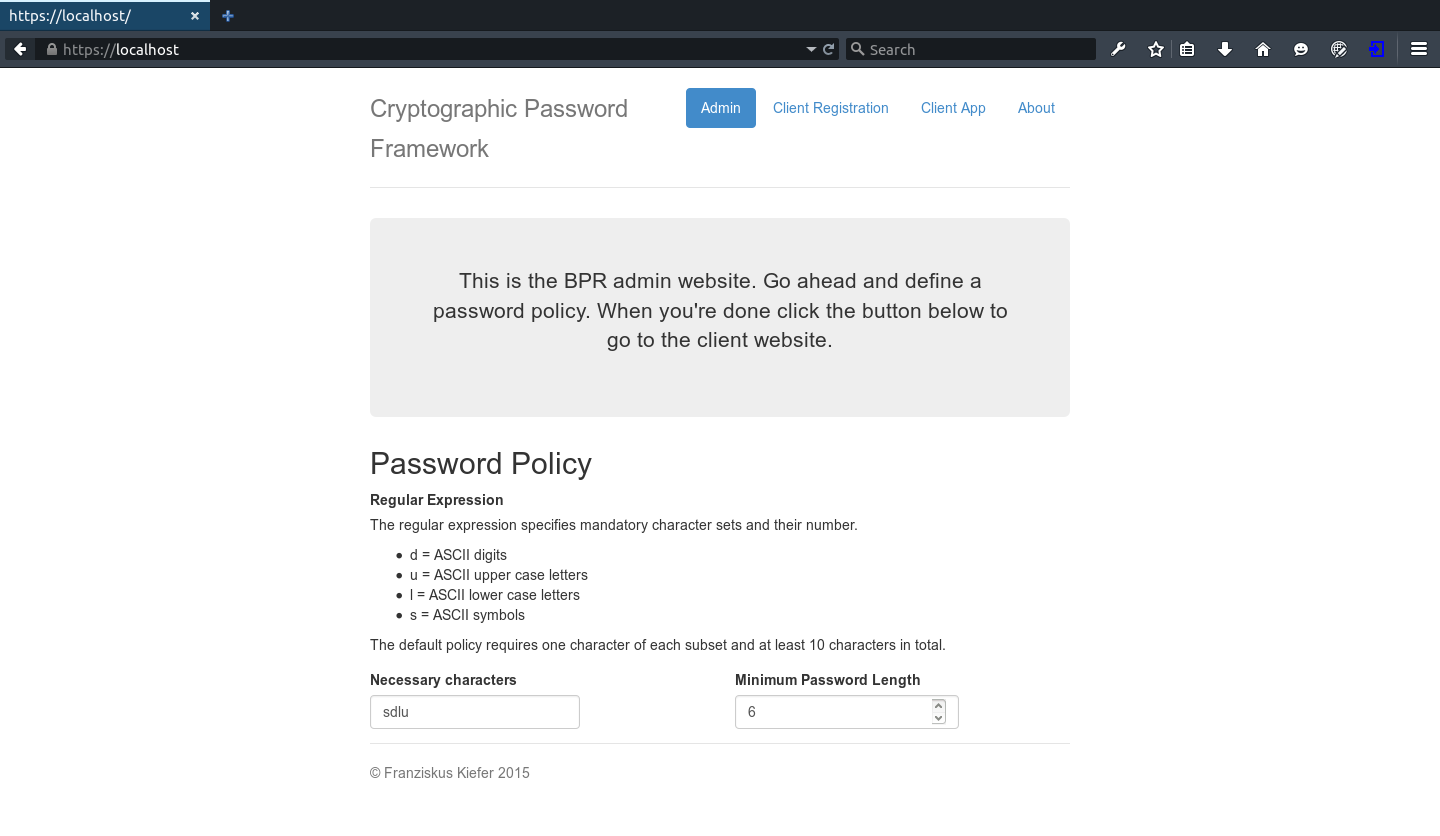
\includegraphics[width=0.98\textwidth]{Figs/demo-admin.png}
\caption{Demo --- Admin interface}\label{fig:demo-admin}
\end{figure}

\paragraph{Client Interface}
Selecting the \emph{Client Registration} link presents the user with a simple website asking the user to register a new user and password.
To this end the user has to click the registration/login button in the browser toolbar to open the registration form.
This button is only active for websites that support the \ac{BPR} registration process and provides the user with a trusted path to a trusted registration form.
Note that it is important that the registration form is trusted and \emph{not} provided by the server as the server is not trusted with secure handling of the client password.
After clicking ``Register Now'' the extension performs the \ac{BPR} protocol from Section \ref{sec:bpr} with the server.
The JavaScript implementation makes use of cryptographic libraries\footnote{\url{http://www-cs-students.stanford.edu/~tjw/jsbn/},\\\hspace*{1.5em} \url{https://github.com/bitwiseshiftleft/sjcl}}), while the server uses the Charm library by \citet{charm13}.

\begin{figure}[tbph]
\centering
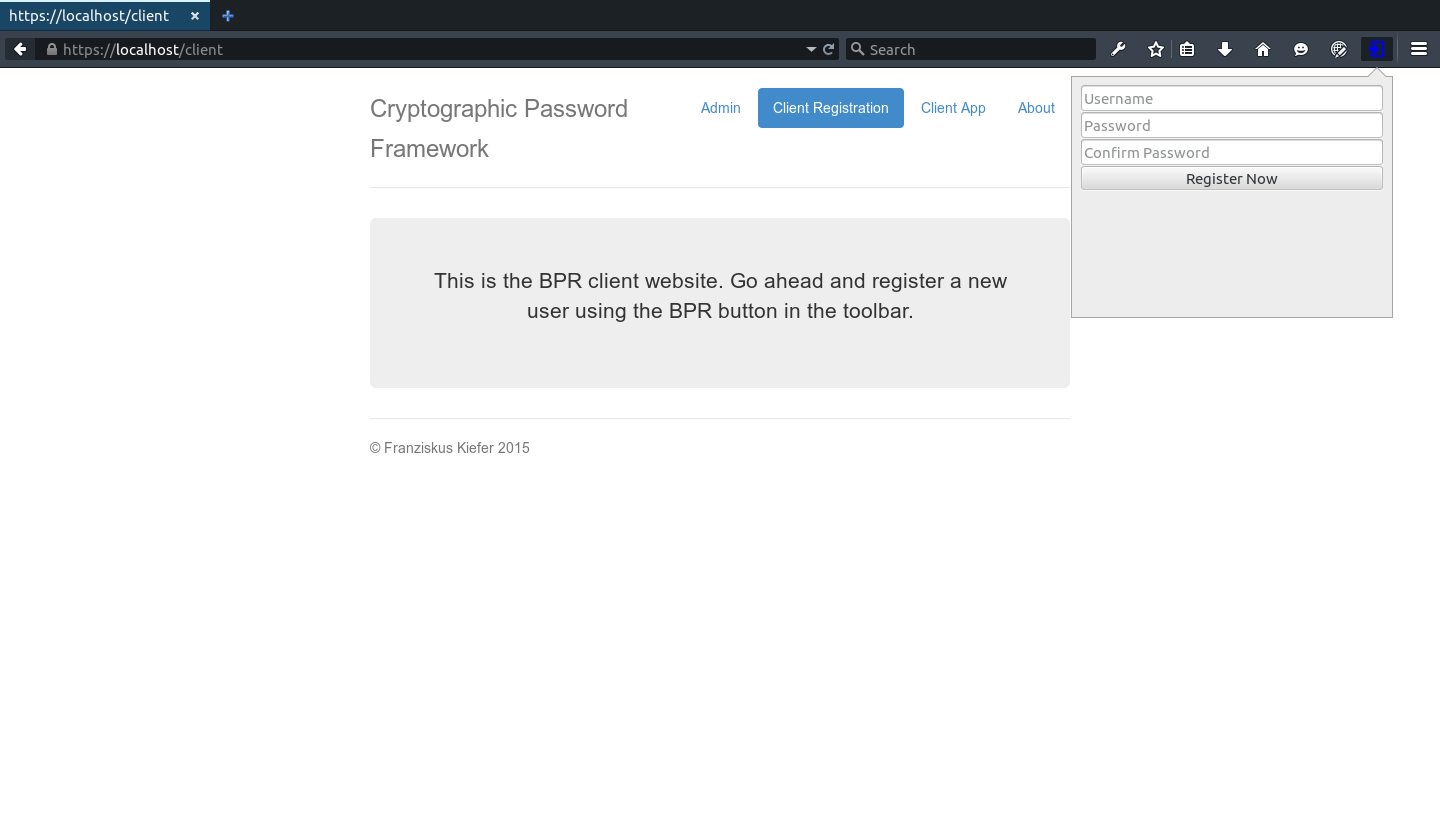
\includegraphics[width=0.98\textwidth]{Figs/demo-register-popup.png}
\caption{Demo --- Client Registration interface}\label{fig:demo-register}
\end{figure}

\subsection{Login}
Clicking on the ``Client App'' link provides the user with a simple website asking the user to log into the application using the registration/login button in the browser toolbar.
Similar to the registration process, the user is presented with a trusted login form.
After entering user name and password, and clicking ``Login'', the extension performs the tSoke protocol with the server.
As discussed before, tSoke is a \ac{VPAKE} protocol that additionally uses a tag to make it usable in the \ac{PACCE} setting.
Thereby, client and server perform a \ac{PACCE} protocol, which hands the session over to the client application when done.

\begin{figure}[tbph]
\centering
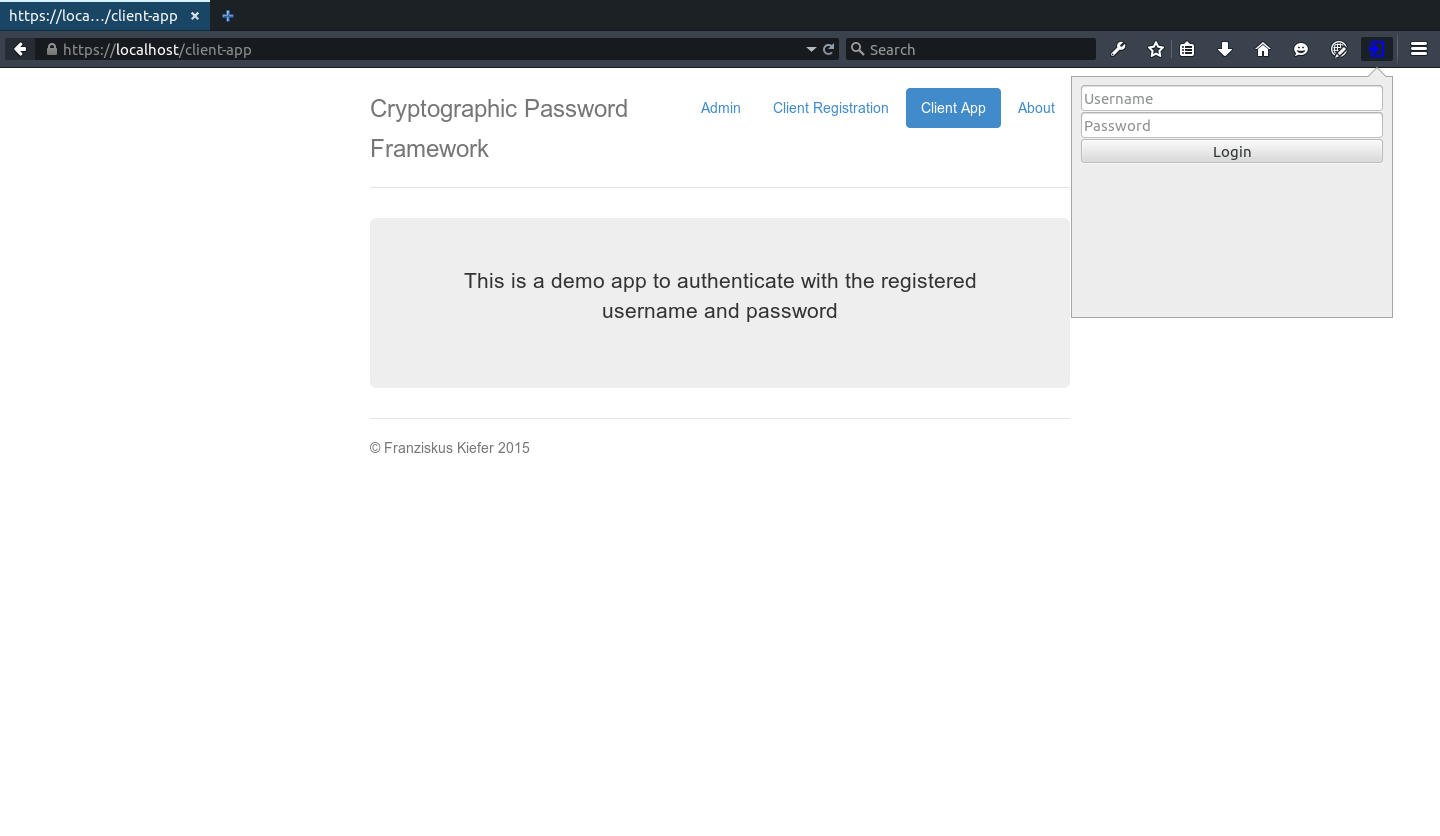
\includegraphics[width=0.98\textwidth]{Figs/demo-login-popup.png}
\caption{Demo --- Client Login interface}\label{fig:demo-login}
\end{figure}

\subsection{Demo Application}
The client demo application, a simple to-do application, is depicted in Figure \ref{fig:demo-app}.
It is an independent component and embedded in the framework website as an iframe.
It uses NodeJS\footnote{\url{https://nodejs.org/}} as RESTful\footnote{\url{https://en.wikipedia.org/wiki/Representational_state_transfer}} server, MongoDB\footnote{\url{https://www.mongodb.org/}} for storage, and jade\footnote{\url{http://jade-lang.com/}} as template engine.

\begin{figure}[tbph]
\centering
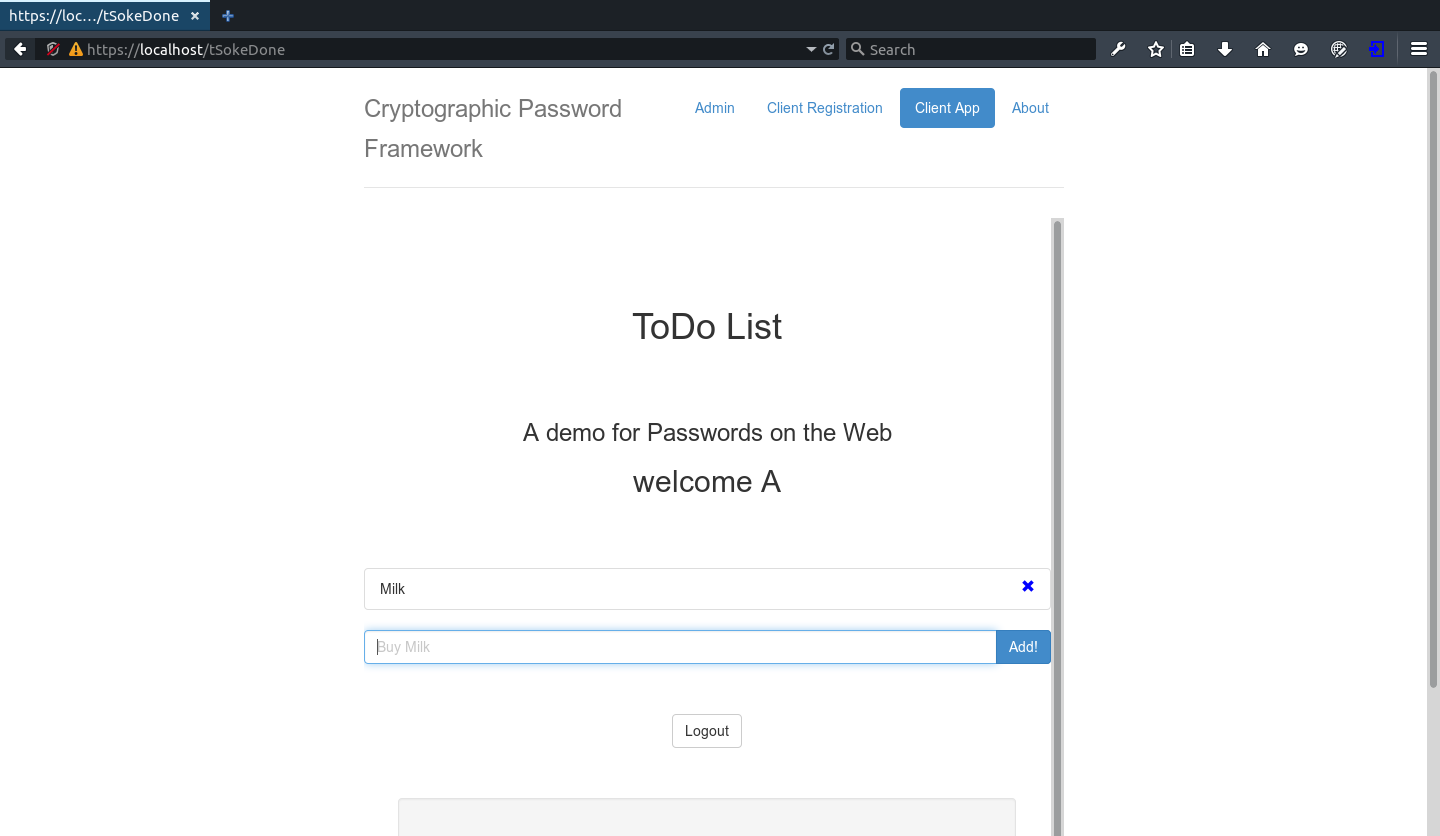
\includegraphics[width=0.98\textwidth]{Figs/demo-app.png}
\caption{Demo --- Client Application interface}\label{fig:demo-app}
\end{figure}


% \section{Extending the Framework -- Oblivious VPAKE}
% \mynote{OVPAKE for password trials \cite{Kiefer2012,Kiefer13a} (not implemented)}

\section{Conclusion} \label{sec:vpake-conclusion}
This chapter proposed a password registration and authentication framework for the single server setting, gave efficient instantiation and a demo application to show its use.
Using \ac{ZKPPC} from as basis, Section \ref{sec:bpr} proposed an efficient \acl{BPR} protocol with security model.
An alternative approach to the problem of \ac{BPR} is proposed in Section \ref{sec:spc-bpr}, using a set theoretic approach.
Comparison of the two proposed \ac{BPR} protocols show that the set-based approach is significantly faster due to the use of symmetric primitives, while requiring a different security model.
The second step in the framework, password-based authentication, is solve by a new \ac{VPAKE} protocol.
Implementation and demonstrator showed practicability of the proposed approach.

\chapter{Password Authentication Framework for the Two-Server Setting} \label{ch:2pake}

While \ac{PAKE} and \ac{VPAKE} solve one of the most pressing problems in user authentication they are still vulnerable to offline dictionary attacks once the server is compromised.
To alleviate the impact of password leaks on the server threshold \ac{PAKE} has been proposed.
However, research in this area is rather limited compared to the single-server case.
This chapter proposes a framework for the two-server setting, similar to the framework from Chapter \ref{ch:vpake}, which uses \ac{2PAKE} for user authentication and a \ac{2BPR} protocol for password share registration.
We further propose a new security model for two \ac{2PAKE} protocols in the \ac{UC} model.

This chapter is based on work in \cite{KieferM14b,KieferM15b,KieferM15c}.

\paragraph{Introduction}

Considering that ``password-cracking tools'' such as Hashcat \cite{hashcat} and John the Ripper \cite{JohnTheRipper} are very efficient, it is reasonable to assume that leaking password hashes is more or less equivalent to leaking passwords \cite{NarayananS05a,WeirAMG09,DellAmicoMR10,Bonneau12}.
The notion of threshold and two-server password authenticated key-exchange \cite{FordK00,MacKenzieSJ02} has been proposed where the password is not stored on a single server but split between a number of servers such that leakage of a password database on a non-qualified subset does not reveal the password.
The two-server setting is regarded as more practical (in comparison to a more general threshold setting) given that if one server is compromised a notification to change the password can be sent out to the clients.
\ac{2PAKE} protocols \cite{BrainardJKS03,SzydloK05,Katz2012a} split the client's password $\pwd$ into two shares $\share_1$ and $\share_2$ such that each share is stored on a distinct server.
During the authentication phase both servers collaborate in order to authenticate the client.
Yet, no server alone is supposed to learn the plain password.
A second, more recent development in two-server (and threshold) password protocols is \ac{PPSS} \cite{Bagherzandi2011,Camenisch2012,JareckiKK14} where a client stores shares of a (high-entropy) secret key on a number of servers and uses a (low-entropy) password to authenticate the retrieval process.

Registering password shares for \ac{2PAKE}/\ac{PPSS} protocols however makes it impossible for the servers to verify their password policies upon registration unless the password is transferred to each of them in plain. 
This however, would imply that the client trusts both servers to securely handle the password, which contradicts the purpose and trust relationships of multi-server protocols.
The use of two-server password protocols in a remote authentication setting, therefore, requires a suitable password registration procedure in which none of the servers would receive information enabling it (or an attacker in control of the server) to deliberately or inadvertently recover the client's password.
This registration procedure must further allow for policy compliance checks to be performed by the servers since secret sharing does not protect against weak passwords.
A trivial approach of sending $\share_1$ and $\share_2$ to the corresponding servers over secure channels is not helpful here since it is not clear how the two servers can perform the required compliance check.

The concept of blind password registration for two-server password protocols proposed as first step in this chapter shows how to realise secure registration of password shares in a way that protects against at most one malicious server (if both servers are malicious, the attacker obviously gets the password), yet allows both servers to check password compliance against their mutual password policy.
\ac{2BPR} is not vulnerable to offline dictionary attacks as long as one server remains honest.
This is in contrast to the single-server setting where an attacker is always able to perform offline dictionary attacks on password verifiers after compromising a server. 

The second step in the framework can either be a \ac{2PAKE} or a two-server \ac{PPSS} protocol.
We show how to use password shares set up with the \ac{2BPR} protocol to authenticate the client.
Further, we propose a new framework for \ac{2PAKE} protocols that leads to a new security model for \ac{2PAKE} protocols in the \ac{UC} model.

%password BPR protocol
% Our main contribution is the 2BPR security model and the corresponding protocol for secure registration of 2PAKE/2PASS passwords. We show how secure distribution of password shares can be combined with an appropriate policy-compliance proof for the chosen password in a way that does not reveal the password and can still be verified by both servers.
% Our 2BPR protocol can be used to enforce policies over the alphabet of all 94 printable ASCII characters, including typical requirements on password length and character types.

% \paragraph{Two-Server Password Authenticated Key Exchange}

% \ac{PAKE} protocols have been extensively researched over the last twenty years.
% They allow two protocol participants, holding a low-entropy secret (password) each, to negotiate an authenticated session key.
% Several security models have been developed including the well-known game-based notion from Bellare, Pointcheval and Rogaway \cite{Bellare2000,Abdalla2005a} and a notion in the universal composability (UC) framework \cite{Canetti2005}.
% While PAKE protocols can be executed between two humans holding the same password, they are usually considered in a client, server scenario where the client registers with a server that then stores the password and uses it in subsequent sessions to authenticate the client.
% This approach however leads to an intrinsic weakness regarding server compromise.
% As soon as a server, storing client passwords is compromised the attacker learns the passwords.
% This allows the attacker to log into the client's account on the server and most likely also on others if the client re-used the password across multiple servers.
% Mechanisms have been proposed to solve the problem of server compromise.
% In particular verifier-based PAKE \cite{Gentry2006,rfc2945,BenhamoudaP13}, also known as augmented PAKE \cite{BellovinM93}, considers an asymmetric setting in which the server uses a function of the password (verifier) to verify a client holding the corresponding password.
% However, as long as only one server is used, PAKE protocols are prone to offline dictionary attacks on the server side, i.e. server attacks still leak password verifiers that allow to recover the password, which is rather efficiently with current methods \cite{hashcat,JohnTheRipper}.

% \ac{2PAKE} protocols solve the problem of offline dictionary attacks in the case of server compromise by splitting the password in two parts such that a malicious or compromised server can only recover a password share that does not allow to recover the password.
% % In contrast to \ac{PAKE} protocols \ac{2PAKE} protocols are less well studied.
% % 2PAKE can be seen as a special case for $t=n=2$ of threshold PAKE where $t$ out of $n$ servers, participating in the protocol and holding a password share, must be honest.
% \citet{RaimondoG03} and \citet{MacKenzieSJ02} were among the firsts to propose t-out-of-n password authenticated key exchange protocols.
% The former is not suitable for \ac{2PAKE} as it needs $t<n/3$ while the latter requires a PKI in addition to the password.
% The first real two-server PAKE protocol is due to Brainard and Jules \cite{Brainard_Juels_2003}, which was proven secure by Szydlo and Kaliski \cite{SzydloK05} in a modified version.
% The first two server PAKE with thorough security model based on the classical game-based BPR model is due to Katz, MacKenzie,  Taban and Gligor \cite{KatzMTB05}, which was recently generalised to a two-server PAKE framework by Kiefer and Manulis \cite{KieferM14a}.
% Threshold and two-server password authenticated key exchange is closely related to password authenticated secret sharing (PASS).
% Password authenticated secret sharing was first proposed as password protected secret sharing by Bagherzandi, Jarecki, Saxena and Lu in 2011 \cite{Bagherzandi2011} and gained a lot of attention since then \cite{Camenisch_Lysyanskaya_Neven_2012,JareckiKK14,CamenishEN15}.
% As shown in \cite{JareckiKK14} PASS can also be used to implement efficient threshold PAKE protocols.
% While using the universally composability framework to prove security of the PASS primitive, none of these papers give a threshold or two-server PAKE protocol secure in UC.
%
% In this work we propose the first notion of UC security for two-server PAKE protocols and give an efficient protocol in the standard model with common reference string and static corruptions.
% To this end we leverage recent advancements of smooth projective hashing in the two-server setting from \cite{KieferM14a} and in efficiency from \cite{Benhamouda2013}.

\paragraph{Outline}
This chapter consists of six sections.
The first section describes modelling of passwords, policies and password shares for the two-server setting.
Section \ref{sec:2pake-registration} proposes a \acl{BPR} for the two-server setting, closely related to the approach in Chapter \ref{ch:vpake} Section \ref{sec:bpr}.
This concludes the registration step of the framework.
For the authentication step Section \ref{sec:twoserverpake} proposes a \ac{2PAKE} framework using \acp{D-SPHF} that are introduced in Section \ref{sec:dsphf-2pake}.
To strengthen security guarantees of \ac{2PAKE} protocols we propose a security definition of \ac{2PAKE} in the \ac{UC} framework in Section \ref{sec:uc2pake}.

\section{Modeling Passwords and Policies}

\subsection{Passwords}
We adopt the reversible, structure-preserving encoding scheme from \cite{KieferM14c} that (uniquely) maps strings of printable ASCII characters to integers.
We use \pwd for the ASCII password string, $c_i=\pwd[i]$ for the $i$-th ASCII character in \pwd, and integer $\pi$ for the encoded password string.
The encoding proceeds as follows: $\pi\gets\pwdint(\pwd)=\sum_{i=0}^{n-1}b^{i} (\ASCII(c_i)-32)$ for the password string \pwd and $\pi_i\gets\chrint(c_i)$ $=\ASCII(c_i)-32$ for the $i$-th \emph{unshifted} ASCII character in \pwd.
Note that $n$ denotes the length of \pwd and $b\in\NN$ is used as shift base.
(We refer to \cite{KieferM14c} for a discussion on the shift base $b$. Note, however, that shift base related attacks on the password verifier from \cite{KieferM14c} are not possible in our two-server setting.) The \ASCII function returns the decimal ASCII code of a character.
In our protocol we will consider the case where password strings \pwd are chosen uniformly at random or according to some distribution with min-entropy $\beta$ from dictionary \cD.

\begin{remark}\label{rem:passwords}
While password distribution is important for the security of a password registration protocol in the verifier-based PAKE setting \cite{KieferM14c}, the password distribution plays a different role in the two-server setting.
Since the server stores only a password share instead of a password verifier, offline dictionary attacks from an attacker controlling only one of the two servers are impossible.
% (Note that this does not mean online dictionary attacks on a registered password are not possible. However, this is out of scope of the security model for a password registration protocol.)
The notion for 2BPR proposed in this work is therefore independent of the password, chosen by the client.
Note however that the password strength still continues to play a role in the usage of 2PAKE/2PASS protocols, where it influences the probability of successful online dictionary attacks.
% That said, one has to be careful not to assume that the client's password choice is not important for the overall security of the system.
% However, this only comes into play in subsequent use of the password but \emph{not} in the setup.
\end{remark}

\subsection{Password Sharing}
We focus on the additive password sharing of client passwords, i.e. $\pi=\share_0+\share_1 \mod q$ over a prime-order group $G_q$.
Such sharing has been used in various two-server PAKE protocols, including  \cite{Katz2005,Yang_Deng_Bao_2006,Jin_Wong_Xu_2007,Kiefer14}.
To be used in combination with two-server password authenticated secret sharing protocols such as \cite{CamenischLN2012} one can define the password as $g^\pi$ and thus create a multiplicative sharing $g^\pi=g^{\share_0}g^{\share_1}$.
Password shares are created as $\share_0\rin\ZZ_q$ and $\share_1=\pi-\share_0 \mod q$.
We remark that other sharing options such as xor \cite{Brainard2003,SzydloK05} have been used in literature but these are not supported by our protocol.


\subsection{Password Policies}
We represent password policies using an approach based on \cite{KieferM14c}, i.e. a password policy $f=(R,\pmin)$ consists of a simplified regular expression $R$ that defines ASCII subsets that must be present in the chosen password string and the minimum length \pmin of the password string.
Note that we do not require a maximum password length \pmax.
$R$ is defined over the \emph{four} ASCII subsets $\Sigma=\{d,u,l,s\}$ with digits $d$, upper case letters $u$, lower case letters $l$ and symbols $s$, and gives the minimum frequency of a character from the subset that is necessary to fulfil the policy; for instance, $R=ulld$ means that the password string must contain at least one upper case letter, two lower case letters and one digit.
In the two-server password setting each of the two servers may have its own policy, i.e. $f_0$ and $f_1$.
The registered passwords must comply with their \emph{mutual policy} defined as $f=f_0\cap f_1=(\max(R_0,R_1),\max(\pmin_0,\pmin_1))$, where $\max(R_0,R_1)$ is the regular expression with the maximum number of characters from each of the subsets $u,l,d,s$ from the two expressions $R_0$ and $R_1$.
%we define the intersection of two policies $f_0$ and $f_1$ that passwords registered through our 2BPR protocol will need to fulfil, namely
A mutual policy is fulfilled, i.e. $f(\pwd)=\true$, iff $f_0(\pwd)=\true$ and $f_1(\pwd)=\true$, and not fulfilled, i.e. $f(\pwd)=\false$, iff $f_0(\pwd)=\false$ or $f_1(\pwd)=\false$.
We mainly operate on the integer representation $\pi$ of a password \pwd throughout this paper and sometimes write $f(\pi)$, which means $f(\pwd)$ for $\pi\gets\pwdint(\pwd)$.
Further note that a character $c_i\in\pwd$ is called \emph{significant} if it is necessary to fulfil a policy expression $R$ and we say the corresponding set $R_j\in R$ is the according \emph{significant set}.


%********************************** %2PAKE Registration  **************************************
% \mynote{2BPR ???(ePrint/ESORICS'15) \cite{KieferM15c}}
\section{Two-Server Blind Password Registration} \label{sec:2pake-registration}
\ac{2BPR} allows a client to register password shares with two servers for later use in \ac{2PAKE}/\ac{PPSS} protocols and prove that the shares can be combined to a password that complies with the mutual password policy of both servers, without disclosing the password.
% The password shares can later be used in two-server PAKE protocols or two-server password protected secret sharing (cf. Section \ref{sec:application}).
A \ac{2BPR} protocol is executed between client $\Client$ and two servers $\Server_0$ and $\Server_1$ with password policies $f_0$ and $f_1$ respectively.
\Client interacts with $\Server_0$ and $\Server_1$ in order to distribute shares of a freshly chosen password string \pwd and prove its compliance with the mutual policy, \ie $f_0(\pwd)=\true$ and $f_1(\pwd)=\true$.
A \ac{2BPR} protocol between an honest client $\Client$ and two honest servers $\Server_0$ and $\Server_1$ is correct if $\Server_0$ and $\Server_1$ accept their password shares if the client is able to prove the following statement for $f=f_0\cap f_1$:
\begin{align}
  (\pwd,\share_0,\share_1):~ \pwdint(\pwd)=\share_0+\share_1 ~ \wedge ~ f(\pwd)=\true.
  \label{eq:zkppc-pok}
\end{align}
Note that the \ac{2BPR} protocol can be used to register new clients or to register new passwords for existing clients. The following definition formally captures the functionality of \ac{2BPR} protocols.

\begin{definition}[Two-Server Blind Password Registration]\label{def:2bpr}
A \ac{2BPR} protocol is executed between a client $\Client$ and two servers $\Server_0$ and $\Server_{1}$, holding a password policy $f_b$ each, such that the servers, when honest, eventually accept password shares $\share_b$ of a policy compliant, client chosen password \pwd iff $f(\pwd)=\true$ for $f=f_0\cap f_1$, $\pwdint(\pwd)=\share_b+\share_{1-b}$ and $b\in\{0,1\}$.
\eod
\end{definition}

\noindent
Definition~\ref{def:2bpr} requires that password shares $\share_0$ and $\share_1$ can be combined to the policy-compliant integer password $\pi$. The corresponding verification must therefore be part of the \ac{2BPR} protocol. 
Otherwise, the client could register password shares $\share_0$ and $\share_1$ that can both be combined to a policy compliant password in the respective proofs with the servers, but combining $\share_0$ and $\share_1$ might result in a password that is \emph{not} policy compliant, \ie $f(\share_0+\share')=\true$ and $f(\share_1+\share'')=\true$ but $f(\pi)\not=\true$.
This further ensures that servers hold valid password shares, which is crucial for the security of \ac{2PAKE}/\ac{PPSS} protocols that should be executed later with these password shares.
We assume that the servers distributed their policy to the client before the protocol starts.
We further assume that the servers communicate with each other in order to confirm correctness of the password shares.
This requirement can be relaxed by requiring the client to forward messages (authenticated and confidential) between the two servers.
For simplicity however we assume direct communication between the two servers in our model.


\subsection{Model}\label{sec:securitymodel}
Security of \ac{2BPR} protocols, given according to Eq. (\ref{eq:zkppc-pok}), has to guarantee that the client knows the sum $\pwdint(\pwd)$ of the password shares $\share_0$ and $\share_1$, and that \pwd fulfils both password policies $f_0$ and $f_1$ in case both servers accept the registration.
This model is related to the \ac{BPR} model from Chapter \ref{ch:vpake} Section \ref{sec:bpr} but requires handling of two servers and server corruption.
We translate Eq. (\ref{eq:zkppc-pok}) into a game-based security model that captures the relation using two different security definitions.
The first notion, like in \ac{BPR}, can be directly converted from Eq. (\ref{eq:zkppc-pok}) and captures \acl{PC} of the password.
In particular, if both servers are honest while accepting their password shares in the \ac{2BPR} protocol, the combination $\pi$ of the shares represents a password compliant with the mutual password policy $f=f_0\cap f_1$, \ie $f(\share_b+\share_{1-b})=\true$.
The second notion relates to the fact that servers should not learn anything about the password and therefore called \ac{PB}, in contrast to \ac{BPR}, where the server is always able to perform offline dictionary attacks on the password verifier.
\ac{PB} requires that a malicious server $\Server_b$ must not be able to learn anything else from the \ac{2BPR} execution about the client's password than the fact that it is policy compliant.

We observe that the blindness property has to hold for all possible password policies and all compliant passwords. It should not be possible to mount an offline dictionary attack after observing \ac{2BPR} protocol executions or while gaining access to and controlling at most one of the two servers.

\paragraph{Setup and Participants}
Protocol participants $\Client,\Server_0,\Server_1$ with $\Client$ from the universe of clients and $\Server_1,\Server_2$ from the universe of servers have common inputs, necessary for the execution of the protocol. %, such as group parameters, the common reference string, the server's public keys and according policies $f_1,f_2$.
Instances of protocol participants \Client or \Server are denoted $\Client_i$, $\Server_{0,i}$ or $\Server_{1,i}$.
Protocol participants without specified role are denoted by $P$, and $\Server_b$ and $\Server_{1-b}$ for unspecified servers.
A client can only register one password with one server pair, but can register passwords at an arbitrary number of server pairs.
Client $\Client$ and servers $\Server_b$ are unique and used as identifier on the server, \ie as \emph{username} to store alongside the password share on $\Server_{1-b}$.
We say a client registers a client, server pair at a server, \ie a client $\Client$ registers a password share for $(\Client, \Server_{1-b})$ at a server $\Server_b$ and a password share for $(\Client,\Server_{b})$ at server $\Server_{1-b}$.
Further, a server only allows a single registration from a client, server pair such that any attempt to register a password with a server that already stores a password share for this client, server pair overwrites existing entries, \ie resets the password.
An entry $(\Client,\Server_{1-b},\share_b)$ is only stored on server $\Server_b$ if the \ac{2BPR} protocol is successful.

\paragraph{Oracles}
To interact with protocol participants, \ac{PPT} adversary \cA has access to \Setup, \Send, \Execute and \Corrupt oracles.
% We say a message $m$ is \emph{rogue} if it is either generated by the adversary or by an oracle and then modified by the adversary or by an oracle but for a different session.

\begin{itemize}
  \item $\Setup(\Client,\Server_0,\Server_1, \pwd')$ creates new instances of all participants and stores identifiers of the other parties to each participant.
        To this end the client receives the server policies $f_0\cap f_1=f$ and either chooses a new policy compliant password $\pwd\in\cD_f$ if $\pwd'=\bot$ or uses $\pwd=\pwd'$.
%         This oracle models the initial registration request by the client and returns the first server messages $m_0$ and $m_1$ with $m_b$ honestly generated if $m'_b=\bot$ or $m_b\gets m'_b$ otherwise for $b\in\bits$.

  \item $\Execute(\Client,\Server_0,\Server_1)$ models a passive attack and executes a \ac{2BPR} protocol between new instances of $\Client$, $\Server_0$ and $\Server_1$. %, initiated with \Setup.
%         If there exists an entry $(C,\Server_1,\share_0)$ at $\Server_0$ or $(C,\Server_2,\share_1)$ at $\Server_2$, the oracle aborts.
        It returns the protocol transcript and the internal state of all corrupted parties.
%         Note that communication between the protocol is confidential such that the adversary only learns ciphertexts unless he corrupted one of the participants.

  \item $\Send_\Client(\Client,\Server_{b,j},m)$ sends message $m$, allegedly from client $\Client$, to server instance $\Server_{b,j}$ for $b\in\{0,1\}$.
        If $\Server_{b,j}$ does not exist, the oracle aborts. %or there exists an entry $(C,\Server_2,\share_1)$ at $\Server_1$ or $(C,\Server_1,\share_2)$ at $\Server_2$,
        Note that any instance $\Server_{b,j}$ was thus set up with \Setup and therefore has an according partner instance $\Server_{1-b,j}$.
        If all participants exist, the oracle returns the server's answer $m'$ if there exists any.
        Necessary inter server communication is performed in $\Send_\Client$ queries.
        If $m=\bot$, server $\Server_{b,j}$ returns its first protocol message if it starts the protocol.
        % if both servers are honest.
%         If $\Server_{1-b}$ is corrupt, the oracle additionally returns message $m'_\Server$ from $\Server_{b,i}$ to $\Server_{1-b,i}$ if such a message is sent in the protocol.
%         This oracle can model a passive attack if the message $m$ is not rogue, or an active attack if $m$ is rogue.

  \item $\Send_\Server(\Server_{b},\Client_{j},m)$ sends message $m$, allegedly from server $\Server_{b}$ for $b\in\{0,1\}$, to client instance $\Client_{j}$.
        If $\Client_j$ does not exist, the oracle aborts.
        Note that any instance $\Client_j$ was set up with \Setup and therefore has an according partner instance $\Server_{1-b,i}$.
        If all participants exist, the oracle returns the client's answer $m'$ if there exists any.
        If $m=\bot$, server $\Server_{b}$ returns its first message if he starts the protocol.
%         This oracle can model a passive attack if the message $m$ is not rogue, or an active attack if $m$ is rogue.

  \item $\Send_{\Server\Server}(\Server_{b},\Server_{1-b,j},m)$ sends message $m$, from server $\Server_{b}$ for $b\in\{0,1\}$, to server instance $\Server_{1-b,j}$.
        If $\Server_{1-b,j}$ does not exist, the oracle aborts.
        Note that any $\Server_{1-b,j}$ was set up with \Setup.
        If all participants exist, the oracle returns the server's answer $m'$ if there exists any.

  \item $\Corrupt(\Server_{b})$ allows the adversary to corrupt a server $\Server_b$ and retrieve its internal state, \ie stored messages and randomness, and the list of stored password shares $(\Client, \Server_{1-b}, \share_b)$. % if no instance of $\Server_b$ is active.
      $\Server_b$ is marked \emph{corrupted}.
%       Otherwise the oracle aborts.
\end{itemize}

\noindent
Note that we allow the adversary to register passwords with servers such that we do not require the existence of a client instance $\Client_i$ after a successful registration (client identities $\Client$ are unique but not secret and can therefore be used by the adversary).

\paragraph{Policy Compliance}
\ac{PC} is the first natural security property of \ac{2BPR} protocols, requiring that a password set up with a \ac{2BPR} protocol by a client is compliant with the policy of the two servers $f(\pwd)=\true$.
The attacker here plays the role of the client that tries to register a password \pwd that is \emph{not} policy compliant on two honest servers.

% XXX: \fk{We should think about if it is sensible to allow password reset. In real the world the server would require the client to login before changing the password (authentication is done via e-mail usually if password is not known anymore). Therefore the adversary should be allowed to change passwords for triple $(C,\Server_0,\Server_1)$ that executed the protocol successfully already.}

\begin{definition}[Policy Compliance]\label{def:pc}
\acl{PC} of a \ac{2BPR} protocol holds if for every \ac{PPT} adversary $\cA$ with access to $\Setup$ and $\Send_\Client$ oracles the probability that two server instances $\Server_{b,i}$ and $\Server_{1-b,j}$ exist after $\cA$ stopped that accepted $(\Client,\Server_{1-b},\share_b)$, $(\Client,\Server_{b},\share_{1-b})$ respectively, with $f(\share_b+\share_{1-b})=\false$ is negligible.
\eod
\end{definition}

\paragraph{Password Blindness}
The second security property requires that every password, chosen and set up by an honest client must remain hidden from an adversary even if he corrupts one of the two used servers, gets its internal state and controls its actions.
We model this with a distinguishing experiment where the attacker, after interacting with the oracles, outputs a challenge comprising two passwords $\pwd_0$ and $\pwd_1$, two clients $\Client_0$ and $\Client_1$, and a pair of servers $\Server_0$ and $\Server_1$.
After randomly assigning the two passwords to the two clients, the adversary interacts with the oracles again and has to decide which client uses which password, \ie guess the random bit $b$.
The notion is formalised in the following definition.

\begin{definition}[Password Blindness]\label{def:zk}
The \acl{PB} property of a \ac{2BPR} protocol $\Pi$ holds if for every \ac{PPT} adversary $\cA$ there exists a negligible function $\varepsilon(\cdot)$ such that
% for $t$ passwords set-up for $(\Client,\Server_0,\Server_1)$
\[ \Adv_{\Pi, \cA}^{\mathrm{PB}}=\left|\Pr[\Exp_{\Pi, \cA}^{\mathrm{PB}}=1]-\frac{1}{2}\right|\leq\varepsilon(\secpar). \]

\noindent
$\Exp_{\Pi, \cA}^{\mathrm{PB}}:$ \\
\hspace*{2em} $(\Client_0, \Client_1, \Server_0,\Server_1,\pwd_0,\pwd_1)\gets\cA_1^{\Setup(\cdot),\Send_\Server(\cdot),\Send_{\Server\Server}(\cdot), \Execute(\cdot),\Corrupt(\cdot)}$ $(\secpar,\cD,\{\Client\},\{\Server\})$ \\
\hspace*{2em} check $\pwd_0,\pwd_1\in\cD_{f_0\cap f_1}$, $|\pwd_0|=|\pwd_1|$, $\Client_0,\Client_1\in\{\Client\}$ and $\Server_0,\Server_1\in\{\Server\}$\\
\hspace*{2em} $ b'\gets\cA^{\Setup'(\cdot),\Send_\Server(\cdot),\Send_{\Server\Server}(\cdot), \Execute(\cdot),\Corrupt(\cdot)}(\secpar,\cD,\{\Client\},\{\Server\})$\\
\hspace*{2em} if $\Server_0$ or $\Server_1$ is not corrupted, return $b=b'$; otherwise return $0$ \\

\noindent
$\Setup'$ (in contrast to \Setup) uses $\pwd_b$ for client $\Client_0$ and $\pwd_{1-b}$ for $\Client_1$ with $b\rin\bits$ instead of choosing a random password or using the provided one.
\eod
\end{definition}


% ==================================================================================
% Two-Server BPR Protocol
% ==================================================================================

\subsection{An Efficient Two-Server BPR Protocol}\label{sec:framework}
Before describing technical details, we give a high-level description of our \ac{2BPR} protocol.
We assume that client $\Client$ selected two servers $\Server_0$ and $\Server_1$ to register with, and server authenticated channels between each of the two servers and the client as well as between the two servers have been established.
Note that the connection between the two servers is necessary in order to verify the correctness of the password shares.
% If a direct connection between the two servers is not possibleA weaker security notion where correctness is not necessary is possible.
Server authenticated and confidential channels between each server and the client is a rather weak assumption that can be implemented with a \ac{TLS} channel \cite{rfc5246,JagerKSS12,KrawczykPW13}.
This essentially prevents the attacker from querying the $\Send_\Server$ or $\Send_{\Server\Server}$ oracle without prior corruption of the according server and further provides an attacker only with encrypted transcripts unless he performs active attacks or corrupts a participating server.
% We describe the protocols internal functionality in the following paragraph without explicit description of the encrypted channel.
The protocol further relies on a common setup, given a \ac{CRS}.
The \ac{CRS} contains all necessary parameters, \ie $\crs=(g, h, p)$ with generators $g$ and $h$ for group of prime-order $p$ where $\log_g(h)$ is not known.
At the beginning of the registration phase the client commits to the integer representation $\pi$ of the chosen password string \pwd and sends this commitment together with a password share $\share_b$ to the corresponding server $\Server_b$, $b\in\bits$, along with auxiliary information that is needed to perform the \ac{PC} proof.
For the latter, the client needs to prove the knowledge of $\pi$ in the commitment such that $\pi = \share_0 + \share_1$ and that it fulfils both policies $f_1$ and $f_2$.
Thus, servers $\Server_0$ and $\Server_1$ eventually register the new client, accept and store the client's password share, iff each $\Server_b$ holds $\share_b$ such that $\share_0+\share_1=\pi$ for $\pi\gets\pwdint(\pwd)$ and $f(\pwd)=\true$ for $f=f_0\cap f_1$.

The general protocol is similar to the \ac{BPR} protocol proposed in Chapter \ref{ch:vpake} Section \ref{sec:bpr} for the single server setting.
While \acl{PoM} and \ac{PoS} are essentially the same, a \ac{PoC} replaces the \ac{PoE} from \ac{BPR} to prove correctness of shares.
We further require zero-knowledge proofs that are secure against malicious verifiers (servers) since the attacker is allowed to corrupt one server in the protocol, \ie we do not assume semi-honest servers.

\subsubsection{Protocol Overview}
% \begin{figure}[!b]
% \centering
% \footnotesize
% \scalebox{0.8}{\begin{tikzpicture}%[framed]
% \draw[] (-3.5,1) rectangle (12.3,-13);
% \draw ($(-3,.7)!0.55!(12,.7)$) node[draw] {\textit{I -- Client Preparation}};
%
% \node[party,align=center] (client) at (.5,0) {\uline{$\Client~ (\Server_0,\Server_{1}, f_0, f_1, \pwd, \crs)$}};
%
% \node[state, align=left] at (0,-.5) [stateS, align=left]{Encode $\pi\gets\pwdint(\pwd)$;};
% \node[state, align=left] at (0,-1.2) [stateS, align=left]{Compute password shares: $\share_{0}\rin\ZZ_p$,\\ \hspace*{1em} $\share_{1}=\pi-\share_{0}$};
%
% \node[state, align=left] at (0,-2.3) [stateS, align=left]{Commit to shares: \\\hspace*{1em} $\fC_0=g^{\share_{0}}h^{r_{0}}$, $\fC_{1}=g^{\share_{1}}h^{r_{1}}$\\ \hspace*{1em} $\fD_0=\fC_0g^{\share_{1}}$, $\fD_{1}=\fC_{1}g^{\share_{0}}$};
%
% % PHASE II
%
% % \draw[dashed] (-2.5, -3.2) -- (11.5, -3.2);
% \draw ($(-3,-3.5)!0.55!(12,-3.5)$) node[draw] {\textit{II -- Password Registration}};
%
% \node[party,align=center] (client2) at (.5,-4.2) {\uline{$\Client~ (\Server_0,\Server_{1}, f=f_0\cap f_1, \pwd, \crs)$}};
% \node[align=center,text width=13em] (server) at (9.6,-4.2) {\uline{$\Server_b~ (\Client,\Server_{1-b}, f=f_0\cap f_1, \crs)$}};
%
% \node[state, align=left] at (0.0,-4.9) [stateS, align=left]{Commit to all characters in \pwd:\\\hspace*{1em} $C_i=g^{\pi_i}h^{r_i};~ C'_i=C_ih^{r'_i}$};
%
% \node[state, align=left] at (0.0,-5.8) [stateS, align=left]{Shuffle $\bm C'$ s.t. each $C'_i=C_{\phi(i)}h^{r'_{\phi(i)}}$ with permutation $\phi$ over $[1,|\pwd|]$;};
%
% \node[state, align=left] at (0,-6.8) [stateS, align=left]{For each $c_i\in\pwd$ identify appropriate set $\omega_{\phi(i)}$ and build $\vect{\omega}$ from it;};
% \node[state, align=left] at (0,-7.6) [stateS, align=left]{Execute ZK proofs with the server};
%
% \node[state, align=left] at (9.75,-8.0) [stateSmS, align=left]{choose challenges};
% \node[state, align=left] at (9.75,-9) [stateSmS, align=left]{Proceed if \\\hfill $|\bm C|=|\bm C'| \geq \pmin$, $\PoM$,\\\hfill $\PoC$ and $\PoS$ all holds};
%
% \node[dummyState] (clientCom) at (2.75,-7.6){};
% \node[dummyState] (clientCh) at (2.75,-8.2){};
% \node[dummyState] (clientRes) at (2.75,-8.8){};
% \node[dummyState] (clientResF) at (2.75,-9.4){};
%
% \node[dummyState] (serverCom) at (7.5,-7.6){};
% \node[dummyState] (serverCh) at (7.5,-8.2){};
% \node[dummyState] (serverRes) at (7.5,-8.8){};
% \node[dummyState] (serverResF) at (7.5,-9.4){};
%
% \draw[pil] (clientCom) -- node[above, align=center] {$\Comm_{\PoM}, \Comm_{\PoC}, \Comm_{\PoS}, n$} (serverCom);
% \draw[pil] (serverCh) -- node[above, align=center] {$\Ch_\PoC, \Ch_\PoM, \Ch_\PoS$} (clientCh);
% \draw[pil] (clientRes) -- node[above, align=center] {$\Res_{\PoM}, \Res_{\PoC}, \Res_{\PoS}$} (serverRes);
%
% % PHASE III
%
% % \draw[dashed] (-2.5, -10.2) -- (11.5, -10.2);
% \draw ($(-3,-10.5)!0.55!(12,-9.7)$) node[draw] {\textit{III -- Share Verification}};
%
% \node[party] (server2) at (.5,-10.7) {\uline{$\Server_0~ (\Client, \Server_{1}, f=f_0\cap f_1, \crs)$}};
% \node[state, align=left] at (0,-11.4) [stateS, align=left]{$\fD'_{1}=\fC_{1}g^{\share_{0}}$};
% \node[state, align=left] at (0,-12.2) [stateS, align=left]{If $\fD'_0=\fD_0$\\\hspace*{1em} store $(\Client,\Server_{1},\share_{0})$};
% \node[dummyState] (server11Ch) at (2.75,-11.4){};
% \node[dummyState] (server12Ch) at (2.75,-12.2){};
%
% \node[party,align=center] (server3) at (9.5,-10.7) {\uline{$\Server_{1}~ (\Client, \Server_0, f=f_0\cap f_1, \crs)$}};
% \node[state, align=left] at (9.75,-11.4) [stateSmS, align=left]{$\fD'_{0}=\fC_{0}g^{\share_{1}}$};
% \node[state, align=left] at (9.75,-12.2) [stateSmS, align=left]{If $\fD'_{1}=\fD_{1}$\\\hspace*{1em} store $(\Client,\Server_{0},\share_{1})$};
%
% \node[dummyState] (server21Ch) at (7.5,-11.4){};
% \node[dummyState] (server22Ch) at (7.5,-12.2){};
%
% \draw[pil] (server11Ch) -- node[above, align=center] {$\fD'_{1}$} (server21Ch);
% \draw[pil] (server22Ch) -- node[above, align=center] {$\fD'_{0}$} (server12Ch);
%
% \end{tikzpicture}}
% \caption[Two-Server BPR Protocol]{Two-Server BPR Protocol --- A High-Level Overview\\
% {\small $\vect{\omega}$ contains character sets of $c_{\phi(i)}$ ordered according to permutation $\phi$, used in \ac{PoM}}}
% %\linebreak \PoS proves correctness of shuffle according to $\phi$
% \label{fig:protocol-overview}
% \end{figure}

\begin{figure*}[tbhp]
\begin{center}
\scalebox{0.95}{
\begin{tabular}{ l c l }
\toprule
{\bf Client \Client} & & \\
Input: $\Server_0,\Server_{1}, f=f_0\cap f_1$ & &\\
\hspace*{2.8em} $\pwd, \crs$ & & \\
\midrule
& \textit{I -- Client Preparation} & \\
% \cmidrule{2-2}
encode $\pi\gets\pwdint(\pwd)$ & & \\
compute password shares: & & \\
\hspace*{1em} $\share_{0}\rin\ZZ_p$, $\share_{1}=\pi-\share_{0}$ & & \\
commit to shares: & & \\
\hspace*{1em} $\fC_0=g^{\share_{0}}h^{r_{0}}$, $\fC_{1}=g^{\share_{1}}h^{r_{1}}$ & & \\
\hspace*{1em} $\fD_0=\fC_0g^{\share_{1}}$, $\fD_{1}=\fC_{1}g^{\share_{0}}$ & & \\
\midrule
{\bf Client \Client} & & {\bf Server $\Server_b$} \\
Input: $\Server_0,\Server_{1}, f=f_0\cap f_1$ & & Input: $\Client,\Server_{1-b}$ \\
\hspace*{2.8em} $\pwd, \crs$ & & \hspace*{2.8em} $f=f_0\cap f_1, \crs$ \\
\midrule
& \textit{II -- Password Registration} & \\
% \cmidrule{2-2}
commit to all characters: & & \\
\hspace*{1em} $C_i=g^{\pi_i}h^{r_i};~ C'_i=C_ih^{r'_i}$ & & \\
shuffle $\bm C'$ s.t. $C'_i=C_{\phi(i)}h^{r'_{\phi(i)}}$ & & \\
with permutation $\phi$ & & \\
for $c_i\in\pwd$ identify set $\omega_{\phi(i)}$ & & \\
execute \PoC, \PoM, \PoS & & \\
 & $\xrightarrow{\makebox[4cm]{$\Comm_{\PoM}, \Comm_{\PoC}, \Comm_{\PoS}$}}$ & \\
 & $\xleftarrow{\makebox[4cm]{$\Ch_{\PoM}, \Ch_{\PoC}, \Ch_{\PoS}$}}$ & choose challenges\\
 & $\xrightarrow{\makebox[4cm]{$\Res_{\PoM}, \Res_{\PoC}, \Res_{\PoS}$}}$ & Proceed if\\
 & & $|\bm C|=|\bm C'| \geq \pmin, \PoM$\\
 & & $\PoC$ and $\PoS$ all holds\\
\midrule
{\bf Server $\Server_0$} & & {\bf Server $\Server_1$} \\
Input: $\Client, \Server_{1}$ & & Input: $\Client,\Server_{0}$ \\
\hspace*{2.8em} $f=f_0\cap f_1, \crs$ & & \hspace*{2.8em} $f=f_0\cap f_1, \crs$ \\
\midrule
& \textit{III -- Share Verification} & \\
% \cmidrule{2-2}
$\fD'_{1}=\fC_{1}g^{\share_{0}}$ & $\xrightarrow{\makebox[4cm]{$\fD'_{1}$}}$ & $\fD'_{0}=\fC_{0}g^{\share_{1}}$ \\
If $\fD'_0=\fD_0$ & $\xleftarrow{\makebox[4cm]{$\fD'_{0}$}}$ & If $\fD'_{1}=\fD_{1}$ \\
\hspace*{1em} store $(\Client,\Server_{1},\share_{0})$ & & \hspace*{1em} store $(\Client,\Server_{0},\share_{1})$ \\
\bottomrule
\end{tabular}}
\end{center}
\caption[Two-Server BPR Protocol]{Two-Server BPR Protocol --- A High-Level Overview\\
 {\small $\vect{\omega}$ contains character sets of $c_{\phi(i)}$ ordered according to permutation $\phi$, used in \ac{PoM}}}
\label{fig:protocol-overview}
\end{figure*}

\noindent
In Figure \ref{fig:protocol-overview} we give an overview of the \ac{2BPR} protocol involving a client $\Client$ and two servers $\Server_b$, $b\in\bits$.
The protocol proceeds in three phases.
In the first phase \emph{(Client Preparation)} the client, encodes the chosen password \pwd to $\pi$, computes shares $\share_{0}$ and $\share_{1}$, and computes commitments $\fC_0, \fC_1, \fD_0, \fD_1$ to the shares and the password.

In the second phase \emph{(Password Registration)} $\Client$ interacts with each server $\Server_b$, $b\in\bits$ over a server-authenticated and confidential channel. $\Client$ computes a commitment $C_i$ for each encoded character $\pi_i\gets\chrint(c_i)$, $c_i\in\pwd$, and a second commitment $C'_i$ as a re-randomised version of $C_i$.
The set $\bm C'$ containing the re-randomised commitments $C'_i$, is then shuffled and used to prove in the \acl{PoM} protocol that each character committed to in $C'_i\in\bm C'$ is a member of some character set $\omega_{\phi(i)}$, chosen according to policy $f$.
Note that \ac{PoM} must be performed over the \emph{shuffled} set $\bm C'$ of commitments as the server would otherwise learn the type (lower/upper case, digit, or symbol) of each password character.
To further prove that transmitted commitments ${\bm C}, \fC_b$, and $\fD_b$ are correct, namely that the product of commitments in $\bm C$ commits to password \pwd, $\fC_b$ contains the correct share $\share_b$, and $\fD_b$ contains \pwd, client and server execute the \acl{PoC} protocol. 
Finally, the client proves to each server that set $\bm C'$ is a shuffle of set $\bm C$ by executing the \acl{PoS} protocol. 
This proof is necessary to finally convince both servers that 
(1) the characters committed to in $\bm C'$ are the same as the characters in the commitments in $\bm C$, which can be combined to password \pwd (as follows from the \ac{PoC} protocol) and 
(2) each commitment $C_i$ is for a character $c_i\in\pwd$ from some set $\omega_{i}$, chosen according to policy $f$ (as follows from the \ac{PoM} protocol).  
%, yet without revealing the set $\omega_{i}$
For all three committed $\Sigma$ protocols (\ac{PoM}, \ac{PoC}, \ac{PoS}) we use variables as defined in Chapter \ref{ch:prelims} Section \ref{sec:commited-sigma}.
If each server $\Server_b$, $b\in\bits$ successfully verifies all three committed $\Sigma$ protocols and the length of the committed password $\pwd$ is policy-conform, then both servers proceed with the last phase. 

In the third phase \emph{(Share Verification)} the two servers $\Server_0$ and $\Server_1$ interact with each other over a mutually-authenticated and confidential channel. Each $\Server_b$ computes its verification value $\fD'_{1-b}$ and sends it to $\Server_{1-b}$.
Upon receiving $\fD'_{b}$, $\Server_b$ checks it against $\fD_b$ to verify that the client used the same password with both servers in the second phase, \ie that $\share_b+\share_{1-b}=\pi$.
If this verification is successful, $\Server_b$ stores the client's password share $(\Client,\Server_{1-b},\share_b)$ and considers $\Client$ as being registered.

\subsubsection{Specification}\label{sec:protocol}
In the following we give a detailed description of the \ac{2BPR} protocol.
To this end we describe the three proofs \ac{PoC}, \ac{PoM} and \ac{PoS} detailing on their computations.
We describe the interaction between client $\Client$ and server $\Server_b$ and therefore only consider one policy $f_b$.
Note that \Client and each server $\Server_b$ perform the same protocol.
If both servers accept, the password fulfils the policy $f=f_b\cap f_{1-b}$.
The following largely recalls the zero-knowledge proofs from Section \ref{sec:bpr-proofs} in Chapter \ref{ch:vpake} but with committed $\Sigma$ proofs.

We first describe the client's pre-computations such as password encoding and sharing before giving a detailed description of the proofs.
The protocol operates on a group \GG of prime-order $p$ with generator $g$.
Further, let $h,f_i\rin \GG$ for $i\in[-4,m]$ denote random group elements such that their discrete logarithm with respect to $g$ is unknown.
Public parameters of the protocol are defined as $(p,g,h,\bm f, H)$ with $\bm f = \{f_i\}$ where $m$ is at least $n=|\pwd|$, and hash function $H$.
In practice $m$ can be chosen big enough, \eg $100$, in order to process all reasonable passwords.
Note that we use the range $i\in[0,n-1]$ for characters $\pwd[i]$ and their commitments $C_i$, but $[1,x]$ for most other ranges.

\paragraph{Client Preparation}
We assume that password policies $f_0$ and $f_1$ are known by the client.
This can be achieved by distributing them beforehand with other set-up parameters.
The client encodes password $\pwd\in\cD_f$ to $\pi\gets\pwdint(\pwd)$.
The password is shared by choosing a random $\share_{b}\rin\ZZ_p$ and computing $\share_{1-b}=\pi-\share_{b}$.
The client then commits to both password shares $\fC_b=g^{\share_{b}}h^{r_b}$ and $\fC_{1-b}=g^{\share_{1-b}}h^{r_{1-b}}$ with $r_b,r_{1-b}\rin\ZZ_p$ and computes commitments to the entire password $\pi$ with the same randomness, \ie $\fD_b=\fC_b g^{\share_{1-b}}$ and $\fD_{1-b}=\fC_{1-b} g^{\share_{b}}$.
For the following proofs the client further encodes every character $c_i\in\pwd$ as $\pi_i\gets\chrint(c_i)$.
% The remainder of the protocol is performed separately between the client and each server $\Server_b$.

\paragraph{Password Registration}
The client iterates over all encoded characters $\pi_i$ to perform the following operations:
\begin{itemize}
  \item commit to $\pi_i$ by computing $C_i=g^{\pi_i}h^{r_i}, C'_i=C_i h^{r_i'}$ for $r_i,r'_i\rin\Zrp$;
  \item choose a random permutation $\phi(i)$ over $[0,n-1]$ to shuffle $C'_i$;
  \item if $\pi_i$ is \emph{significant} for any $R_j\in R$, set $\omega_{\phi(i)}\gets R_j$, otherwise $\omega_{\phi(i)}\gets\Sigma$ (all \ac{ASCII} characters).
\end{itemize}
Let further $l_i\in\NN$ denote the index in $\omega_{\phi(i)}$ such that $c_i=\omega_{\phi(i)}[l_i]$.
Values $(C_i$, $C'_i$, $\omega_{\phi(i)}$, $\phi(i)$, $l_i$, $\pi_i$, $r_i$, $r'_i)$ are used in the following zero-knowledge proofs.
The client combines previously computed values $\bm C = \{C_{i}\}$.
Shuffled commitments $C'_{\phi(i)}$ and sets $\omega_{\phi(i)}$ are combined according to the shuffled index $\phi(i)$, \ie $\bm C' = \{C'_{\phi(i)}\}$ and $\vect{\omega} = \{\omega_{\phi(i)}\}$.
Once these computations are finished $\Client$ and $\Server_b$ proceed with the protocol.
In the following we describe the three proofs \ac{PoM}, \ac{PoC} and \ac{PoS} and define their messages.
Similar to the single-server case the following proofs are based on techniques first introduced in by \citet{CramerDS94,Schnorr91,Chaum93}.

\paragraph{Proof of Correctness (\PoC)}
This proof links the password shares, sent to each server, to the proof of \ac{PoM} and shows knowledge of the other password share.
We define the proof of correctness for an encoded password $\pi$, which proves that share $\share_{b}$ can be combined with a second share $\share_{1-b}$ such that $\pi=\share_{b}+\share_{1-b}$ and that the received commitments to password characters $c_i$ can be combined to a commitment to that same password $\pi$.
\PoC is defined as a committed zero-knowledge proof between $\Client$ and $\Server_b$ for the statement
\begin{align*}
&\ZKP\{(\pi,r_{1-b},r_b,r_{Cb}): \fC_{1-b}g^{\share_{b}}=g^{\pi}h^{r_{1-b}}  \wedge  \prod_{i=0}^{n-1}C_i^{b^i}=g^{\pi}h^{r_{Cb}}  \wedge  \fD_{b}=g^{\pi}h^{r_{b}}\}. 
\end{align*}
% for newly generated $C_{1-b}=g^{\pi_{1-b}}h^{r_{1-b}}$ and $D_{b}=C_{b}g^{\pi_{1-b}}$ with fresh $C_{1-b}=g^{\pi_{1-b}}h^{r_{1-b}}$ from the server sub-protocol.
$C_i=g^{\pi_i}h^{r_i}$ are character commitments from the set-up stage and $r_{Cb}=\sum_{i=0}^{n-1}b^i r_i$ is the combined randomness from character commitments $C_i$.
$\fC_{1-b}=g^{\share_{1-b}}$ $h^{r_{1-b}}$, $\fD_{b}=\fC_{b}g^{\share_{1-b}}$, and $\fC_{b}=g^{\share_{b}}h^{r_{b}}$ are share and password commitments from the client's preparation phase.
This connects the link of the password commitment to the product of the character commitments with the proof of knowledge of the combined password $\pi=\share_b+\share_{1-b}$.
Messages for \ac{PoC} are computed as follows:

\begin{enumerate}
  \item %[$\Com_{\PoC}$:]
    The client chooses random $k_{\pi}$, $k_{\rho b}$, $k_{\rho (1-b)}, k_{\rho C}\rin\ZZ_p$, computes $t_{C(1-b)}=g^{k_{\pi}}h^{k_{\rho (1-b)}}$, $t_{C}=g^{k_\pi}h^{k_{\rho C}}$ and $t_{Db}=g^{k_{\pi}}h^{k_{\rho b}}$.
    The first message with $r_{\Comm_{\PoC}}\rin\ZZ_p$ is then given by
    \begin{align*}      
    & \Comm_{\PoC}=g^{H(\fC_{1-b}g^{\share_b}, \{C_i\}, \fD_b, t_{C(1-b)}, t_C, t_{Db})} h^{r_{\Com_{\PoC}}}.
    \end{align*}

  \item %[$\Ch_{\PoC,b}$:]
    After receiving $\Com_{\PoC}$ from the client the server chooses a random challenge $\Ch_{\PoC,b}\rin\ZZ_p$ and sends it back to the client.

  \item %[$\Res_{\PoC1}$:]
    After receiving challenge $\Ch_{\PoC, b}$, the client computes $s_{\pi}=k_{\pi}+\Ch_{\PoC,b}\pi$, $s_{\rho (1-b)}=k_{\rho{(1-b)}}+\Ch_{\PoC,b}r_{1-b}$, $s_{\rho C}=k_{\rho C} + \Ch_{\PoC,b} \sum_{i=0}^{n-1}b^i r_i$ and $s_{\rho b}=k_{\rho{b}}+\Ch_{\PoC,b}r_{b}$ before computing the next message with $r_{\Res_{\PoC}}\rin\ZZ_p$
    \[\Res_{\PoC1}=g^{H(s_{\pi}, s_{\rho (1-b)}, s_{\rho C}, s_{\rho b})} h^{r_{\Res_{\PoC}}}.\]

  \item %[$\Res_{\PoC2}:$]
    Eventually the client sets the decommitment message to
    \begin{align*}
    & \Res_{\PoC2}=(\share_b, \fC_{1-b}, \{C_i\}, \fD_b, t_{C(1-b)}, t_C, t_{Db}, s_{\pi}, s_{\rho (1-b)}, s_{\rho C}, s_{\rho b}, r_{\Com_{\PoC}}, r_{\Res_{\PoC}}).
    \end{align*}
\end{enumerate}
% and sets $\Com_{\PoC}=(t_{C(1-b)}, t_C, t_{Db})$.
% commits to the password share $\pi$ in $C_{1-b}=g^{\pi_{1-b}}h^{r_{1-b}}$ and $D_b=g^{\pi}h^{r_b}$,
% and sets $\Res_{\PoC,b}=(s_{\pi}, s_{\rho (1-b)}, s_{\rho C}, s_{\rho b})$.

\noindent
$\Res_{\PoC1}$ and $\Res_{\PoC2}$ form together $\Res_{\PoC}$.
The server verifies the proof by checking the following:
\[
  \Com_{\PoC} \verify g^{H(\fC_{1-b}g^{\share_b}, \{C_i\}, \fD_b, t_{C(1-b)}, t_C, t_{Db})} h^{r_{\Com_{\PoC}}} ~~~~
  \Res_{\PoC1} \verify g^{H(s_{\pi}, s_{\rho (1-b)}, s_{\rho C}, s_{\rho b})} h^{r_{\Res_{\PoC}}}
\]
\[
  g^{s_{\pi}}h^{s_{\rho (1-b)}} \verify t_{C(1-b)}(\fC_{1-b}g^{\share_b})^{\Ch_{\PoC,b}} ~~~~
  g^{s_{\pi}}h^{s_{\rho C}} \verify t_{C}(\prod_{i=0}^{n-1} C_i^{b^i})^{\Ch_{\PoC,b}} ~~~~
  g^{s_{\pi}}h^{s_{\rho b}} \verify t_{Db}\fD_{b}^{\Ch_{\PoC,b}}
\]
% \begin{itemize}[leftmargin=*]
%   \item $\Com_{\PoC} \verify g^{H(\fC_{1-b}g^{\share_b}, \{C_i\}, \fD_b, t_{C(1-b)}, t_C, t_{Db})}$ $h^{r_{\Com_{\PoC}}}$
%   \item $\Res_{\PoC1} \verify g^{H(s_{\pi}, s_{\rho (1-b)}, s_{\rho C}, s_{\rho b})} h^{r_{\Res_{\PoC}}}$
%   \item $g^{s_{\pi}}h^{s_{\rho (1-b)}} \verify t_{C(1-b)}(\fC_{1-b}g^{\share_b})^{\Ch_{\PoC,b}}$
%   \item $g^{s_{\pi}}h^{s_{\rho C}} \verify t_{C}(\prod_{i=0}^{n-1} C_i^{b^i})^{\Ch_{\PoC,b}}$
%   \item $g^{s_{\pi}}h^{s_{\rho b}} \verify t_{Db}\fD_{b}^{\Ch_{\PoC,b}}$
% \end{itemize}
% and $g^{s'_{\pi}}h^{s_{\rho 2}} \verify t_{C1}(C_1g^{\share_2})^c$.

\paragraph{Proof of Membership (\PoM)}
\ac{PoM} proves $c_{\phi(i)}\in\omega_{\phi(i)}$ for every character $c_{\phi(i)}\in\pwd$ running over the shuffled set of commitments $\bm C'$, \ie
\begin{equation*}
\ZKP\{\{\pi_i,r_i\}_{i\in[0,n-1]} : ~ C'_{\phi(i)}=g^{\pi_{i}}h^{r_{i}} ~ \wedge ~ \pi_{\phi(i)}\in \omega_{\phi(i)}\}.
\end{equation*}
Note that the proof uses the shuffled commitments $C'_{\phi(i)}$ and not $C_i$ and recall that $c_{\phi(i)}$ belongs to the character set $\omega_{\phi(i)}$ (we sometimes write $\pi_i\in\omega_i$ for $\pi_i\gets\chrint(c_i)$).
This \ac{PoM} is essentially the proof used in \ac{BPR} (cf. Chapter \ref{ch:vpake} Section \ref{sec:bpr}) in committed form.

\begin{enumerate}
  \item %[$\Comm_\PoM$:]
    To prove that every $C'_{\phi(i)}$ commits to a value in the according set $\omega_{\phi(i)}$ the client computes the following values for the first move of the proof:
    \begin{align*}
    \text{--}~ & \forall \pi_j\in\omega_{\phi(i)} \wedge \pi_j\not=\pi_{\phi(i)} :~ s_j\rin\ZZ_p, \Ch_j\rin\ZZ_p \text{ and } t_j=g^{\pi_j}h^{s_j}(C'_{\phi(i)}/g^{\pi_j})^{\Ch_j} \\      
    \text{--}~ & k_{\rho_i}\rin\ZZ_p;\quad t_{l_{\phi(i)}}=g^{\pi_i}h^{k_{\rho_i}}
    \end{align*}
%     \]
    % j\in[1,|\omega_i|] \wedge i\not={l_i}
%     \[
%     \]
    Values $(\bm t_{\phi(i)}, \bm s_{\phi(i)}, \bm c_{\phi(i)}, k_{\rho_i})$, with $\bm t_{\phi(i)}=t_j \cup \{t_{l_{\phi(i)}}\}$, $\bm s_{\phi(i)}=\{s_j\}$, and $\bm c_{\phi(i)}=\{\Ch_j\}$ are stored for future use.
    Note that $t_{l_{\phi(i)}}$ has to be added at the correct position $l_{\phi(i)}$ in $\bm t_{\phi(i)}$.
    A commitment $\Comm_{\PoM}=g^{H(\vect{\omega}, \bm C', \bm t_{\phi(i)})} h^{r_{\Comm_\PoM}}$ with $r_{\Comm_\PoM}\rin\ZZ_p$ is computed as output with $\vect{\omega}=\{\omega_{\phi(i)}\}$.
%     After computing the proof and commitment for every $C'_{\phi(i)}$ the client sets the message $\Comm_\PoM=\{\Comm_{\PoM, i}\}$.

  \item %[$\Ch_\PoM$:]
    The server stores received values, checks them for group membership, and chooses a random challenge $\Ch_\PoM=\Ch\rin\ZZ_p$.

  \item %[$\Res_{\PoM1}$:]
    After receiving the challenge $c$ from the server, the client computes the following verification values for all commitments $C'_{\phi(i)}$ (note that $s_j$ and $\Ch_j$ for all $j\not= l_{\phi(i)}$ are chosen already):
    \begin{align*}      
     & \Ch_{l_{\phi(i)}}=c\oplus \bigoplus_{j=1,j\not=l_{\phi(i)}}^{|\omega_{\phi(i)}|} \Ch_j
     && s_{l_{\phi(i)}}=k_{\rho_{\phi(i)}} - \Ch_{l_{\phi(i)}}(r_{i}+r'_{\phi(i)}),
    \end{align*}
    where $i$ is the index of $C'_{\phi(i)}$ before shuffling.
    The client then combines $\bm s = \bm s_{\phi(i)} \cup \{s_{l_{\phi(i)}}\}$ and $\bm c = \bm c_{\phi(i)} \cup \{\Ch_{l_{\phi(i)}}\}$.
    Note again that the set union has to consider the position of $l_{\phi(i)}$ to add the values at the correct position.
    A commitment $\Res_{\PoM1}=g^{H(\bm s, \bm c)} h^{r_{\Res_\PoM}}$ with $r_{\Res_\PoM}\rin\ZZ_p$ computed is as output.
    % and $\bm s_{\pi}=\{s_{\pi_i}\}$
%     The response message $\Res_\PoM$ is then set to $\{\Res{_\PoM, i}\}$.

  \item %[$\Res_{\PoM2}$:]
    Eventually the client sets the decommitment message with $\bm t = \{\bm t_{\phi(i)} \}$, $\vect{\omega}=\{\omega_{\phi(i)}\}$, $\bm r_{\Comm_\PoM}=\{r_{\Comm_\PoM i}\}$, , $\bm r_{\Res_\PoM}=\{r_{\Res_\PoM i}\}$, and $\bm C'=\{C'_{\phi(i)}\}$ to
    \[\Res_{\PoM2}=(\vect{\omega}, \bm C', \bm t, \bm s, \bm c, \bm r_{\Comm_\PoM}, \bm r_{\Res_\PoM}).\]
\end{enumerate}

\noindent
$\Res_{\PoM1}$ and $\Res_{\PoM2}$ form together $\Res_{\PoM}$.
To verify the proof, \ie to verify that every commitment $C'_{\phi(i)}$ in $\bm C'$ commits to a character $c_i$ from either a subset of $\Sigma$ if significant or $\Sigma$ if not, the server verifies the following for every set $\omega_{\phi(i)} \in \vect{\omega}$ with $i\in[0,n-1]$:
\begin{itemize}
%   \item $\Comm_\PoM \verify g^{H(\vect{\omega}, \bm C', \bm t)} h^{r_{\Comm_\PoM}}$
% 
%   \item $\Res_\PoM \verify g^{H(\bm s, \bm c)} h^{r_{\Res_\PoM}}$

  \item Let $\Ch_j\in\bm c_i$ for $\bm c_i\in\bm c$ and verify
        $\Ch \verify \bigoplus_{j=1}^{|\omega_i|}\Ch_j$

  \item Let $\pi_j\in\omega_{\phi(i)}$, $\bm s_i \in \bm s$, $\bm t_i\in \bm t$, and $\bm c_i \in \bm c$, and verify
        $\displaystyle \bm t_{i}[j] \verify g^{\pi_j}h^{\bm s_i[j]}(C'_i/g^{\pi_j})^{\bm c_i[j]}$
        for all $j\in[1,|\omega_{\phi(i)}|]$
\end{itemize}
The server further verifies commitments 
\[
  \Comm_\PoM \verify g^{H(\vect{\omega}, \bm C', \bm t)} h^{r_{\Comm_\PoM}} \text{ and } \Res_\PoM \verify g^{H(\bm s, \bm c)} h^{r_{\Res_\PoM}}.
\]
The verification of the proof is successful iff all equations above are true \emph{and} \vect{\omega} contains all significant characters for $f_b$.

\paragraph{Proof of Shuffle (\PoS)}
The proof of correct shuffling \ac{PoS} is committed version of the \ac{PoS} used for \ac{BPR} in Chapter \ref{ch:vpake} Section \ref{sec:bpr}.
Note that indices for commitments $C$ and $C'$ run from $1$ to $n$ and index ranges in the following change frequently.

\begin{enumerate}
  \item %[$\Comm_\PoS$:]
    In the first move, the client (prover) builds a permutation matrix and commits to it.
    First he chooses random $A'_j\rin\ZZ_p$ for $j\in[-4,n]$.
    Let $A_{ij}$ denote a matrix with $i\in[-4,n]$ and $j\in[0,n]$, \ie of size $(n+5)\times (n+1)$, such that a $n\times n$ sub-matrix of $A_{ij}$ is the permutation matrix (built from permutation $\phi$).
    Further, let $\phi^{-1}$ be the inverse shuffling function.
    This allows us to write the shuffle as $C'_{i}=\prod_{j=0}^{n}C_{j}^{A_{ji}}=C_{\kappa_i}h^{r'_{\kappa_i}}$ with $C_0=h$ and $\kappa_i=\phi^{-1}(i)$ for $i\in[1,n]$.
    The matrix $A_{ij}$ is defined with $A_{w0}\rin\ZZ_p, A_{-1v}\rin\ZZ_p$ and $A_{0v}=r'_{\phi(v)}$ for $w\in[-4,n]$ and $v\in[1,n]$.
    The remaining values in $A_{ij}$ are computed as follows for $v\in[1,n]$:
    \begin{align*}      
    & A_{-2v}=\sum_{j=1}^{n} 3A_{j0}^2 A_{jv}; && A_{-3v}=\sum_{j=1}^{n} 3A_{j0} A_{jv}; && A_{-4v}=\sum_{j=1}^{n} 2A_{j0} A_{jv}
    \end{align*}

% \begin{figure}[!h]
% % \begin{wrapfigure}[15]{r}{0.5\textwidth}
% % \vspace*{-2em}
% \centering
% \begin{tikzpicture}
%   \matrix [matrix of math nodes, text height=1em, minimum width=11em] (m) { %
%     \hfill  & A_{-4,v}=\sum_{j=1}^{n} 2A_{j0} A_{jv} \\
%     \hfill  & A_{-3,v}=\sum_{j=1}^{n} 3A_{j0} A_{jv} \\
%     \hfill  & A_{-2,v}=\sum_{j=1}^{n} 3A_{j0}^2 A_{jv} \\
%     A_{w0}\rin\ZZ_p & A_{-1,v}\rin\ZZ_p \\
%     \hfill  & A_{0,v}=r'_{\phi(v)} \\
%     \hfill  & \hfill \\
%     \hfill  & A_{ij} := \phi \\
%     \hfill  & \hfill \\
%   };
%   \draw[] (m-1-1.north west) -- (m-1-2.north east) -- (m-8-2.south east) -- (m-8-1.south west) -- (m-1-1.north west);
%   \draw[] (m-1-2.north west) -- (m-1-2.south west) -- (m-1-2.south east);
%   \draw[] (m-2-2.north west) -- (m-2-2.south west) -- (m-2-2.south east);
%   \draw[] (m-3-2.north west) -- (m-3-2.south west) -- (m-3-2.south east);
%   \draw[] (m-4-2.north west) -- (m-4-2.south west) -- (m-4-2.south east);
%   \draw[] (m-5-2.north west) -- (m-5-2.south west) -- (m-5-2.south east);
%   \draw[] (m-6-2.north west) -- (m-8-2.south west);
% \end{tikzpicture}
% \caption{$A_{ij}$}\label{fig:matrix}
% % \end{wrapfigure}
% \end{figure}

    \noindent
    After generating $A_{ij}$ the client commits to it in $(C'_0, \tilde{f}, \bm f', w, \tilde{w})$ for $\bm f'=\{f'_v\}$ with $v\in[0,n]$:
    \begin{align}
    & f'_v=\prod_{j=-4}^{n} f_j^{A_{jv}};~ \tilde{f}=\prod_{j=-4}^{n} f_j^{A'_{j}}; && \tilde{w}=\sum_{j=1}^n A_{j0}^2 - A_{-40} \nonumber\\
    & C'_0=g^{\sum_{j=1}^{n} \pi_j A_{j0}} h^{A_{00}+\sum_{j=1}^{n} r_jA_{j0}}; && w=\sum_{j=1}^n A_{j0}^3-A_{-20}-A'_{-3} \label{eq:pos2}
    \end{align}
    %  \text{ for } v\in[0,n]

    \noindent
    Note that $C'_0=\prod_{j=0}^n C_j^{A_{j0}}=h^{A_{00}}\prod_{j=1}^n C_j^{A_{j0}}$, but Eq. (\ref{eq:pos2}) saves $n-1$ exponentiations.
    The output is then created as
    $\Comm_\PoS=g^{H(\{C_i\}, \{C'_{\phi(i)}\}, C'_0, \tilde{f}, \bm f', w, \tilde{w})} h^{r_{\Comm_\PoS}}$ with $r_{\Comm_\PoS}\rin\ZZ_p$.

\item %[$\Ch_\PoS$:]
    When receiving $\Comm_\PoS$ the server chooses $\bm c = \{\Ch_v\}$ with $\Ch_v\rin\ZZ_p$ for $v\in[1,n]$ and sets $\Ch_\PoS=\bm c$.

\item %[$\Res_{\PoS1}$:]
    After receiving challenges $\bm c$ from the server, the client computes the following verification values $(\bm s, \bm s')$ for $\bm s = \{s_v\}$ and $\bm s' = \{s'_v\}$ with $v\in[-4,n]$ and $\Ch_0=1$:
    \begin{align*}
     & s_v = \sum_{j=0}^{n} A_{vj}\Ch_j; && s'_v = A'_v + \sum_{j=1}^{n} A_{vj}\Ch_j^2
    \end{align*}

    \noindent
    The client sets $\Res_{\PoS1}=g^{H(\bm s, \bm s')} h^{r_{\Res_\PoS}}$ with $r_{\Res_\PoS}\rin\ZZ_p$.

\item %[$\Res_{\PoS2}$:]
    Eventually, the client sends the decommitment message to the server
    \begin{align*}
      & \Res_{\PoS2}=(C'_0, \tilde{f}, \bm f', w, \tilde{w}, \bm s, \bm s', r_{\Comm_\PoS}, r_{\Res_\PoS}).
    \end{align*}
    Note that $\{C_i\}$ and $\{C'_{\phi(i)}\}$ are omitted here as they are part of $\Res_{\PoC2}$, $\Res_{\PoM2}$ respectively, already.
    If this proof is used stand-alone, those values have to be added to $\Res_{\PoS2}$.

\end{enumerate}

\noindent
$\Res_{\PoS1}$ and $\Res_{\PoS2}$ form together $\Res_{\PoS}$.
The server verifies now that the correctness of the commitments
$\Comm_\PoS \verify g^{H(\{C_i\}, \{C'_{\phi(i)}\}, C'_0, \tilde{f}, \bm f', w, \tilde{w})} h^{r_{\Comm_\PoS}}$ and
$\Res_{\PoS1} \verify g^{H(\bm s, \bm s')} h^{r_{\Res_\PoS}}$,
and that the following equations hold for a randomly chosen $\alpha\rin\ZZ_p$ and $C_0=h$:
\begin{align*}
  & \prod_{v=-4}^{n} f_v^{s_v+\alpha s'_v}  \verify  f'_0\tilde{f}^\alpha \prod_{j=1}^n {f'_j}^{\Ch_j+\alpha \Ch_j^2};
  &&  \prod_{v=0}^n C_v^{s_v}  \verify  \prod_{j=0}^n {C'_j}^{\Ch_j} \\
  & \sum_{j=1}^n (s_j^3 - \Ch_j^3)  \verify  s_{-2} + s'_{-3} + w;
  &&  \sum_{j=1}^n (s_j^2 - \Ch_j^2)  \verify  s_{-4} + \tilde{w} 
\end{align*}

\noindent
The server accepts the proof iff all those verifications succeed.
This concludes the proof of correct shuffling.

\paragraph{Share verification}
To verify that the client used the same password \pwd and shares $\share_0,\share_1$ with both servers $\Server_0$ and $\Server_1$, the servers compute the commitment $\fD'_b$ from the share commitment $\fC_b$ and their share $\share_{1-b}$, and exchange it.
Comparing $\fD'_b$ with the value $\fD_b$ received from the client, the server verifies share correctness.
This concludes the \ac{2BPR} protocol and each server $\Server_b$ stores $(\Client,\Server_{1-b},\share_b)$ if all checks were successful.

\subsubsection{Security Analysis}
We show that the proposed \ac{2BPR} protocol is secure using the model from Section \ref{sec:securitymodel} and therefore offers \acl{PC} and \acl{PB}.
Note that \ac{PoM}, \ac{PoC}, and \ac{PoS} are minor modification from the proofs used for the \ac{BPR} protocol in Chapter \ref{ch:vpake} Section \ref{sec:bpr}.
We therefore omit proofs here and only give according lemmata.

\begin{lemma}\label{lem:poc2}
  The \ac{PoC} protocol from Section \ref{sec:protocol} is a concurrent zero-knowledge proof if the discrete logarithm problem in the used group \GG is hard and $H:\bits^\ast\mapsto\ZZ_p$ is a collision resistant hash function.
\end{lemma}

\begin{lemma}\label{lem:pom2}
  The \ac{PoM} protocol from Section \ref{sec:protocol} is a concurrent zero-knowledge proof if the discrete logarithm problem in the used group \GG is hard and $H:\bits^\ast\mapsto\ZZ_p$ is a collision resistant hash function.
\end{lemma}

\begin{lemma}\label{lem:pos2}
  The \ac{PoS} protocol from Section \ref{sec:protocol} is a concurrent zero-knowledge proof of knowledge of shuffling $\phi$ if the discrete logarithm problem in the used group \GG is hard and $H:\bits^\ast\mapsto\ZZ_p$ is a collision resistant hash function.
\end{lemma}

% \noindent
% Due to space limitations, the proof of Lemma \ref{lem:pos} is given in Appendix \ref{app:pos}.

\begin{theorem}\label{theo:pc}
  If \GG is a DL-hard group of prime-order $p$ with generators $g$ and $h$, and $H$ a collision resistant hash function, the construction in Figure \ref{fig:protocol-overview} provides \acl{PC} according to Definition \ref{def:pc}.
\end{theorem}

% \noindent
% Due to space limitations, the proof of Theorem \ref{theo:pc} is given in Appendix \ref{app:pc}.
%
\begin{theorem}\label{theo:zk}
  If \GG is a DL-hard group of prime-order $p$ with generators $g$ and $h$, and $H$ a collision resistant hash function, the construction in Figure \ref{fig:protocol-overview} provides \acl{PB} according to Definition \ref{def:zk}.
\end{theorem}

% \noindent
% Due to space limitations, the proof of Theorem \ref{theo:zk} is given in Appendix \ref{app:zk}.

\noindent
Regarding combination of \ac{PoC} and \ac{PoM} it is worth noting that they do not use common values and can be therefore regarded as independent.
Further, both proofs do not need rewinding as we do not build extractors.

% =================================================================
% PoC Correctness \PoC
% =================================================================

% \begin{proof}[Proof of Lemma \ref{lem:poc}]
% First note that \PoC is actually a proof of knowledge.
% However, it is sufficient that it is a proof of correctness such that we only show that a malicious prover without knowledge of a valid witness has negligible probability of convincing a verifier of the correctness of his statement.
% \emph{Correctness} follows by inspection.
% \emph{Zero-knowledge} follows from the underlying $\Sigma$-protocol and the fact that we can build a simulator with knowledge of the commitment trapdoor without rewinding for any (malicious) verifier.
% In particular, simulator \SIM generates the common reference string \crs such that it knows $\tau$ for $h=g^\tau$, sends commitments $\Comm_\PoC=g^{\alpha}h^{\rho1}$ and $\Res_{\PoC1}=g^{\beta}h^{\rho2}$ with $\alpha,\beta,\rho1,\rho2\rin\ZZ_p$ to the verifier (server), retrieves the challenge $\Ch_\PoC=c$ from the verifier, and generates $\Res_{\PoC1}$ as follows: choose random values
% \begin{align*}  
%   & \share_b, s_\pi, s_{\rho(1-b)}, s_{\rho C}, s_{\rho b}\rin\ZZ_p;~ \fC_{1-b}, \fC_i, \fD_b\rin G~ \forall i\in[0,n-1]
% \end{align*}
% and compute \vspace*{-1em}
% \begin{align*}  
%  t_{C(1-b)}=g^{s_\pi}h^{s_{\rho(1-b)}}(\fC_{1-b}g^{\pi_b})^c;~ t_C=g^{s_\pi}h^{s_{\rho C}} (\prod_{i=0}^{n-1}b^i C_i)^c;~ t_{Db}=g^{s_\pi}h^{s_{\rho b}}\fD_b^c 
% \end{align*}\vspace*{-2em}
% \begin{align*}
%   r_1,r_2 \text{ s.t. } & \alpha+\tau\rho_1\equiv H(C_{1-b}g^{\pi_b}, \{C_i\}, D_b, t_{C(1-b)}, t_C, t_{Db}) + \tau r_1; \\
%   & \beta + \tau\rho_2 \equiv H(s_{\pi}, s_{\rho (1-b)}) + \tau r_2
% \end{align*}
%
% \noindent
% \emph{Soundness} follows from the collision resistance of $H$ and the soundness of the underlying $\Sigma$-proof.
% In particular, a prover without knowledge of the trapdoor $\tau$ has to compute values $(\share_b$, $\fC_{1-b}$, $\{C_i\}$, $\fD_b$, $t_{C(1-b)}$, $t_C$, $t_{Db}$, $s_{\pi}$, $s_{\rho (1-b)}$, $s_{\rho C}$, $s_{\rho b}$, $r_{\Com_{\PoC}}$, $r_{\Res_{\PoC}})$ that verify, which implies that he can either compute the discrete logarithm of $h$, \ie find the trapdoor $\tau$, produces a collision in $H$, or breaks soundness of the $\Sigma$-proof, \ie breaks the binding property of Pedersen commitments.
% In particular, to break the soundness of the underlying $\Sigma$ proof the attacker without knowledge of $(\pi,r_{1-b},r_b,r_{Cb})$ has to be able to generate values such that the \PoC zero-knowledge proof holds for given $\fC_{1-b}g^{\pi_b}$, $\bm C$ and $\fD_b$, which is equivalent to breaking the binding property of Pedersen commitments.
% \end{proof}
%
% % =================================================================
% % PoS Shuffle \PoS
% % =================================================================
%
% \begin{proof}[Proof of Shuffle]
% % This proof follows from the discussions in \cite{JareckiL00,Damgard00}.
% %proof in \cite{KieferM15a} and
% % For completeness we recall the proof here for our construction.
% We have to prove soundness and zero-knowledge of the \PoS protocol, completeness follows from inspection.
% We start with proving the \emph{zero-knowledge} property.
% Note again that the simulator works without rewinding here.
% The simulator first chooses $h=g^\tau$ in the \crs such that he knows the trapdoor $\tau$.
% To this end, we compute $\Comm_\PoS, \Res_{\PoS1}, \Res_{\PoS2}$ such that they are indistinguishable from a view of any verifier, given $(q,g,h,\bm f, \bm C, \bm C')$:
% % C'_0, \tilde{f}, \{f'_j\}, w, \tilde{w}, \{c_j\}, \{s_j\}, and $\{s'_j\}$,
% \begin{align*}
% %   \[   
%     & f'_j, c_j, s_v, s'_v, \alpha,\beta,\rho1,\rho2 \rin \ZZ_p \text{ for } v\in[-4,n], j\in[1,n] \\
% %   \]
% %   \[
%    & \Comm_\PoS=g^{\alpha}h^{\rho1};~~ \Res_{\PoS1}=g^{\beta}h^{\rho2};~~
%     C'_0 = \frac{\prod_{j=0}^n C_j^{s_j}}{\prod_{j=1}^n {C'_j}^{c_j}};~~
%     f'_0 = \frac{\prod_{v=-4}^n f_v^{s_v}}{\prod_{j=1}^n {f'_j}^{c_j}} \\
% %   \]
% %   \[
%    & \tilde{f} = \frac{\prod_{v=-4}^n f_v^{s'_v}}{\prod_{j=1}^n {f'_j}^{c^2_j}};~~
%     w = \sum_{j=1}^n (s_j^3 - c_j^3) - s_{-2} - s'_{-3};~~
%     \tilde{w} = \sum_{j=1}^n (s_j^2 - c_j^2) - s_{-4} \\
% %   \]
% %   \[
%    & r_1,r_2 \text{ s.t. } \alpha+\tau\rho_1\equiv H(\bm C, \bm C', C'_0, \tilde{f}, \bm f', w, \tilde{w}) + \tau r_1;~ \beta + \tau\rho_2 \equiv H(\bm s, \bm s') + \tau r_2 \\
% %   \]
% \end{align*}
%
% \vspace*{-1em}
% \noindent
% Note that \PoS does not send messages $\bm C$ and $\bm C'$ in the last step as defined for committed zero-knowledge proofs.
% This is because they have been chosen in \PoM and \PoS already.
% Considering \PoS alone those two messages have to be chosen by the simulator and made part of $\Res_{\PoS2}$ as well.
%
%
% To prove \emph{soundness} of the \PoS scheme we show how to construct an extractor $E$ that extracts the matrix $A_{vj}$ and $A'_v$ for $v\in[-4,n], j\in[0,n]$.
% Note that this includes extraction of the permutation matrix, \ie $\phi$, and the re-randomisation values $r'_j$, but \emph{not} the content, \ie the characters.
% Further note that the committed execution of the proof does not change how we build the extractor except for the following observations.
% If the prover returns commitments $(\bm C, \bm C')\not=(\hat{\bm C}, \hat{\bm C'})$ after rewinding, we either have a collision in $H$ or can compute $\log_g(h)$.\footnote{While this case is not possible here because the commitments are sent in \PoS and \PoC respectively, this case has to be considered when executing the three proofs in parallel.}
% The same argument applies for the rest of the input to the hash function $(C'_0 \tilde{f}, \bm f', w \tilde{w})$, \ie it either stays the same over all rewindings, or we can compute a collision in $H$ or the discrete logarithm of $h$.
% With this in mind we can specify the extractor as follows.
% First, we see that there exists an extractor $E$ using $n+1$ linearly independent challenge sets $\bm c$ that is able to extract $A_{ij}$ from $s_v=\sum_{j=0}^n A_{vj}c_j$ that fulfils the equation $\prod_{v=-4}^n f_v^{s_v}=\prod_{j=0}^n {f'_j}^{c_j}$, and $A'_v$ from $s'_v=A'_v + \sum_{j=1}^n A_{vj}c_j^2$ that fulfils the equation $\prod_{v=-4}^n f_v^{s'_v}=\prod_{j=1}^n {f'_j}^{c^2_j}$ for $v\in[-4,n]$ and $j\in[0,n]$.
% In this case we also know that the prover either built $s_v$ and $s'_v$ correct, or is able to create (non-trivial) integers $\{\beta_v\}$ for $v\in[-4,n]$ as $\sum_{j=0}^n A_{vj}c_j - s_v$ or $\sum_{j=1}^n A_{vj}c^2_j - s'_v$ such that $\prod_{v=-4}^n f_v^{\beta_v} = 1$, which is impossible under the discrete logarithm assumption.
% Second, equations $\sum_{j=1}^n (s_j^3 - c_j^3)=s_{-2} + s'_{-3} + w$ and $\sum_{j=1}^n (s_j^2 - c_j^2)= s_{-4} + \tilde{w}$ ensure that the $n\times n$ sub-matrix used in $A_{ij}$ is indeed a permutation matrix, using the fact that every $n\times n$ permutation matrix $A_{ab}$ satisfies the following two equations:
% \begin{align*}
%   & \sum_{j=1}^n A_{jc} A_{jd} A_{je} = 1 \text{ if } (c=d=e) \text{ otherwise } 0; \\  
%   & \sum_{j=1}^n A_{jc} A_{jd} = 1 \text{ if } (c=d) \text{ otherwise } 0.
% \end{align*}
% % \[
% % \]
% % \[
% % \]
% Eventually, $\prod_{v=0}^n C_v^{s_v}=\prod_{j=0}^n {C'_j}^{c_j}$ guarantees that, for well-formed $s_v$, the prover knows the used randomness to create the shuffled commitments $C'_j$ for $j\in[1,n]$.
% \end{proof}

% =================================================================
% Policy Compliance
% =================================================================

\begin{proof}[Proof of Theorem \ref{theo:pc}]
To prove \ac{PC} we show how to build an adversary on the soundness properties of the three proofs \ac{PoC}, \ac{PoM}, and \ac{PoS} such that \ac{PC} follows directly from Lemmata \ref{lem:poc2}, \ref{lem:pom2}, \ref{lem:pos2}.
We first show how to build a successful attacker on the soundness of \ac{PoC} and \ac{PoM} using a successful attacker on \ac{PC}.
The \ac{PC}-adversary has access to \Setup and $\Send_\Client$ oracles.

\game{0} This game corresponds to the correct execution of the protocol.

\game{1} In this game we change how $\Send_\Client(\Client, \Server_{b,j}, m)$ queries are answered.
If message $m$ from the adversary is parsed as $(\Comm_\PoM,\Comm_\PoC,\Comm_\PoS)$, $\Comm_\PoM$ is used by the challenger as output to the \ac{PoM} verifier.
This provides the challenger with challenge $\Ch_\PoM$ that is used as reply to the $\Send_\Client$ query (other challenges are generated at random).
If message $m$ from the adversary is parsed as $(\Res_{\PoM1},\Res_{\PoC1},\Res_{\PoS1})$ or $(\Res_{\PoM2},\Res_{\PoC2},\Res_{\PoS2})$ and the first $\Send_\Client$ query from that session was forwarded to the verifier, $\Res_{\PoM1}$, $\Res_{\PoM2}$ respectively, is used as output to the \ac{PoM} verifier.

It is easy to see that the challenger breaks soundness of \ac{PoM} if the adversary uses a password $\pwd\not\in\cD_f$ and \ac{PoM} verifies successfully.
If this is the case we have the desired contradiction.
It is therefore safe to assume for the following experiments that $\pwd\in\cD_f$.

\game{2}
In this game we change again how $\Send_\Client(\Client, \Server_{b,j}, m)$ queries are answered.
If message $m$ from the adversary is parsed as $(\Comm_\PoM,\Comm_\PoC,\Comm_\PoS)$, $\Comm_\PoC$ is used by the challenger as output to the \ac{PoC} verifier.
This provides the challenger with challenge $\Ch_\PoC$ that is used as reply to the $\Send_\Client$ query (other challenges are generated at random).
If message $m$ from the adversary is parsed as $(\Res_{\PoM1},\Res_{\PoC1},\Res_{\PoS1})$ or $(\Res_{\PoM2},\Res_{\PoC2},\Res_{\PoS2})$ and the first $\Send_\Client$ query from that session was forwarded to the verifier, $\Res_{\PoC1}$, $\Res_{\PoC2}$ respectively, is used as output to the \ac{PoC} verifier.

It is easy to see that the challenger breaks soundness of \ac{PoC} if $\share_0+\share_1\not=\pi$, \ie the password share $\share_b$ can not be used with a second share $\share_{1-b}$ to rebuild the password $\pi$ committed to in $\bm C$, \ie $\sum_i b^i\pi_i\not=\pi$.
We further see that the second share $\share_{1-b}$ has to be stored on server $\Server_{1-b}$, \ie the attacker has not performed the set-up with $\Server_b$ and $\Server_{1-b}$ with shares that do not combine to the same encoded password $\pi$.
Otherwise we can break the binding property of Pedersen commitments.
In particular, the attacker has to generate commitments $\fC_0, \fC_1, \fD_0$ and $\fD_{1}$ such that $\fC_0g^{\share_1}=\fD_0$ or $\fC_1g^{\share_0}=\fD_1$.
We can therefore safely assume that the password share $\share_b$ received by server $\Server_b$ can be combined with the second share $\share_{1-b}$ of server $\Server_{1-b}$ to an encoded password $\pi$ with according character commitments $C_i$.


\game{3}
In this game we change how $\Send_\Client(\Client_i, \Server_{b,j}, m)$ queries are answered.
If message $m$ from the adversary is parsed as $(\Comm_\PoM,\Comm_\PoC,\Comm_\PoS)$, $\Comm_\PoS$ is used by the challenger as output to the \ac{PoS} verifier.
This provides the challenger with challenge $\Ch_\PoS$ that is used as reply to the $\Send_\Client$ query (other challenges are generated at random).
If message $m$ from the adversary is parsed as $(\Res_{\PoM1},\Res_{\PoC1},\Res_{\PoS1})$ or $(\Res_{\PoM2},\Res_{\PoC2},\Res_{\PoS2})$ and the first $\Send_\Client$ query from that session was forwarded to the verifier, $\Res_{\PoS1}$, $\Res_{\PoS2}$ respectively, is used as output to the \ac{PoS} verifier.

It is easy to see that if the attacker is rewindable, the challenger can act as a knowledge extractor for \ac{PoS}.
In particular, we can extract shuffling function $\phi$ and re-randomiser $\{r'_i\}$ to break soundness of \ac{PoS}.
It is therefore safe to assume that $\bm C'$ is a shuffle of $\bm C$.
This concludes the proof of Theorem \ref{theo:pc} by observing that the password shares stored on both servers can be combined to a policy compliant password.
\end{proof}


% =================================================================
% Blindness
% =================================================================

\begin{proof}[Proof of Theorem \ref{theo:zk}]
We give a sequence of games that each changes the way an oracle is computed.
In the last game all interaction of a server with a client is simulated and therefore password independent such that an attacker can only guess which client used which password.

\game{0}
This is the correct execution of the protocol.

\game{1}
The challenger computes \crs such that it knows trapdoor $\tau=\log_g(h)$.
This does not change anything else.

\game{2}
The challenger changes the way \Execute oracles are answered if at least one of the participating servers is not corrupted.
In case both servers are corrupted the attacker retrieves the password anyway and can not win the game.
Instead of correctly executing the protocol all messages from zero-knowledge proofs are simulated and messages between the servers chosen accordingly.
However, two correct password shares are stored on the two servers.
This allows future corruption of the servers without noticing this change.
Note that as long as the attacker did not corrupt any of the participating servers, \Execute does not provide any information to the attacker since the communication is encrypted between the client and each server as well as between the two servers.
In this case the change from Game$_1$ to Game$_2$ is not noticeable.
In case the attacker corrupted one of the participating servers, he is able to decrypt the messages and therefore gets the communication between the client and the corrupted server.
While the attacker receives the protocol transcript now, he is not able to distinguish it from a correct execution unless we can build a distinguisher for one of the three zero-knowledge proofs, which is covered by Lemmata \ref{lem:poc2}, \ref{lem:pom2}, and \ref{lem:pos2}.

\game{3}
In this game the challenger changes the way $\Send_{S}$ and $\Send_{\Server\Server}$ are answered if the second participating server is not corrupted.
Recall that $\Send_\Server$ queries are only accepted by the client if \Server has been corrupted before and provided the attacker with necessary keys.
Instead of computing answers to $\Send_\Server$ correctly the challenger simulates the zero-knowledge proofs (Lemmata \ref{lem:poc2}, \ref{lem:pom2}, \ref{lem:pos2}).
We further change how $\Send_{\Server\Server}$ is answered by sending $\fD'_b=\fD_b$ instead of computing it correctly.
To allow future corruption of the honest server without noticing this change we save an appropriate share.
This change to the simulation is not noticeable by an attacker unless we can build a distinguisher against one of the three zero-knowledge proofs.
In this last game all proofs are simulated such that an attacker can only guess which password is used by which client.
\end{proof}


% =================================================================
% Implementation & Performance
% =================================================================
\subsection{Performance Discussion}
Considering similarities between \ac{2BPR} and \ac{BPR}, performance of the proposed \ac{2BPR} protocol is very similar to the performance of the \ac{BPR} protocol from Section \ref{sec:bpr} Chapter \ref{ch:vpake}.
We therefore refrain from implementing this protocol and refer to the performance discussion on \ac{BPR} (Section \ref{sec:performance} Chapter \ref{ch:vpake}) for details of the \ac{BPR} protocol, which reflects the time between the client and a single server in the \ac{2BPR} case.
The additional time needed for committed zero-knowledge proofs is negligible compared to the time needed for \ac{PoM}.

% \mynote{redo when implementation is done}
%
% % \subsubsection{Implementation}
% We implement an unoptimised prototype of the \ac{2BPR} protocol from Section \ref{sec:framework} over the NIST P-192 elliptic curve \cite{nist} in Python using the Charm framework \cite{charm13} to estimate performance of the proposed protocol.
% % In order to be able to compare this implementation with the approach from \cite{KieferM14c}, we set $b=10^5$.
% % Note however that the performance influence of $b$ is negligible.
% The performance tests (completed on a laptop with an Intel Core Duo P8600 at 2.40GHz) underline the claim that the proposed is practical.
% In particular, execution of the \ac{2BPR} protocol with a password of length $10$ and policies $(dl, 5)$ and $(ds, 7)$ needs $1.4$ seconds on the client and $0.68$ seconds on each server.
% With $2.76$ seconds overall runtime for a password of length $10$, $4.59$ for a password of length $15$ and $6.34$ for a password of length $20$ the proposed \ac{2BPR} protocol is deemed practical.
% Also note that the client execution can be parallelised performing the proofs with $\Server_0$ and $\Server_1$ at the same time, which allows to significantly decrease the execution time.
% The source code is available from \url{https://franziskuskiefer.de/data/2bpr.zip}.
%

\subsection{Application to 2PAKE/PPSS protocols}
The \ac{2BPR} protocol can be used to register passwords for two-server protocols such as \ac{2PAKE} and two-server \ac{PPSS}.
\ac{2BPR} can be used with two-server protocols that adopt additive password sharing in $\ZZ_p$ or multiplicative sharing in \GG.
This includes the \ac{2PAKE} protocols by \citet{Katz2012a}, which does not consider password registration such that our protocol can simply be used as part of the registration process.
This equally applies to the \ac{2PAKE} protocols proposed in Sections \ref{sec:twoserverpake} and \ref{sec:uc2pake} of this chapter.
Integration of \ac{2BPR} into \ac{PPSS} on the other hand is more involved as password registration is part of the \ac{PPSS} protocol, \ie the secret sharing phase.
Two-server \ac{PPSS} protocols in general can be divided in two stages: password and secret registration/sharing and secret reconstruction.
While the approach from \citet{Bagherzandi2011}, as well as subsequent work using similar approaches \cite{PryvalovK14,CamenischLLN14,JareckiKK14}, does not actually share the password and could therefore use other means to verify policy compliance of a prospective password, the \ac{UC}-secure two-server \ac{PPSS} protocol from \citet{Camenisch2012} uses multiplicative password sharing in \GG.
To use our \ac{2BPR} protocol in conjunction with the setup protocol from \citet{Camenisch2012} we redefine the encoded password to $g^{\pi}$ with $\pi\gets\pwdint(\pwd)$ such that shares are computed as $g^{\pi}=g^{\share_0}g^{\share_1}$.
The first message (step 1) from the setup protocol in \cite[Figure 4]{Camenisch2012} can piggyback the first \ac{2BPR} protocol message.
The subsequent three messages between the client and each server are performed between step 1 and step 2, while the inter-server communication can be piggybacked on step 2 and step 3.
In addition to checking correctness of shares done in the setup of \cite{Camenisch2012} the servers can now verify the \ac{2BPR} proofs and thus the password's policy compliance.
This adds three flows to the setup protocol of \cite{Camenisch2012} in order verify policy compliance of password shares.



%********************************** %2PAKE  **************************************
% \section{Two-Server PAKE} \label{sec:2pake-uc}

\section{Distributed Smooth Projective Hashing} \label{sec:dsphf-2pake}

Smooth projective hashing allows to compute the hash value of an element from a set in two different ways:
either by using a secret hashing key on the element, or utilising the public projection key and some secret information proving that the particular element is part of a specific subset under consideration.
In addition, smooth projective hash values guarantee to be uniformly distributed in their domain as long as the input element is not from a specific subset of the input set.
This allowed \citet{Canetti2005} to build the first \ac{UC} secure \ac{PAKE} protocol.
All subsequently proposed \ac{UC} secure \ac{PAKE} protocols follow a similar approach and use \acp{SPHF} to ensure \ac{UC} security.
In this section we extend \acp{SPHF} to work in the three-party setting and thus enable us to build \ac{UC} secure \ac{PAKE} protocols.
% These features make them a popular building block in many protocols such as \ac{CCA}-secure public key encryption, blind signatures, password authenticated key exchange, oblivious transfer, zero-knowledge proofs, commitments and verifiable encryption.

% Smooth projective hash functions (SPHF) are due to Cramer and Shoup \cite{Cramer2002} who used them to construct \ac{CCA}-secure public key encryption schemes and analyse mechanisms from \cite{Cramer_Shoup_1998}.
% The first use of SPHFs in the construction of a password authenticated key exchange (PAKE) protocol is due to Gennaro and Lindell \cite{Gennaro2003}, who introduced additional requirements to the SPHF such as pseudorandomness that was later extended in \cite{Katz2011}.
% The SPHF-based approach taken in \cite{Gennaro2003} was further helpful in the ``explanation'' of the KOY protocol from \cite{Katz_Ostrovsky_Yung_2001}, where those functions were implicitly applied.
%
% Abdalla et al. \cite{Abdalla2009} introduced conjunction and disjunction of languages for smooth projective hashing that were later used in the construction of blind signatures \cite{Blazy2012,cryptoeprint:2013:034}, oblivious signature-based envelopes \cite{Blazy2012}, and authenticated key exchange protocols for algebraic languages \cite{Hamouda2013}.
% Blazy et al. \cite{Blazy2012} demonstrate more general use of smooth projective hashing in designing round-optimal privacy-preserving interactive protocols.

In particular, this section extends research on \aclp{SPHF} by considering divergent parameterised languages in a single smooth projective hash function that allows multiple parties to jointly evaluate the result of the function. 
To this end we propose the notion of \ac{D-SPHF} that enables joint hash computation for special languages, which is then used to construct a new \ac{2PAKE} framework and show how it helps to explain the protocol from \citet{Katz2012a} in the following section.
% Actually, the authors of \cite{AbdallaP06} already built a group PAKE protocol using smooth projective hashing in a multi-party party protocol.
% However, they assume a ring structure such that the smooth projective hashing is only used between two parties.


%===============================================================================
\subsection{Extending Smooth Projective Hashing}\label{sec:sphff}
%===============================================================================
We introduce an extended notion of smooth projective hashing that allows us to distribute the computation of the hash value.
The new notion of extended \ac{SPHF} is defined in the following setting:
We consider a language $\Laux$ with words (ciphertexts) $C$ that are ordered sets of $n=x+1$ ciphertexts $(C_0,\dots,C_x)$.
Parameter \aux, a language is indexed with, allows us to easily describe languages that differ only in the secret part $\aux'$.
The secret variable information $\aux'$ is chosen from the additive group $(\PP,+)=(\ZZ_p^{+},+)$ with a (sharing) function $h:\PP\mapsto\PP^x$.
Let $L^\cL_\aux$ denote the language of ciphertexts encrypting the secret part $\aux'$ from $\aux$ with public key $\pk$ from $\aux$ using encryption scheme $\cL$.
For all $C_i, i\in\{1,\dots,x\}$ it must hold that $C_i\in L^\cL_{\aux_i}$ where $\aux_i=(\pk,\aux'_i)$ with $\aux'_i=h(\aux')[i]$.
For $C_0$ it must hold that $C_0\in L^\cL_{\aux}$.
Furthermore, the ciphertexts must offer certain homomorphic properties such that there exists a modified decryption algorithm $\Dec'$ and a combining function $g$ such that $\Dec'_{\pi}(C_0)=\Dec'_{\pi}(g(C_1,\dots,C_x))$, where $\pi$ denotes the secret key for the corresponding public key $\pk$ from \crs.

The idea of extended \ac{SPHF} is to be able to use the \ac{SPHF} functionality not only on a single ciphertext, but on a set of ciphertexts with specific properties, \ie over encrypted shares of $\aux'$.
Due to the nature of the words considered in extended \ac{SPHF} they produce two different hash values.
One can think of the two hash values as $h_0$ for $C_0$ and  $h_x$ for $C_1,\dots,C_x$.
The hash value $h_0$ can be either computed with knowledge of the hash key $\hk_0$ or with the witnesses $w_1,\dots,w_x$ that $C_1,\dots,C_x$ are in $L^\cL_{\aux_i}$ each.
The hash value $h_x$ can be computed with knowledge of the hash keys $\hk_1,\dots,\hk_x$ or with the witness $w_0$ that $C_0$ is in $L^\cL_{\aux}$.

\begin{definition}[Extended SPHF]\label{def:symgensphf}
Let $L_\aux$ denote a language such that $C=(C_0,C_1,\dots,\allowbreak C_x)\in L_\aux$ if there exists a witness $w=(w_0,w_1,\dots,w_x)$ proving so and there exist functions $h(\aux')=(\aux'_1,\dots,\aux'_x)$ and $g:\GG^l\mapsto\GG^{l'}$ as described above.
An extended smooth projective hash function for language $L_\aux$ with $\Gamma\in\GG^{k\times n}$ consists of the following six algorithms:

\begin{itemize}
	\item $\HKGen(\Laux)$ generates a hashing key $\hk_i\in\ZZ_p^{1\times n}$ for $i\in\{0,\dots,x\}$ and language $\Laux$.
	
	\item $\PKGen(\hk_i,\Laux)$ derives the projection key $\hp_i=\Gamma \odot \hk_i\in\GG^{1\times k}$ for $i\in\{0,\dots,x\}$.
	
	\item $\Hash_x(\hk_0,\Laux,C_1,\dots,C_x)$ outputs hash value
	\[h_x=\Theta^x_{\aux}(C_1,\dots,C_x)\odot\hk_0.\]
	
	\item $\ProjHash_x(\hp_0,\Laux,C_1,\dots,C_x,w_1,\dots,w_x)$ returns hash value
	\[h_x=\prod^{x}_{i=1}(\lambda^i\odot \hp_0), \text{ where } \lambda^i=\Omega(w_i,C_i).\]
	
	\item $\Hash_0(\hk_1,\dots,\hk_x,\Laux,C_0)$ outputs hash value
	\[h_0=\prod^{x}_{i=1}(\Theta_{\aux}^0(C_0)\odot\hk_i)=\Theta_{\aux}^0(C_0)\odot \sum^x_{i=1}\hk_i.\]
	
	\item $\ProjHash_0(\hp_1,\dots,\hp_x,\Laux,C_0,w_0)$ returns hash value
	\[h_0=\prod^{x}_{i=1}(\lambda^0\odot \hp_i), \text{ with } \lambda^0=\Omega(w_0,C_0).\] \eod
\end{itemize}
\end{definition}

\noindent
The correctness of the scheme can be easily verified by checking that $\Hash_x=\ProjHash_x$ and $\Hash_0=\ProjHash_0$.

\subsubsection{Security Analysis}
We refine definitions of smoothness and pseudorandomness to account for the two different hash functions.
Therefore, we add both hash values to the indistinguishable sets, as well as the vector of projection keys.
We start with smoothness of extended \ac{SPHF}.
The smoothness proven in Theorem \ref{theo:smoothnessc} follows directly from the proof given in \cite[Appendix D.3]{cryptoeprint:2013:034} and follows the same approach for smoothness proofs as in previous works on \ac{SPHF} \cite{cryptoeprint:2013:034,Gennaro2003,Katz2011}.
Recall that we are only concerned with \emph{adaptive smoothness}.
Let $\overline{\hp}$ denote the vector of projection keys $\hp_i$ for $i=0,\dots,x$.
For any functions $f,f'$ to $\Omega\setminus\Laux$ (for output space $\Omega$ of $f,f'$) the following distributions are statistically $\varepsilon$-close:
\begin{align*}
& \{(\overline{\hp},h_0,h_x) ~|~ h_0\algout\Hash_0(\hk_1,\dots,\hk_x,\Laux,f(\hp_0));~ h_x\algout\Hash_x(\hk_0,\Laux, \\
& f'(\hp_1,\dots,\hp_x)); \forall i\in\{0,\dots,x\}:~ \hk_i\ralgout\HKGen(\Laux); \hp_i\algout\PKGen(\hk_i,\Laux)\} \\
\stackrel{\varepsilon}{=} & \{(\overline{\hp},h_0,h_x) ~|~ h_0\rin\GG;~ h_x\rin\GG; \forall i\in\{0,\dots,x\}:~ \hk_i\ralgout\HKGen(\Laux); \\
& ~~\hp_i\algout\PKGen(\hk_i,\Laux)\}.
\end{align*}

\begin{theorem}[Extended SPHF Smoothness]\label{theo:smoothnessc}
The extended \ac{SPHF} construction from Definition \ref{def:symgensphf} on cyclic groups is statistically smooth.
\end{theorem}

\begin{proof}
We show that the logarithm of the projection keys $\overline{\hp}$ and the logarithm of the hash values $h_0$ and $h_x$ are defined by linearly independent equations and thus $h_0$ and $h_x$ are uniform in $\GG$, given $\overline{\hp}$.
In addition to this general proof we give an extended proof of extended \ac{SPHF} smoothness instantiated with labelled Cramer-Shoup encryption for better understanding in Section \ref{sec:excssmoothness}.
To show that $(\overline{\hp},h_0,h_x)$ is uniformly distributed in $\GG^{k+2}$ for $C\not\in\Laux$, \ie $\varepsilon$-close to $(\overline{\hp},g_0,g_x)$ for random $g_0,g_x\rin\GG$, we consider a word $C=(C_0,C_1,\dots,C_x)\not\in \Laux$ and a projection key $\hp_j=\Gamma \odot \hk_j$ such that one $C_j$ does not fulfil the property $C_j\in L_{\aux_j}$, \ie $\exists j\in\{0,\dots,x\},\forall\lambda^j\in\ZZ_p^{1\times k}:~\Theta_{\aux_j}(C_j)\not=\bm{\lambda}^j\odot \Gamma$.
From \cite[Appendix D.3]{cryptoeprint:2013:034} it follows directly that $\Theta_{\aux_j}(C_j)\odot\hk_j$ is a uniformly distributed element in $\GG$, and thus $\Theta^x_{\aux}(C_1,\dots,C_x)\odot\hk_0$ and $\prod^{x}_{i=1}(\Theta_{\aux}^0(C_0)\odot\hk_i)$ are uniformly distributed in $\GG$.
The projection key $\overline{\hp}$ is uniformly at random in $\GG^{k}$ anyway, given the randomness of all $\hk_i$.
Note that any violation of $\Dec'_{\pi}(C_0)=\Dec'_{\pi}(g(C_1,\dots,C_x))$ implies the existence of an index $j$ such that $C_j\not\in L_{\aux_j}$.
\end{proof}

\noindent
While smoothness is the foremost property of (extended) smooth projective hash functions, cases like \ac{PAKE} require pseudorandomness of the produced hash values.
Let $\overline{\hp}$ denote the vector of projection keys $\hp_i$ for $i=0,\dots,x$.
An extended \ac{SPHF} is pseudorandom if its hash values are computationally indistinguishable from random without knowledge of the uniformly chosen hash keys $\overline{\hk}$ or the witnesses $\overline{w}$, \ie for all $C=(C_0,\dots,C_x)\in\Laux$ the following distributions are computationally $\varepsilon$-close:

\begin{align*}
& \{(\overline{\hp},C,h_0,h_x) ~|~ \forall i\in\{0,\dots,x\}:~ \hk_i\ralgout\HKGen(\Laux); \hp_i\algout\PKGen(\hk_i,\Laux); \\
& ~~h_0\algout\Hash_0(\hk_1,\dots,\hk_x,\Laux,C_0);~ h_x\algout\Hash_x(\hk_0,\Laux,C_1,\dots,C_x)\} \\
\stackrel{\varepsilon}{=}~ & \{(\overline{\hp},C,h_0,h_x) ~|~ \forall i\in\{0,\dots,x\}:~ \hk_i\ralgout\HKGen(\Laux); \hp_i\algout\PKGen(\hk_i,\Laux); \\
& ~~ h_0\rin\GG; h_x\rin\GG\}
\end{align*}

\noindent
To prove pseudorandomness of an extended \ac{SPHF} we use modified experiments from \cite{Gennaro2003} given in Definition \ref{def:prplus}.

\begin{definition}[Extended SPHF Pseudorandomness]\label{def:prplus}
An extended \ac{SPHF} $\Pi$ is pseudorandom if for all \ac{PPT} algorithms $\cA$ there exists a negligible function $\varepsilon(\cdot)$ such that
\[\Adv_{\Pi,\cA}^{\Pr}=\left|\Pr[\Exp_{\Pi,\cA}^{\Pr}=1] - \frac12 \right|\leq \varepsilon(\secpar)\]

\noindent
$\Exp_{\Pi,\cA}^{\Pr}(\secpar):$ \\
\hspace*{2em} $b\rin\bits$\\
\hspace*{2em} $\hp_i\gets\PKGen(\hk_i,\Laux,C_i)$ and $\hk_i\gets\HKGen(\Laux)$ for all $i\in 0,\dots,x$\\
\hspace*{2em} $b'\gets\cA^{\Omega^{\cL}_\pk(\cdot)}(\secpar,\hp_0,\dots,\hp_x)$ \\
\hspace*{2em} return $b=b'$

\begin{description}
	\item $\Omega^{\cL}_\pk(\ell,\aux)$ returns elements $C=(C_0,\dots,C_x)\in\Laux$ with $C_0\gets\Enc^\cL_\pk(\ell_0,\allowbreak\aux';r_0)$ and $C_i\gets\Enc^\cL_\pk\allowbreak(\ell_i,\aux'_i;r_i)$ for all $i\in1,\dots,x$ and $\pk\in\aux$ using encryption scheme \cL and according labels $\ell_i$.
	It additionally returns $\Hash_0(\hk_1,\dots,\allowbreak\hk_x,\Laux,C_0),\Hash_x(\hk_0,\allowbreak \Laux,C_1,\dots,C_x)$ if $b=0$ or $h_0,h_x$ $\rin\GG$ if $b=1$. \eod
\end{description}
\end{definition}

\noindent
The following theorem shows pseudorandomness of hash values in extended \acp{SPHF}.

\begin{theorem}[Extended SPHF Pseudorandomness]\label{theo:prsphff}
The extended \ac{SPHF} construction from Definition \ref{def:symgensphf} on cyclic groups is pseudorandom if $\cL$ is a \ac{CCA}-secure labelled encryption scheme.
\end{theorem}

\begin{proof}
Pseudorandomness of extended \ac{SPHF} follows immediately from its smoothness and the \ac{CCA}-security of the used encryption scheme.
First we change $\Omega^\cL_\pk$ such that it returns the encryption of $0$ for a random $i\in0,\dots,x$.
This change is not noticeable by the adversary due to the \ac{CCA}-security of the encryption scheme.
Assuming $0$ is not a valid message, \ie $\aux'\not=0$ and $\aux_i\not=0$ for all $i\in1,\dots,x$, the pseudorandomness of extended \ac{SPHF} follows from its smoothness.
\end{proof}

\noindent
\citet{Katz2011} highlight that this definition of pseudorandomness is not enough when used in PAKE protocols if the hash values are not bound to a specific session by signatures or \acp{MAC}.
Therefore, they prove pseudorandomness under re-use of hash keys and ciphertexts.
Taking into account re-use of \SPHFF values such as ciphertexts and keys we formalise the notion of concurrent pseudorandomness for extended \ac{SPHF} following the approach from \citet{Katz2011}.
Let $\overline{\hp}$ denote the vector of projection keys $\hp_i$ for $i=0,\dots,x$.
An extended \ac{SPHF} is pseudorandom in concurrent execution if the hash values are computationally indistinguishable from random without knowledge of the uniformly chosen hash keys or the witnesses, \ie for fixed $l=l(\secpar)$ the following distributions are computationally $\varepsilon$-close:
\begin{align*}
& \{(\overline{\hp}_1,\dots,\overline{\hp}_l,C_1,\dots,C_l,h_{0,1},\dots, h_{0,l},h_{x,1},\dots, h_{x,l}) ~|~ \\
&  \forall i\in\{0,\dots, x\}, j\in\{1,\dots,l\}: \hk_{i,j}\ralgout\HKGen(\Laux);~ \hp_{i,j}\algout\PKGen(\hk_i,\Laux); \\
&  \forall j\in\{1,\dots,l\}: h_{0,j}\algout\Hash_0(\hk_{1,j},\dots,\hk_{x,j},\Laux,C_{0,j}); \\
&  h_{x,j}\algout\Hash_x(\hk_{0,j}, \Laux,C_{1,j},\dots,C_{x,j})\} \\
\stackrel{\varepsilon}{=}~ & \{(\overline{\hp}_1,\dots,\overline{\hp}_l,C_1,\dots,C_l,h_{0,1},\dots, h_{0,l},h_{x,1},\dots, h_{x,l}) ~|~ \\
&  \forall i\in\{0,\dots, x\}, j\in\{1,\dots,l\}: \hk_{i,j}\ralgout\HKGen(\Laux); \hp_{i,j}\algout\PKGen(\hk_i,\Laux); \\
&  \forall j\in\{1,\dots,l\}: h_{0,j}\rin\GG; h_{x,j}\rin\GG\}
\end{align*}

\noindent
We extend Definition \ref{def:prplus} to capture re-use of hash keys and ciphertexts.
The corresponding experiment in Definition \ref{def:prplusc}
generates $l$ hash values to each ciphertext, one for each hash key.

\begin{definition}[Extended SPHF Concurrent Pseudorandomness]\label{def:prplusc}
An extended \ac{SPHF} $\Pi$ offers concurrent pseudorandomness if for all \ac{PPT} algorithms $\cA$ and polynomials $l$ there exists a negligible function $\varepsilon(\cdot)$ such that
\[\Adv_{\Pi,\cA}^{\Pr}=\left|\Pr[\Exp_{\Pi,\cA}^{\Pr}=1] - \frac12 \right|\leq \varepsilon(\secpar)\]

\noindent
$\Exp_{\Pi,\cA}^{\Pr}(\secpar):$ \\
\hspace*{2em} $b\rin\bits$, $\overline{\hp_j}=(\hp_0,\dots,\hp_x)$ with \\
\hspace*{2em} $\hp_i\gets\PKGen(\hk_i,\Laux,C_i)$ and $\hk_i\gets\HKGen(\Laux)$ \\
\hspace*{4em} for all $i\in 0,\dots,x$ and $j\in 1,\dots,l$ \\
\hspace*{2em} $b'\gets\cA^{\Omega^{\cL}_\pk(\cdot)}(\secpar,\overline{\hp_1},\dots,\overline{\hp_l})$ \\
\hspace*{2em} return $b=b'$

\begin{description}
	\item[$\Omega^{\cL}_\pk(\ell,\aux)$] returns elements $C=(C_0,\dots,C_x)\in\Laux$ with $C_0\gets\Enc^\cL_\pk(\ell_0,\allowbreak\aux';r_0)$ and $C_i\gets\Enc^\cL_\pk\allowbreak(\ell_i,\aux_i;r_i)$ for all $i\in1,\dots,x$ and $\pk\in\aux$ using encryption algorithm \cL and according labels $\ell_i$.
	It additionally returns $\Hash_{0,j}(\hk_{1,j},\dots,\hk_{x,j},\Laux,$ $C_0)$, $\Hash_{x,j}(\hk_{0,j},\allowbreak \Laux,C_1,\dots,C_x)$ if $b=0$ or $h_{0,j},\allowbreak h_{x,j}\in\GG$ if $b=1$ for all $j\in 1,\dots, l$. \eod
\end{description}
\end{definition}

\noindent
The following theorem give concurrent pseudorandomness of the proposed construction for extended \acp{SPHF}.

\begin{lemma}[Concurrent Pseudorandomness of Extended SPHF]\label{cor:pr}
The extended \ac{SPHF} construction from Definition \ref{def:symgensphf} on cyclic groups is pseudorandom on re-use of hash and ciphertext values if $\cL$ is a \ac{CCA}-secure labelled encryption scheme.
\end{lemma}

\begin{proof}
Using a hybrid argument it is enough to show that the adversary can not distinguish between experiment $\Exp_1$ where $\Omega$ returns random elements for the first $i$ hash values of the $j$-th query and all queries $<j$ and correct hashes for all subsequent queries and indices $>i$, and $\Exp_2$ where $\Omega$ returns random elements for the first $i+1$ hash values of the $j$-th query and all queries $<j$ and correct hashes for all subsequent queries and indices $>i+1$.
Having this in mind the proof follows the same argument as the one for extended \ac{SPHF} pseudorandomness.
We briefly recall the argument there.
We modify $\Exp_1$ to $\Exp'_1$ and $\Exp_2$ to $\Exp'_2$ such that $\Omega$ returns an encryption of $0$ instead of correct encryptions for $C_j$.
Note that we assume $0$ is not a valid message such that $C_j\not\in\Laux$ in $\Exp'_1$.
Due to \ac{CCA}-security of \cL this step is not observable by the adversary.
Changing $\Exp'_1$ to $\Exp'_2$ the smoothness of extended \ac{SPHF} ensures that $\cA$ can not distinguish between the two experiments, which proves the lemma.
\end{proof}

\subsection{Distributed Smooth Projective Hashing}\label{sec:dsphf}
Using extended \acp{SPHF} only makes sense in a distributed setting.
We therefore consider $n=x+1$ entities participating in the distributed computation of extended \ac{SPHF} hash values $h_0,h_x$.
Let $P_i$ for $i\in\{1,\dots,x\}$ denote parties, each knowing $\aux_i$ and computing the according ciphertext $C_i$ and projection key $\hp_i$.
Furthermore, let $P_0$ denote the participant knowing $\aux$ and computing $C_0$ and $\hp_0$.
We define protocols in this setting with the purpose that both $P_0$ and $P_1$ can eventually compute $h_0$ and $h_x$.

While $P_0$ can compute $\ProjHash_0$ and $\Hash_x$ after receiving all $C_i$ and $\hp_i$, computation of $\Hash_0$ and $\ProjHash_x$ can not be performed solely by the previously described algorithms in this setting, without disclosing witnesses or the hashing keys.
To compute $\ProjHash_x$ and $\Hash_0$, parties $P_1,\dots,P_x$ have to collaborate since they know only part of the input parameters.
\ac{D-SPHF} defines protocols that allow secure calculation of $h_0$ and $h_x$.
Intuitively \ac{D-SPHF} reaches the same security properties as extended \ac{SPHF}, namely smoothness and pseudorandomness in presence of a passive adversary, by additionally ensuring that no protocol participant alone is able to compute the hash values.
Note that while we assume each $P_i$ for $i>0$ holds a key-pair and knows public keys of all other $P_i$ such that all communication between two $P_i$ is secured by the receivers public key, those keys are not authenticated, \ie we do not assume a \ac{PKI}, neither does $P_0$ require a key.

A \ac{D-SPHF} protocol between $n$ participants $P_0,\dots,P_x$ computing $h_x$ and $h_0$ consists of three interactive protocols \Setup, $\ProjHash_x^D$ and $\Hash_0^D$.
Let $\Pi$ denote the extended \ac{SPHF} algorithm that is being distributed.
\begin{itemize}
	\item $\Setup(\aux,P_0,\dots,P_x)$ initialises a new instance for each participant with $(\aux$, $P_0$, $P_1$, $\dots$, $P_x)$ for $P_0$ and $(\aux_i,P_i,P_0,\dots,P_x)$ for $P_i$, $i\in\{1,\dots,x\}$.
	Eventually, all participants compute and broadcast projection keys $\hp_i$ and encryptions $C_i\gets\Enc_{\pk}^{\cL}(\ell_i,\aux'_i;r_i)$ of their secret $\aux'_i$ using $\Pi.\HKGen$, $\Pi.\PKGen$ and the associated encryption scheme $\cL$.
	Participants store incoming $(\hp_i,C_i)$ for later use.
	After receiving $(\hp_1,C_1,\dots,\hp_x,C_x)$, $P_0$ computes $h_0\gets\Pi.\ProjHash_0(\hp_1,\dots,\hp_x,\Laux,C_0,r_0)$ and $h_x\gets\Pi.\Hash_x(\hk_0,\Laux$, $C_1$, $\dots,C_x)$.

	\item $\ProjHash_x^D$ is executed between parties $P_1,\dots,P_x$.
	Each $P_i$ performs $\ProjHash_x^D$ on input $(\hp_0,\aux_i,\allowbreak C_1,\dots,C_x,r_i)$ such that $P_1$ eventually holds $h_x$ while all $P_i$ for $i>1$ do not learn anything about $h_x$.
	
	\item $\Hash_0^D$ is executed between parties $P_1,\dots,P_x$.
	Each $P_i$ performs $\Hash_0^D$ on input $(\aux'_i,\hk_i,\allowbreak C_0,\dots,C_x)$ such that $P_1$ eventually holds $h_0$ and all $P_i$ for $i>1$ do not learn anything about $h_0$.
\end{itemize}

\noindent
A \ac{D-SPHF} is said to be correct if $\ProjHash_x^D=\ProjHash_x$ and $\Hash_0^D=\Hash_0$ assuming that all messages are honestly computed and transmitted.
The security of a \ac{D-SPHF} in presence of a passive adversary follows immediately from smoothness and pseudorandomness of the extended \ac{SPHF} algorithms.

\begin{remark}
Note that we focus on asymmetric distribution here such that only $P_1$ computes the hash values.
Building symmetric distribution protocols where all parties $P_i$ compute the same hash values from this is straightforward but requires a different security model.
Likewise, it is possible to build asymmetric distribution protocols where \emph{all} $P_i$ compute \emph{different} hash values (we will see an example of that later).
\end{remark}

\subsection{Security Model}
Smooth projective hashing has not been used in a distributed manner before such that it was not necessary to consider active adversaries.
By introducing distributed computation of hash values $\Hash_0^D$ and $\ProjHash_x^D$ protocols are exposed to active attacks.
However, the adversary must still not be able to distinguish real hash values from random elements, \ie smoothness and pseudorandomness must hold.
Therefore we introduce a security model for \ac{D-SPHF} smoothness and pseudorandomness, capturing active attacks in a multi-user and multi-instance setting.
Let $\{(P^j_0,P^k_1,\dots,P^l_x)\}_{P_0^j\in\cP_0,P^k_i\in\cP~i\in\{1,\dots,x\}}$ denote all tuples $(P^j_0,P^k_1,\dots,P^l_x)$ such that $P^j_0\in\cP_0$ knows \aux and $P^k_1,\dots,P^l_x\in\cP$ each know according $\aux_i$.
We say $P_0$ is \emph{registered} with $(P_1,\dots,P_x)$.
The additional indices $j,k,l$ denote the instance of the respective participant.

\begin{definition}[D-SPHF Security]\label{def:activesphff}
A \ac{D-SPHF} protocol $\Pi$ is secure (offers adaptive smoothness and concurrent pseudorandomness) if for all \ac{PPT} adversaries $\cA$ there exists a negligible function $\varepsilon(\cdot)$ such that :
\[\Adv_{\Pi,\cA}^{\DSPHF}(\secpar)=\left|\Pr[\Exp^{\DSPHF}_{\Pi,\cA}(\secpar)=1]-\frac12\right|\leq\varepsilon(\secpar)\]

\noindent
$\Exp^{\DSPHF}_{\Pi,\cA}(\secpar):$ \\
\hspace*{2em} $b\rin\bits$ \\
\hspace*{2em} $b'\gets\cA^{\Setup(\cdot),\Send(\cdot),\Test(\cdot)}(\secpar,\aux_2,\dots,\allowbreak \aux_x,\cL,\crs)$ \\
\hspace*{2em} return $b=b'$

\begin{itemize}
	\item $\Setup(P_0,\dots,P_x)$ initialises new instances with $(\aux,P_1,\dots,P_x)$ for $P_0$ registered with $(P_1,\dots,P_x)$ and $(\aux_1,P_1,P_0,\dots,P_x)$ for $P_1$ and returns $((\hp_0,\allowbreak C_0),(\hp_1,C_1))$ with $C_i\gets\Enc_{\pk}^{\cL}(\ell,\aux'_i;r_i)$ and $\hk_i\gets\Pi.\HKGen(\Laux)$, $\hp_i\gets\Pi.\PKGen(\hk_i,\Laux)$
		
	\item $\Send(P_b,P_a,m)$ sends message $m$ with alleged originator $P_a$ to $P_b$ and returns $P_b$'s resulting message $m'$ if any.
	
	\item $\Test(P_i^j)$ for $i\in\bits$ returns two hash values $(h_0,h_x)$. If the global bit $b$ is $0$, the hash values are chosen uniformly at random from $\GG$, otherwise the hash values are computed according to protocol specification $\Pi$. \eod
\end{itemize}
\end{definition}

\noindent
Note that we assume without loss of generality that all participants $P_2,\dots,P_x$ are corrupted by the adversary, who thus knows their secrets.
Furthermore, note that $\cA$ can query the $\Test$ oracle only once.

The active security notion for \ac{D-SPHF} computation covers smoothness and pseudorandomess as defined before.
The experiment is equivalent to the computational smoothness definition when $\cA$ computes and forwards all messages honestly but changes at least one $\aux_i$.
Note that this is actually a stronger notion than smoothness as we require pseudorandomness of hash values output by the projection function on a word not in the language.
This is usually not included in the smoothness definition, which is defined over the hash function.
Further, Definition \ref{def:activesphff} is equivalent to Definition \ref{def:prplusc} when $\cA$ computes and forwards all messages honestly and does \emph{not} change any $\aux_i$.

\subsection{Instantiation -- Cramer-Shoup D-SPHF}\label{sec:dcssphf}
We exemplify the \ac{D-SPHF} definition on labelled Cramer-Shoup ciphertexts.
The ciphertexts are created as $C_i=(u_{1,i},u_{2,i},e_{i},v_i)\gets\Enc^{\CS}_{\pk}(\ell_i,\aux'_i;r_i)$ for all $i=1,\dots,x$ with $\aux'_i=h(\aux')[i]$ and $C_0=(u_{1,0},u_{2,0},\allowbreak e_{0},v_0)\gets\Enc^{\CS}_{\pk}(\ell_0,\allowbreak \aux'_0;r_0)$, where $\ell_i$ consists of participating parties and the party's projection key.
We define modified decryption as $\Dec'_\pi(C)=e\cdot u_1^{-z}$.
The combining function $g$ uses the homomorphic property of $u_1$ and $e$ of the CS ciphertext such that $g(C_1,\dots,C_x)=(\prod^x_{i=1}u_{1,i},\prod^x_{i=1}e_i)$ and $\aux'=\sum_{i=1}^{x}\aux'_i$.
The following variables then define Cramer-Shoup \ac{D-SPHF}:

\begin{align*}
& \Gamma=
		\begin{pmatrix}
			g_1 & 1 & g_2 & h & c \\
			1 & g_1 & 1 & 1 & d
		\end{pmatrix} \in \GG^{2\times 5},~~
		{\bm \lambda}=(r, r\xi)\in\ZZ_p^{1\times 2} \\
& \Theta^0_{\aux}(C_0)=(u_1,u_1^\xi,u_2,e/\aux',v)\in\GG^{1\times 5} \\
& \Theta^x_{\aux}(C_1,\dots,C_x)=(\prod^x_{i=1}u_{1,i},\prod^x_{i=1}u_{1,i}^{\xi_i},\prod^x_{i=1}u_{2,i},\prod^x_{i=1}e_i/\aux',\prod^x_{i=1}v_i)\in\GG^{1\times 5}
\end{align*}

\noindent
Using them in the extended \ac{SPHF} Definition \ref{def:symgensphf} yields the extended Cramer-Shoup \ac{SPHF}.
% For a detailed description of the resulting \SPHFF see Appendix \ref{app:cssphff}.
Instead of aiming for absolute generality we describe the Cramer-Shoup \ac{D-SPHF} for $x=2$ such that both participants $P_1$ and $P_2$ compute and broadcast $(\hp_i,C_i)$, while $P_0$ computes and broadcasts $(\hp_0,C_0)$, \ie for the \ac{2PAKE} setting.
Let $\times$ denote element wise multiplication, \eg for El-Gamal ciphertexts $C_1=(u_1,e_1), C_2=(u_2,e_2)$, $C_1\times C_2$ is defined as $(u_1u_2,e_1e_2)$.
$\ProjHash_x^D$ and $\Hash_0^D$ protocols are defined as follows:
%(Figure \ref{fig:dsphf} depicts the entire \ac{D-SPHF} execution)
\begin{itemize}
	\item $\ProjHash_x^D$ is executed between $P_1$ and $P_2$.
	$P_2$ computes $h_{x,2}=\lambda\odot\hp_0=(\hp_0[1]\cdot \hp_0[2]^{\xi_2})^{r_2}$ and sends it to $P_1$.
	Eventually, $P_1$ holds $h_x=h_{x,2}\cdot (\lambda\odot\hp_0)=\hp_0[1]^{r_1+r_2}\cdot \hp_0[2]^{\xi_1\cdot r_1+\xi_2\cdot r_2}$.
	Note that $P_1$ always performs checks that $\hp_0\in\GG$ and $\GG\ni h_2^x\not=0$.
	
	\item $\Hash_0^D$ is executed between $P_1$ and $P_2$ such that $P_1$ eventually holds $h_0$.
	Let $P_i$ for $i\in\{1,2\}$ denote the participating party knowing $(\aux_i$, $\sk_i$, $\hk_i=(\eta_1$, $\eta_2$, $\theta$, $\mu$, $\nu)$, $\pk_1$, $\pk_2$, $C_0=(u_1$, $u_2$, $e$, $v$, $\xi))$.
	\begin{itemize}
		\item $P_1$ computes $m_0\gets\Enc_{\pk_1}^{\EG}(g_1^{-\mu};r)$ and $c'_1\gets\Enc_{\pk_1}^{\EG}(g_1^{\aux'_1};r')$, and sends $(m_0,c'_1)$ to $P_2$.
	
		\item Receiving $(m_0,c'_1)$ from $P_1$, $P_2$ computes
				$$m_1\gets (m_0)^{\aux'_2}\times (c'_1)^{-\mu}\times \Enc_{\pk_1}^{\EG}(g_{1}^{-\mu\cdot \aux'_2}\cdot u_1^{\eta_1+\xi\eta_2}\cdot u_2^{\theta}\cdot e^{\mu}\cdot v^{\nu};r'')$$
				and sends it to $P_1$.
	
		\item Receiving $m_1$, $P_1$ computes the hash value
				$$h_0=g_1^{-\mu\cdot\aux'_1}\cdot\Dec_{\sk_1}^{\EG}(m_1)\cdot u_1^{\eta_1+\xi\eta_2}\cdot u_2^{\theta}\cdot e^{\mu}\cdot v^{\nu}.$$
	\end{itemize}
\end{itemize}

% \begin{figure}
% \centering
% \begin{tikzpicture}[scale=0.55, every node/.style={scale=0.55}]
% \matrix (m)[matrix of nodes, column  sep=.6cm,row  sep=1mm,
% 		nodes={draw=none, anchor=center,text depth=1pt},
% 		column 2/.style={nodes={minimum width=4em}},
% 		column 3/.style={nodes={minimum width=15em}},
% 		column 4/.style={nodes={minimum width=4em}},
% 		column 5/.style={nodes={minimum width=15em}}]{
% 	{$\bm{P_0}$} & & {$\bm{P_1}$} & & {$\bm{P_2}$}\\ [-1mm]
% 	
% 	$\aux$ & & $\aux_1$ & & $\aux_2$\\ [2mm]
% 	
% 	$\hk_0\gets \HKGen$& & $\hk_1\gets \HKGen$ & & $\hk_2\gets \HKGen$ \\
% 	
% 	$\hp_0\gets \PKGen(\hk_0)$ & &
% 	$\hp_1\gets \PKGen(\hk_1)$ & &
% 	$\hp_2\gets \PKGen(\hk_2)$ \\
% 	
% 	$\ell=(P_0,P_1,P_2)$ & & $\ell_1=(P_1,P_0,P_2)$ & & $\ell_2=(P_2,P_0,P_1)$ \\
% 	
% 	$C_0\gets\Enc_{\pk}^{\CS}(\ell,\aux';r)$ &
% 		$C_0,\hp_0$ &
% 		$C_1\gets\Enc_{\pk}^{\CS}(\ell_1,\aux'_1;r_1)$ &
% 		$C_2,\hp_2$ &
% 		$C_2\gets\Enc_{\pk}^{\CS}(\ell_2,\aux'_2;r_2)$ \\
% 	
% 	& $C_1,\hp_1$ &
% 		$m_1\gets\Enc_{\pk_1}^{\EG}(g^{-\mu_1})$ & & \hspace*{1em}\\
% 	
% 	& & $c'_1\gets\Enc_{\pk_1}^{\EG}(g^{\aux'_1})$ &
% 	& $x\gets g_1^{-\mu_2\cdot\aux'_2}u_{1,0}^{\eta_{1,2}+\xi_0\eta_{2,2}}u_{2,0}^{\theta_2}e_0^{\mu_2}v_0^{\nu_2}$ \\
% 	
% 	& & $t\gets u_{1,0}^{\eta_{1,1}+\xi_0\eta_{2,1}}u_{2,0}^{\theta_1}e_0^{\mu_1}v_0^{\nu_1}$&
% 	 	$m_1,c'_1$ &
% 	 	$t\gets\Enc_{\pk_1}^{\EG}(x)$\\
% 	
% 	$h_x\gets\Hash_x(\hk_0,\Laux,C_1,C_2)$ &
% 	& $h_0=g_1^{-\mu_1\cdot\aux'_1}\cdot\Dec_{\sk_1}^{\EG}(m_2)\cdot t$ &
% 	 	$m_2$ &
% 	 	$m_2\gets m_1^{\aux'_2}\times (c'_1)^{-\mu_2}\times t$ \\
% 	
% 	$h_0\gets\ProjHash_0(\hp_1,\hp_2,\Laux,C_0,r)$ & &
% 		$h_x=(\hp[1]\cdot \hp[2]^{\xi_1})^{r_1}\cdot h_{x,2}$ &
% 		$h_{x,2}$ &
% 		$h_{x,2}=(\hp[1]\cdot h_p[2]^{\xi_2})^{r_2}$ \\
% };
%
% \draw[->,dashed] (m-6-2.south west)--(m-6-2.south east);
% \draw[->,dashed] (m-7-2.south east)--(m-7-2.south west);
% \draw[->,dashed] (m-6-4.south east)--(m-6-4.south west);
% \draw[->] (m-9-4.south west)--(m-9-4.south east);
% \draw[->] (m-10-4.south east)--(m-10-4.south west);
% \draw[->] (m-11-4.south east)--(m-11-4.south west);
%
% \draw ([xshift=0pt,yshift=-3.5pt] m-10-3.south west) rectangle ([xshift=0pt,yshift=5pt] m-7-5.north east);
% \coordinate[label=right:$\Hash_0^D$] (hx) at (m-9-5.north east);
% \draw ([xshift=0pt,yshift=-5pt] m-11-3.south west) rectangle (m-11-5.north east);
% \coordinate[label=right:$\ProjHash_x^D$] (hx) at (m-11-5.mid east);
% \end{tikzpicture}
% \caption[Cramer-Shoup D-SPHF]{Cramer-Shoup D-SPHF\\{\small Dashed lines denote broadcast messages.}}
% \label{fig:dsphf}
% \end{figure}

\subsubsection{Smoothness of extended Cramer-Shoup SPHF}\label{sec:excssmoothness}
We want to discuss the statistical smoothness of extended \ac{SPHF} from Theorem \ref{theo:smoothnessc} in this section.
While the intuition and actual proof has been given in Section \ref{sec:sphff}, we want to formulate what actually happens there.
Therefore, we use the instantiation of extended Cramer-Shoup \ac{SPHF} and limit $x=2$.
Recall that we thus want to show that $(\hp_0,\hp_1,\hp_2,h_0,h_x)$ is uniformly distributed in $\GG^{k+2}$ for all $C\not\in\Laux$.
Actually, we do not have to bother with the projection keys $\hp_0,\hp_1,\hp_2$, as they are uniformly at random in $\GG^{k}$ anyway, given the randomness of all $\hk_i$.
What we want to show is that given $\hp_0,\hp_1,\hp_2$, the hash values $h_0$ and $h_x$ are uniformly distributed in $\GG$.
More precisely, we show that for all $C=(C_0,C_1,C_2)\not\in \Laux$ the projection keys $\hp_0,\hp_1,\hp_2$ are defined by functions that are linearly independent from the functions used in $\Hash_0$ and $\Hash_x$, such that the resulting hash values $h_0\gets\Hash_0$ and $h_x\gets\Hash_x$ are uniformly distributed in $\GG$.
Computing the discrete logarithm in base $g_1$ of $h_x,h_0$ and the projection keys $\hp_1,\hp_1$ and $\hp_2$ with $m=g^{\pwd}$ and $m'=g^{\pwd'}$ such that $\Enc^{\CS}_\pk(m')\not\in\Laux$ we get the following equations:
\begin{align}
	\log_{g_1}(h_0) =& \log_{g_1}(\hp_1[0])\cdot r_0 + \log_{g_1}(\hp_1[1])\cdot \xi_0r_0  \notag\\
					 & + \log_{g_1}(\hp_2[0])\cdot r_0 + \log_{g_2}(\hp_2[1])\cdot \xi_0r_0 + \log_{g_1}(m'/m)\cdot (\nu_1+\nu_2)  \notag\\
					=&~ r_0(\eta_{1,1}+\eta_{1,2}) + \xi_0r_0(\eta_{2,1}+\eta_{2,2}) + \log_{g_1}(g_2)\cdot r_0(\theta_1+\theta_2) + z\cdot r_0(\nu_1+\nu_2)  \label{eq:1}\\
					 & + \log_{g_1}(c)\cdot r_0(\nu_1+\nu_2) + \log_{g_1}(d)\cdot\xi_0r_0(\nu_1+\nu_2) + \log_{g_1}(m'/m)\cdot (\nu_1+\nu_2) \notag
\end{align}
\begin{align}
	\log_{g_1}(h_x) =& \log_{g_1}(\hp_0[0])\cdot(r_1+r_2) + \log_{g_1}(\hp_0[1])\cdot(\xi_1r_1+\xi_2r_2) + \log_{g_1}(m'/m)\cdot \nu_0  \notag\\
					=&~ (r_1+r_2)\eta_{1,0} + (\xi_1r_1+\xi_2r_2)\eta_{2,0} + \log_{g_1}(g_2)\cdot (r_1+r_2)\theta_0 + z\cdot (r_1+r_2)\nu_0 \label{eq:2}\\
					 & + \log_{g_1}(c)\cdot (r_1+r_2)\nu_0 + \log_{g_1}(d)\cdot (\xi_1r_1+\xi_2r_2)\nu_0 + \log_{g_1}(m'/m)\cdot \nu_0 \notag
\end{align}
\begin{align}
	\log_{g_1}(\hp_0[0]) =&~ \eta_{1,0} + \log_{g_1}(g_2)\cdot\theta_{0} + \log_{g_1}(h)\cdot\mu_{0} + \log_{g_1}(v)\cdot\nu_{0} \label{eq:3}\\
	\log_{g_1}(\hp_0[1]) =&~ \eta_{2,0} + \log_{g_1}(d)\cdot\nu_{0} \label{eq:4}\\
	\log_{g_1}(\hp_1[0]) =&~ \eta_{1,1} + \log_{g_1}(g_2)\cdot\theta_{1} + z\cdot\mu_{1} + \log_{g_1}(v)\cdot\nu_{1} \label{eq:5}\\
	\log_{g_1}(\hp_1[1]) =&~ \eta_{2,1} + \log_{g_1}(d)\cdot\nu_{1} \label{eq:6}\\
	\log_{g_1}(\hp_2[0]) =&~ \eta_{1,2} + \log_{g_1}(g_2)\cdot\theta_{2} + z\cdot\mu_{2} + \log_{g_1}(v)\cdot\nu_{2} \label{eq:7}\\
	\log_{g_1}(\hp_2[1]) =&~ \eta_{2,2} + \log_{g_1}(d)\cdot\nu_{2}. \label{eq:8}
\end{align}

\noindent
Since $C\not\in\Laux$ we know that $m\not=m'$ and thus $m'/m\not=1$.
Therefore, the probability for $g_0=\log_{g_1}(m'/m)\cdot (\nu_1+\nu_2)$ and $g_x=\log_{g_1}(m'/m)\cdot \nu_0$ for any $g_0,g_x\in\GG$ is $1/|\GG|$ even knowing the projection keys $\hp_0,\hp_1,\hp_2$.
Note that these equations for $g_0$ and $g_x$ are linearly independent from Equations \ref{eq:3} - \ref{eq:8} such that every element from $\GG$ is equally likely to be the result.
Equations \ref{eq:1} and \ref{eq:2} are fully determined by public information $C_0,C_1,C_2$ and $\hp_0,\hp_1,\hp_2$ such that their result is uniformly distributed in $\GG$ given the randomness of $g_0$ and $g_x$.

\subsubsection{Security Analysis}
We show now that the proposed Cramer-Shoup \ac{D-SPHF} is secure.
The intuition behind the proof is that the pseudorandomness of $h_x$ can be reduced directly to the \ac{DDH} problem in $\GG$ and \ac{CCA} security of \ac{CS} encryption, while pseudorandomness of $h_0$ follows from the smoothness and pseudorandomness of the underlying extended \ac{SPHF} scheme.

\begin{theorem}[Cramer-Shoup \ac{D-SPHF} Security]\label{theo:cssphff}
The Cramer-Shoup \ac{D-SPHF} instantiation is secure against active adversaries according to Definition \ref{def:activesphff} when the \ac{DDH} assumption in the used group \GG holds and $\cL=\CS$ is \ac{CCA}-secure.
\end{theorem}
\begin{proof}
First, note that the theorem follows immediately from smoothness and pseudorandomness in the passive case if the adversary queries $\Test(P_0)$.
We therefore focus on $\Test(P_1)$ queries.
We start with the pseudorandomness of $h_x$, \ie for all $g$ it holds that $\Pr[h_x=g]=1/|\GG|$.
Consider an attacker $\cA$ on input $(\secpar,\aux_2,\cL,\crs)$ and let $\Exp_0$ denote the original \ac{D-SPHF} experiment.\\

\noindent$\Exp_1:$
We change $\Test$ such that a uniformly at random chosen element $g_x\rin\GG$ is returned for $h_x$.

\begin{claim}
$\left|\Adv_{\Pi,\cA}^{\Exp_0}-\Adv_{\Pi,\cA}^{\Exp_1}\right|\leq\varepsilon(\secpar)$
\end{claim}

\begin{proof}
The hash value $h_x$ in $\Exp_0$ is computed as $h_x=(\hp'_0[1]\cdot\hp'_0[2]^{\xi_1})^{r_1}\cdot h_{x,2}$ with adversarially generated $h_{x,2}$ and $\hp'_0$.
Indistinguishability of $h_x$ and $g_x$, and thus the claim, follows immediately as long as the \ac{DDH} assumption in $\GG$ holds (using \ac{DDH} triple $(\hp'_0[1]\cdot\hp'_0[2]^{\xi_1},g^{r_1},h_x)$ and $(\hp'_0[1]\cdot\hp'_0[2]^{\xi_1},g^{r_1},g_x)$).
Note that $P_1$ aborts if either $h_{x,2}\not\in\GG$ or $\hp_0'\not\in\GG^2$.
\end{proof}

\noindent
To show the security (concurrent pseudorandomness and adaptive smoothness) of $h_0$ we define two $\Send$ queries that allow execution of the protocol:
$(m_1,c'_1)\gets\Send_1(P_1$, $P_2$, $(\hp'_0$, $C'_0$, $\hp'_2$, $C'_2))$ starts the protocol execution between $P_1$ and $P_2$ and provides the attacker with $(m_1,c'_1)$.
Using these messages the adversary ($P_2$) computes a message $m_2$ and sends it to $P_1$ with $\Send_2(P_1,P_2,m_2)$.
This reflects the execution of a single protocol run of $\Hash_0^D$ such that $P_1$ eventually computes $h_0$.
In contrast to the passive and classical SPHF proofs we can not replace the ciphertexts with encryptions of words not in the language.
However, this is not necessary as $t$ is in fact the \Hash computation of the classical Cramer-Shoup SPHF without cancelling the message, \ie $t=h\cdot m^\mu$.\\

\noindent$\Exp_2:$
We change $\Test$ such that a uniformly at random chosen element $g_0\rin\GG$ is returned for $h_0$.

\begin{claim}
$\left|\Adv_{\Pi,\cA}^{\Exp_1}-\Adv_{\Pi,\cA}^{\Exp_2}\right|\leq\varepsilon(\secpar)$
\end{claim}

\begin{proof}
The hash value $h_0$ in $\Exp_1$ is computed as $h_0=g^{-\mu_1\cdot\aux'_1}\cdot\Dec_{\sk_1}^{\EG}(m_2)\cdot t$ with $t=u_{1,0}^{\eta_{1,1}+\xi_0\eta_{2,1}}u_{2,0}^{\theta_1}\allowbreak e_0^{\mu_1}v_0^{\nu_1}$ where $m_2$ and $C'_0=(u_{1,0}, u_{2,0},\allowbreak e_0, v_0)$ may be adversarially generated.
The value $t$ is actually the $\Hash$ value of the classical Cramer-Shoup SPHF without cancelled message, or in other words $t$ is the result of a SPHF \Hash computation for language $L_{(\crs,0)}$ such that any $C'_0$, encrypting some correct $\aux'\not=0$, is not in this language.
Due to smoothness of the \Hash function \cite{Benhamouda2013} $t$ is indistinguishable from a uniformly at random chosen element.
If the adversary encrypted $0$ in $C'_0$, pseudorandomness of \Hash takes effect.
Therefore $h_0=d\cdot t$ is indistinguishable from a random group element for all $d\in\GG$.
\end{proof}

\noindent
In $\Exp_2$ the adversary always gets random group elements in answer to his $\Test$ query.
Therefore, he can not do better than guessing bit $b$.
\end{proof}

\subsection{Instantiation -- ElGamal D-SPHF}\label{app:elgamalsphff}
Similar to Cramer-Shoup \ac{D-SPHF} we can instantiate ElGamal \ac{D-SPHF}.
We use $m$ for the encrypted message, that is part of $\aux'$ and $\pk$ for the ElGamal public key $h=g^z$ from the \crs.
The ciphertexts are created as $C_i=(u,e)\gets\Enc^{\EG}_{\pk}(m_i;r_i)$ for all $i=1,\dots,x$ with $m_i=h(m)[i]$ and $C_0=(u,e)\gets\Enc^{\EG}_{\pk}(m;r_0)$.
The decryption follows the ElGamal decryption such that $\Dec'_\pi=\Dec^{\EG}_z$.
The combining function $g$ uses the homomorphic property of $u$ and $e$ such that $g(C_1,\dots,C_x)=(\prod^x_{i=1}u_{i},\prod^x_{i=1}e_i)$.
To use the \ac{SPHF} framework we also need the following variables and functions:

\[ \Gamma(C)= (g,h)^T \in \GG^{2\times 1},~~ {\lambda}=r\in\ZZ_p,~~ \Theta^0_{\aux}(C)=(u,e/m)\in\GG^{1\times 2} \]
\[ \Theta^x_{\aux}(C_1,\dots,C_x)=(\prod^x_{i=1}u_{i},\prod^x_{i=1}e_i/m)\in\GG^{1\times 2} \]

\noindent
Using them in the extended \ac{SPHF} Definition \ref{def:symgensphf} yields the following extended ElGamal \ac{SPHF} (building the according \ac{D-SPHF} is then straightforward):
\begin{itemize}
	\item $h_0\algout\Hash_0(\hk_1,\dots,\hk_x,\Laux,C_0):$
	 $$h_0=\prod_{i=1}^x\Theta_\aux^0(C) \odot \hk_i = \prod_{i=1}^x [(u_0,e_0/m) \odot (\eta,\theta)] =\prod_{i=1}^x [u_0^{\eta_i}(e_0/m)^{\theta_i}]\in\GG$$
	
	\item $h_x\algout\ProjHash_x(\hp_0,\Laux,C_1,\dots,C_x,r_1,\dots,r_x):$
	$$h_x = \prod_{i=1}^x (\lambda^i \odot \hp_0) = \prod_{i=1}^x (r_i \odot g^{\eta_0}h^{\theta_0}) = \prod_{i=1}^x (g^{\eta_0}h^{\theta_0})^{r_i} \in\GG$$
\end{itemize}


% ************************** 2PAKE Framework from D-SPHF

\section{Two-Server PAKE from Distributed SPHF}\label{sec:twoserverpake}
Using \ac{D-SPHF} it is easy to build \ac{2PAKE} protocols.
In this section we present a new \ac{2PAKE} framework based on \acp{D-SPHF}.
Moreover, we show that the \ac{2PAKE} protocol by \citet{Katz2012a} can be considered a variant of the proposed framework using a mix of \acp{D-SPHF} for Cramer-Shoup and El-Gamal ciphertexts.
We consider the same setting as \citet{Katz2012a} here, in which the client computes two independent session keys with the two servers.

% With a single server storing the password, password authenticated key exchange (PAKE) protocols have an intrinsic single point of failure.
% As soon as the server's database, storing the client's secrets, gets compromised the attacker can impersonate the client to this server, and most likely also to others considering that users tend to reuse their passwords across multiple services.
% Mechanisms have been proposed to solve the problem of server compromise \cite{Gentry2006,rfc2945}.
% However, as long as only one server is used, PAKE protocols are prone to offline dictionary attacks on the server side.
% Two-server PAKE (2PAKE) protocols can solve this problem by splitting the password in two parts such that a malicious or compromised server can be used to recover only one part of the password.
% Raimondo and Gennaro \cite{Raimondo_Gennaro_2003} proposed a $t$-out-of-$n$ threshold PAKE, which is not suitable for the 2PAKE setting as it requires $t<n/3$.
% Another $t$-out-of-$n$ threshold PAKE was proposed in a PKI-based setting with random oracles \cite{MacKenzie_Shrimpton_Jakobsson_2002}.
% Brainard and Juels \cite{Brainard_Juel\Server_2003} proposed two-server password based authentication without security proof.
% Szydlo and Kaliski \cite{Szydlo_Kaliski_2005} later modified constuctions from \cite{Brainard_Juel\Server_2003} and proved their security in a simulation-based model.
% The first two-server PAKE in the password-only setting, \ie without a PKI, is due to Katz et al. \cite{Katz2012a}, based on the KOY protocol from \cite{Katz_Ostrovsky_Yung_2001}.

\subsection{A Two-Server PAKE Framework}
% Using \ac{D-SPHF} we can build efficient \ac{2PAKE} protocols.
Considering the setting from \citet{Katz2012a} means that a client negotiates independent session keys with both servers that hold $\share_1+\share_2=\pwd$.
We omit the second server in the description of the protocol as the framework is symmetric in the sense that the second server $\Server_2$ performs like $\Server_1$.
% in Figure \ref{fig:twopake}
The framework follows the same principle as the latest \ac{PAKE} frameworks from \acp{SPHF}.
In particular it can be seen as a two-server variant of the \ac{PAKE} protocol from \citet{Katz2011}.

You can think of the two-server protocol as the execution of two \ac{D-SPHF} protocols, one between $(\Client,\Server_1,\Server_2)$ and one between $(\Client,\Server_2,\Server_1)$ where servers $\Server_2$ and $\Server_1$ swap roles, such that $(\Client,\Server_1)$ and $(\Client,\Server_2)$ eventually hold common hash values that can be used to generate a shared session key $\sk_1$ and $\sk_2$.
The only overlap between the two \ac{D-SPHF} executions is the $\Hash_x$ computation.
The reuse of ciphertexts $C_1$ and $C_2$ in $\Hash_x$ functions across the two servers is covered by the concurrent pseudorandomness.

\subsubsection{The Framework}
The servers encrypt their password shares under a public key $\pk$ stored in the \crs using a \ac{CCA}-secure labelled encryption scheme and distribute this ciphertext together with two appropriate projection keys for a secure \ac{D-SPHF}, $(\hp_{1,1},\hp_{1,2},C_1)$ and $(\hp_{2,1},\hp_{2,2},C_2)$.
The client computes two independent encryptions of the password and generates two independent according projection keys $(\hp_{0,1},C_{0,1},\hp_{0,2},C_{0,2})$.
The previously described \ac{D-SPHF} allows us to send all $\hp_i,C_i$ in one round and therefore reach optimality for this step.
Using these values, the client can compute session keys as product of the two hash values $h_{0,1},h_{x,1}$ for $\sk_1$, which is shared with $\Server_1$ and from $h_{0,2},h_{x,2}$ for $\sk_2$ that is shared with $\Server_2$.

Subsequently, the two servers perform the $\Hash_0^D$ and $\ProjHash_x^D$ protocols such that $\Server_1$ holds hash values $h_{0,1}$ and $h_{x,1}$ to compute $\sk_1$ and $\Server_2$ holds $h_{0,2}$ and $h_{x,2}$ to compute $\sk_2$.
Eventually, \Client holds $\sk_1=h_{0,1}\cdot h_{x,1}$ and $\sk_2=h_{0,2}\cdot h_{x,2}$, $\Server_1$ holds $\sk_1=h_{0,1}\cdot h_{x,1}$ and $\Server_2$ holds $\sk_2=h_{0,2}\cdot h_{x,2}$.
An instantiation of the framework using labelled Cramer-Shoup encryption and the aforementioned \ac{D-SPHF} yields a secure \ac{2PAKE} protocol.
Note that this actually requires two \ac{D-SPHF} executions.

% \begin{figure}[!t]
% \centering
% \begin{tikzpicture}[scale=0.5, every node/.style={scale=0.5}]
% \matrix (m)[matrix of nodes, column  sep=.6cm,row  sep=1mm,
% 		nodes={draw=none, anchor=center,text depth=1pt},
% 		column 2/.style={nodes={minimum width=10em}},
% 		column 3/.style={nodes={minimum width=20em}},
% 		column 4/.style={nodes={minimum width=5em}}]{
% 	{\Client} & & {$\Server_1$} \\ [-1mm]
% 	
% 	$\pk,\pwd$ & & $\pk,\share_1,\sk_1,\pk_2$ & \\ [2mm]
% 	
% 	$\hk_{0,1}\gets \HKGen(\Laux), \hk_{0,2}\gets \HKGen(\Laux)$ & &
% 	$\hk_{1,1}\gets \HKGen(\Laux), \hk_{1,2}\gets \HKGen(\Laux)$ & \\
% 	
% 	$\hp_{0,1}\gets \PKGen(\hk_{0,1}), \hp_{0,2}\gets \PKGen(\hk_{0,2})$ & &
% 	$\hp_{1,1}\gets \PKGen(\hk_{1,1}), \hp_{1,2}\gets \PKGen(\hk_{1,2})$ & \\
% 	
% 	$\ell_{0,1}=(C,\Server_1,\Server_2), \ell_{0,2}=(C,\Server_2,\Server_1)$ & & $\ell_1=(\Server_1,C,\Server_2)$ & \\
% 	
% 	$C_{0,1}\gets\Enc_{\pk}^\cL(\ell_{0,1},\pwd;r_{0,1}), C_{0,2}\gets\Enc_{\pk}^\cL(\ell_{0,2},\pwd;r_{0,2})$ &
% 	$\hp_{0,1},C_{0,1},\hp_{0,2},C_{0,2}$ &
% 	$C_1\gets\Enc_\pk^\cL(\ell_1,\share_1,r_1)$ &
% 	$\hp_{2,1},\hp_{2,2},C_2$ \\
% 	
% 	 &
% 	$\hp_{1,1},\hp_{1,2},C_1$ &
% 	 & \\
% 	
% 	$h_{0,1}\gets\ProjHash_0(\hp_1,\hp_2,\Laux,C_{0,1},r_{0,1})$ & &
% 	$h_{0,1}\gets\Hash_0^{D}(C_{0,1},\hk_{1,1},\share_1,\sk_1,\pk_2)$ & \hspace*{5em} \\
%
% 	$h_{0,2}\gets\ProjHash_0(\hp_1,\hp_2,\Laux,C_{0,2},r_{0,2})$ & &
% 	$h_{x,1}\gets\ProjHash_x^{D}(\hp_{1,1},C_1,r_1)$ & \hspace*{5em} \\
% 	
% 	$h_{x,1}\gets\Hash_x(\hk_{0,1},\Laux,C_1,C_2)$ & &
% 	$\Hash_0^{D}(C_{0,2},\hk_{1,2},\share_1,\sk_1,\pk_2)$ & \hspace*{5em} \\
% 	
% 	$h_{x,2}\gets\Hash_x(\hk_{0,2},\Laux,C_1,C_2)$ & &
% 	$\ProjHash_x^{D}(\hp_{1,2},C_1,r_1)$ & \hspace*{5em} \\
% 	
% 	$\sk_1=h_{0,1} h_{x,1},~\sk_2=h_{0,2} h_{x,2}$ &
% 	& $\sk_1=h_{0,1} h_{x,1}$ & \hspace*{5em} \\
% };
%
% \draw[->,dashed] (m-6-2.south west)--(m-6-2.south east);
% \draw[<-,dashed] (m-7-2.south west)--(m-7-2.south east);
% \draw[->,dashed] (m-6-4.south east)--(m-6-4.south west);
%
% \draw[<->] (m-8-4.west)--(m-8-4.east);
% \draw[<->] (m-9-4.west)--(m-9-4.east);
% \draw[<->] (m-10-4.west)--(m-10-4.east);
% \draw[<->] (m-11-4.west)--(m-11-4.east);
%
% \draw[dashed] ([xshift=0pt,yshift=5pt] m-8-3.north west) -- ([xshift=0pt,yshift=9pt] m-8-4.north east);
% \draw[dashed] ([xshift=0pt,yshift=0pt] m-8-3.north west) -- ([xshift=0pt,yshift=0pt] m-11-3.south west);
% \draw[dashed] ([xshift=0pt,yshift=0pt] m-8-3.south west) -- ([xshift=0pt,yshift=-4pt] m-8-4.south east);
% \draw[dashed] ([xshift=0pt,yshift=0pt] m-9-3.south west) -- ([xshift=0pt,yshift=-4pt] m-9-4.south east);
% \draw[dashed] ([xshift=0pt,yshift=0pt] m-10-3.south west) -- ([xshift=0pt,yshift=-4pt] m-10-4.south east);
% \draw[dashed] ([xshift=0pt,yshift=0pt] m-11-3.south west) -- ([xshift=0pt,yshift=-4pt] m-11-4.south east);
%
% \end{tikzpicture}
% \caption[Two-Server PAKE framework using D-SPHF]{Two-Server PAKE framework using D-SPHF
% \\{\small Dashed lines denote broadcast messages.}}
% \label{fig:twopake}
% \end{figure}

\subsubsection{Security Analysis}
We use the well-known game based \ac{PAKE} model first introduced by \citet{Bellare2000} in it's two-server variant by \citet{Katz2012a} (cf. Section \ref{sec:2pake-model} Chapter \ref{ch:prelims}).
% For a formal description of the model we refer to \cite{Katz2012a}.
Security of the \ac{2PAKE} framework follows directly from the \ac{CCA}-security of the used encryption scheme and the security of the used \ac{D-SPHF}.

\begin{theorem}\label{theo:twopake}
Let $(\HKGen,\allowbreak\PKGen,\allowbreak\ProjHash_0,\allowbreak\Hash_x,\allowbreak\Hash_0^D,\allowbreak\ProjHash_x^D)$ be a secure \ac{D-SPHF} and $(\KGen$, $\Enc$, $\Dec)$ a \ac{CCA}-secure labelled encryption scheme, then the proposed framework is a secure \ac{2PAKE} protocol.
% in Figure \ref{fig:twopake}
\end{theorem}

\begin{proof}[Proof sketch]
Let $\Pi$ denote a secure instantiation of the \ac{2PAKE} framework.
To prove security of $\Pi$ we introduce three experiments such that the adversary in the last experiment $\Exp_3$ can not do better than guessing the password as all messages are password independent, \ie $\Adv_{\Pi,\cA}^{\Exp_3}\leq q/|\cD|$ for $q$ active attacks.
We initially focus on the \ac{AKE}-security of $\sk_1$.

$\Exp_1$ is identical to the two-server \ac{AKE}-security experiment except that the simulator knows $\pi$, the decryption key to $\pk$ in the $\crs$ (only a syntactical change) and the following changes:
If $C_{0,1}$ or $C_{1}$, handed to $\Server_1$ or \Client are adversarially generated and encrypt the correct password(share), the simulator stops and $\cA$ wins the experiment.
If $C_{0,1}$, $C_1$ or $C_2$, handed to $\Server_1$ or \Client encrypt a wrong password(share), the key for that session is drawn uniformly at random from $\GG$.
The first change only increases the adversarial advantage and the second one introduces a negligible gap according to the adaptive smoothness of the used \ac{D-SPHF}.

$\Exp_2$ performs like $\Exp_1$ except that it draws the session key at random from $\GG$ if all $C_i$ handed to \Client and $\Server_1$ are oracle generated or encrypt the correct password and no session key has been chosen for the partner in that session (otherwise that previously drawn key is used).
This introduces a negligible gap between advantages in $\Exp_1$ and $\Exp_2$ due to the concurrent pseudorandomness of the used \ac{D-SPHF}.

$\Exp_3$ acts like $\Exp_2$ except that it returns encryptions of $0$ for $C_{0,1}$ and $C_1$ (note that $0$ is not a valid password).
This step is covered by the \ac{CCA}-security of the used encryption scheme.

\ac{AKE}-security of $\sk_1$ follows as all messages are password independent in $\Exp_3$ unless the adversary guesses the correct password.
Using the same sequence of experiments but considering \Client and $\Server_2$ instead of \Client and $\Server_1$, \ac{AKE}-security of $\sk_2$ follows.
\end{proof}

\subsection{The 2-Server KOY Protocol}\label{sec:twokoy}
Using \ac{D-SPHF} we can ``explain'' the 2KOY proposed by \citet{Katz2012a}; similar to \citet{Gennaro2003} who ``explained'' the original KOY protocol from \citet{KatzOY01}.
We define encryption schemes and \ac{D-SPHF} used in 2KOY, highlight changes to our framework and discuss implications of this on the security of 2KOY.

The \crs contains a public key $\pk$ for Cramer-Shoup encryption as well as a public key $g_3$ for El-Gamal encryption.
Since 2KOY uses El-Gamal encryptions on the server side, we have to use a combination of Cramer-Shoup and ElGamal based \ac{D-SPHF} here.
Instead of using Cramer-Shoup encryptions and \ac{D-SPHF}, the client computes projection keys for an ElGamal \ac{D-SPHF}.

Likewise, the servers compute projection keys for a Cramer-Shoup distributed GL-D-SPHF and El-Gamal encryptions of their password shares.\footnote{Note that an additional signature on the session transcript in round three ensures ``non-malleability'' of these ciphertexts.}
% We describe the original GL-\ac{SPHF} on Cramer-Shoup ciphertexts in Appendix \ref{app:glsphf}
Recall that \citet{Gennaro2003} formally introduced the first use of \ac{SPHF} in the \ac{PAKE} setting, denoted by GL-\ac{SPHF} here.
To describe GL-\ac{SPHF} on labelled Cramer-Shoup ciphertexts in the framework from \cite{cryptoeprint:2013:034} it is sufficient to define the following variables:
\[
\Gamma(C)=
\begin{pmatrix}
g_1 & g_2 & h & c \\
1 & 1 & 1 &  d^\xi
\end{pmatrix}^T \in \GG^{4\times 2}
\]
\[
{\bm \lambda}=r\in\ZZ_p \text{ and } \Theta_\aux(C)=(u_1,u_2,e/m,v)\in\GG^{1\times 4}
\]
% GL-\ac{SPHF} then is defined as follows:
% \begin{itemize}
% 	\item $\hk\ralgout\HKGen(\Laux):$ $\hk=(\eta,\theta,\mu,\nu)\rin\ZZ_p^{1\times 4}$
% 	
% 	\item $\hp\algout\PKGen(\hk,\Laux,C):$ $$\hp = \Gamma \odot \hk =
% 		\begin{pmatrix}
% 		g_1 & g_2 & h & c \\
% 		1 & 1 & 1 &  d^\xi
% 		\end{pmatrix}^T \odot (\eta,\theta,\mu,\nu) = g_1^{\eta}g_2^\theta h^\mu c^\nu  d^{\xi\nu} \in\GG$$
% 	
% 	\item $h\algout\Hash(\hk,\Laux,C):$ $$h=\Theta_\aux(C) \odot \hk = (u_1,u_2,e/m,v) \odot (\eta,\theta,\mu,\nu)
% 			= u_1^{\eta}u_2^{\theta}(e/m)^\mu v^\nu\in\GG$$
% 	
% 	\item $h\algout\ProjHash(\hp,\Laux,C,r):$
% 		$$h = \lambda \odot \hp = r \odot g_1^{\eta}g_2^\theta h^\mu c^\nu  d^{\xi\nu} = (g_1^{\eta}g_2^\theta h^\mu c^\nu  d^{\xi\nu})^r \in\GG$$
% \end{itemize}

% \noindent
The client sends the projection keys in a third round together with a one-time signature on the session transcript to the servers.
The protocol is sketched in Figure \ref{fig:twokoy} using our notation for \acp{D-SPHF}.
Note that we have to move and rename several computations but do not modify the protocol.
%$K^r$ into a separate encryption compared to the original protocol.
The ElGamal encryption of the password of server $\Server_i$, $\hat{C}_{i}\gets\Enc^\EG_{\pk_i}(g^{\pwd_i};r_i)$ is precomputed and stored on $\Server_{j},j\not=i,j\in\{1,2\}$.
Eventually, the client computes hash values using the $\ProjHash_0$ function of the GL-\ac{D-SPHF} scheme on CS ciphertexts and the $\Hash_x$ function of the \ac{D-SPHF} scheme on ElGamal ciphertexts.
Further, the servers execute the $\Hash_0^D$ protocol of the distributed GL-\ac{D-SPHF} scheme on Cramer-Shoup ciphertexts and the $\ProjHash_x^D$ protocol of the \ac{D-SPHF} scheme on ElGamal ciphertexts.

% \begin{figure}[tbhp]
% \centering
% \begin{tikzpicture}[scale=0.5, every node/.style={scale=0.5}]
% \matrix (m)[matrix of nodes, column  sep=.6cm,row  sep=1mm,
% 		nodes={draw=none, anchor=center,text depth=1pt},
% 		column 2/.style={nodes={minimum width=8em}},
% 		column 3/.style={nodes={minimum width=20em}},
% 		column 4/.style={nodes={minimum width=8em}}]{
% 	{\Client} & & {$\Server_1$} \\ [-1mm]
% 	
% 	$\crs,\pwd$ & & $\crs,\share_1,\hat{C}_2$ & \\ [2mm]
% 	
% 	$(\vk,\sk)\gets\Gen,~\ell=(C,\vk)$ & &
% 	$(\hk_1,\hk'_1)\gets \HKGen^\CS(\Laux)$ & \\
% 	
% 	$C_{1,0}\gets\Enc_{\pk}^{\CS}(\ell,\pwd;r_1)$ & &
% 	 & \\
% 	
% 	$C_{2,0}\gets\Enc_{\pk}^{\CS}(\ell,\pwd;r_2)$ &
% 	$C_{1,0},C_{2,0},\vk$ &
% 	$(\hp_1,\hp'_1)\gets \PKGen^\CS(\hk_1,\hk'_1, C_{1,0})$ & \\
% 	
% 	$(\hk_{1,0},\hk_{2,0})\ralgout\HKGen^\EG(\Laux)$  & & & \\
% 	
% 	$(\hp_{1,0},\hp_{2,0})\gets \PKGen^\EG(\hk_{1,0},\hk_{2,0},\Laux)$
% 	& $C_1,\hp_1,\hp'_1$ &
% 		$C_1\gets\Enc^{\EG}_{g_3}(g_1^{\share_1};r_1)$
% 	& $C_2,\hp_2,\hp'_2$ \\
% 	
% 	$\sigma\gets\Sign(\trans,\hp_1,\hp_2)$
% 	& & & \\
% 	
% 	$h_{0,1}\gets\ProjHash_0^\CS(\hp_1,\hp_2,\Laux,C_{1,0},r_1)$
% 	& $\sigma,\hp_{1,0},\hp_{2,0}$
% 	& check $C,G_2,\trans$ & \\
% 	
% 	$h_{0,2}\gets\ProjHash_0^\CS(\hp'_1,\hp'_2,\Laux,C_{2,0},r_2)$ & & $h_{0,1}\gets\Hash_0^{D-CS}$ & \hspace*{8em} \\
%
% 	$h_{x,1}\gets\Hash_x^\EG(\hk_{1,0},\Laux,C_1,C_2)$ & & \hspace*{10em} & \hspace*{8em} \\
% 	
% 	$h_{x,2}\gets\Hash_x^\EG(\hk_{2,0},\Laux,C_1,C_2)$ & & $h_{x,1}\gets\ProjHash_x^{D-\EG}$ & \hspace*{8em} \\
% 	
% 	$\sk_1=h_{0,1} h_{x,1}, \sk_2=h_{0,2} h_{x,2}$ &
% 	& $\sk_1=h_{0,1} h_{x,1}$ & \hspace*{8em} \\
% };
%
% \draw[->,dashed] (m-5-2.south west)--(m-5-2.south east);
% \draw[->,dashed] (m-7-2.south east)--(m-7-2.south west);
% \draw[->,dashed] (m-7-4.south east)--(m-7-4.south west);
% \draw[->,dashed] (m-9-2.south west)--(m-9-2.south east);
%
% \draw[dashed] ([xshift=0pt,yshift=0pt] m-10-3.north west) -- ([xshift=0pt,yshift=4pt] m-10-4.north east);
% \draw[dashed] ([xshift=0pt,yshift=0pt] m-10-3.north west) -- ([xshift=0pt,yshift=0pt] m-12-3.south west);
% \draw[dashed] ([xshift=0pt,yshift=5pt] m-11-3.south west) -- ([xshift=0pt,yshift=5pt] m-11-4.south east);
% \draw[dashed] ([xshift=0pt,yshift=0pt] m-12-3.south west) -- ([xshift=0pt,yshift=-4pt] m-12-4.south east);
%
% %\draw[dashed] ([xshift=0pt,yshift=0pt] m-11-3.south west) -- ([xshift=0pt,yshift=0pt] m-12-3.south west);
%
% \end{tikzpicture}
% \caption[Two-Server KOY using D-SPHF]{Two-Server KOY \cite{Katz2012a} using D-SPHF
% \\{\small Dashed lines denote broadcast messages.}}
% \label{fig:twokoy}
% \end{figure}

\begin{figure*}[t]
\begin{center}
\scalebox{0.73}{
\begin{tabular}{ l c l c}
\toprule
{\bf Client \Client} & & {\bf Server $\Server_1$} \\
Input: $\crs, \pwd, \Server_1, \Server_2$ & & Input: $\crs, \share_1, \Client, \Server_2, \hat{C}_2$ \\
\midrule
  $(\vk,\sk)\gets\Gen,~\ell=(C,\vk)$ & & $(\hk_1,\hk'_1)\gets \HKGen^\CS(\Laux)$ & \\
  $C_{1,0}\gets\Enc_{\pk}^{\CS}(\ell,\pwd;r_1)$ & & & \\
  $C_{2,0}\gets\Enc_{\pk}^{\CS}(\ell,\pwd;r_2)$ &
	  $\xrightarrow{\makebox[2cm]{$C_{1,0},C_{2,0},\vk$}}$ &
	  $(\hp_1,\hp'_1)\gets \PKGen^\CS(\hk_1,\hk'_1, C_{1,0})$ \\
	$(\hk_{1,0},\hk_{2,0})\ralgout\HKGen^\EG(\Laux)$  & & & \\
	$(\hp_{1,0},\hp_{2,0})\gets \PKGen^\EG(\hk_{1,0},\hk_{2,0},\Laux)$
	  & $\xleftarrow{\makebox[2cm]{$C_1,\hp_1,\hp'_1$}}$ &
		  $C_1\gets\Enc^{\EG}_{g_3}(g_1^{\share_1};r_1)$
	  & $\xleftarrow{\makebox[2cm]{$C_2,\hp_2,\hp'_2$}}$ \\
	$\sigma\gets\Sign(\trans,\hp_1,\hp_2)$ & & & \\
	$h_{0,1}\gets\ProjHash_0^\CS(\hp_1,\hp_2,\Laux,C_{1,0},r_1)$
	  & $\xrightarrow{\makebox[2cm]{$\sigma,\hp_{1,0},\hp_{2,0}$}}$
	  & check $C,G_2,\trans$ & \\
	$h_{0,2}\gets\ProjHash_0^\CS(\hp'_1,\hp'_2,\Laux,C_{2,0},r_2)$ & & $h_{0,1}\gets\Hash_0^{D-CS}$ & \hspace*{8em} \\
	$h_{x,1}\gets\Hash_x^\EG(\hk_{1,0},\Laux,C_1,C_2)$ & & \hspace*{10em} & \hspace*{8em} \\
	$h_{x,2}\gets\Hash_x^\EG(\hk_{2,0},\Laux,C_1,C_2)$ & & $h_{x,1}\gets\ProjHash_x^{D-\EG}$ & \hspace*{8em} \\
	$\sk_1=h_{0,1} h_{x,1}, \sk_2=h_{0,2} h_{x,2}$ &
	  & $\sk_1=h_{0,1} h_{x,1}$ & \hspace*{8em} \\
\bottomrule
\end{tabular}}
\end{center}
\caption[Two-Server KOY using D-SPHF]{Two-Server KOY \cite{Katz2012a} using D-SPHF}
\label{fig:twokoy}
\end{figure*}

\paragraph{Security Analysis}
Security of the 2KOY protocol against passive adversaries follows immediately from \cite[Theorem 1]{Katz2012a} as we do not change the protocol in Figure \ref{fig:twokoy}
However, \citet{Katz2012a} need additional mechanisms to prove their protocol secure against an active adversary.
They add witness-indistinguishable $\Sigma$-protocols to the $\ProjHash_x^{D}$ and $\Hash_0^{D}$ protocols that prove correctness of their messages.
Without giving a proof it seems that Theorem \ref{theo:twopake} also holds for the two-server KOY instantiation \emph{without} additional mechanisms.
Examining the proof of \cite[Theorem 2]{Katz2012a} shows that the additional steps are only necessary to conduct the proof without actually giving additional security.
This shows the power of \ac{D-SPHF} as they allow for much simpler proofs of multi-party protocols.
Furthermore, with the proposed framework the protocol becomes more efficient than the two-server KOY protocol as it needs only two rounds instead of three and does not need correctness proofs in the distributed hash and projection protocols.

% \mynote{DSPHF ACNS'14 \cite{KieferM14b}}

\section{UC Security for Two-Server PAKE}
\mynote{move this to the beginning of 2PAKE stuff and leave only UC stuff here (maybe)}
Password Authenticated Key Exchange (PAKE) protocols have been extensively researched over the last twenty years.
They allow two protocol participants, holding a low-entropy secret (password) each, to negotiate an authenticated session key.
Several security models have been developed including the well-known game-based notion from Bellare, Pointcheval and Rogaway \cite{Bellare2000,Abdalla2005a} and a notion in the universal composability (UC) framework \cite{Canetti2005}.
While PAKE protocols can be executed between two humans holding the same password, they are usually considered in a client, server scenario where the client registers with a server that then stores the password and uses it in subsequent sessions to authenticate the client.
This approach however leads to an intrinsic weakness regarding server compromise.
As soon as a server, storing client passwords is compromised the attacker learns the passwords.
This allows the attacker to log into the client's account on the server and most likely also on others if the client re-used the password across multiple servers.
Mechanisms have been proposed to solve the problem of server compromise.
In particular verifier-based PAKE \cite{Gentry2006,rfc2945,BenhamoudaP13}, also known as augmented PAKE \cite{BellovinM93}, considers an asymmetric setting in which the server uses a function of the password (verifier) to verify a client holding the corresponding password.
However, as long as only one server is used, PAKE protocols are prone to offline dictionary attacks on the server side, i.e. server attacks still leak password verifiers that allow to recover the password, which is rather efficiently with current methods \cite{hashcat,johntheripper}.

Two-server PAKE (2PAKE) protocols solve this problem by splitting the password in two parts such that a malicious or compromised server can only recover a password share that does not allow to recover the password.
In contrast to PAKE protocols 2PAKE protocols are less well studied.
2PAKE can be seen as a special case for $t=n=2$ of threshold PAKE where $t$ out of $n$ servers, participating in the protocol and holding a password share, must be honest.
Raimondo and Gennaro \cite{Raimondo_Gennaro_2003} and MacKenzie, Shrimpton and Jakobson \cite{MacKenzie_Shrimpton_Jakobsson_2002} were among the firsts to propose t-out-of-n password authenticated key exchange protocols.
The former is not suitable for 2PAKE as it needs $t<n/3$ while the latter requires a PKI in addition to the password.
The first real two-server PAKE protocol is due to Brainard and Jules \cite{Brainard_Juels_2003}, which was proven secure by Szydlo and Kaliski \cite{SzydloK05} in a modified version.
The first two server PAKE with thorough security model based on the classical game-based BPR model is due to Katz, MacKenzie,  Taban and Gligor \cite{KatzMTB05}, which was recently generalised to a two-server PAKE framework by Kiefer and Manulis \cite{KieferM14a}.
Threshold and two-server password authenticated key exchange is closely related to password authenticated secret sharing (PASS).
Password authenticated secret sharing was first proposed as password protected secret sharing by Bagherzandi, Jarecki, Saxena and Lu in 2011 \cite{Bagherzandi2011} and gained a lot of attention since then \cite{Camenisch_Lysyanskaya_Neven_2012,JareckiKK14,CamenishEN15}.
As shown in \cite{JareckiKK14} PASS can also be used to implement efficient threshold PAKE protocols.
While using the universally composability framework to prove security of the PASS primitive, none of these papers give a threshold or two-server PAKE protocol secure in UC.

In this work we propose the first notion of UC security for two-server PAKE protocols and give an efficient protocol in the standard model with common reference string and static corruptions.
To this end we leverage recent advancements of smooth projective hashing in the two-server setting from \cite{KieferM14a} and in efficiency from \cite{Benhamouda2013}.

\subsection{Two-Server Password Authenticated Key Exchange}
Before diving into technical preliminaries in the next section we want to discuss two-server PAKE and security guarantees it should provide.
We discuss informally several security requirements for 2PAKE protocols, which is the basis for the ideal functionality \FTWOPAKE defined later.
% Depending on the 2PAKE protocol not all of them can be achieved.
First, note that the adversary has full control over the communication channel between the client and the servers as usual.
% \emph{Security against offline dictionary attacks}
The first and foremost security requirement of password protocols is security against \emph{offline dictionary attacks} and therefore has to be fulfilled by 2PAKE protocols as well.
In particular, no eavesdropping adversary must be able to perform an offline dictionary attack on the exchanged messages.
% \emph{Security against impersonation attacks}
Further, a malicious server must not be able to \emph{impersonate a registered client} in a 2PAKE execution.
An attacker, even with knowledge and capabilities of one of the two servers, must have success probability that is not significantly better than the success probability of a brute-force attacker when running a 2PAKE protocol on behalf of a registered client.
% \emph{Security against malicious server}
The BPR game-based security notion for PAKE and two-server PAKE, which is derived from the AKE security notion, captures security by testing whether an attacker is able to distinguish between a real session key generated by a (two-server) PAKE protocol, and a randomly chosen session key.
This implies in particular that the client agrees on two independent session keys with the two servers in the two-server PAKE setting.
UC-security in contrast requires simulatability of a (two-server) PAKE protocol and is therefore harder to instantiate because the protocol has to be simulated in the case the adversary is able to guess the correct password (in which case the game-based model simply aborts the protocol execution and declares the adversary won the game).

% The strongest requirement on a 2PAKE protocol is the security against a malicious server.
% Here, a malicious server, or attacker controlling the server, must not be able to distinguish the session key between the client and the other server.
% The malicious server may be active or passive in its activities.
% Note again that not all server necessarily compute keys.

We want to further elaborate the difference between 2PAKE protocols where both servers compute the same key, compared to a 2PAKE protocol where the servers compute different keys.
Note that asymmetric key generation may also imply that only one server calculates a key while the second server only assists in the computation.
In the symmetric setting both servers calculate the same session key as result of the 2PAKE protocol.
Even though it is the first natural extension to the single server PAKE scenario, to the best of our knowledge no such protocol has been proposed yet.
This may be due to the fact that corruption of a single server compromises the session key of any execution of a 2PAKE protocol that involves this server.
In the asymmetric setting both servers generate different session keys as result of the 2PAKE protocol, possibly none.
Katz et al. proposed the first password-only 2PAKE provably secure in the standard model, based on the Katz-Ostrovsky-Yung (KOY) protocol \cite{Katz_Ostrovsky_Yung_2001} in 2005 \cite{KatzMTB05}.
While their protocol is symmetric in its execution the client computes two independent session keys, one with each server.
Other asymmetric 2PAKE protocols have been proposed \cite{Yang_Deng_Bao_2006,Jin_Wong_Xu_2007} where the server interacts with only one server.
% In this setting the second server may not even interact with the client or compute a session key.
% Before discussing these possible 2PAKE classes and their security properties we give an informal overview on security requirements on 2PAKE protocols.
% \emph{Symmetric Key Generation}
% Key generation in 2PAKE protocols however can have different forms.
% We distinguish here between \emph{symmetric} and \emph{asymmetric} key generation.
% In this case 2PAKE offers resistance against offline dictionary attacks by the server and server compromise attacks of a single server that leak the server's password database.
% However, an attacker controlling one of the two servers calculates the same session key as the honest server and the client.
% A 2PAKE protocol secure in this setting can only protect against impersonation attacks, and password database leaks while they can not prevent malicious servers from attacking it.
% \emph{Asymmetric Key Generation}
In this work we stick to the asymmetric setting where only one server computes a session key.
This however can be easily extended to a 2PAKE protocol that computes an independent session keys for each server.
% However, instead of using a game-based model such as the BPR derivatives, we propose an ideal functionality for the UC framework to show security of our 2PAKE protocol.
To this end we give the first definition of a 2PAKE UC functionality.
It brings all benefits UC-security carries in the PAKE setting such as universal composability, security holds with arbitrary (related) password choices, security on execution with non-matching password (shares), etc.
For a comprehensible overview of advantages using UC in the PAKE setting we refer to \cite{Canetti2005}.


%==============================================================================
% Trapdoor D-SPHF
%==============================================================================


\subsection{Trapdoor D-SPHF}\label{sec:tdsphf}
The 2PAKE protocol we propose in the following section makes use of trapdoor smooth projective hashing in order to allow efficient instantiation.
Trapdoor SPHFs enable single round PAKE protocols because they achieve simulatability even in the case where the attacker guessed the correct password.
To use \TSPHF in the two-server setting we extend the notion of trapdoor SPHFs (cf. Section \ref{sec:tsphf}) to the distributed setting of D-SPHFs (cf. Section \ref{sec:dsphf}).
While our description is specific to the two-server PAKE setting with languages over Cramer-Shoup ciphertexts an extension to more servers and other languages is straightforward along the lines of \DSPHF.

\begin{definition}[TD-SPHF]\label{def:tdsphf}
Let $L_{\widehat{\pwd}}$ denote a language such that $C=(C_0,C_1,C_2)\in L_{\widehat{\pwd}}$ if there exists a witness $r=(r_0,r_1,r_2)$ proving so, $\pwd=\pwd_1+\pwd_2$ and there exists a function $\Dec'$ such that $\Dec'(C_1 C_2)=\Dec'(C_0)$.
% and $g:\GG^l\mapsto\GG^{l'}$ as described above.
A trapdoor distributed smooth projective hash function for language $L_{\widehat{\pwd}}$ consists of the following ten algorithms:

\begin{itemize}
	\item $(\crs',\tau')\ralgout\TSetup(\crs)$ generates $\crs'$ with trapdoor $\tau'$ from \crs

	\item \HKGen, \PKGen, $\Hash_x$, $\PHash_x$, $\Hash_0$, $\PHash_0$ behave as for D-SPHF
	
	\item $b\algout\VerHp(\hp,L_{\widehat{\pwd}})$ returns $b=1$ iff \hp is a valid projection key and $b=0$ otherwise
	
	\item $h_x\algout\THash_x(\hp_0,L_{\widehat{\pwd}},C_1,C_2,\tau')$ computes hash value $h_x$ of ciphertexts $C_1$ and $C_2$ using projection key $\hp_0$ and trapdoor $\tau'$
	
	\item $h_0\algout\THash_0(\hp_1,\hp_2,L_{\widehat{\pwd}},C_0,\tau')$ computes hash value $h_0$ of $C_0$ using projection keys $\hp_1$ and $\hp_2$, and trapdoor $\tau'$
\end{itemize}
\end{definition}


% \subsubsection{TD-SPHF Security}\label{sec:tdsphf-security}
\noindent
Security of \TDSPHF can be derived from \DSPHF security and the extensions made on SPHFs for T-SPHFs.
However, we do not consider security of \TDSPHF on its own but rather incorporate it in the security proof of the 2PAKE protocol in the following section.
This is due to the fact that description of \TDSPHF is done only for this specific application such that a separate security definition is more distracting than giving any benefit.
However, we define correctness and soundness of \TDSPHF since they differ from that of \DSPHF.
In particular, \emph{correctness} of TD-SPHFs extends correctness of D-SPHFs by the statement that for every  valid ciphertext triple $(C_0,C_1,C_2)$, generated by \cL, and honestly generated keys $(\hk_0,\hk_1,\hk_2)$ and $(\hp_0,\hp_1,\hp_2)$, it holds not only that 
\begin{align*}  
&\Hash_0(\hk_1, \hk_2, L_{\widehat{\pwd}}, C_0)=\PHash_0(\hp_1, \hp_2, L_{\pwd, \pwd_1, \pwd_2}, C_0, r_0) \text{ and} \\
&\Hash_x(\hk_0, L_{\widehat{\pwd}}, C_1, C_2)=\PHash_x(\hp_0, L_{\pwd, \pwd_1, \pwd_2}, C_1, C_2, r_1, r_2)
\end{align*}
but also that $\VerHp(\hp_i, L_{\widehat{\pwd}})=1$ for $i\in\{0,1,2\}$ and 
\begin{align*}
&\Hash_0(\hk_1, \hk_2, L_{\widehat{\pwd}}, C_0)=\THash_0(\hp_1, \hp_2, L_{\pwd, \pwd_1, \pwd_2}, C_0, \tau') \text{ and} \\
&\Hash_x(\hk_0, L_{\widehat{\pwd}}, C_1, C_2)=\THash_x(\hp_0, L_{\pwd, \pwd_1, \pwd_2}, C_1, C_2, \tau').
\end{align*}
To capture soundness of TD-SPHFs we define \emph{$(t,\varepsilon)$-soundness}, complementing the previous correctness extension, as follows.

\begin{definition}[TD-SPHF $(t,\varepsilon)$-soundness]\label{def:tdsphf-soundness}
Given \crs, $\crs'$ and $\tau$, no adversary running in time at most $t$ can produce a projection key \hp, a password \pwd with shares $\pwd_1$ and $\pwd_2$, a word $(C_0,C_1,C_2)$, and valid witness $(r_0,r_1,r_2)$, such that $(\hp_0,\hp_1,\hp_2)$ are valid, i.e. $\VerHp(\hp_i,L_{\widehat{\pwd}})=1$ for $i\in\{0,1,2\}$, but 
\begin{align*}
&\THash_x(\hp_0,L_{\widehat{\pwd}},C_1, C_2, \tau')\not=\PHash_x(\hp_0,L_{\widehat{\pwd}}, C_1, C_2, r_1, r_2) \text{ or} \\
&\THash_0(\hp_1, \hp_2, L_{\widehat{\pwd}}, C_0, \tau')\not=\PHash_0(\hp_1, \hp_2, L_{\widehat{\pwd}}, C_0, r_0)
\end{align*}
with probability at least $\varepsilon(\secpar)$.
The perfect soundness states that the property holds for any $t$ and any $\varepsilon(\secpar)>0$.
\end{definition} 

\subsubsection{Cramer-Shoup TD-SPHF}\label{sec:cs-tdsphf}
Extending the Cramer-Shoup \DSPHF (cf. Appendix \ref{app:dsphf}) to a \TDSPHF is straight-forward combining it with the Cramer-Shoup \TSPHF.
This \TDSPHF is, like the Cramer-Shoup \TSPHF (cf. Appendix \ref{app:tsphf}), defined over groups with bilinear pairings (cf. Section \ref{sec:preliminaries}).
Let $C=(\ell, u_1, u_2, e, v)$ denote a Carmer-Shoup ciphertext as defined in Section \ref{sec:csencryption}.
% We only describe the differences to the previous CS \DSPHF.
% $\pk=(p,\GG_1,\GG_2,\GG_T,e,g_{11},g_{12},c,f,h,H_k)$ and $c=g_{11}^{x_1}g_{12}^{x_2}, d=g_{11}^{y_1}g_{12}^{y_2}, h=g_{11}^z$ s.t. $dk=(x_1,x_2,y_1,y_2,z)$

\begin{itemize}
	\item $\TSetup(\crs)$ draws a random $\tau'\rin\ZZ_q$ and computes $\crs'=\zeta=g_2^{\tau'}$
	
	\item $\HKGen(L_{\widehat{\pwd}})$ returns $\hk_i=(\eta_{1,i},\eta_{2,i},\theta_i,\mu_i,\nu_i)\rin\ZZ_p^{1\times 5}$ for $i\in\{0,1,2\}$
	
  \item $\PKGen(\hk_i, L_{\widehat{\pwd}})$ generates 
      $\hp_i=(\hp_{1,i}=g_{1,1}^{\eta_{1,i}} g_{1,2}^{\theta_i} h^{\mu_i} c^{\nu_i}, \hp_{2,i}=g_{1,1}^{\eta_{2,i}} d^{\nu_i}, \hp_{3,i})$ with
      $\hp_{3,i}=(\chi_{1,1,i}, \chi_{1,2,i}, \chi_{2,i}$, $\chi_{3,i}, \chi_{4,i})$ and 
      $\chi_{1,1,i}={\zeta}^{\eta_{1,i}}, \chi_{1,2,i}={\zeta}^{\eta_{2,i}}, \chi_{2,i}={\zeta}^{\theta_i}, \chi_{3,i}={\zeta}^{\mu_i}, \chi_{4,i}={\zeta}^{\nu_i}$ for $i\in\{0,1,2\}$
  
  \item $\Hash_x(\hk_0, L_{\widehat{\pwd}}, C_1, C_2)$ computes 
      $h'_x=(u_{1,1}\cdot u_{1,2})^{\eta_{1,0}+(\xi_1+\xi_2)\eta_{2,0}} (u_{2,1}\cdot u_{2,2})^{\theta_0} ((e_1\cdot e_2)/g_{1,1}^{\pwd})^{\mu_0} (v_1\cdot v_2)^{\nu_0}$
      and returns $h_x=e(h'_x,g_2)$
  \item $\PHash_x(\hp_0, L_{\widehat{\pwd}}, C_1, C_2, r_1, r_2)$ computes 
      $h'_x=\hp_{1,0}^{r_1+r_2} \hp_{2,0}^{\xi_1 r_1+\xi_2 r_2}$
      and outputs $h_x=e(h'_x,g_2)$
  \item $\Hash_0(\hk_1, \hk_2, L_{\widehat{\pwd}}, C_0)$ computes 
      $h'_0=u_{1,0}^{\eta_{1,1}+\eta_{1,2}+\xi_0(\eta_{2,1}+\eta_{2,2})} u_{2,0}^{\theta_1+\theta_2} (e_0/g_{1,1}^{\pwd})^{\mu_1+\mu_2} v_0^{\nu_1+\nu_2}$
      and outputs $h_0=e(h'_0,g_2)$
  \item $\PHash_0(\hp_1, \hp_2, L_{\widehat{\pwd}}, C_0, r_0)$ computes $h'_0=(\hp_{1,1}\hp_{1,2})^{r_0} (\hp_{2,1}\hp_{2,2})^{r_0\xi_0}$
      and outputs $h_0=e(h'_0,g_2)$
	
  \item $\VerHp(\hp_i, L_{\widehat{\pwd}})$ verifies that 
      $e(\hp_{1,i}, \crs')\stackrel{?}{=} e(g_{1,1}, \chi_{1,1,i})\cdot e(g_{1,2}, \chi_{2,i})\cdot e(h, \chi_{3,i})\cdot e(c, \chi_{4,i})$ and
      $e(\hp_{2,i}, \crs')$ $\stackrel{?}{=}$ $e(g_{1,1}$, $\chi_{1,2,i})\cdot e(d, \chi_{4,i})$ for $i\in\{0,1,2\}$

  \item $\THash_0(\hp_1, \hp_2, L_{\widehat{\pwd}}, C_0, \tau')$ computes 
      \[h_0=\left[ e(u_{1,0}, \chi_{1,1,1}\chi_{1,1,2}(\chi_{1,2,1}\chi_{1,2,2})^{\xi_0})\cdot e(u_{2,0}, \chi_{2,1}\chi_{2,2})\cdot e(e_0/g_{1,1}^{\pwd}, \chi_{3,1}\chi_{3,2})\cdot e(v_0, \chi_{4,1}\chi_{4,2}) \right]^{1/\tau'}\]
			
	\item $\THash_x(\hp_0, L_{\widehat{\pwd}}, C_1, C_2,\tau')$ computes 
    	\[h_x=\left[ e(u_{1,1} u_{1,2}, \chi_{1,1,0}\chi_{1,2,0}^{\xi_1+\xi_2}) \cdot e(u_{2,1} u_{2,2}, \chi_{2,0}) \cdot e( (e_1 e_2) / g_{1,1}^{\pwd}, \chi_{3,0}) \cdot e( v_{1} v_2, \chi_{4,0})\right]^{1/\tau'}\]
\end{itemize}

\noindent
Distributed computation of $\PHash_x$ and $\Hash_0$ is done as in \DSPHF with additional proofs for correctness and adding the pairing computation at the end to lift the hash value into $\GG_T$.
We formalise execution of the Cramer-Shoup \TDSPHF in Figure \ref{fig:cs-tdsphf}.
Necessary zero-knowledge proofs are described in the following two paragraphs and only referenced in Figure \ref{fig:cs-tdsphf}.
We describe the $\Sigma$ protocol here, which is then used in the committed version (cf. Section \ref{sec:zk}).
While the constructions are $\Sigma$ proofs (and therefore honest verifier zero-knowledge proofs of knowledge) we regard them as zero-knowledge proofs (without knowledge extractor) in order to avoid the necessity of rewinding the prover.
% Note that we merge \crs and $\crs'$ here for readability.
Protocol participants are denoted $C$, $S_1$ and $S_2$ if their role is specified, or $P$, $Q$ and $R$ otherwise.
Let further $0$ denote the client's index and $1$, respectively $2$, denote the indices of server $S_1$, $S_2$ respectively.
The session ID is given by $\sid=C||S_1||S_2$ and the unique query identifier \qid is agreed upon start using \Finit.

All \TDSPHF participants have $\crs=(q,g_{1,1},g_{1,2},h,c,d,\GG_1,g_{2},\zeta,\GG_2,\GG_T,e,H_k)$ as common input where $\tau=(x_1,x_2,y_1,y_2,z)$ is the \crs trapdoor, i.e. the according Cramer-Shoup secret key, and $\tau'$ the trapdoor, i.e. discrete logarithm to base $g_2$, of $\crs'=\zeta$.
Each server holds an ElGamal key pair $(\pk_1, \sk_1)$ and $(\pk_2, \sk_2)$ respectively such that $\pk_1$ is registered with the \CA for $S_1$ and $\pk_2$ for $S_2$ and thus available to all parties (using \Fca).
An, otherwise unspecified, protocol participant $P$ is initiated with $(\NS, \sid, \qid, P, x)$.
We further define $\pwd_0=\pwd$.
%use $P_i$ for party $i\in[1,2,3]$ and
% When $P$ is activated with a NewSession query $(\NS, \sid, \qid, P, x)$ it proceeds as follows.


\begin{figure}[htbp]
\begin{mdframed}[innertopmargin=10pt]
\begin{center}
\caption{Cramer-Shoup \TDSPHF}
\label{fig:cs-tdsphf}
% {\bf Cramer-Shoup \TDSPHF}\smallskip
\end{center}

% \begin{description}\itemsep5pt
	
% 	\item[NewSession:] When $P_i$ is activated with $(\NS, \sid, \qid, P_i, x, \role)$ it proceeds as follows.\smallskip
	  \begin{enumerate}
	    \item Generate \TDSPHF keys $\hk_i\rin\ZZ_q^{5}$ and 
	      $\hp_i=(\hp_{1,i}=g_{1,1}^{\eta_{1,i}} g_{1,2}^{\theta_i} h^{\mu_i} c^{\nu_i}, \hp_{2,i}=g_{1,1}^{\eta_{2,i}} d^{\nu_i}, \chi_{1,1,i}={\zeta}^{\eta_{1,i}}, \chi_{1,2,i}={\zeta}^{\eta_{2,i}}, \chi_{2,i}={\zeta}^{\theta_i}, \chi_{3,i}={\zeta}^{\mu_i}, \chi_{4,i}={\zeta}^{\nu_i})$. 
	    Encrypt $\pwd_i$ to $C=(\ell_i,u_{1,i},u_{2,i},e_i,v_i)\gets(\ell, g_{1,1}^{r_i}, g_{1,2}^{r_i}, h^{r_r} g_{1,1}^{\pwd_i}, (cd^{\xi_i})^{r_i})$ with $\xi_i=H_k(\ell_i, u_{1,i}, u_{2,i}, e_i)$ for $\ell_i=\sid || \qid || \hp_i$ and $r_i\rin\ZZ_q$.
	    If $P=S_1$, set $h_0=h_x=\NULL$.
	    Output $(\sid,\qid,0,P,C_i,\hp_i)$ to $Q$ and $R$.
	    
	    \item When $P$, waiting for the initial messages, is receiving a message $(\sid,\qid,0,Q,C_1,\hp_1)$ and $(\sid,\qid,0,R,C_2,\hp_2)$ it proceeds as follows.
	      $P$ proceeds only if the projection keys $\hp_1$ and $\hp_2$ are correct, i.e. $\VerHp(\hp_1, L_{\widehat{\pwd}})=1$ and $\VerHp(\hp_2, L_{\widehat{\pwd}})=1$.
	          If the verification fails, $P$ outputs $(\sid, \qid, \bot, \bot)$ and aborts the protocol.
	      \begin{enumerate}
	        \item If $P=C$, compute \\
	          $ h_x=e\left((u_{1,1}\cdot u_{1,2})^{\eta_{1,0}+(\xi_1+\xi_2)\eta_{2,0}} (u_{2,1}\cdot u_{2,2})^{\theta_0} ((e_1\cdot e_2)/g_{1,1}^{\pwd})^{\mu_0} (v_1\cdot v_2)^{\nu_0}, g_2\right) $ and \\
	          $ h_0=e\left( (\hp_{1,1}\hp_{1,2})^{r_0} (\hp_{2,1}\hp_{2,2})^{r_0\xi_0}, g_2 \right)$,
	          and outputs $(\sid, \qid, h_0, h_x)$.\\
	        \item If $P=S_2$, compute
	          $h_{x,2} = (\hp_{1,0} \cdot \hp_{2,0}^{\xi_2})^{r_2}$ and 
	          $C_{h_{x,2}}=g_{1,1}^{H(h_{x,2}, \Comm_{1})} h^{r_{c1}}$ with $r_{c1}\rin\ZZ_q$
% 	          $t_1=(\hp_{0,1}\hp_{0,2}^{\xi_2})^{k_1}$ and
% 	          $t_2=(cd^{\xi_2})^{k_1}$,
	          and send $(\sid,\qid,\PHash_x,0,S_2,C_{h_{x,2}})$ to $S_1$.
	        \item If $P=S_1$, compute
	          $m_{0} = \Enc_{\pk_1}^\EG(g_{1,1}^{-\mu_1}; r)$ and
	          $c_{0} = \Enc_{\pk_1}^\EG(g_{1,1}^{\pwd_1}; r')$
	          with $r,r'\rin\ZZ_q$, and send $(\sid,\qid,\Hash_0,0,S_1,m_0,c_0)$ to $S_2$.
	      \end{enumerate}
	      
% 	  \end{enumerate}
%   \item[\hspace*{1em}] {\it Computation of $\PHash_x$ between $S_1$ and $S_2$.}\smallskip
%     \begin{enumerate} \setcounter{enumi}{2}
    
	    \item On input $(\sid,\qid,\PHash_x,0,S_2,C_{h_{x,2}})$ $S_1$ in the correct state draws challenge $\fc\rin\ZZ_q$ and returns $(\sid,\qid,\PHash_x,1,S_1,\fc)$ to $S_2$.
	    
	    \item On input $(\sid,\qid,\PHash_x,1,S_1,\fc)$ $S_2$ in the correct state computes
	    $C_{s_{h_{x,2}}}=g_{1,1}^{H(\Res_{1})} h^{r_{c2}}$ with $r_{c2}\rin\ZZ_q$
% 	    $s_{h_{x,2}}=k_1-c r_{2}$ 
	    and sends $(\sid,\qid,\PHash_x,2,S_2,C_{s_{h_{x,2}}})$ to $S_1$.
	    Subsequently, it sends $(\sid,\qid,\PHash_x,3,S_2,h_{x,2}, \Comm_1, \Res_1, r_{c1}, r_{c2})$ to $S_1$.
	    %t_1, t_2, s_{h_{x,2}}
	    
	    \item On input $(\sid,\qid,\PHash_x,2,S_2,C_{s_{h_{x,2}}})$ $S_1$ in the correct state stores it and waits for the final $\PHash_x$ message.
	    
	    \item On input $(\sid,\qid,\PHash_x,3,S_2,h_{x,2}, \Comm_1, \Res_1, r_{c1}, r_{c2})$ $S_1$ in the correct state parses $\Comm_1$ as $(t_1,t_2)$ and $\Res_2$ as $s_{h_{x,2}}$ and verifies correctness of commitments and the \ZKP
% 	    $C_{h_{x,2}}\stackrel{?}{=}g_{1,1}^{H(h_{x,2}, t_1, t_2)} h^{r_{c1}}$,
% 	    $C_{s_{h_{x,2}}}\stackrel{?}{=}g_{1,1}^{H(s_{h_{x,2}})} h^{r_{c2}}$,
% 	    $t_1\stackrel{?}{=}h_{x,2}^{c} (\hp_{0,1}\hp_{0,2}^{\xi_2})^{s_{h_{x,2}}}$, and
% 	    $t_2\stackrel{?}{=}v_2^{c} (cd^{\xi_2})^{s_{h_{x,2}}}$,
	     and computes
 	    $h_x = e\left( h_{x,2}\cdot (\hp_{0,1} \cdot \hp_{0,2}^{\xi_1})^{r_1}, g_2 \right)$
 	    if the verifications are successful, $h_x\not=\bot$ and $h_0\not=\bot$, or sets $h_0=\bot$ and $h_x=\bot$ otherwise.
	    
% 	  \end{enumerate}
%   \item[\hspace*{1em}] {\it Computation of $\Hash_0$ between $S_1$ and $S_2$.}\smallskip
%     \begin{enumerate} \setcounter{enumi}{6}
	    
	    \item On input $(\sid,\qid,\Hash_0,0,S_1,m_0,c_0)$ $S_2$ in the correct state retrieves $\pk_1$ from \Fca and computes
	      $C_{\Hash_{0,1}}=g_{1,1}^{H(m_{1},m_{2},\Comm_2)} h^{r_{c3}}$
	      with $r_{c3}\rin\ZZ_q$,
	      $m_{1}\gets m_0^{\pwd_2} \times c_0^{-\mu_2} \times \Enc_{\pk_1}^\EG(g_{1,1}^{-\mu_2\cdot {\pwd_2}} \cdot u_{1,0}^{\eta_{1,2}+\xi_0\eta_{2,2}} \cdot u_{2,0}^{\theta_2} \cdot e_0^{\mu_2} \cdot v_0^{\nu_2}; r'')$, and $m_{2}\gets \Enc_{\pk_1}^\EG(g_{1,1}^{-\mu_2}; r''')$ with $r'',r'''\in\ZZ_q$,
	      and sends $(\sid,\qid,\Hash_{0,1},S_2,C_{\Hash_{0,1}})$ back to $S_1$.
	      
	    \item On input $(\sid,\qid,\Hash_{0,1},S_2,C_{\Hash_{0,1}})$ $S_1$ in the correct state draws challenge $\fc\rin\ZZ_q$ and returns $(\sid,\qid,\Hash_{0,2},S_1,\fc)$ to $S_2$. 
	    
	    \item On input $(\sid,\qid,\Hash_{0,2},S_1,\fc)$ $S_2$ in the correct state computes
	    $C_{\Res2}=g_{1,1}^{H(\Res_{2})} h^{r_{c4}}$ with $r_{c4}\rin\ZZ_q$
	    and sends $(\sid,\qid,\Hash_{0,3},S_2,C_{\Res2})$ to $S_1$.
	    Subsequently, it sends $(\sid,\qid,\Hash_{0,4},S_2, m_1, m_2, \Comm_2, \Res_2, r_{c3}, r_{c4})$ to $S_1$.
	    
	    \item On input $(\sid,\qid,\Hash_{0,4},S_2, m_1, m_2, \Comm_2, \Res_2, r_{c3}, r_{c4})$ $S_1$ in the correct state parses $\Comm_{2}$ as $(t_{\overline{m}1}, t_{\overline{m}2}, t_{e2}, t_{v2}, t_{\hp12}, t_{\hp22})$ and $\Res_{2}$ as $(s_{\pwd_2}, s_{\mu2}, s_{\eta12}, s_{\eta22}, s_{\theta2}, s_{\nu2}, s_{r2})$, verifies correctness of commitments and \ZKP , and computes
	      $h_0 = e\left( g_{1,1}^{-\mu_1\cdot \pwd_1} \cdot \Dec_{\sk_1}^\EG(m_1) \cdot u_{1,0}^{\eta_{1,1}+\xi_0\eta_{2,1}} \cdot u_{2,0}^{\theta_1} \cdot e_0^{\mu_1} \cdot v_0^{\nu_1}, g_2 \right)$ if the verifications are successful, $h_x\not=\bot$ and $h_0\not=\bot$, or sets $h_0=\bot$ and $h_x=\bot$.
	    
	    \item Eventually $S_1$ outputs $(\sid, \qid, h_0, h_x)$ if $h_0\not=\NULL$ and $h_x\not=\NULL$.
	  \end{enumerate}
	  	
% \end{description}
\end{mdframed}
\end{figure}

\paragraph{ZK Proof for $\PHash_x$ Correctness}
In order to ensure correct computation of $h_x$ on $S_1$ server $S_2$ has to prove correctness of his computations.
To this end $S_2$ sends, in addition to the $\PHash_x$ message $h_{x,2}$ the following zero-knowledge proof.
\begin{equation}
    \ZKP\big\{ (r_2):~~ h_{x,2} = (\hp_{1,0} \hp_{2,0}^{\xi_2})^{r_2} ~ \wedge ~ v_2=(cd^{\xi_2})^{r_2} \big\}
\end{equation}
where $r_2$ is the randomness used to create $C_2$, $\xi_2$ and $v_2$ are part of $C_2$, $\hp_{1,0},\hp_{2,0}$ are part of $C$'s projection key, and $c,d$ are from the \crs.
The construction of the according zero-knowledge proof is straight-forward. 
The prover computes commitments
\[ t_{hx2} = (\hp_{1,0} \hp_{2,0}^{\xi_2})^{k_{hx2}}; ~~ t_{v2} = (cd^{\xi_2})^{k_{hx2}} \]
with fresh randomness $k_{hx2}\rin\ZZ_q$, and response $s_{r2} = k_{hx2} - \fc r_2$ for verifier provided challenge $\fc$.
This allows the verifier to check
\[ t_{hx2} \stackrel{?}{=} h_{x,2}^\fc (\hp_{1,0} \hp_{2,0}^{\xi_2})^{s_{hx2}}; ~~ t_{v2} \stackrel{?}{=} v_2^\fc (cd^{\xi_2})^{s_{hx2}}. \]
It is easy to see that this zero-knowledge proof is correct, sound and (honest-verifier) simulatable.
In Figure \ref{fig:cs-tdsphf} we refer to the messages as $\Comm_{1}=(t_{hx2}, t_{v2})$, $\Res_{1}=s_{r2}$, and $\Ch_{1}=\fc$.

\paragraph{ZK Proof for $\Hash_0$ Correctness}
Let $\overline{m}_1$ and $\overline{m}_2$ denote the messages encrypted in $m_1$ and $m_2$ respectively and $m_{0,1}$ and $c_{0,1}$ the second part ($e$) of the ElGamal ciphertext $m_0$, $c_1$ respectively.
In order to ensure correct computation of $h_0$ on $S_1$ server $S_2$ has to prove correctness of his computations.
To this end $S_2$ sends, additionally to the $\Hash_0$ messages $\overline{m}_1$ and $\overline{m}_2$ the following zero-knowledge proof 
\begin{equation}
\begin{split}
    \ZKP\big\{ (x, \eta_{1,2}, \eta_{2,2}, \theta_2, \mu_2, \nu_2, r_2): ~ &  
      \overline{m}_1 = m_{0,1}^{\pwd_2} c_{0,1}^{-\mu_2} g_{1,1}^{-\mu_2 x} u_{1,0}^{\eta_{1,2} + \xi_0 \eta_{2,2}} u_{2,0}^{\theta_2} e_0^{\mu_2} v_0^{\nu_2} \\
      % ~ \wedge ~ m_2 = g_{1,1}^x
      & \wedge ~ \overline{m}_2 = g_{1,1}^{-\mu_2} ~ \wedge ~ e_2 = h^{r_2}g_{1,1}^{\pwd_2} ~ \wedge ~ v_2 = (cd^{\xi_2})^{r_2} \\
      & \wedge ~ \hp_{1,2} = g_{1,1}^{\eta_{1,2}} g_{1,2}^{\theta_2} h^{\mu_2} c^{\nu_2} ~ \wedge ~ \hp_{2,2} = g_{1,1}^{\eta_{2,2}} d^{\nu_2}
      \big\},
\end{split}
\end{equation}
where $r_2$ is the randomness used to create $C_2$, $\xi_2$ and $v_2$ are part of $C_2$, $\xi_0$ is part of $C_0$, $(\mu_2, \eta_{1,2}, \eta_{2,2}, \theta_2, \nu_2)$ is $S_2$'s hashing key, $\pwd_2$ $S_2$'s password share, and $c,d$ are from the \crs.
%variables as defined in Figure \ref{fig:cs-tdsphf}.
The construction of the according $\Sigma$ proof is straight-forward.
The prover computes commitments
\begin{align*}
  & t_{\overline{m}1} = m_{0,1}^{{\pwd_2}} c_{0,1}^{k_{\mu2}} \overline{m}_{2}^{k_{x}} u_{1,0}^{k_{\eta12} + \xi_0 k_{\eta22}} u_{2,0}^{k_{\theta2}} e_0^{-k_{\mu2}} v_0^{k_{\nu2}}; ~~
    t_{\overline{m}2} = g_{1,1}^{k_{\mu2}}; ~~  t_{e2} = h^{k_{r2}}g_{1,1}^{{\pwd_2}}; ~~ t_{v2} = (cd^{\xi_2})^{k_{r2}}; \\
  & t_{\hp12} = g_{1,1}^{k_{\eta12}} g_{1,2}^{k_{\theta2}} h^{k_{\mu2}} c^{k_{\nu2}}; ~~ t_{\hp22} = g_{1,1}^{k_{\eta22}} d^{k_{\nu2}}
    \text{ ~for~ } k_{\pwd_2}, k_{\mu2}, k_{\eta12}, k_{\eta22}, k_{\theta2}, k_{\nu2} \rin \ZZ_q
\end{align*}
and responses
\begin{align*}
  & s_{\pwd_2} = k_{\pwd_2} - \fc\pwd_2; ~~ s_{\mu2} = k_{\mu2} + \fc\mu_2; ~~ s_{\eta12} = k_{\eta12} - \fc\eta_{1,2}; ~~ s_{\eta22} = k_{\eta22} - \fc\eta_{2,2}; \\
  & s_{\theta2} = k_{\theta2} - \fc\theta_2; ~~ s_{\nu2} = k_{\nu2} - \fc\nu_2; ~~ s_{r2} = k_{r2} - \fc r_2
\end{align*}
for verifier provided challenge $\fc$.
This allows the verifier to check
\begin{align*}
  & t_{\overline{m}1} \stackrel{?}{=} \overline{m}_1^\fc m_{0,1}^{s_{\pwd_2}} c_{0,1}^{s_{\mu2}} \overline{m}_{2}^{s_{\pwd_2}} u_{1,0}^{s_{\eta12} + \xi_0 s_{\eta22}} u_{2,0}^{s_{\theta2}} e_0^{s_{\mu2}} v_0^{s_{\nu2}}; ~~ 
    t_{\overline{m}2} \stackrel{?}{=} \overline{m}_2^\fc g_{1,1}^{s_{\mu2}}; ~~  t_{e2} \stackrel{?}{=} e_2^\fc h^{s_{r2}}g_{1,1}^{s_{\pwd_2}}; \\
  & t_{v2} \stackrel{?}{=} v_2^\fc (cd^{\xi_2})^{s_{r2}}; ~~
    t_{\hp12} \stackrel{?}{=} \hp_{1,2}^\fc g_{1,1}^{s_{\eta12}} g_{1,2}^{s_{\theta2}} h^{s_{\mu2}} c^{s_{\nu2}}; ~~ 
    t_{\hp22} \stackrel{?}{=} \hp_{2,2}^\fc g_{1,1}^{s_{\eta22}} d^{s_{\nu2}} .
\end{align*}
While this is mainly a standard zero-knowledge proof $t_{\overline{m}1}$ uses $\overline{m}_2$ instead of $g_{1,1}$ as base for the third factor and $k_{\pwd_2}$ as exponent ($s_{\pwd_2}$ in the verification).
This is necessary due to the fact that the exponent $-\mu_2 {\pwd_2}$ of the third factor in $\overline{m}_1$ is a product of two values that have to be proven correct.
The ZK proof uses the auxiliary message $\overline{m}_2$ to prove that $\log_{g_{1,1}}(\overline{m}_2)=-\mu_2$ such that it is sufficient to prove $\log_{\overline{m}_2}(\overline{m}_2^{{\pwd_2}})={\pwd_2}$.
In Figure \ref{fig:cs-tdsphf} we refer to the messages as $\Comm_{2}=(t_{\overline{m}1}, t_{\overline{m}2}, t_{e2}, t_{v2}, t_{\hp12}, t_{\hp22})$, $\Res_{2}=(s_{\pwd_2}, s_{\mu2}, s_{\eta12}, s_{\eta22}, s_{\theta2}, s_{\nu2}, s_{r2})$, and $\Ch_{2}=\fc$.


%==============================================================================
% 2-Server PAKE in UC
%==============================================================================
\subsection{UC-secure Two Server PAKE}\label{sec:2pake}
With \TDSPHF it is straight forward to build a 2PAKE protocol.
We follow the general framework described in \cite{KieferM14a} to build 2PAKE protocols from distributed smooth projective hash functions.
However, instead of aiming for key generation, where the client establishes a key with each of the two servers, we focus on a protocol that establishes a single key with one server, w.l.o.g. the first server.
By running the protocol twice, keys can be exchanged between the client and the second sever.
Note that UC security allows concurrent execution of the protocol such that round complexity is not increased by establishing two keys.

\subsubsection{The Protocol}\label{sec:2pakeprotocol}
% \fk{add figure}
Building a 2PAKE protocol from the \TDSPHF defined in Figure \ref{fig:cs-tdsphf} is straight forward following \cite{KieferM14a}.
Client $C$, Server $S_1$ and Server $S_2$ execute a \TDSPHF protocol as described in Section \ref{sec:tdsphf}.
This provides $C$ and $S_1$ with two hash values $h_0$ and $h_x$ each (if all protocol participants are honest and all messages reach their destination unaltered).
A session key can then be derived by simply multiplying $h_0$ and $h_x$ to $\sk=h_0\cdot h_x$.
If the protocol is not terminated prematurely and a session key is computed on $C$ and $S_1$, this ensures that $C$ and $S_1$ share a unique random session key $\sk$ after finishing an honest and correct protocol run and two independent random session keys $\sk$ in case one of the parties inputs a wrong password (share) or the traffic is altered during transport.

% \begin{tikzpicture}
% \matrix (m)[matrix of nodes, column  sep=1cm,row  sep=4mm, nodes={draw=none, anchor=center,text depth=0pt} ]{
% Client & & Server 1 & & Server 2\\ %[-4mm]
% a) & & a) && a) \\
%  & $(C_0,\hp_0)$ & & $(C_1,\hp_1)$ &  \\ [-4mm]
%  & $(C_1,\hp_1)$ & & $(C_2,\hp_2)$ &  \\ [-4mm]
%  & \hfill & $(C_0,\hp_0)$ & \hfill &  \\ [-4mm]
%  & \hfill & $(C_2,\hp_2)$ & \hfill &  \\
% b) i) & & b) iii) & & b) ii) \\
%  & & & $C_{h_{x,2}}$ &  \\
%  & & & $(m_0, c_0)$ &  \\
%  & & c) & & g)\\
%  & & & $c$ &  \\
%  & & & $C_{\Hash_{0,1}}$ &  \\
%  & & h) & & d)\\
%  & & & $c$ &  \\
%  & & & $C_{s_{h_{x,2}}}$ &  \\
% };
% 
% \draw ($(m-2-1.south west)-(0.1,0.2)$) rectangle ($(m-2-1.north east)+(0,0.1)$);
% \draw ($(m-2-3.south west)-(0.1,0.2)$) rectangle ($(m-2-3.north east)+(0,0.1)$);
% \draw ($(m-2-5.south west)-(0.1,0.2)$) rectangle ($(m-2-5.north east)+(0,0.1)$);
% % \draw[shorten <=-1.5cm,shorten >=-1.5cm] (m-1-1.south east)--(m-1-1.south west);
% % \draw[shorten <=-1.5cm,shorten >=-1.5cm] (m-1-3.south east)--(m-1-3.south west);
% % \draw[shorten <=-1.5cm,shorten >=-1.5cm] (m-1-5.south east)--(m-1-5.south west);
% \draw[shorten <=-1cm,shorten >=-1cm,-latex] (m-3-2.south west)--(m-3-2.south east);
% \draw[shorten <=-1cm,shorten >=-1cm,-latex] (m-3-4.south west)--(m-3-4.south east);
% \draw[shorten <=-1cm,shorten >=-1cm,-latex] (m-4-2.south east)--(m-4-2.south west);
% \draw[shorten <=-1cm,shorten >=-1cm,-latex] (m-4-4.south east)--(m-4-4.south west);
% \draw[shorten <=-1cm,shorten >=-1cm,-latex] ($(m-5-2.south west)-(0.7,0.12)$)--($(m-5-4.south east)-(-0.7,0.12)$);
% \draw[shorten <=-1cm,shorten >=-1cm,-latex] ($(m-6-4.south east)-(-0.7,0.12)$)--($(m-6-2.south west)-(0.7,0.12)$);
% \draw[shorten <=-1cm,shorten >=-1cm,-latex] (m-8-4.south east)--(m-8-4.south west);
% \draw[shorten <=-1cm,shorten >=-1cm,-latex] (m-9-4.south west)--(m-9-4.south east);
% \draw[shorten <=-1cm,shorten >=-1cm,-latex] (m-11-4.south west)--(m-11-4.south east);
% \draw[shorten <=-1cm,shorten >=-1cm,-latex] (m-12-4.south east)--(m-12-4.south west);
% \draw[shorten <=-1cm,shorten >=-1cm,-latex] (m-14-4.south west)--(m-14-4.south east);
% \draw[shorten <=-1cm,shorten >=-1cm,-latex] (m-15-4.south east)--(m-15-4.south west);
% 
% % \draw[shorten <=-1cm,shorten >=-1cm,-latex] (m-5-2.south east)--(m-5-2.south west);
% \end{tikzpicture}

\subsubsection{UC Security Model for Two Server PAKE}\label{sec:2pakesecurity}
We describe the ideal functionality for 2PAKE in the following, which can be seen as an extension of the known ideal functionality for PAKE protocols from Canetti et al. \cite{Canetti2005}.
The ideal functionality \FTWOPAKE is given in Figure \ref{fig:2pakef}.
\FTWOPAKE is very similar to the original two-party PAKE functionality but requires some additional functionality.
We recall the PAKE functionality in Appendix \ref{app:pake} for convenience.
In contrast to other password-related ideal functionalities such as VPAKE \cite{Gentry2006} (a.k.a. augmented PAKE) and 2PASS \cite{Camenisch_Lysyanskaya_Neven_2012} (two-server password authenticated secret sharing) we consider only the key-exchange functionality without explicit client authentication.
While it is compelling to model 2PAKE (as well as PAKE) similar to \cite{Camenisch_Lysyanskaya_Neven_2012} and allow for throttling on wrong password guesses,\footnotemark\ this is only possible if the servers are able to verify validity of the client's password, i.e. explicit authentication of the client.
We want to keep the 2PAKE functionality simple and it is known that implicit authentication is sufficient for secure channels \cite{CanettiK01} and therefore stick with implicit authentication.

\footnotetext{Servers often lock accounts or require additional authentication after a certain number of failed log-in attempts. This prevents automated online dictionary attacks, which are always possible in the password authenticated key exchange setting.}

\paragraph{A Note on Corruption}
We consider static corruption, s.t. the corrupted parties (clients and servers) are chosen by the adversary in advance.
If a server $S_b$ is corrupted, the adversary only learns $S_b$'s password share. 
The password stays secret as long as the attacker does not corrupt both servers.
while there exist two-party PAKE protocols in literature that are UC-secure with adaptive corruptions \cite{AbdallaBBCP13,AbdallaBP14a,AbdallaCCP09,AbdallaCP09}, we consider only static corruptions in this work.
Static corruption in the UC model implies security in the BPR model with adaptive corruptions \cite{Canetti2005} for PAKE protocols.
However, adaptive corruptions are obviously a stronger security notion that allow an attacker not only to execute a protocol on behalf of an honest participant but interfere with the execution of an honest party while executing the protocol.
The only PAKE constructions known today that are secure against adaptive corruptions in the UC model require more complex SPHF constructions that are not translatable to the \DSPHF approach.
It therefore seems reasonable to settle with static corruptions for two-server PAKE UC security for now.
We discuss the relation between our new UC formalisation of 2PAKE and the known BPR-based security model in Appendix \ref{app:relations}.

% FIXME: \fk{currently both servers have to be corrupted to set \sk, see if we want this or if corruption of $S_1$ should be enough}

\paragraph{2PAKE Functionality}


\begin{figure}[tbp]
\begin{mdframed}[innertopmargin=10pt]
\begin{center}
{\bf Functionality $\cF_{\mathrm{2PAKE}}$}
\end{center}
The functionality $\cF_{\mathrm{2PAKE}}$ is parameterised by a security parameter $\secpar$.
It interacts with an adversary, a client $C$ and two servers $S_1$ and $S_2$ via the following interfaces.
Without loss of generality the key is exchanged between $C$ and $S_1$.

\begin{description}

  \item[KEX Init$_C$:] Upon input $(\KEXinit, \sid, \qid, \pwd)$ from client $C$, check that \sid is $(C,S_1, S_2)$ and that \qid is unique (entries $(\KEX, \sid, \qid, S_{1}, \alpha_{1})$ or $(\KEX, \sid, \qid, S_{2}, \alpha_{2})$ may exist) and send $(\KEX, \sid, \qid, C)$ to \SIM.
      If this is a valid request, create a \emph{fresh} record $(\KEX, \sid, \qid, C, \pwd)$.
  
  \item[KEX Init$_S$:] Upon input $(\KEXinit, \sid, \qid, \alpha_b)$ from server $S_b$, $b\in\{1,2\}$, check that \sid is $(C,S_1, S_2)$ and that \qid is unique (entries $(\KEX, \sid, \qid, C, \pwd)$ or $(\KEX, \sid, \qid, S_{3-b}, \alpha_{3-b})$ may exist) and send $(\KEX, \sid, \qid, S_b)$ to \SIM.
      If this is a valid request, create a fresh record $(\KEX, \sid, \qid, S_b, \alpha_b)$.
    
  \item[TestPwd:] Upon input $(\TP, \sid, \qid, \pwd')$ from \SIM check that a fresh record $(\KEX, \sid, \qid, C, \pwd)$ exists. 
      If this is the case, mark $(\KEX, \sid, \qid, S_1, \alpha_1)$ as \compromised and reply with ``correct guess'' if $\pwd=\pwd'$, and mark it as \interrupted and reply with ``wrong guess'' if $\pwd\not=\pwd'$.
    
%   \item[TestShares:] Upon input $(\TS, \sid, \qid, \alpha'_1, \alpha'_2)$ from \SIM check that a fresh records $(\KEX, \sid, \qid, S_1, \alpha_1)$, $(\KEX, \sid, \qid, S_2, \alpha_2)$ and $(\KEX, \sid, \qid, C, \pwd)$ exist. 
%       If this is the case, mark  $(\KEX, \sid, \qid, C, \pwd)$ as \compromised and reply with ``correct guess'' if $\alpha'_1=\alpha_1 ~ \wedge ~ \alpha'_2=\alpha_2$ and as \interrupted and reply with ``wrong guess'' if $\alpha'_1\not=\alpha_1 ~ \vee ~ \alpha'_2\not=\alpha_2$.
      
  \item[Failed:] Upon input $(\FA, \sid, \qid)$ from \SIM check that records $(\KEX, \sid, \qid, C, \pwd)$ and $(\KEX, \sid, \qid, S_1, \alpha_1)$ exist that are not marked \completed. 
      If this is the case, mark both as \failed.
	
	\item[NewKey:] Upon input $(\NK, \sid,\qid, P, \sk')$ from \SIM with $P\in\{C,S_1\}$, check that a respective $(\KEX, \sid, \qid, C, \pwd)$ or $(\KEX, \sid, \qid, S, \alpha_1)$ record exists, $\sid=(C,S_1,S_2)$, $|\sk'|=\secpar$, then: %and the session is not marked for $P$ yet,
	\begin{itemize}
		\item If the session is \compromised, or either $C$ or $S_1$ and $S_2$ are corrupted, then output $(\NK, \sid,\qid,\sk')$ to $P$; else
		
		\item if the session is \emph{fresh} and a key $\sk$ was sent to $P'$ with $\sid=(P, P', S_2)$ or $\sid=(P', P, S_2)$ while $(\KEX, \sid, \qid, P', \cdot)$ was fresh, then output $(\NK, \sid, \qid, \sk)$ to $P$.
		
		\item In any other case, pick a new random key $\sk$ of length $\secpar$, and send $(\NK, \sid, \qid, \sk)$ to $P$.
	\end{itemize}
	In any case, mark \qid as \completed for $P$.
	
\end{description}
\end{mdframed}
\caption{Ideal Functionality $\cF_{\mathrm{2PAKE}}$}
\label{fig:2pakef}
\end{figure}

\noindent
The ideal functionality for 2PAKE is very similar to the PAKE functionality but considers two servers from which only one generates a session key.
The main difference is therefore the explicit modelling of participants (in contrast to symmetric parties in the two-party case).
We specify two initialisation interfaces \textbf{KEX Init}, one for the client and one for the servers.
A client is initialised with a password \pwd while a server gets a password share $\alpha_b$.
The \textbf{TestPwd} interface allows the ideal world adversary to test client passwords.
A tested session is marked \interrupted if the guess is wrong, i.e. client and server in this session receive randomly chosen, independent session keys, or marked as \compromised if the password guess is correct, i.e. the attacker is now allowed to set the session key.
The attacker can only test client passwords but not password shares of the servers.
Without knowledge of the password or any password share, a share is a uniformly at random chosen element and therefore not efficiently guessable.
If the adversary corrupted server $S_2$, retrieving the second password share $\alpha_1$ from $S_1$ is equivalent to guessing the password.
Complementing the TestPwd interface is a \textbf{Failed} interface that allows the adversary to let sessions fail.
This allows the attacker to prevent protocol participants from computing any session, i.e. failed parties do not compute a session key.
Eventually the \textbf{NewKey} interface generates session keys for client $C$ and server $S_1$.
NewKey calls for $S_2$ are ignored.
If client $C$ or server $S_1$ and $S_2$ are corrupted, or the attacker guessed the correct password, the adversary chooses the session key.
If a session key was chosen for the partnered party and the session was fresh at that time, i.e. not \compromised or \interrupted, the same session key is used again.
In any other case a new random session key is drawn.

Instead of using a single session identifier \sid we use \sid and \qid.
%(as done in \cite{Camenisch_Lysyanskaya_Neven_2012})
The session identifier \sid is composed of the three participants $(C,S_1,S_2)$ (note that we use the client $C$ also as ``username'' that identifies its account on the servers) and therefore human memorable and unique.
To handle multiple, concurrent 2PAKE executions of one \sid, we use a query identifier \qid that is unique within \sid and can be established with \Finit.
In the multi-session extension \FTWOPAKEM the \sid becomes \ssid and \sid is a globally unique identifier for the used universe, i.e. server public keys (\CA) and \crs.


\subsubsection{Security}\label{sec:2pakeproof}
The following theorem formalises the security of the previously defined 2PAKE protocol.
Note that we do not rely on any security of the \TDSPHF.
Instead we reduce the security of our 2PAKE protocol directly to the underlying problem (SXDH).
Thereby we give an indirect security proof of the proposed \TDSPHF.
% For details on the security of the \TDSPHF we refer to the full version.
 
\begin{theorem}\label{theo:uc2pake}
  The 2PAKE protocol from Section \ref{sec:2pakeprotocol} securely realises \FTWOPAKEM with static corruptions in the \Fcrs-\Fca-hybrid model if the DDH assumption holds in $\GG_1$ and $\GG_2$ and $H_k$ is a universal one-way hash function, i.e. Cramer-Shoup encryption is secure in $\GG_1$ and the DDH assumption holds in $\GG_2$.
\end{theorem}

\paragraph{Sequence of Games}
We start the proof of Theorem \ref{theo:uc2pake} by giving a sequence of games with \G{1} equal to the real-world execution with honest participants following the protocol description and the real-world adversary \cA that may have control over a set of participants, and \G{17} equal to the ideal-world execution where the protocol is replaced with the ideal functionality \FDSPHF acting on behalf of all honest protocol participants and the ideal-world adversary \SIM, detailed later.
Let $\view_i$ denote the view of environment \cZ when interacting with game \G{i}.
Note that \view is implicitly parametrised with \sid and the security parameter \secpar.
Security then follows from showing that each $\view_i$ is computationally indistinguishable from the subsequent $\view_{i+1}$, such that we can eventually follow by an hybrid argument that $\view_1$ and $\view_{17}$ are computationally indistinguishable and the protocol therefore securely realises the ideal functionality \FTWOPAKE.
All participants in the games are operated by the challenger \cC (receiving the participants input from environment \cZ), which we modify from game to game.
Every session for an $\sid=(C,S_1,S_2)$ is started with a KexInit call for each participant, defining secrets, roles, and the used query identifier.
Invalid messages, i.e. messages that do not pass the usual tests such as group membership, are discarded by the challenger.
Note that we usually only give the actual payload of messages and omit additional parts such as \sid, \qid etc.

\Gh Game $1$ is the real-world experiment in which \cZ interacts with real participants that follow, if honest, the protocol description, and the real-world adversary \cA controlling the corrupted parties.
All participants are honestly simulated by challenger \cC that knows all their inputs.

\Gh This game is identical to \G{\theoldgame}, except that the \crs is generated by \cC such that it knows the trapdoor $\tau$.
Note that the second trapdoor $\tau'$ for $\zeta$ is \emph{not} controlled by \cC yet as this would destroy any security.
Knowledge of $\tau$ allows \cC to decrypt ciphertexts $C_i$ and retrieve the used message.
This does not change anything and is therefore perfectly indistinguishable from \G{\theoldgame}.

\Gh When \cC, on behalf of $S_1$, receives first messages $(C_0, \hp_0)$ and $(C_2, \hp_2)$, it decrypts $C_0$ to $\pwd'$ and checks if this is the correct password, i.e. $\pwd'=\pwd$.
If this is not the case, $\pwd'\not=\pwd$, \cC chooses a random $h'_0\rin\GG_T$ if the subsequent $\Hash_0$ computation with $S_2$ is successful, i.e. all zero-knowledge proofs can be verified, and aborts $S_1$ otherwise.
We claim that $\view_{\theoldgame}$ is computationally indistinguishable from $\view_{\thegame}$.
The probability to distinguish the two games is bounded by the negligible probability to notice that $h_0$ is now chosen uniformly at random.
Since $C=(C_0, C_1, C_2)$ is not in $L_{\pwd, \pwd_1, \pwd_2}$ the computation of $\Hash_0$ between $S_1$ and $S_2$ yields a uniformly at random distributed hash value $h_0$.
This can be either deduced from the smoothness proven for the generic (not distributed) \TSPHF in \cite{Benhamouda_Pointcheval_2013} or by the following simplified argument.
% The hash value for $S_1$ is computed as
% \begin{align*}
%   h_0 &= e\left( g_{1,1}^{-\mu_1 \pwd_1} \cdot \left( g_{1,1}^{-\mu_1 \pwd_2} \cdot g_{1,1}^{-\mu_2 \pwd_1} \cdot g_{1,1}^{-\mu_2 \pwd_2} \cdot u_{1,0}^{\eta_{1,2}+\xi_0 \eta_{2,2}} \cdot u_{2,0}^{\theta_2} \cdot e_0^{\mu_2} \cdot v_0^{\nu_2} \right) \cdot u_{1,0}^{\eta_{1,1}+\xi_0\eta_{2,1}} \cdot u_{2,0}^{\theta_1} \cdot e_0^{\mu_1} \cdot v_0^{\nu_1}, g_2 \right) \\
% %   &= e\left( g_{1,1}^{-\mu_1 \pwd_1 -\mu_1 \pwd_2 -\mu_2 \pwd_1 -\mu_2 \pwd_2} \cdot u_{1,0}^{\eta_{1,2}+\xi_0 \eta_{2,2} + \eta_{1,1}+\xi_0\eta_{2,1}} \cdot u_{2,0}^{\theta_2 + \theta_1} \cdot e_0^{\mu_1 + \mu_2} \cdot v_0^{\nu_1 + \nu_2}, g_2 \right) \\
%   &= e\left( g_{1,1}^{(\pwd - \pwd')(\mu_1 + \mu_2)} \cdot u_{1,0}^{\eta_{1,2}+\xi_0 \eta_{2,2} + \eta_{1,1}+\xi_0\eta_{2,1}} \cdot u_{2,0}^{\theta_2 + \theta_1} \cdot h^{r_0(\mu_1 + \mu_2)} \cdot v_0^{\nu_1 + \nu_2}, g_2 \right).
% \end{align*}
As long as $C\not\in L_{\pwd, \pwd_1, \pwd_2}$ the same argument as used for SPHF and \DSPHF can be used, namely that $h_0$ is linearly independent from the adversarially known values and therefore indistinguishable from a random one.
However, this is not sufficient in this case as the attacker has the possibility to distinguish real $h_0$ values from random ones with use of the third projection keys $\hp_{3,i}$.
To show that this is not possible we show how to break the DDH assumption in $\GG_2$ if there exists a distinguisher that can distinguish real $h_0$ from random ones.
To this end we build a DDH triple $(\zeta, \fa, \fb)$ with $\crs'=\zeta=g_2^{\tau'}$ as follows.
% The first triple, $(\zeta, \fa, \fb)$, is \emph{not} a DDH triple with random elements in $\GG_2$, $\fa,\fb\rin\GG_2$.
% We construct $(\zeta, \fa, \fb)$ as DDH triple as follows.
Let $\fa=\zeta^\alpha$ and $\fb=g_2^\alpha$, then $(\zeta, \fa, \fb)$ is obviously a DDH triple.
To link this to the \TDSPHF we set $\alpha=\hk_{i,j}$, then $\fa=\hp_{3,i,j}=\zeta^{\hk_{i,j}}$ such that $\fb=g_2^{\hk_{i,j}}$. 
To build a non-DDH triple $(\zeta, \fa, \fb)$ we choose random $\bm \alpha$ and set $\fa=\hp_{3,i,j}=\zeta^{\hk_{i,j}}$ and $\fb=g_2^{\alpha_{j}}$.
To guarantee correctness we have to choose $\alpha$ such that $\alpha_j=\hk_{j,i}+\beta_j$ for $\beta\in\ker\begin{pmatrix}
  g_{1,1} & 1 & g_{1,2} & h & c \\
  1 & g_{1,1} & 1 & 1 & d
\end{pmatrix}$ for $j\in[1,5]$.
Note that this is possible because we know $\tau$, which contains the secret Cramer-Shoup key.
If we can build a distinguisher on $h_0$, we can now decide whether $(\zeta, \fa, \fb)$ is a valid DDH triple or not.

% The idea here is to build a second hashing key $\widehat{\hk}_i$ that produces the same projection key $\hp_{1,i}, \hp_{2,i}$ but a different $\widehat{\hp}_{3,i}\not=\hp_{3,i}$.
% This is possible because we know $\tau$, which contains the secret Cramer-Shoup key $(x_1, x_2, y_1, y_2, z)$ for public key $(c=g_{1,1}^{x_1}g_{1,2}^{x_2}, d=g_{1,1}^{y_1}g_{1,2}^{y_2}, h=g_{1,1}^z)$ in the \crs such that we are able to compute $\widehat{\hp}_{3,i}=(g_2^{\alpha_1}, g_2^{\alpha_2}, g_2^{\alpha_3}, g_2^{\alpha_4}, g_2^{\alpha_5})$ with $\alpha_j=\hk_{j,i}+\beta_j$ for $\beta\in\ker\begin{pmatrix}
%   g_{1,1} & 1 & g_{1,2} & h & c \\
%   1 & g_{1,1} & 1 & 1 & d
% \end{pmatrix}$ for $j\in[1,5]$.

% We therefore build $\widehat{\hk}_i=(\widehat{\eta}_{1,i}, \widehat{\eta}_{2,i}, \widehat{\theta}_{i}, \widehat{\mu}_{i}, \widehat{\nu}_{i})$ such that 
% $\hp_{1,i}=g_{1,1}^{\widehat{\eta}_{1,i}} g_{1,2}^{\widehat{\theta}_{i}} h^{\widehat{\mu}_{i}} c^{\widehat{\nu}_{i}}$ and 
% $\hp_{2,i}=g_{1,1}^{\widehat{\eta}_{2,i}} d^{\widehat{\nu}_{i}}$.

% \smallskip
% In order to solve this with our attacker we have to define $\widehat{\hk}_i=()$ .
% We can build $(\zeta, \hp_{1,0}, \hp_{2,0}, \hp_{3,0}, \Gamma)$ with $\Gamma=(e(g_{1,1}, g_2^{\eta_{1,0} + \xi_0\eta_{2,0}}), e(g_{1,1}, g_2^{\theta_0}), e(g_{1,1}, g_2^{\mu_0}), e(g_{1,1}, g_2^{\nu_0}))$.

\Gh In this game we choose $\sk\rin\GG_T$ at random in case we choose $h_0$ at random (the setting described in \G{\theoldgame}) and computation of \sk on $S_1$ is successful.
% In case \theoldgame\xspace the password is not the correct one, and the session key computed on $S_1$ (if computed) is therefore supposed to be uniformly at random distributed.
Since $h_0$ on $S_1$ is uniformly at random already and $\sk=h_0h_x$, $\view_{\thegame}$ is perfectly indistinguishable from $\view_{\theoldgame}$.

\Gh Receiving an adversarially generated or modified $C_1$ or $C_2$ on behalf of client $C$, challenger \cC chooses $h_x\rin\GG_T$ uniformly at random instead of computing it with $\Hash_x$ if $C_1$ or $C_2$ do not encrypt the correct password share $\pwd_1$ or $\pwd_2$ respectively.
% Let this denote case \thegame.
We claim that $\view_{\thegame}$ is computationally indistinguishable from $\view_{\theoldgame}$.
In this case we have $(C_0,C_1,C_1)\not\in L_{\widehat{\pwd}}$ with overwhelming probability.
The claim therefore follows by a similar argument as in Game 3, i.e. from the DDH assumption in $\GG_2$.

\Gh In this game we choose $\sk\rin\GG_T$ at random in case we choose $h_x$ at random (the setting described in \G{\theoldgame}) and computation of \sk on $C$ is successful (projection keys $\hp_1$ and $\hp_2$ are correct).
% In case \theoldgame\xspace the password shares encrypted in $C_1$ and $C_2$ do not reconstruct to \pwd, and the session key computed on $C$ (if computed) is therefore supposed to be uniformly at random distributed.
Since $h_x$ on $C$ is uniformly at random already and $\sk=h_0h_x$, $\view_{\thegame}$ is perfectly indistinguishable from $\view_{\theoldgame}$.

\Gh In this game we replace computation of hash values $h_0$ and $h_x$ 
with a lookup table with index $(\hk_1, \hk_2, L_{\pwd, \pwd_2, \pwd_2}, C_0)$ for $h_0$ and $(\hk_0, L_{\pwd, \pwd_2, \pwd_2}, C_1, C_2)$ for $h_x$.
If no such value exists, it is computed with the appropriate \Hash or \PHash function and stored in the lookup table.
Due to the correctness of the used Cramer-Shoup \TDSPHF $\view_{\thegame}$ is perfectly indistinguishable from $\view_{\theoldgame}$.

\Gh Instead of computing $\Hash_0$ for $S_1$ in case $\pwd'$ decrypted from $C_0$ is the same as $\pwd$, \cC draws a random $h_0\rin\GG_T$.
% We denote this case 2.
That is, in this game $h_0$ for $S_1$ is always chosen uniformly at random instead of computing it with $\Hash_0$.
We claim that $\view_{\thegame}$ is computationally indistinguishable from $\view_{\theoldgame}$.
The claim follows from the CCA-security of the labelled Cramer-Shoup encryption and the same argument as in Game 3, i.e. from SXDH.
In particular, we define $\G{\theoldgame}'$ and $\G{\theoldgame}''$ with computationally indistinguishable views from \G{\theoldgame} as intermediate games before \G{\thegame} such that the claim follows.
Note that the following games modify the experiment only in the previously defined case.
In $\G{\theoldgame}'$ challenger \cC computes $C_1$ for $S_1$ on a random value $\pwd'_1\rin\ZZ_q$, $\pwd'_1\not=\pwd_1$.
The CCA-security of the encryption scheme ensure that $\view_{\theoldgame'}$ is computationally indistinguishable from $\view_{\theoldgame}$.
In $\G{\theoldgame}''$ we choose a random $h_0\rin\GG_T$ instead of using the distributed $\Hash_0$ computation (the protocol is still performed but the values are not used).
Using the same argument as in \G{3}, $\view_{\theoldgame''}$ is computationally indistinguishable from $\view_{\theoldgame'}$.
The only difference between $\G{\theoldgame}''$ and \G{\thegame} now is that \cC encrypts a random value instead of $\pwd_1$ in $C_1$ in $\G{\theoldgame}''$.
The claim now follows by observing again that $\view_{\theoldgame''}$ and $\view_{\thegame}$ are computationally indistinguishable considering the CCA-security of the labelled Cramer-Shoup encryption scheme.

\Gh In this game we choose $\sk\rin\GG_T$ at random in case we choose $h_0$ at random (the setting described in \G{\theoldgame}) and computation of \sk on $S_1$ is successful.
Since $h_0$ on $S_1$ is uniformly at random and $\sk=h_0h_x$, $\view_{\thegame}$ is perfectly indistinguishable from $\view_{\theoldgame}$.

\Gh Receiving correct $C_1$ or $C_2$, i.e. encrypting $\pwd_1$ and $\pwd_2$ respectively, on behalf of client $C$, challenger \cC chooses $h_x\rin\GG_T$ uniformly at random instead of computing it with $\Hash_x$.
We claim that $\view_{\thegame}$ is computationally indistinguishable from $\view_{\theoldgame}$.
Since we have $(C_0,C_1,C_1)\in L_{\widehat{\pwd}}$ in this case, the claim follows by a similar argument as in Game 8, i.e. from the SXDH assumption.

\Gh In this game we choose $\sk\rin\GG_T$ at random in case we choose $h_0$ at random (the setting described in \G{\theoldgame}) and computation of \sk on $C$ is successful (projection keys $\hp_1$ and $\hp_2$ are correct).
% In case \theoldgame\xspace the password shares encrypted in $C_1$ and $C_2$ do not reconstruct to \pwd, and the session key computed on $C$ (if computed) is therefore supposed to be uniformly at random distributed.
Since $h_x$ on $C$ is uniformly at random already and $\sk=h_0h_x$, $\view_{\thegame}$ is perfectly indistinguishable from $\view_{\theoldgame}$.

% \Gh In this game we choose $\sk\rin\GG_T$ at random if $\Dec(C_0)=\Dec(C_1)+\Dec(C_2)$, computation of \sk is successful and no session key has been chosen for this session yet.
% If a session key $\sk$ has been chosen for this session already, this key is used.
% In game 9 and 10 $h_x$ for client $C$ and $h_0$ are chosen uniformly at random such that $\view_{\thegame}$ is perfectly indistinguishable from $\view_{\theoldgame}$.

\Gh The entire \crs including $\zeta$ is chosen by challenger \cC in this experiment.
The $\view_{\thegame}$ is perfectly indistinguishable from $\view_{\theoldgame}$ since this does not change anything else.

\Gh Upon receiving $C_1$ and $C_2$, encrypting correct password shares, \cC uses $\THash_0$ to compute $h_0$ on client $C$ instead of $\PHash_0$.
This is possible because \cC now knows trapdoor $\tau'$.
Due to \TDSPHF soundness, $\view_{\thegame}$ is perfectly indistinguishable from $\view_{\theoldgame}$.

\Gh Upon receiving $C_0$, encrypting correct password, \cC uses $\THash_x$ to compute $h_x$ on server $S_1$ instead of $\PHash_x$.
This is again possible because \cC now knows trapdoor $\tau'$.
Due to \TDSPHF soundness, $\view_{\thegame}$ is perfectly indistinguishable from $\view_{\theoldgame}$.

\Gh Instead of encrypting the correct password \pwd in $C_0$ on behalf of client $C$, \cC encrypts $0$ (which is not a valid password).
We claim that $\view_{\thegame}$ is computationally indistinguishable from $\view_{\theoldgame}$ under the DDH assumption in $\GG_1$, i.e. the CCA-security of the Cramer-Shoup encryption.
Note that encryption randomness $r$ is not used in the computation of $h_0$ anymore such that the claim follows from the Cramer-Shoup CCA-security.

\Gh Instead of encrypting the correct password share $\pwd_i$ in $C_i$ on behalf of server $S_i$ with $i\in[1,2]$, \cC encrypts a random element $\pwd'_i\rin\ZZ_q$.
We claim that $\view_{\thegame}$ is computationally indistinguishable from $\view_{\theoldgame}$ under the DDH assumption in $\GG_1$, i.e. the CCA-security of the Cramer-Shoup encryption.
Note that the probability for $\pwd'_i=\pwd_i$ is negligible such that the claim follows from the Cramer-Shoup CCA-security.

\Gh Instead of the challenger \cC simulating the protocol execution the ideal functionality \FTWOPAKE is used to interact with the ideal-world adversary \SIM.
While this game is structurally different from \G{\theoldgame} its execution is indistinguishable from the latter.
This combined with the following description of the ideal world adversary \SIM concludes the proof.


\paragraph{Simulator}
We now describe the simulator \SIM that is used in the last experiment and acts as an attacker in the ideal world against the ideal functionality \FTWOPAKE, interacting with the real world adversary \cA.
It uses a real-world adversary \cA in a way that the environment \cZ cannot  distinguish whether it is interacting with \cA and honest protocol participants in the real world, or with \SIM and dummy protocol participants (simulated by \FTWOPAKE) in the ideal world.
We describe \SIM for a single session $\sid=(C,S_1,S_2)$.
The security then follows from the UC composition theorem \cite{Canetti2001a}, covering multiple sessions of the protocol, and joint-state UC composition theorem \cite{CanettiR03}, covering the fact that \Fca and \Fcrs create a joint state for all sessions and participants.
As before, we assume that $0$ is not a valid password.

First, \SIM generates $\crs=(q,g_{1,1},g_{1,2},h,c,d,\GG_1,g_{2},\zeta,\GG_2,\GG_T,e,H_k)$ with Cramer-Shoup secret key as trapdoor $\tau=(x_1,x_2,y_1,y_2,z)$ and second trapdoor $\tau'$ for $\zeta=g_2^{\tau'}$ to answer all \Fcrs queries with \crs.
Further, \SIM generates ElGamal key pairs $(g^{z_1},z_1)$ and $(g^{z_2},z_2)$, and responds to $\Retrieve(S_i)$ queries to \Fca from $S_i$ with $(\Retrieve, S_i, (g^{z_i},z_i))$ for $i\in\{1,2\}$ and with $(\Retrieve, S_i, g^{z_i})$ to all other request.
We describe different scenarios in which the simulator operates.
First we describe simulation of the initial KEXInit call before showing the way \SIM handles different input messages and the key generation.
The simulator essentially has to ensure that the functionality chooses random, correct session keys if the execution is correct and random, independent ones in case of an error during the execution.

% \hfill\\\noindent
% {\bf A) Honest Client:}
% Consider that client $C$ is honest.
% We describe the four possible cases with i) two honest servers, ii) server $S_2$ is corrupted, iii) server $S_1$ is corrupted and iv) both servers are corrupted.
% The first case describes the entire default simulation while for all other cases we give only differences to the first case.
% 
% \begin{enumerate}[i)]
%   \item In this setting all parties $C, S_1, S_2$ are honest such that the entire protocol is simulated by \SIM and the attacker \cA has control over the network in between.
        When receiving $(\KEX, \sid, \qid, P)$ with $\sid=(C,S_1,S_2)$ and $P\in\{C,S_1,S_2\}$ from \FTWOPAKE, \SIM starts simulation of the protocol for protocol participant $P$ by computing ciphertext, projection key pair $M_i=(C_i, \hp_i)$ for $i\in\{0,1,2\}$, encrypting a dummy value ($0$ for $P=C$ and a random value $\alpha'_i\rin\ZZ_q$ for $P=S_i$, $i\in\{1,2\}$).
        \SIM outputs the computed $(C_i, \hp_i)$ to \cA.
        The first round of messages is handled as follows.
        
\begin{enumerate}
  \item When any party receives an adversarially generated but well formed first message $M_i$, $i\in\{1,2\}$ from uncorrupted $S_i$, i.e. $\VerHp$ on the projection key $\hp_i$ is $1$, \SIM queries $(\FA, \sid, \qid)$, which marks the session \failed for the receiving party and thus ensures that the party receives an independent, random session key (if any) on a NewKey query.
        
  \item When any party receives an adversarially generated but well formed first message $M_2$ from a corrupted $S_2$ while $S_1$ is not corrupted, \SIM decrypts $C_2$ to $\alpha'_2$.
        If this value is not correct, $\alpha'_2\not=\alpha_2$ (the party is corrupted such that \SIM knows the correct value), \SIM queries $(\FA, \sid, \qid)$ to ensure independent session keys on NewKey queries.    
        
  \item When client $C$ receives an adversarially generated but well formed first message $M_1$ from a corrupted $S_1$ while $S_2$ is not corrupted, \SIM decrypts $C_1$ to $\alpha'_1$.
        If this value is \emph{not} correct, $\alpha'_1\not=\alpha_1$, \SIM queries $(\FA, \sid, \qid)$ to ensure independent session keys on NewKey queries.    
        
  \item When any party receives adversarially generated but well formed first messages $M_1, M_2$ from corrupted $S_1, S_2$, \SIM decrypts $C_1$ and $C_2$ to $\alpha'_1$, $\alpha'_2$ respectively, and verifies their correctness against $\alpha_1$ and $\alpha_2$.
        If they are correct, \SIM computes $h_0\gets\THash_0(\hp_1, \hp_2,  L_{\pwd, \pwd_1, \pwd_2}, C_0, \tau')$, $h_x\gets\Hash_x(\hp_0, L_{\widehat{\pwd}}$, $C_1, C_2)$, and $\sk_C=h_0\cdot h_x$.
        Otherwise choose a random $\sk_C\in\GG_T$.
         
  \item When an honest $S_1$ or $S_2$ receives an adversarially generated but well formed first message $M_0$, i.e. $\VerHp$ on $\hp_0$ is $\true$, \SIM extracts $\pwd'$ from $C_0$ and sends $(\TP, \sid, \qid, C, \pwd')$ to \FTWOPAKE.
        If the functionality replies with ``correct guess'', \SIM uses $\pwd'$, \crs and $\tau'$ to compute $h_x\gets\THash_x(\hp_0, L_{\widehat{\pwd}}, C_1, C_2, \tau')$, $h_0\gets\Hash_0(\hk_1, \hk_2, L_{\pwd, \pwd_1, \pwd_2}, C_0)$, and $\sk_S=h_0\cdot h_x$.
        
  \item If verification of any $\hp_i$ fails at a recipient, \SIM aborts the session for the receiving participant.
\end{enumerate}  

\noindent              
        If a party does not abort, it proceeds as follows.
        After $C$ received all ciphertext, projection key pair messages and the previously described checks were performed \SIM sends $(\NK, \sid, \qid, C, \sk_C)$ to \FTWOPAKE if an $\sk_C$ for this session exists, or $(\NK, \sid, \qid, C, \bot)$ otherwise.
        %, which triggers \FTWOPAKE to either choose a random session key $\sk$, or use $\sk$ if $M_1$ and $M_2$ are unchanged and $sk$ was sent to $S_1$ earlier, and output $(\NK, \sid, \qid, \sk)$ to $C$.       $(\sid, \qid, 0, S_1, C_1, \hp_1)$ and $(\sid, \qid, 0, S_2, C_2, \hp_2)$
        After $S_1$ and $S_2$ received all ciphertext, projection key pair messages and the previously described checks were performed, \SIM simulates all further messages for honest parties, i.e. $\PHash_x$ and $\Hash_0$ computation between $S_1$ and $S_2$, with random elements and simulated zero-knowledge proofs.
        If all messages received by $S_1$ are oracle generated, send $(\NK, \sid, \qid, S_1, \sk_S)$ to \FTWOPAKE if this session is \compromised and $(\NK, \sid, \qid, S_1, \bot)$ if not.
        %, which triggers \FTWOPAKE to either choose a random session key $\sk$, or uses $\sk$, sent to $C$ earlier, and output $(\NK, \sid, \qid, \sk)$ to $S_1$.
        If any $\PHash_x$ or $\Hash_0$ message received by $S_1$ can not be verified, i.e. validation of the zero-knowledge proof fails, \SIM does nothing and aborts the session for $S_1$.
        
        

\subsection{\FTWOPAKE Discussion}\label{app:relations}
In this section we discuss some additional points of the \FTWOPAKE functionality and investigate relations to other 2PAKE security models and UC models in the password setting.

\subsubsection{\FTWOPAKE and the BPR 2PAKE Model}
While other security models for 2PAKE protocols where proposed \cite{SzydloK05}, the BPR-like security model from \cite{KatzMTB05} is the most comprehensible and (in its two-party version) established model.
We therefore discuss relation between the proposed 2PAKE UC-security using \FTWOPAKE and the BPR-like security model from \cite{KatzMTB05}.
To compare security of a 2PAKE protocol $\Pi$ in a game-based and UC setting we have to ensure that it supports session ids (necessary in the UC framework).
We therefore assume that $\Pi$ already uses UC compliant session ids.
Note that it is easy to transform any 2PAKE protocol into a 2PAKE protocol with such session ids.
Before looking into relation between the full game-based model for 2PAKE and \FTWOPAKE we want to point out that $\Pi$, securely realising \FTWOPAKE, offers ``forward secrecy'', i.e. even an adversary that knows the correct password is not able to attack an execution of $\Pi$ without actively taking part in the execution.
With this in mind it is easy to see that $\Pi$, securely realising \FTWOPAKE, is secure in the BPR-like model from \cite{KatzMTB05}.
This is because the attacker is either passive, which is covered by the previous observation, or is active and is therefore able tests one password.
Those password tests (\TestPwd in \FTWOPAKE and \Send in the game based model) give the attacker a success probability of $q/|\cD|$, with $q$ the number of active sessions and $|\cD|$ the dictionary size, when considering a uniform distribution of passwords inside the dictionary \cD.
Note that while the attacker may have knowledge of a password share, this does not increase this probability.
Security on the model from \cite{KatzMTB05} follows.

\subsubsection{\FTWOPAKE and \FPAKE}
While \FPAKE and \FTWOPAKE are very similar they contain some significant difference we want to point out here.
First, the key-exchange is performed between all three participants, but only $C$ and, w.l.o.g., $S_1$ agree on a common session key.
The \role is a technical necessity in \FPAKE for correct execution.
Since we have explicit roles in \FTWOPAKE this is not necessary here.
Due to the asymmetry in \FTWOPAKE (a client negotiates with two servers) we assume that the client is always the invoking party.
While this is the case in \FPAKE as well when considering a real world scenario, the roles might be different there such that any of the two participating parties can start the protocol execution.
The asymmetric setting in \FTWOPAKE further restricts \TestPwd queries to the client since the servers hold high entropy password shares.
While it is enough for the attacker to corrupt one party in \FPAKE to control the session key, in \FTWOPAKE he has to either corrupt or compromise the client, or corrupt both servers.
As long as only one server is corrupted, the adversary has no control over the session 	keys and the parties receive uniformly at random chosen session keys
In \FTWOPAKE session ids are human memorisable, consisting of all three involved parties $(C,S_1,S_2)$, and unique query identifier is used to distinguish between different (possibly concurrent) protocol runs of one account (\sid).
This is a rather technical difference to \FPAKE that uses only session identifiers.

% This allows both servers to negotiate a session key with $C$ by running the protocol twice with swapped roles.
	
% 	\item \FPAKE does not allow for any throttling mechanisms to avoid online dictionary attacks. 
% 	  This is an inherent shortcoming of the current \FPAKE definition and should be fixed, but is out of scope of this work.
% 	  However, we design our \FTWOPAKE functionality such that servers can refuse authentication queries from client according to a policy we do not further describe.
% 	  A general policy could be for example to refuse login attempts after three failed attempts and require additional out of band authentication thereafter to reset this counter.
% 	  Note that this does not require the protocol to provide mutual authentication as the success of a protocol can be established by the servers using other means, e.g., subsequent traffic.


\subsubsection{Corruptions}
The two-server extension of the BPR 2PAKE model used in \cite{KatzMTB05} does not consider corruptions at all.
While parties can be malicious in the model (static corruption), the attacker is not allowed to query a corrupt oracle to retrieve passwords or internal state of participants.
In our model the attacker is allowed to corrupt parties before execution.
This however implies security in the model from \cite{KatzMTB05} even if the attacker is allowed to corrupt clients to retrieve their passwords.
This is because the environment can provide the BPR attacker with the password.
However, this does not increase his success probability.
Dynamic corruptions in \FTWOPAKE on the other hand are much more intricate.
While UC-secure two party PAKE protocols with dynamic corruptions exist their approaches are not translatable to the 2PAKE setting.
The challenge of dynamic corruptions is that the simulation has to be correct even if the attacker corrupts one party \emph{after} the protocol execution has started.
This is left open for future work.

% \mynote{2PAKE UC ???(ePrint) \cite{KieferM15b}}

\section{Conclusion}
This chapter proposed a framework for two-server password registration and authentication.
The password registration protocol allows the client to securely register password shares on two servers, while the servers can very that the client's password satisfies a password policy.
To use the registered password shares in the second step, password-based authentication, we proposed a new \ac{2PAKE} framework, a concrete instantiation, and an enhanced protocol that satisfied the newly defined \ac{2PAKE} \ac{UC} functionality.

% \chapter{Password-based Authentication in Practice}


%********************************** %PAKE  **************************************
\section{PAKE in the Real World}

%********************************** %Towards PAKE in the Real World  **************************************
\section{Towards PAKE in the Real World}

\chapter{Conclusion and Future Work} \label{ch:conclusion}

This thesis made advancements in the field of password-based cryptography.
It in particular proposed two novel frameworks for password registration and authentication.
The first framework is based on the verifier-based (single-server) setting and allows a client to register a password verifier with a server without disclosing the actual password, while preserving the server's ability to check policy compliance of the password that is hidden in the password verifier, and supports client authentication (\ac{VPAKE} and \ac{tPAuth}) with the password and registered verifier.
We proposed three protocols with according security models to achieve \acl{BPR} and implemented them to compare performance in addition to security.
To use the password together with the registered password verifier we discussed and proposed new \ac{VPAKE} protocols usable with the registered verifiers.
In order to show real world usage of the proposed framework we implemented a demo that uses one of the proposed \ac{BPR} protocols to register passwords, an appropriate \ac{tPAuth} protocol to perform \acl{PACCE}, and an application to log into.

The second framework achieves similar goals to the first one but is based on the two-server setting and allows a client to register password shares on two servers while preserving the server's ability to verify that the client's password is policy compliant, and supports client authentication (\ac{2PAKE} and \ac{PPSS}) with the password and registered password shares.
We proposed an efficient protocol with according security model to achieve \acl{2BPR}.
To use the registered password shares in a \ac{2PAKE} protocol for authentication we propose the first \ac{2PAKE} framework based on \aclp{D-SPHF}, a new variant of \acp{SPHF}.
By further extending \acp{D-SPHF} to \acp{TD-SPHF} we were able to introduce the first \ac{2PAKE} protocol that is secure in a newly proposed security definition for \ac{2PAKE} in the \ac{UC} framework.

While \ac{PAKE} is a very well researched field and probably does not require a lot of further attention \ac{VPAKE}, \ac{2PAKE}, and \ac{PPSS} hold many open problems to investigate starting with the actual security models used for these settings.
The only \ac{VPAKE} protocol with security model, proposed by \citet{BenhamoudaP13}, has not yet been peer-reviewed.
In the \ac{2PAKE} setting a very limited number of proven protocols exist.
A game-based and a \ac{UC} model have been proposed but barely challenged or used to prove other protocols.
With \ac{PPSS} protocols new interest in the two-server setting has risen where different corruption scenarios and protocols tailored towards real world applications are interesting for future research.

Password registration as an area in cryptographic research has only been created with this work and has thus many open questions left.
Interesting future work could be to develop more efficient protocols based on different assumptions that can be proven secure in the proposed security model.
Another promising direction for future work in this area would be to propose protocols that do not rely on a separate secure channel or incorporating the underlying secure channel.




% ********************************** Back Matter *******************************
% Backmatter should be commented out, if you are using appendices after References
%\backmatter

% ********************************** Bibliography ******************************
\begin{spacing}{0.9}

% To use the conventional natbib style referencing
% Bibliography style previews: http://nodonn.tipido.net/bibstyle.php
% Reference styles: http://sites.stat.psu.edu/~surajit/present/bib.htm

\bibliographystyle{apalike}
% \bibliographystyle{plainnat} % use this to have URLs listed in References
\cleardoublepage
\bibliography{References/Bibliography,References/rfc} % Path to your References.bib file


% If you would like to use BibLaTeX for your references, pass `custombib' as
% an option in the document class. The location of 'reference.bib' should be
% specified in the preamble.tex file in the custombib section.
% Comment out the lines related to natbib above and uncomment the following line.

%\printbibliography[heading=bibintoc, title={References}]


\end{spacing}

% ********************************** Appendices ********************************

\begin{appendices} % Using appendices environment for more functionality

% ******************************* Thesis Appendix A ****************************
\chapter{Publications} 

\paragraph{Relevant Publications}

\begin{itemize}
  \item \cite{KieferM14b} \bibentry{KieferM14b}
  \item \cite{KieferM14a} \bibentry{KieferM14a}
  \item \cite{KieferM15a} \bibentry{KieferM15a}
  \item \cite{KieferM15b} \bibentry{KieferM15b}
  \item \cite{KieferM15c} \bibentry{KieferM15c}
  \item \cite{DongK15a} \bibentry{DongK15a}
  \item \cite{opake} \bibentry{opake}
\end{itemize}

\paragraph{Other Publications}

\begin{itemize}
  \item \cite{FGKMP2013} \bibentry{FGKMP2013}
  \item \cite{BHK2013} \bibentry{BHK2013}
\end{itemize}

% % ******************************* Thesis Appendix B ********************************

\chapter{Installing the CUED class file}


\end{appendices}

% *************************************** Index ********************************
\printthesisindex % If index is present

\end{document}
